\documentclass[12pt,a3paper]{article}

%% ── Packages ──────────────────────────────────────────────────────────
\usepackage{amsmath,amssymb}
\usepackage{geometry}
\usepackage{enumitem}
\usepackage{titlesec}
\usepackage[hidelinks,colorlinks=true,linkcolor=blue!70!black]{hyperref}
\usepackage{xcolor}
\usepackage{fancyhdr}
\usepackage{tcolorbox}
\usepackage{multicol}
\usepackage{needspace}
\usepackage[strings]{underscore}
\usepackage{array,booktabs}
\usepackage[american]{circuitikz}
\usepackage{tikz}
\usepackage{multirow}
\usepackage[table]{xcolor}

\usetikzlibrary{decorations.pathreplacing}

\usetikzlibrary{shapes.geometric}
\usetikzlibrary{circuits.logic.US, positioning, calc, arrows.meta, decorations.pathreplacing}

\tcbuselibrary{skins,breakable}
\geometry{margin=2.5cm,headheight=20pt,top=3cm,bottom=3cm}

%% ── Colors ────────────────────────────────────────────────────────────
\definecolor{pblue}{RGB}{13,71,161}
\definecolor{dgray}{RGB}{66,66,66}
\definecolor{cA}{RGB}{183,28,28}
\definecolor{cB}{RGB}{1,87,155}
\definecolor{cC}{RGB}{27,94,32}
\definecolor{cD}{RGB}{106,27,154}
\definecolor{cE}{RGB}{230,81,0}
\definecolor{cF}{RGB}{0,96,100}
\definecolor{cH}{RGB}{0,77,64}


%% ── Section headings ──────────────────────────────────────────────────
\titleformat{\section}{\large\bfseries\color{pblue}}{}{0em}{}[\titlerule]
\titleformat{\subsection}{\normalsize\bfseries}{}{0em}{}

%% ── Header / Footer ───────────────────────────────────────────────────
\pagestyle{fancy}\fancyhf{}
\renewcommand{\headrulewidth}{0.5pt}
\fancyhead[L]{\small\textcolor{pblue}{\textbf{BUET $|$ Electronic Circuits Question Bank}}}
\fancyhead[R]{\small\textcolor{dgray}{\textit{\nouppercase{\leftmark}}}}
\fancyfoot[C]{\small\thepage}

%% ── Utility macros ────────────────────────────────────────────────────
\newcommand{\yr}[1]{\hfill\textcolor{gray}{\small\textbf{[#1]}}}
\newcommand{\mk}[1]{\textcolor{orange!70!black}{\small\textbf{(#1 marks)}}}
\newcommand{\variant}[1]{\par\vspace{1pt}\textcolor{blue!50!black}%
  {\footnotesize\textit{$\hookrightarrow$ Similar: #1}}}
\newcommand{\diagram}{\par\vspace{4pt}\textcolor{gray!55}{\small\textit{[Diagram to be added manually]}}}

%% ── Subtopic heading macro ────────────────────────────────────────────
\newcommand{\subtopic}[2]{%
  \vspace{10pt}
  \noindent\begin{tcolorbox}[colback=#1!8,colframe=#1,boxrule=0.6pt,arc=4pt,
    left=6pt,right=6pt,top=4pt,bottom=4pt]
    \small\bfseries\textcolor{#1}{#2}
  \end{tcolorbox}
  \vspace{2pt}
}

%% ── Section divider page ──────────────────────────────────────────────
\newcommand{\secdivider}[3]{%
  \newpage\thispagestyle{empty}%
  \vspace*{\fill}%
  \begin{tcolorbox}[enhanced,colback=#3!6,colframe=#3,boxrule=1.5pt,arc=8pt,
    left=20pt,right=20pt,top=22pt,bottom=22pt,
    shadow={3pt}{-3pt}{0pt}{black!15}]
    \centering
    {\large\textcolor{gray}{\textbf{BUET $\cdot$ EEE 263 $\cdot$ Electronic Circuits}}}\\[8pt]
    {\fontsize{26}{32}\selectfont\bfseries\textcolor{#3}{Electronic Circuits}}\\[6pt]
    {\fontsize{15}{19}\selectfont\textcolor{dgray}{#1}}\\[12pt]
    \textcolor{#3!60}{\rule{0.5\textwidth}{0.5pt}}\\[6pt]
    {\small\textcolor{gray}{#2}}
  \end{tcolorbox}%
  \vspace*{\fill}\newpage%
}

%% ── List styles ───────────────────────────────────────────────────────
\setlist[enumerate,1]{label=\textbf{Q\arabic*.},leftmargin=*,itemsep=14pt,parsep=2pt}
\setlist[enumerate,2]{label=(\alph*),leftmargin=2em,itemsep=3pt}
\setlist[enumerate,3]{label=(\roman*),leftmargin=2.5em,itemsep=2pt}




\begin{document}

%% ══════════════════════════════════════════════════════════════════════
%%  COVER PAGE
%% ══════════════════════════════════════════════════════════════════════
\thispagestyle{empty}
\begin{tcolorbox}[enhanced,colback=pblue!5,colframe=pblue,boxrule=1.5pt,arc=6pt,
  top=28pt,bottom=28pt,left=22pt,right=22pt,
  shadow={4pt}{-4pt}{0pt}{black!20}]
  \centering
  
  % --- BUET Logo Added Here ---
  
\includegraphics[height=2.5cm]{images/buet_logo.png}\\[8pt]
  % ----------------------------
  
  {\Large\bfseries\textcolor{pblue}{Bangladesh University of Engineering and Technology}}\\[4pt]
  {\normalsize\textcolor{dgray}{Department of Computer Science \& Engineering}}\\[18pt]
  \textcolor{pblue}{\rule{\textwidth}{1pt}}\\[14pt]
  
  {\fontsize{22}{28}\selectfont\bfseries\textcolor{pblue}{Electronic Circuits Question Bank}}\\[8pt]
  {\fontsize{14}{18}\selectfont\textcolor{dgray}{EEE 263 $\cdot$ Electronic Circuits}}\\[4pt]
  \textcolor{pblue}{\rule{\textwidth}{0.5pt}}\\[14pt]
  
  {\small\textcolor{dgray}{Year Coverage:\;2011-12 to 2024--25\\Topics:\;Diode Characteristics, Wave Shaping \& Clipping/Clamping,\\
  BJT \& MOSFET Amplifiers, Op-Amps (Filters, Schmitt Trigger, Analog Computing), Oscillators \& Timers (555) \& more}}\\[16pt]
  

    {\small\bfseries\textcolor{dgray}{Authors \& Contributors}}\\[6pt]
    \begin{tabular}{rl}
        \textcolor{dgray}{\textbf{Md Ratul Hasan}} \textcolor{dgray}{\small(2405009)} & --- Question Curation \& Organisation\\
      & --- \LaTeX\ Typesetting\\[3pt]
            \textbf{NotebookLM} & --- Research \& Extraction\\[3pt]
      \textbf{Claude AI} & --- \LaTeX\ Typesetting\\[3pt]
      \textbf{Gemini} & --- Diagram Generation\\[3pt]
       \end{tabular}
 
\end{tcolorbox}
\newpage

%% ══════════════════════════════════════════════════════════════════════
%%  TABLE OF CONTENTS
%% ══════════════════════════════════════════════════════════════════════
\thispagestyle{fancy}\markboth{Table of Contents}{}
\begin{center}
  {\LARGE\bfseries\textcolor{pblue}{Table of Contents}}\\[6pt]
  \textcolor{pblue}{\rule{0.6\textwidth}{0.8pt}}
\end{center}
\vspace{6pt}

%% Part I
\begin{tcolorbox}[breakable,colback=cA!5,colframe=cA,boxrule=1pt,arc=5pt,
  left=8pt,right=8pt,top=8pt,bottom=8pt,before skip=4pt]
  {\large\bfseries\textcolor{cA}{Part I --- Semiconductor Device Characteristics}}\\[5pt]
  \textcolor{cA!40}{\rule{\textwidth}{0.4pt}}\\[3pt]
  \small\begin{itemize}[leftmargin=1.2em,itemsep=1pt,label={\textcolor{cA}{$\triangleright$}}]
    \item \hyperref[sec:S1]{\textbf{S1.} Ideal Diode Characteristics}
      \begin{itemize}[leftmargin=1.5em,itemsep=0pt,label={\textcolor{cA}{$\cdot$}}]
        \item \hyperref[sub:s1-dc]{Diode Circuit Analysis}
        \item \hyperref[sub:s1-models]{Diode Models (Ideal, CVD, Piecewise Linear)}
        \item \hyperref[sub:s1-ssm]{Small Signal Model}
        \item \hyperref[sub:s1-peak]{Peak Rectifier}
        \item \hyperref[sub:s1-iv]{I-V Characteristics \& Waveform Analysis}
        \item \hyperref[sub:s1-thermal]{Diode Thermal Characteristics}
        \item \hyperref[sub:s1-rectifier]{Bridge Rectifier}
        \item \hyperref[sub:s1-zener]{Zener Diode Regulator}
        \item \hyperref[sub:s1-design]{Diode Circuit Design}
        \item \hyperref[sub:s1-fwr]{Full Wave Rectifier}
        \item \hyperref[sub:s1-battery]{Battery Charger Circuit}
        \item \hyperref[sub:s1-waveshape]{Diode Wave Shaping}
        \item \hyperref[sub:s1-spd]{Special Purpose Diodes/Thyristors}
      \end{itemize}

    \item \hyperref[sec:S2]{\textbf{S2.} BJT Characteristics}
      \begin{itemize}[leftmargin=1.5em,itemsep=0pt,label={\textcolor{cA}{$\cdot$}}]
        \item \hyperref[sub:s2-energy]{Energy Band Profile}
        \item \hyperref[sub:s2-structure]{Device Structure and Operating Principle}
        \item \hyperref[sub:s2-early]{Early Effect}
        \item \hyperref[sub:s2-dc]{DC Analysis}
        \item \hyperref[sub:s2-saturation]{BJT Saturation Parameters}
        \item \hyperref[sub:s2-multibjtdc]{Multi-BJT Circuit Analysis}
        \item \hyperref[sub:s2-vtc]{Voltage Transfer Characteristics}
        \item \hyperref[sub:s2-opmode]{Operating Mode Design}
        \item \hyperref[sub:s2-biasing]{Biasing and Stability}
        \item \hyperref[sub:s2-design]{BJT Circuit Design}
        \item \hyperref[sub:s2-linear]{Linear Amplifier Constraints}
      \end{itemize}
    \item \hyperref[sec:S3]{\textbf{S3.} MOSFET Characteristics}
      \begin{itemize}[leftmargin=1.5em,itemsep=0pt,label={\textcolor{cA}{$\cdot$}}]
        \item \hyperref[sub:s3-devchar]{Device Characteristics}
        \item \hyperref[sub:s3-compare]{Comparison with BJT}
        \item \hyperref[sub:s3-threshold]{Threshold Voltage}
        \item \hyperref[sub:s3-dc]{DC Analysis \& Transistor Sizing}
        \item \hyperref[sub:s3-multistage]{Multi-stage MOSFET Circuit Design}
        \item \hyperref[sub:s3-gm]{MOSFET Transconductance}
        \item \hyperref[sub:s3-vtc]{Voltage Transfer Characteristics}
        \item \hyperref[sub:s3-ssa]{MOSFET as Small-Signal Amplifier}
        \item \hyperref[sub:s3-biasing]{Biasing Stability}
        \item \hyperref[sub:s3-cmos]{CMOS Logic Implementation}
        \item \hyperref[sub:s3-sizing]{CMOS Sizing and Delay}
        \item \hyperref[sub:s3-nmos]{NMOS Circuit Design}
      \end{itemize}
  \end{itemize}
\end{tcolorbox}

\vspace{6pt}

%% Part II
\begin{tcolorbox}[breakable,colback=cB!5,colframe=cB,boxrule=1pt,arc=5pt,
  left=8pt,right=8pt,top=8pt,bottom=8pt,before skip=4pt]
  {\large\bfseries\textcolor{cB}{Part II --- Wave Shaping Circuits}}\\[5pt]
  \textcolor{cB!40}{\rule{\textwidth}{0.4pt}}\\[3pt]
  \small\begin{itemize}[leftmargin=1.2em,itemsep=1pt,label={\textcolor{cB}{$\triangleright$}}]
    \item \hyperref[sec:S4]{\textbf{S4.} Clipping, Clamping \& Switching Circuits}
      \begin{itemize}[leftmargin=1.5em,itemsep=0pt,label={\textcolor{cB}{$\cdot$}}]
        \item \hyperref[sub:s4-clipping]{Clipping Circuits --- Waveform \& Transfer Characteristics}
        \item \hyperref[sub:s4-clamping]{Clamping Circuits}
        \item \hyperref[sub:s4-switching]{Switching Circuits --- Logic Gates using BJTs}
        \item \hyperref[sub:s4-inverter]{BJT Inverter Analysis}
        \item \hyperref[sub:s4-cmos]{CMOS Inverter Analysis}
        \item \hyperref[sub:s4-digital]{Digital vs.\ Analog Systems}
      \end{itemize}
  \end{itemize}
\end{tcolorbox}

\vspace{6pt}

%% Part III
\begin{tcolorbox}[breakable,colback=cC!5,colframe=cC,boxrule=1pt,arc=5pt,
  left=8pt,right=8pt,top=8pt,bottom=8pt,before skip=4pt]
  {\large\bfseries\textcolor{cC}{Part III --- Amplifiers}}\\[5pt]
  \textcolor{cC!40}{\rule{\textwidth}{0.4pt}}\\[3pt]
  \small\begin{itemize}[leftmargin=1.2em,itemsep=1pt,label={\textcolor{cC}{$\triangleright$}}]
    \item \hyperref[sec:S5]{\textbf{S5.} BJT Amplifiers}
      \begin{itemize}[leftmargin=1.5em,itemsep=0pt,label={\textcolor{cC}{$\cdot$}}]
        \item \hyperref[sub:s5-ce]{Common Emitter / Trans-conductance Amplifier}
        \item \hyperref[sub:s5-cb]{Common Base Amplifier}
        \item \hyperref[sub:s5-bootstrap]{Bootstrapped Follower}
        \item \hyperref[sub:s5-cc]{Common Collector (Emitter Follower)}
        \item \hyperref[sub:s5-biasimpedance]{Biasing and Input Impedance}
        \item \hyperref[sub:s5-io]{BJT Input-Output Characteristics}
      \end{itemize}
    \item \hyperref[sec:S6]{\textbf{S6.} MOSFET Amplifiers}
      \begin{itemize}[leftmargin=1.5em,itemsep=0pt,label={\textcolor{cC}{$\cdot$}}]
        \item \hyperref[sub:s6-cg]{Common Gate Amplifier}
        \item \hyperref[sub:s6-cs]{Common Source Amplifier}
      \end{itemize}
  \end{itemize}
\end{tcolorbox}

\vspace{6pt}

%% Part IV
\begin{tcolorbox}[breakable,colback=cE!5,colframe=cE,boxrule=1pt,arc=5pt,
  left=8pt,right=8pt,top=8pt,bottom=8pt,before skip=4pt]
  {\large\bfseries\textcolor{cE}{Part IV --- Linear Integrated Circuits (Op-Amps)}}\\[5pt]
  \textcolor{cE!40}{\rule{\textwidth}{0.4pt}}\\[3pt]
  \small\begin{itemize}[leftmargin=1.2em,itemsep=1pt,label={\textcolor{cE}{$\triangleright$}}]
    \item \hyperref[sec:S7]{\textbf{S7.} Operational Amplifiers (Op-Amps)}
      \begin{itemize}[leftmargin=1.5em,itemsep=0pt,label={\textcolor{cE}{$\cdot$}}]
        \item \hyperref[sub:s7-ideal]{Ideal Op-Amp Characteristics}
        \item \hyperref[sub:s7-math]{Mathematical Operations}
        \item \hyperref[sub:s7-log]{Logarithmic / Exponential Amplifier}
        \item \hyperref[sub:s7-diff]{Difference Amplifier}
        \item \hyperref[sub:s7-schmitt]{Comparator and Schmitt Trigger}
        \item \hyperref[sub:s7-wave]{Waveform Generation}
        \item \hyperref[sub:s7-analog]{Analog Computing (Differential Equations)}
        \item \hyperref[sub:s7-mult]{Multiplier Circuit Design}
        \item \hyperref[sub:s7-freqmult]{Frequency Multiplier}
        \item \hyperref[sub:s7-filters]{Active Filters}
        \item \hyperref[sub:s7-v2i]{Voltage-to-Current Converter}
        \item \hyperref[sub:s7-sysdesign]{System Design (Analog to Digital Interface)}
        \item \hyperref[sub:s7-wavereal]{Waveform Realization}
        \item \hyperref[sub:s7-integrator]{Integrator}
        \item \hyperref[sub:s7-network]{Op-Amp Network Analysis}
        \item \hyperref[sub:s7-imperfections]{Op-Amp Practical Imperfections}
        \item \hyperref[sub:s7-adc]{Dual Slope A/D Converter}
      \end{itemize}
  \end{itemize}
\end{tcolorbox}

\vspace{6pt}

%% Part V
\begin{tcolorbox}[breakable,colback=cF!5,colframe=cF,boxrule=1pt,arc=5pt,
  left=8pt,right=8pt,top=8pt,bottom=8pt,before skip=4pt]
  {\large\bfseries\textcolor{cF}{Part V --- Oscillators \& Timers}}\\[5pt]
  \textcolor{cF!40}{\rule{\textwidth}{0.4pt}}\\[3pt]
  \small\begin{itemize}[leftmargin=1.2em,itemsep=1pt,label={\textcolor{cF}{$\triangleright$}}]
    \item \hyperref[sec:S8]{\textbf{S8.} Oscillators, Timers \& Function Generators}
      \begin{itemize}[leftmargin=1.5em,itemsep=0pt,label={\textcolor{cF}{$\cdot$}}]
        \item \hyperref[sub:s8-barkhausen]{Barkhausen Stability Criterion}
        \item \hyperref[sub:s8-wien]{Wien Bridge Oscillator}
        \item \hyperref[sub:s8-rcphase]{RC Phase Shift Oscillator}
        \item \hyperref[sub:s8-lc]{LC Oscillator}
        \item \hyperref[sub:s8-colpitts]{Colpitts Oscillator}
        \item \hyperref[sub:s8-crystal]{Crystal Oscillator}
        \item \hyperref[sub:s8-oneshot]{One-Shot (Monostable) Multivibrator}
        \item \hyperref[sub:s8-555]{555 Timer --- Oscillator Design}
        \item \hyperref[sub:s8-triangular]{Triangular Wave Generator}
      \end{itemize}
  \end{itemize}
\end{tcolorbox}

\vspace{6pt}

%% Part VI
\begin{tcolorbox}[breakable,colback=cD!5,colframe=cD,boxrule=1pt,arc=5pt,
  left=8pt,right=8pt,top=8pt,bottom=8pt,before skip=4pt]
  {\large\bfseries\textcolor{cD}{Part VI --- Digital Logic \& Sequential Circuits}}\\[5pt]
  \textcolor{cD!40}{\rule{\textwidth}{0.4pt}}\\[3pt]
  \small\begin{itemize}[leftmargin=1.2em,itemsep=1pt,label={\textcolor{cD}{$\triangleright$}}]
    \item \hyperref[sec:S9]{\textbf{S9.} Digital Logic \& Sequential Circuits}
      \begin{itemize}[leftmargin=1.5em,itemsep=0pt,label={\textcolor{cD}{$\cdot$}}]
        \item \hyperref[sub:s9-cmos]{CMOS Logic Design and Implementation}
        \item \hyperref[sub:s9-sizing]{CMOS Transistor Sizing}
        \item \hyperref[sub:s9-delay]{Inverter Propagation Delay}
        \item \hyperref[sub:s9-tg]{Transmission Gate Implementation}
        \item \hyperref[sub:s9-ff-cmos]{CMOS Flip-Flop Implementation}
        \item \hyperref[sub:s9-ff-construction]{Flip-Flop Construction}
        \item \hyperref[sub:s9-counter]{Counter Design}
        \item \hyperref[sub:s9-combo]{Combinational Logic Design}
        \item \hyperref[sub:s9-encoder]{Priority Encoder}
        \item \hyperref[sub:s9-shift]{Shift Register Design}
      \end{itemize}
  \end{itemize}
\end{tcolorbox}

\vspace{6pt}

%% Part VII
\begin{tcolorbox}[breakable,colback=cH!5,colframe=cH,boxrule=1pt,arc=5pt,
  left=8pt,right=8pt,top=8pt,bottom=8pt,before skip=4pt]
  {\large\bfseries\textcolor{cH}{Part VII --- Data Converters, PLL \& Memory}}\\[5pt]
  \textcolor{cH!40}{\rule{\textwidth}{0.4pt}}\\[3pt]
  \small\begin{itemize}[leftmargin=1.2em,itemsep=1pt,label={\textcolor{cH}{$\triangleright$}}]
    \item \hyperref[sec:S10]{\textbf{S10.} Data Converters, PLL \& Memory}
      \begin{itemize}[leftmargin=1.5em,itemsep=0pt,label={\textcolor{cH}{$\cdot$}}]
        \item \hyperref[sub:s10-dac]{Digital-to-Analog Converter (DAC)}
        \item \hyperref[sub:s10-adc]{Analog-to-Digital Converter (ADC)}
        \item \hyperref[sub:s10-pll]{Phase-Locked Loop (PLL)}
        \item \hyperref[sub:s10-memory]{Memory: DRAM and Flash}
      \end{itemize}
  \end{itemize}
\end{tcolorbox}

\newpage


%% ══════════════════════════════════════════════════════════════════════
%%  PART I
%% ══════════════════════════════════════════════════════════════════════
\secdivider{Part I --- Semiconductor Device Characteristics}{Ideal device models, I-V characteristics, biasing, and circuit analysis for Diode, BJT, and MOSFET}{cA}

%% ══════════════════════════════════════════════════════════════════════
%%  SECTION 1: IDEAL DIODE CHARACTERISTICS
%% ══════════════════════════════════════════════════════════════════════
\markboth{S1: Ideal Diode Characteristics}{S1: Ideal Diode Characteristics}
\label{sec:S1}
\titleformat{\section}{\large\bfseries\color{cA}}{}{0em}{}[\titlerule]
\section*{S1 \quad Ideal Diode Characteristics}
\addcontentsline{toc}{section}{S1: Ideal Diode Characteristics}

%%──────────────────────────────────────────────────────────────────────
\subtopic{cA}{Diode Circuit Analysis}
\label{sub:s1-dc}

\begin{enumerate}\item For the circuit shown, $I$ is the current flowing through each of the diodes and $R$ is unknown. The diodes are identical with $I_S=10^{-16}\,\text{A}$ and $n=1$. (i) Find the value of $(I,R)$ such that $V_o=2.4\,\text{V}$ is maintained. (ii) If a current of 1\,mA is drawn away from the output terminated by a load, what is the change in output voltage?
\begin{center}
       \begin{circuitikz}[thick, scale=1.2]
        
        % Central node connecting the resistor, diodes, and output
        \node[circ] (X) at (0, 2.5) {};
        
        % Top branch: Resistor R going up to the +10V supply arrow
        \draw (X) to[R, l_=$R$] (0, 4.2) -- (0, 4.3);
        \draw[->] (0, 4.3) -- (0, 4.7) node[above] {$+10\text{ V}$};
        
        % Bottom branch: Three series diodes pointing downwards to ground
        \draw (X) to[D] (0, 1.6)
                  to[D] (0, 0.7)
                  to[D] (0, -0.2)
                  node[ground] {};
                  
        % Right branch: Output terminal node
        \draw (X) -- (1.2, 2.5) node[ocirc] (vo) {};
        
        % Output voltage labels (+, V_o, -) aligned vertically
        \node[below=2pt] at (vo) {$+$};
        \node[below=20pt] at (vo) {$V_o$};
        \node[below=38pt] at (vo) {$-$};
                
    \end{circuitikz}
\end{center}
\mk{15} \yr{EEE 263 | L-2/T-1 | 2024--25}

\item For the circuit given, determine the range of values of resistor $R$ such that $D_1$ does not conduct and $D_2$ conducts. Assume ideal diodes.
\begin{center}
        \begin{circuitikz}[american, thick]
        
        % Top supply voltage and 5 kOhm resistor
        \draw (0, 4.2) to[R, l=$5~\text{k}\Omega$] (0, 2);
        \draw[->] (0, 4.2) -- (0, 4.6) node[above] {$+5\text{V}$};
        
        % Central junction node
        \filldraw (0, 2) circle (1.5pt);
        
        % Left branch: Diode D1 straight down to Ground
        \draw (0, 2) to[D, l_=$D_1$] (0, 0) node[ground] {};
        
        % Right branch: Diode D2 and Resistor R down to -5V supply
        \draw (0, 2) -- (1.5, 2) 
              to[D, l=$D_2$] (1.5, 0.6) 
              to[R, l=$R$] (1.5, -1.0);
        \draw[->] (1.5, -1.0) -- (1.5, -1.4) node[below] {$-5\text{V}$};
        
    \end{circuitikz}
\end{center}
\mk{15} \yr{EEE 263 | L-2/T-1 | 2022--23}

\item In the circuit shown, both diodes are identical. Find the value of $R$ for which $V=50\,\text{mV}$.
\begin{center}
      \begin{circuitikz}[american, thick]
        
        % Top arrow (upward pointing terminal)
        \draw[-latex] (0, 4) -- (0, 4.8);
        
        % Current source (pointing down)
        \draw (0, 4) to[I] (0, 2) coordinate (split);
        
        % Current source labels
        \node[right] at (0.6, 3.3) {$I$};
        \node[right] at (0.6, 2.7) {$10\text{ mA}$};
        
        % Left branch with D2
        \draw (split) to[short, *-] (0, 2)
              to[empty diode, l_=$D_2$] (0, 0) node[ground]{};
        
        % Right branch with D1 and R
        \draw (split) -- (2.5, 2)
              to[empty diode, l=$D_1$] (2.5, 0) coordinate (vout);
              
        \draw (vout) to[R, l_=$R$, *-] (2.5, -2) node[ground]{};
        
        % Output terminal V
        \draw (vout) to[short, *-o] (3.5, 0) node[below right] {$V$};
        
    \end{circuitikz}
\end{center}
\mk{16} \yr{EEE 263 | L-2/T-1 | 2021--22}


\item Find the values of $I$ and $V$ in the circuit shown. Use the 0.7\,V drop diode model.

\begin{center}
  \begin{circuitikz}[thick,scale=1.2, transform shape]
        
        % ===================================================
        % Input Stage (+10V and 5K Resistor)
        % ===================================================
        \coordinate (Vin) at (0,0);
        
        % Upward arrow for +10V
        \draw[->, >=stealth] (Vin) -- ++(0, 0.8) node[above] {$+10\text{V}$};
        
        % Line goes down, then right through 5K Resistor and forward Diode
        \draw (Vin) -- ++(0, -0.6) coordinate (L1) 
              to[R, l_=$5\text{K}\Omega$] ++(2.5, 0)
              to[D] ++(1.5, 0) coordinate (V_node);
              
        % ===================================================
        % Center Node (V)
        % ===================================================
        \node[circ] at (V_node) {};
        \node[above=0.1cm, right=0.2cm] at (V_node) {$V$};
        
        % Splitting the circuit into top and bottom branches
        \draw (V_node) -- ++(0, 1.2) coordinate (V_top);
        \draw (V_node) -- ++(0, -1.2) coordinate (V_bot);
        
        % ===================================================
        % Top Branch (3K Resistor, Current I, and -10V)
        % ===================================================
        % Resistor with current arrow below it
        \draw (V_top) to[R, l=$3\text{K}\Omega$, i_=$I$] ++(3.5, 0) coordinate (top_out);
        
        % Upward arrow for -10V
        \draw[->, >=stealth] (top_out) -- ++(0, 0.8) node[above] {$-10\text{V}$};
        
        % ===================================================
        % Bottom Branch (Reverse Diode and Ground)
        % ===================================================
        \coordinate (bot_out) at (top_out |- V_bot);
        
        % Drawing from right to left so the diode points left
        \draw (bot_out) to[D] (V_bot); 
        
        % Ground connection
        \draw (bot_out) -- ++(0, -0.6) node[ground]{};
        
    \end{circuitikz}
\end{center}


\mk{10.67} \yr{EEE 263 | L-2/T-1 | 2014--15}

\item Assuming the diodes to be ideal, find the values of $I$ and $V$ in the circuits shown.

\begin{center}
\begin{circuitikz}[thick,american, thick, scale=1.1, transform shape]

  % ==========================================
  % Circuit (i)
  % ==========================================
  
  % Top power supply arrow
  \draw[->, >=stealth] (0, 3.8) -- (0, 4.5) node[above]{$+10\text{V}$};
  
  % Main vertical branch
  \draw (0, 3.8) to[R, l=$5\text{ k}\Omega$] (0, 1.5) coordinate (N1);
  \draw (N1) to[D] (0, -0.5) coordinate (N2);
  \draw (N2) to[R, l=$10\text{ k}\Omega$] (0, -2.8);
  
  % Bottom power supply arrow
  \draw[->, >=stealth] (0, -2.8) -- (0, -3.5) node[below]{$-10\text{V}$};

  % Left branch with ground and diode
  \draw (-2.2, 1.5) node[ground]{} -- (-1.2, 1.5) to[D, i=$I$] (-1.2, -0.5) -- (N2);

  % Output voltage measurement on the right
  \fill (N1) circle (2pt);
  \draw (N1) -- (1.5, 1.5) node[ocirc]{} node[right]{$+$};
  \draw (1.5, -0.5) node[ground]{};
  \node at (1.8, -0.5) {$-$};
  \node at (1.8, 0.5) {$V$};

  % Label (i)
  \node at (0, -4.5) {(i)};


  % ==========================================
  % Circuit (ii)
  % ==========================================
  \begin{scope}[shift={(8, 0)}]
    % Three parallel input branches
    \draw (-1.5, 2.5) node[ocirc]{} node[left]{$+3\text{V}$} to[D] (1.5, 2.5) coordinate (D1);
    \draw (-1.5, 1.0) node[ocirc]{} node[left]{$+2\text{V}$} to[D] (1.5, 1.0) coordinate (D2);
    \draw (-1.5, -0.5) node[ocirc]{} node[left]{$+1\text{V}$} to[D] (1.5, -0.5) coordinate (D3);

    % Vertical tie line connecting cathodes
    \draw (D1) -- (D3);
    \fill (D1) circle (2pt);
    \fill (D2) circle (2pt);
    \fill (D3) circle (2pt);

    % Output terminal line
    \draw (D2) -- (2.5, 1) node[ocirc]{} node[right]{$+$};

    % Pull-down resistor and ground
    \draw (D3) to[R, l=$1\text{ k}\Omega$, i=$I$] (1.5, -2.8) node[ground]{};

    % Voltage measurement labels
    \node at (2.8, -0.15) {$V$};
    \node at (2.8, -2.8) {$-$};

    % Label (ii)
    \node at (0.5, -4.5) {(ii)};
  \end{scope}

\end{circuitikz}
\end{center}

\mk{16} \yr{EEE 263 | L-2/T-1 | 2011--12}

\end{enumerate}

%%──────────────────────────────────────────────────────────────────────
\subtopic{cA}{Diode Models (Ideal, CVD, Piecewise Linear)}
\label{sub:s1-models}

\begin{enumerate}\item Describe the different models for diode forward characteristics.
\mk{7} \yr{EEE 263 | L-2/T-1 | 2022--23}

\item Determine the current $I_D$ and diode voltage $V_D$ for the circuit shown using:
\begin{enumerate}
  \item Piecewise linear model ($V_{DO}=0.7\,\text{V}$, $r_D=20\,\Omega$)
  \item Constant voltage drop model ($V_{DO}=0.7\,\text{V}$)
  \item Ideal diode model
\end{enumerate}
\begin{center}
\begin{circuitikz}[thick,american, thick, scale=1.2, transform shape]
  
  % Left branch (Battery)
  \draw (0,3) to[battery1, l=$5\text{V}$] (0,0);
  
  % Top branch (Horizontal Resistor)
  \draw (0,3) to[R, l_=$1\text{ k}\Omega$] (3,3);
  
  % Middle branch (Vertical Resistor)
  \draw (3,3) to[R, l_=$1\text{ k}\Omega$] (3,0);
  
  % Top wire to diode with current arrow
  \draw (3,3) to[short, i=$I_D$] (6,3);
  
  % Right branch (Diode)
  \draw (6,3) to[D] (6,0);
  
  % Bottom return wire
  \draw (0,0) -- (6,0);
  
  % Manual voltage labels across the diode
  \node at (6.5, 2.5) {$+$};
  \node at (6.6, 1.5) {$V_D$};
  \node at (6.5, 0.5) {$-$};
  
\end{circuitikz}
\end{center}

\mk{18} \yr{EEE 263 | L-2/T-1 | 2011--12}

\end{enumerate}

%%──────────────────────────────────────────────────────────────────────
\subtopic{cA}{Small Signal Model}
\label{sub:s1-ssm}

\begin{enumerate}\item In the circuit shown, ``$I$'' is a DC current source and ``$V_i$'' is a sinusoidal signal with small amplitude ($<10\,\text{mV}$) and a frequency of 100\,kHz. Representing the diode by its small-signal resistance $r_d$ (a function of $I$):\\
(i) sketch the small-signal equivalent circuit for determining the sinusoidal output $V_o$ across the capacitor; \\ 
(ii) find the phase shift between $V_i$ and $V_o$; \\
(iii) find the value of $I$ that will provide a phase shift of $-45°$; \\
(iv) find the range of phase shift achieved as $I$ is varied from 0.1 to 10 times the value found in (iii). Assume $n=1$.\\
\begin{center}
        \begin{circuitikz}[american, thick]
        
        % Top Open Triangle Symbol
        \draw (0, 3) -- (0, 3.3);
        \draw (-0.15, 3.3) -- (0.15, 3.3) -- (0, 3.6) -- cycle;
        
        % Left Branch: Current Source -> Node -> Diode -> AC Source -> Ground
        \draw (0, 3) to[I, l=$I$, -*] (0, 1.5)
                     to[empty diode] (0, 0)
                     to[sV, l=$V_i$] (0, -1.5)
                     node[ground] {};
        
        % Right Branch: Connection -> Capacitor -> Ground
        \draw (0, 1.5) -- (2.5, 1.5)
                       to[C, l_=$10\,\text{nF}$] (2.5, 0)
                       -- (2.5, -0.5) node[ground] {};
        
        % Voltage Output Labels across Capacitor
        \node at (3.1, 1.2) {$+$};
        \node at (3.1, 0.75) {$V_o$};
        \node at (3.1, 0.3) {$-$};
        
    \end{circuitikz}
\end{center}
\mk{20} \yr{EEE 263 | L-2/T-1 | 2023--24}

\item The small-signal model of a diode is said to be valid for voltage variations of about 10\,mV. To what percentage current change does this correspond for $n=1$ (consider both positive and negative signals)? What is the maximum allowable voltage signal (positive or negative) if the current change is limited to 10\%?
\mk{10} \yr{EEE 263 | L-2/T-1 | 2014--15}

\end{enumerate}

%%──────────────────────────────────────────────────────────────────────
\subtopic{cA}{Peak Rectifier}
\label{sub:s1-peak}

\begin{enumerate}\item Consider a half-wave rectifier circuit with $R=1\,\text{k}\Omega$ load operating from a 120\,V (rms), 60\,Hz household supply through a 10-to-1 step-down transformer, augmented with a filter capacitor $C$ across the load. Assume $V_D=0.7\,\text{V}$ for any current. \\
(i) Find $C$ for a peak-to-peak ripple of 10\% of peak output.\\
 (ii) Find $C$ for a peak-to-peak ripple of 1\% of peak output. \\
 (iii) Find the average output voltage for each of the case (i) \& (ii) . \\
 (iv) Find the fraction of the cycle for which the diode conducts for each of the case (i) \& (ii).\\
 (v) Find the average and peak diode currents for each of the case (i) \& (ii).\\
\mk{20} \yr{EEE 263 | L-2/T-1 | 2024--25}

\item Consider a peak rectifier fed by a 60\,Hz sinusoid with a peak value $V_p=100\,\text{V}$. Let the load resistance $R=10\,\text{k}\Omega$. Find the value of capacitance $C$ that will result in a peak-to-peak ripple of 2\,V. Also calculate the fraction of the cycle during which the diode is conducting and the average and peak values of the diode current.
\mk{10} \yr{EEE 263 | L-2/T-1 | 2017--18}

\item Consider a half-wave peak rectifier fed with a voltage having a triangular waveform with 20\,V peak-to-peak amplitude, zero average and 1\,kHz frequency. Load resistance $R=100\,\Omega$ and filter capacitor $C=100\,\mu$F. Assume the diode has a forward voltage drop of 0.7\,V when conducting. Find: (i) average DC output voltage, (ii) time interval during which the diode conducts, (iii) average diode current during conduction, (iv) maximum diode current.
\mk{20} \yr{EEE 263 | L-2/T-1 | 2016--17}

\item A peak rectifier circuit is operated with a 1\,k$\Omega$ load and a diode that can be modeled to have a 0.7\,V drop at any current. It is fed by a 50\,Hz sinusoid and the capacitor is chosen to provide a peak-to-peak ripple voltage of 10\% of the peak output voltage. Consider the load current $I_L = 15\,\text{mA}$.
\begin{enumerate}
  \item What is the value of the capacitor?
  \item What fraction of the cycle does the diode conduct?
  \item What is the average diode current?
  \item What is the peak diode current?
\end{enumerate}
\mk{16} \yr{EEE 263 | L-2/T-1 | 2014--15}

\end{enumerate}

%%──────────────────────────────────────────────────────────────────────
\subtopic{cA}{I-V Characteristics \& Waveform Analysis}
\label{sub:s1-iv}

\begin{enumerate}
    
\item 
\begin{enumerate}\item What would be the output voltage if the diode and the resistor were connected in parallel?
\mk{10.67} \yr{EEE 263 | L-2/T-1 | 2013--14}

\begin{center}
          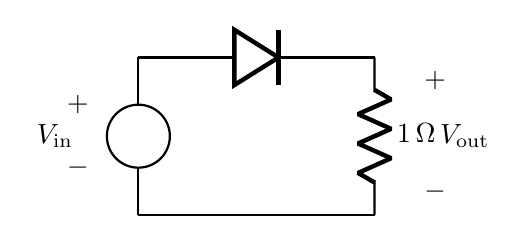
\begin{tikzpicture}[thick,scale=1.0]
            % Input Voltage Source
            \draw (0,1) circle (0.4);
            \node[left] at (-0.5, 1.4) {$+$};
            \node[left] at (-0.5, 0.6) {$-$};
            \node[left] at (-0.7, 1) {$V_{\text{in}}$};
            \draw (0,0) -- (0,0.6);
            \draw (0,1.4) -- (0,2);
            
            % Diode Connection
            \draw (0,2) -- (0.5,2);
            \draw (0.5, 2) to[D] (2.5, 2);
            \draw (2.5,2) -- (3,2);
            
            % Output Resistor (1 Ohm)
            \draw (3,2) to[R, l=$1\,\Omega$] (3,0);
            
            % Output Voltage Labels
            \node[right] at (3.5, 1.7) {$+$};
            \node[right] at (3.5, 0.3) {$-$};
            \node[right] at (3.7, 1) {$V_{\text{out}}$};
            
            % Bottom Wire Connection
            \draw (3,0) -- (0,0);
        \end{tikzpicture}

    % ===================================================
    % Figure 2: V-I Characteristic Graph

        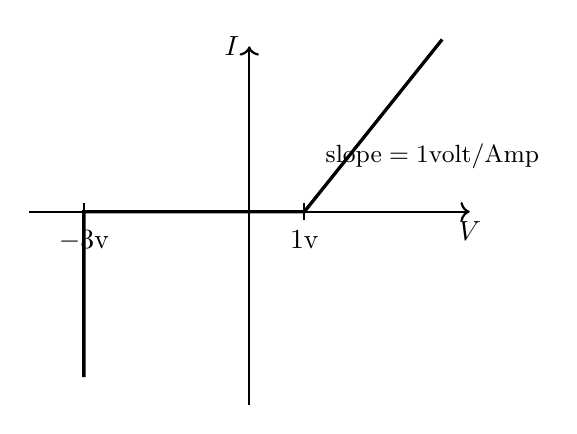
\begin{tikzpicture}[thick,scale=0.7]
            % Axes
            \draw[->] (-4, 0) -- (4, 0) node[below] {$V$};
            \draw[->] (0, -3.5) -- (0, 3) node[left] {$I$};

            % Curve
            \draw[very thick] (-3, -3) -- (-3, 0) -- (1, 0) -- (3.5, 3.125);

            % Labels and Ticks
            \draw (-3, 0.15) -- (-3, -0.15) node[below] {$-3\text{v}$};
            \draw (1, 0.15) -- (1, -0.15) node[below] {$1\text{v}$};
            \node[right] at (1.2, 1.0) {\small $\text{slope} = 1\text{volt/Amp}$};
        \end{tikzpicture}

    % ===================================================
    % Figure 3: Staircase Waveform Graph
    % ===================================================

        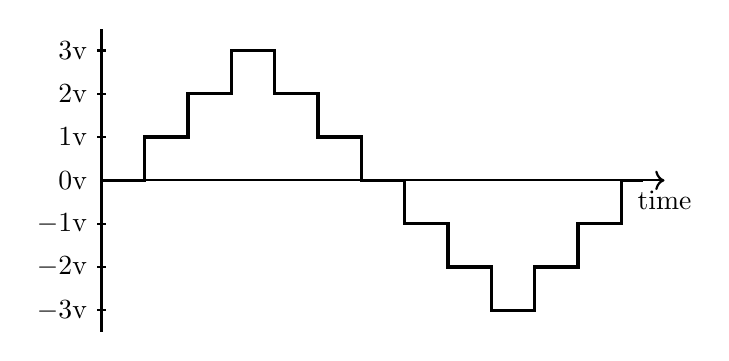
\begin{tikzpicture}[thick,scale=0.55]
            % Axes
            \draw[->] (0, 0) -- (13, 0) node[below] {time};
            \draw (0, -3.5) -- (0, 3.5);

            % Y-axis labels
            \foreach \y in {-3,-2,-1, 1,2,3} {
                \draw (-0.1, \y) -- (0.1, \y);
                \node[left] at (-0.1, \y) {$\y\text{v}$};
            }
            \node[left] at (-0.1, 0) {$0\text{v}$};

            % Staircase Curve
            \draw[very thick] (0,0) 
                -- (1,0) -- (1,1)
                -- (2,1) -- (2,2)
                -- (3,2) -- (3,3)
                -- (4,3) -- (4,2)
                -- (5,2) -- (5,1)
                -- (6,1) -- (6,0)
                -- (7,0) -- (7,-1)
                -- (8,-1) -- (8,-2)
                -- (9,-2) -- (9,-3)
                -- (10,-3) -- (10,-2)
                -- (11,-2) -- (11,-1)
                -- (12,-1) -- (12,0) -- (12.5,0);
        \end{tikzpicture}
\end{center}

\item The I-V characteristics of a diode and a sinusoidal input voltage signal $V_{in}$ are given in the figure. Draw the output voltage $V_{out}$ across the resistor.
\mk{16} 
\item What would be the output voltage $V_{out}$ across the resistor if the diode had a constant 0.7\,V voltage drop?
\mk{10} 

\end{enumerate}


\item
\begin{enumerate}\item An AC voltage source is applied to a series combination of a diode and a resistance. The dotted line in the figure is the input voltage waveform ($V_{ac}$) and the solid line is the output voltage waveform ($V_R$) across the resistance. Copy $V_R$ from the figure to your answer script exactly to scale and draw the voltage waveform across the diode over the same graph. Given that $\frac{dV_{ac}}{dt}=1\,\text{V/sec}$ when $V_{ac}$ is rising and $\frac{dV_{ac}}{dt}=-1\,\text{V/sec}$ when $V_{ac}$ is falling.

\begin{center}
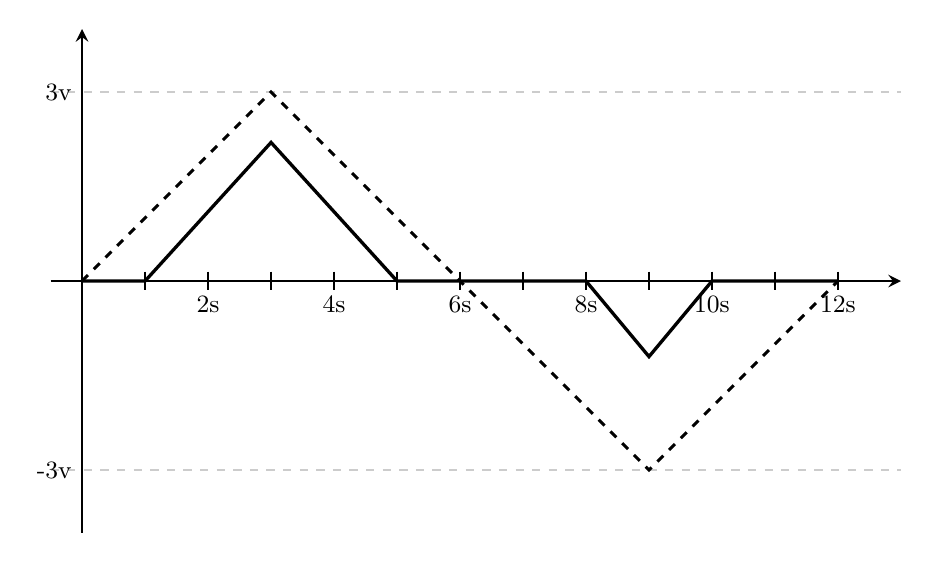
\begin{tikzpicture}[thick,scale=0.8]
    % ৩ভোল্ট এবং -৩ভোল্ট এর অনুভূমিক ডটেড গাইডলাইন
    \draw[gray!40, dashed] (-0.5, 3) -- (13, 3);
    \draw[gray!40, dashed] (-0.5, -3) -- (13, -3);
    
    % Y-axis এর লেবেল (3v এবং -3v)
    \node[left, font=\small] at (0, 3) {3v};
    \node[left, font=\small] at (0, -3) {-3v};

    % অক্ষরেখা (Axes) অংকন
    \draw[->, >=stealth, line width=1pt] (-0.5, 0) -- (13, 0); % X-axis
    \draw[->, >=stealth, line width=1pt] (0, -4) -- (0, 4);   % Y-axis

    % X-axis এর প্রতিটি ১ সেকেন্ড পর পর টিক মার্ক (Ticks)
    \foreach \x in {1,2,...,12} {
        \draw (\x, 0.15) -- (\x, -0.15);
    }
    
    % ছবিতে থাকা নির্দিষ্ট টাইম লেবেলগুলো (2s, 4s, 6s, 8s, 10s, 12s)
    \node[below, font=\small, yshift=-2pt] at (2, 0) {2s};
    \node[below, font=\small, yshift=-2pt] at (4, 0) {4s};
    \node[below, font=\small, yshift=-2pt] at (6, 0) {6s};
    \node[below, font=\small, yshift=-2pt] at (8, 0) {8s};
    \node[below, font=\small, yshift=-2pt] at (10, 0) {10s};
    \node[below, font=\small, yshift=-2pt] at (12, 0) {12s};

    % ১. ড্যাশড ওয়েভফর্ম (Dashed Triangle Wave)
    % (0,0) থেকে শুরু হয়ে 3s এ পিক (3v), 6s এ শূন্য, 9s এ নেগেটিভ পিক (-3v), 12s এ শেষ।
    \draw[dashed, line width=1.1pt] (0,0) -- (3,3) -- (6,0) -- (9,-3) -- (12,0);

    % ২. সলিড ওয়েভফর্ম (Solid Output Waveform)
    % ছবি অনুযায়ী: 1s পর্যন্ত 0, তারপর 3s এ পজিটিভ পিক, 5s এ আবার 0। 
    % এরপর 8s পর্যন্ত 0, 9s এ ছোট নেগেটিভ পিক, এবং 10s থেকে 12s পর্যন্ত আবার 0।
    \draw[very thick, black] (0,0) -- (1,0) -- (3,2.2) -- (5,0) -- (8,0) -- (9,-1.2) -- (10,0) -- (12,0);

\end{tikzpicture}
\end{center}

\mk{20} \yr{EEE 263 | L-2/T-1 | 2012--13}




\item Draw the I-V characteristics curve of the above diode exactly to scale (mention the voltage(s) at which the diode begins conduction).
\mk{16} \yr{EEE 263 | L-2/T-1 | 2012--13}

\item Draw the voltage waveform across the diode if it had been connected in parallel to the resistance.
\mk{10} \yr{EEE 263 | L-2/T-1 | 2012--13}

\end{enumerate}


\end{enumerate}

%%──────────────────────────────────────────────────────────────────────
\subtopic{cA}{Diode Thermal Characteristics}
\label{sub:s1-thermal}

\begin{enumerate}\item When a 15\,A current is applied to a particular diode, the junction voltage immediately becomes 0.7\,V. As power dissipation raises its temperature, the voltage eventually reaches 0.6\,V. (i) What is the apparent rise in junction temperature? (ii) What is the temperature rise per watt of power dissipation? (iii) What is the power dissipated in the diode in its final state?
\mk{15} \yr{EEE 263 | L-2/T-1 | 2024--25}

\item When a 15\,A current is applied to a particular diode, the junction voltage immediately becomes 0.7\,V. As power dissipation raises its temperature, the voltage eventually reaches 0.58\,V.\\
 (i) What is the apparent rise in junction temperature? \\
 (ii) What is the temperature rise per watt of power dissipation? \\
 (iii) What is the power dissipated in the diode in its final state?\\
\mk{10} \yr{EEE 263 | L-2/T-1 | 2023--24}

\end{enumerate}

%%──────────────────────────────────────────────────────────────────────
\subtopic{cA}{Bridge Rectifier}
\label{sub:s1-rectifier}

\begin{enumerate}\item Consider a bridge rectifier circuit with a filter capacitor $C$ placed across the load resistor $R=100\,\Omega$. The transformer secondary delivers a sinusoid of 12\,V (rms) at 60\,Hz. Assume $V_D=0.8\,\text{V}$.\\
 (i) Find the value of $C$ such that the ripple voltage is no larger than 1\,V peak-to-peak. \\
 (ii) What is the DC voltage at the output? \\
 (iii) Find the load current. \\
 (iv) Find the average and peak diode currents. \\
 (v) What is the peak reverse voltage across each diode?\\
\mk{15} \yr{EEE 263 | L-2/T-1 | 2023--24}

\item A full-wave bridge rectifier circuit with 1\,k$\Omega$ load operates from a 120\,V (rms), 60\,Hz household supply through a 10:1 step-down transformer. Each diode has a voltage drop of 0.7\,V at any current. (i) What is the peak value of the rectified voltage across the load? (ii) For what fraction of a cycle does each diode conduct? (iii) What are the average voltage across and average current through the load?
\mk{10} \yr{EEE 263 | L-2/T-1 | 2023--24}

\item A full-wave bridge rectifier circuit with a 1-k$\Omega$ load operates from a 120-V (rms), 60-Hz household supply through a 10-to-1 step-down transformer having a single secondary winding. Each diode can be modeled to have a 0.7-V drop in forward bias. Find: the peak value of the rectified voltage across the load; the fraction of a cycle for which each diode conducts; the average voltage and average current through the load.
\mk{16} \yr{EEE 263 | L-2/T-1 | 2022--23}

\item For the bridge rectifier circuit shown, $v_s$ is a 12\,V (rms) sinusoid, $V_D=0.7\,\text{V}$, and $R=100\,\Omega$. Find the average of the output voltage $v_o$, the peak diode current, and the PIV.
\begin{center}
    
    \begin{circuitikz}[american, thick]
        
        % AC Input Terminals
        \draw (0, 4) coordinate (in_top) to[short, o-] (1, 4);
        \draw (0, 0) coordinate (in_bot) to[short, o-] (1, 0);
        
        % AC Input Labels
        \node[left, align=center] at (-0.2, 2) {ac \\ line \\ voltage};
        \node[below right] at (0, 4) {$+$};
        \node[above right] at (0, 0) {$-$};
        
        % Transformer Primary Coil
        \draw (1, 4) to[L] (1, 0);
        
        % Transformer Core (Two parallel lines)
        \draw[thick] (1.2, 0.5) -- (1.2, 3.5);
        \draw[thick] (1.4, 0.5) -- (1.4, 3.5);
        
        % Transformer Secondary Coil
        \draw (1.6, 4) coordinate (sec_top) to[L] (1.6, 0) coordinate (sec_bot);
        
        % Transformer Secondary Labels
        \node[right] at (2.0, 3.5) {$+$};
        \node[right] at (2.0, 2.4) {$v_S$};
        \node[right] at (2.0, 0.5) {$-$};
        
        % Bridge Rectifier Nodes setup
        \coordinate (top) at (4.5, 4);
        \coordinate (bottom) at (4.5, 0);
        \coordinate (left) at (3, 2);
        \coordinate (right) at (6, 2);
        
        % Connecting Secondary to Bridge
        \draw (sec_top) -- (top);
        \draw (sec_bot) -- (bottom);
        
        % Bridge Diodes (Solid filled triangles)
        \draw (top) to[ diode, l=$D_1$] (right);       % Top-Right
        \draw (left) to[ diode, l=$D_4$] (top);        % Top-Left
        \draw (left) to[ diode, l_=$D_2$] (bottom);    % Bottom-Left
        \draw (bottom) to[ diode, l_=$D_3$] (right);   % Bottom-Right
        
        % Load Resistor R inside the bridge
        \draw (left) to[R] (right);
        \node at (4.5, 2.6) {$v_o$};
        \node at (3.8, 2.3) {$-$};
        \node at (5.2, 2.3) {$+$};
        \node at (4.5, 1.4) {$R$};
        
        % Ground Connection from the left node
        \draw (left) -- ++(-0.6, 0) coordinate (gnd);
        \node[ground] at (gnd) {};
        
        % Bridge Node dots
        \filldraw (top) circle (2pt);
        \filldraw (bottom) circle (2pt);
        \filldraw (left) circle (2pt);
        \filldraw (right) circle (2pt);
        
    \end{circuitikz}
\end{center}
\mk{15} \yr{EEE 263 | L-2/T-1 | 2021--22}

\item Draw the transfer curve of the circuit shown, assuming all diodes are ideal, $R_1=R_2=20\,\text{k}\Omega$, and $R_L=10\,\text{k}\Omega$. (i) What is the maximum peak voltage of the output signal? (ii) What is the peak-inverse voltage? (iii) What is the average current through the load?
\begin{center}
         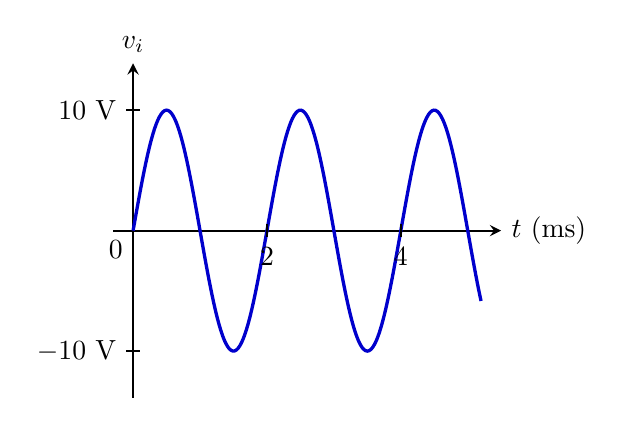
\begin{tikzpicture}[thick,scale=0.85, baseline=(current bounding box.center)]
            % Grid/Axes
            \draw[->, >=stealth, thick] (-0.3, 0) -- (5.5, 0) node[right] {$t\text{ (ms)}$};
            \draw[->, >=stealth, thick] (0, -2.5) -- (0, 2.5) node[above] {$v_i$};
            
            % Origin label
            \node[below left] at (0,0) {$0$};
            
            % Mathematical curve: Period = 2 units, Peak = 1.8 units
            % TikZ sin() expects degrees by default: \x*180 maps 1 unit to 180 degrees (half cycle)
            \draw[domain=0:5.2, samples=200, smooth, blue!80!black, very thick] 
                plot (\x, {1.8*sin(\x*180)});
            
            % X-axis ticks & labels
            \draw[thick] (2, 0.1) -- (2, -0.1) node[below] {$2$};
            \draw[thick] (4, 0.1) -- (4, -0.1) node[below] {$4$};
            
            % Y-axis ticks & labels
            \draw[thick] (0.1, 1.8) -- (-0.1, 1.8) node[left] {$10\text{ V}$};
            \draw[thick] (0.1, -1.8) -- (-0.1, -1.8) node[left] {$-10\text{ V}$};
        \end{tikzpicture}
\end{center}
\begin{center}

        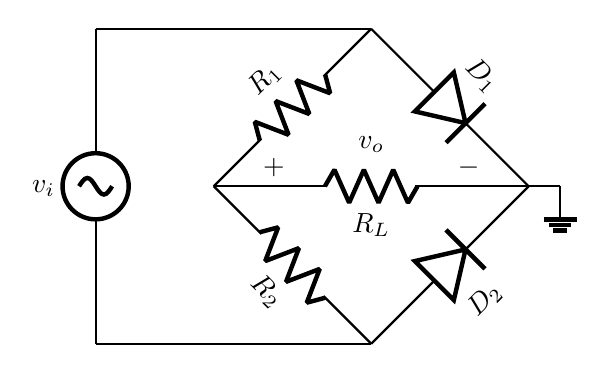
\begin{tikzpicture}[thick,scale=1.0, transform shape, baseline=(current bounding box.center)]
            % Bridge core nodes
            \coordinate (Top) at (2,2);
            \coordinate (Bottom) at (2,-2);
            \coordinate (Left) at (0,0);
            \coordinate (Right) at (4,0);
            
            % AC Voltage Source on the far left
            \draw (-1.5,-2) to[sinusoidal voltage source, l=$v_i$] (-1.5,2);
            
            % Source connections to bridge apexes
            \draw (-1.5,2) -- (Top);
            \draw (-1.5,-2) -- (Bottom);
            
            % Bridge Arms
            \draw (Top) to[R, l_=$R_1$] (Left);
            \draw (Left) to[R, l_=$R_2$] (Bottom);
            \draw (Top) to[D, l=$D_1$] (Right);
            \draw (Bottom) to[D, l_=$D_2$] (Right);
            
            % Center Load Resistor + Differential Voltage marker
            \draw (Left) to[R, l_=$R_L$, v^=$v_o$] (Right);
            
            % Ground Reference connection
            \draw (Right) -- (4.4,0) node[ground]{};
        \end{tikzpicture}

\end{center}
\mk{23} \yr{EEE 263 | L-2/T-1 | 2020--21}

\item Draw the circuit of a full-wave bridge rectifier and show the output wave shape for a sinusoidal input.
\mk{16} \yr{EEE 263 | L-2/T-1 | 2018--19}

\item For a full-wave bridge rectifier, find the value of peak current through the diode and PIV for the diode. Given: $V_s=12\,\text{V}$ (rms), $V_{DO}=0.7\,\text{V}$, $R=100\,\Omega$.
\mk{10} \yr{EEE 263 | L-2/T-1 | 2018--19}

\item Comment on the value of RC time constant for a rectifier circuit.
\mk{10} \yr{EEE 263 | L-2/T-1 | 2018--19}



\item Show that the average output voltage of a bridge rectifier circuit is $V_o = \frac{2}{\pi}V_s - 2V_{DO}$. If the input voltage is a 12\,V (rms) sinusoid and the load resistance is 100\,$\Omega$, calculate: (i) the average output voltage, (ii) the peak diode current, and (iii) the PIV of the diodes. Assume $V_{DO}=0.7\,\text{V}$.
\mk{16} \yr{EEE 263 | L-2/T-1 | 2011--12}

\end{enumerate}

%%──────────────────────────────────────────────────────────────────────
\subtopic{cA}{Zener Diode Regulator}
\label{sub:s1-zener}

\begin{enumerate}\item A 6.8\,V Zener diode exhibits its nominal voltage at a test current of 5\,mA. At this current the incremental resistance is $r_z=20\,\Omega$ and knee current $I_{ZK}=0.2\,\text{mA}$. The negative terminal is connected to $V^+=10\,\text{V}$ ($\pm1\,\text{V}$) through a $0.5\,\text{k}\Omega$ resistor; positive terminal is grounded. (i) Find $V_o$ with no load at nominal supply. (ii) Find the change in $V_o$ as supply varies by $\pm1\,\text{V}$. (iii) Find the change in $V_o$ when $R_L=2\,\text{k}\Omega$ is connected; what happens if $R_L=0.5\,\text{k}\Omega$? (iv) Find the minimum $R_L$ for which the diode still operates in breakdown.
\mk{20} \yr{EEE 263 | L-2/T-1 | 2024--25}

\item A 9.1\,V Zener diode exhibits its nominal voltage at a test current of 28\,mA. At this current the incremental resistance is specified to be 5\,$\Omega$. (i) Find $V_{z0}$ in the Zener model. (ii) Find the Zener voltage at currents of 10\,mA and 100\,mA, respectively. (iii) Comment on the advantages/disadvantages of running the Zener diode at current values other than the nominal value.
\mk{10} \yr{EEE 263 | L-2/T-1 | 2023--24}

\item For the circuit given, determine the range of $R_L$ and $I_L$ that will result in $V_{R_L}$ being maintained at 10\,V. Also determine the maximum wattage rating of the diode. The Zener diode is a 10\,V Zener with maximum current rating of 32\,mA.
\begin{center}
    \begin{circuitikz}[thick, scale=1.2, transform shape]
    
    % Input Terminals & Voltage Source Label
    \draw (0,3) node[ocirc] {} node[left, yshift=0.1cm] {$+$};
    \draw (0,0) node[ocirc] {} node[left, yshift=-0.1cm] {$-$};
    \node at (-0.6, 1.5) {$V_i = 50\text{ V}$};

    % Top Wire & Series Resistor (R below, value above)
    \draw (0,3) to[R, l_=$R$, name=R1] (4,3);
    \node[above=0.15cm] at (R1.north) {$1\text{ k}\Omega$};
    
    % Current Arrow I_R
    \draw[->, >=stealth, line width=0.8pt] (2.7, 3.5) -- (3.2, 3.5) node[midway, above] {$I_R$};

    % Zener Diode Branch (Cathode up, Anode down)
    \draw (4,0) to[zzD] (4,3);    
    % Zener Labels on the Left side
    \node[left=0.2cm, align=left] at (4, 1.5) {
        $V_Z = 10\text{ V}$ \\ 
        $I_{ZM} = 32\text{ mA}$
    };
    
    % Current Arrow I_Z on the Right side
    \draw[->, >=stealth, line width=0.8pt] (4.6, 2.2) -- (4.6, 1.4) node[midway, right] {$I_Z$};

    % Variable Load Resistor Branch (R_L)
    \draw (4,3) -- (7,3)
          to[vR, l=$R_L$] (7,0)
          -- (4,0);

    % Corner Current Arrow I_L
    \draw[->, >=stealth, line width=0.8pt] (6.5, 3.4) -- (7.4, 3.4) -- (7.4, 2.3);
    \node[right] at (7.4, 2.85) {$I_L$};

    % Bottom Return Path Wire
    \draw (0,0) -- (4,0);

\end{circuitikz}
\end{center}
\mk{18} \yr{EEE 263 | L-2/T-1 | 2022--23}

\item The zener diode in the circuit shown is specified to have $V_Z=6.8\,\text{V}$ at $I_Z=5\,\text{mA}$, $r_z=20\,\Omega$ and $I_{ZK}=0.2\,\text{mA}$. (i) Find $V_0$ at no load conditions. (ii) What is the minimum value of $R_L$ for which the diode will still operate in the breakdown region?
\begin{center}
    
    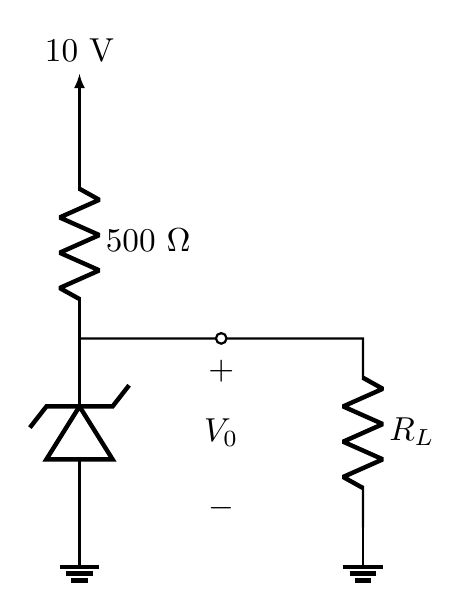
\begin{tikzpicture}[thick,scale=1.2, transform shape]
        
        % Top Voltage source arrow and label
        \draw[-latex] (0, 2) -- (0, 2.8) node[above] {$10\text{ V}$};
        
        % Top Resistor (500 Ohm)
        \draw (0, 2) to[R, l=$500\ \Omega$] (0, 0);
        
        % Zener Diode (drawn bottom-to-top so the cathode bar faces upwards)
        \draw (0, -2) node[ground]{} to[zzD] (0, 0);
        
        % Right branch to Load Resistor
        \draw (0, 0) -- (1.5, 0) node[ocirc]{} -- (3, 0) 
              to[R, l=$R_L$] (3, -2) node[ground]{};
        
        % Output Voltage Labels
        \node[below] at (1.5, -0.1) {$+$};
        \node at (1.5, -1) {$V_0$};
        \node at (1.5, -1.8) {$-$};
        
    \end{tikzpicture}
\end{center}
\mk{23} \yr{EEE 263 | L-2/T-1 | 2020--21}

\item A voltage regulator circuit is to power a car radio at $V_L=9\,\text{V}$ from an automobile battery whose voltage may vary between 11 and 13.6\,V. The current in the radio will vary between 0 (off) and 100\,mA (full volume). Determine the value of the current-limiting resistor $R_i$ and the maximum power dissipated in the Zener diode.
\begin{center}
  
    \begin{circuitikz}[thick,scale=1.2, transform shape]
        
        % ==========================================
        % Voltage Source (Left Branch)
        % ==========================================
        % Drawn from bottom to top so the positive terminal (long line) is at the top
        \draw (0,3) to[battery] (0,0);
        
        % Manual labels for the battery to match the specific formatting in the image
        \node[left, align=center] at (-0.5, 1.5) {$V_{PS} =$\\$11-13.6\text{ V}$};
        \node[left] at (-0.2, 2.6) {$+$};
        \node[left] at (-0.2, 0.4) {$-$};
        
        % ==========================================
        % Series Resistor R1 (Top Branch)
        % ==========================================
        \draw (0,3) to[R, l=$R_1$, i=$I_I$] (4,3);
        
        % ==========================================
        % Zener Diode (Middle Branch)
        % ==========================================
        % Drawn from top to bottom. "invert" flips the diode so the cathode is facing up.
        % The current I_Z is drawn flowing downwards.
        \draw (4,3) to[zzD, invert, i=$I_Z$, *-*] (4,0);
        
        % Voltage labels for the Zener Diode
        \node[right] at (4.2, 2.5) {$+$};
        \node[right] at (4.2, 1.5) {$V_Z = 9\text{ V}$};
        \node[right] at (4.2, 0.5) {$-$};
        
        % ==========================================
        % Load - Radio (Right Branch)
        % ==========================================
        % Top wire with load current arrow
        \draw (4,3) to[short, i=$I_L$] (7.5,3);
        
        % Shaded Radio box
        \node[draw, fill=gray!30, minimum width=1.5cm, minimum height=1.2cm] (radio) at (7.5, 1.5) {Radio};
        
        % Connecting lines to the Radio box
        \draw (7.5,3) -- (radio.north);
        \draw (radio.south) -- (7.5,0);
        
        % ==========================================
        % Bottom Ground/Return Wire
        % ==========================================
        \draw (7.5,0) -- (0,0);

        
    \end{circuitikz}
\end{center}
\mk{18} \yr{EEE 263 | L-2/T-1 | 2017--18}

\item For the circuit shown in Figure , plot $v_0$ versus $v_{\text{i}}$ and $i_1$ versus $v_{\text{i}}$ over the range $-10 \le v_{\text{i}} \le +10\text{ V}$. Assume the diodes to be ideal.
 \begin{center}
\begin{circuitikz}[thick,scale=1.2, transform shape]
        
        % ==========================================
        % Input Stage
        % ==========================================
        % Input terminal and 10k Resistor with current label i_i
        \draw (0, 3) node[left] {\Large $v_i$} node[ocirc] {} 
              to[R, l=$10\text{ k}\Omega$, i_=$i_i$] (3, 3);
              
        % ==========================================
        % Zener Diode Section
        % ==========================================
        % Zener drawn right-to-left so it points left (cathode on the left)
        \draw (5, 3) to[zzD] (3, 3);
        
        % Manual placement for Zener labels (+, -, and Vz)
        \node at (3.3, 3.4) {\large $+$};
        \node at (4.7, 3.4) {\large $-$};
        \node at (4.0, 3.8) {$V_z=3\text{V}$};
        
        % ==========================================
        % Top Rail and Output
        % ==========================================
        % Junction dots
        \node[circ] at (5, 3) {};
        \node[circ] at (6.5, 3) {};
        
        % Wire extending to output terminal
        \draw (5, 3) -- (7.5, 3) node[ocirc] {} node[right] {\Large $v_o$};
        
        % ==========================================
        % Vertical Branches
        % ==========================================
        % Standard Diode pointing UP (cathode on top)
        \draw (5, 0) to[D] (5, 3);
        
        % 10k Output Resistor
        \draw (6.5, 3) to[R, l=$10\text{ k}\Omega$] (6.5, 0);
        
        % ==========================================
        % Ground Connection
        % ==========================================
        % Connect bottoms and attach ground
        \draw (5, 0) -- (6.5, 0);
        \node[ground] at (5.75, 0) {};
        
    \end{circuitikz}
\end{center}
\mk{13.67} \yr{EEE 263 | L-2/T-1 | 2016--17}


\item For the circuit shown, find $V_a$ and $I_z$. Now if $R_1$ and $R_2$ are swapped, what will be the value of $V_a$ and $I_z$?

\begin{center}
  
    \begin{circuitikz}[thick,scale=1.2, transform shape]
        
        % ১. DC Voltage Source
        % battery1 ব্যবহার করলে ডিফল্টভাবে উপরের দিকে পজিটিভ (বড় দাগ) থাকে
        \draw (0,2.5) to[battery1] (0,0);
        \node at (-0.6, 2.2) {$+$};
        \node at (-0.7, 1.25) {$10\mathrm{V}$};
        \node at (-0.6, 0.3) {$-$};
        
        % ২. R1 Resistor and Top Wire
        \draw (0,2.5) to[R, l={$R_1=2\mathrm{K}\Omega$}] (3,2.5) coordinate (top_mid);
        \draw (0,0) -- (3,0) coordinate (bot_mid);
        
        % ৩. Zener Diode Branch
        % জেনার ডায়োডটি নিচ থেকে উপরে আঁকা হয়েছে যেন ক্যাথোড (দাগ দেওয়া অংশ) উপরে থাকে
        \draw (bot_mid) to[zzD] (top_mid); 
        
        % Zener Labels (Current and Voltage)
        % Iz কারেন্টের জন্য আলাদা একটি তীর (arrow) আঁকা হয়েছে
        \draw[->, >=stealth] (2.4, 1.8) -- (2.4, 0.7) node[midway, left] {$I_Z$};
        \node[right, align=left] at (3.4, 1.25) {$5\mathrm{V}$\\zener};
        
        % ৪. R2 Resistor Branch
        \draw (top_mid) -- (5,2.5) coordinate (top_right);
        \draw (bot_mid) -- (5,0) coordinate (bot_right);
        \draw (top_right) to[R, l={$R_2=3\mathrm{K}\Omega$}] (bot_right);
        
        % ৫. Output Terminals (Vo)
        \draw (top_right) to[short, -o] (6,2.5) node[above] {$+$};
        \draw (bot_right) to[short, -o] (6,0) node[below] {$-$};
        \node[right] at (6,1.25) {$V_o$};

        
    \end{circuitikz}
\end{center}

\mk{15} \yr{EEE 263 | L-2/T-1 | 2015--16}

\item Calculate the regulated load voltage $V_L$ and the current $I_Z$ flowing through the zener diode in the voltage regulator circuit shown.


\begin{center}
      \begin{circuitikz}[thick,scale=1.2, transform shape]
        
        % ===================================================
        % Zener Diode & BJT Regulator Circuit
        % ===================================================
        
        % 1. Input 30V DC Source
        \draw (0,3) to[battery1, l={$30\mathrm{V}$}] (0,0) node[ground]{};
        
        % 2. 1.5k Ohm Resistor on top wire
        \draw (0,3) to[R, l={$1.5\mathrm{k}\Omega$}] (3,3);
        
        % 3. Zener Diode branch
        % Drawn from bottom to top so the cathode (bar) is at the top
        \draw (3,1.5) to[zzD, l_={$V_Z=9.3\mathrm{V}$}] (3,3);
        
        % Iz Current Arrow (drawn manually for exact placement like the image)
        \draw[->, >=stealth] (2.2, 2.7) -- (2.2, 1.8) node[midway, left] {$I_Z$};
        
        % 4. NPN BJT (Positioned cleanly at coordinates 5, 1.5)
        \node[npn] (Q1) at (5, 1.5) {};
        \node at (6.1, 1.5) {$\beta_{DC}=100$};
        
        % 5. Connections to BJT using its built-in anchors (Base, Collector, Emitter)
        % Base connection from Zener branch junction to Q1.B
        \draw (3,1.5) node[circ]{} -- (Q1.B);
        
        % Collector connection going UP from Q1.C to the top wire
        \draw (Q1.C) -- (5,3);
        
        % Emitter connection going DOWN from Q1.E to ground
        \draw (Q1.E) -- (5,0) node[ground]{};
        
        % 6. Top wire connecting Zener, BJT Collector, and Output
        \draw (3,3) node[circ]{} -- (5,3) node[circ]{} -- (7.5,3);
        
        % 7. Output terminal and Load Resistor (RL)
        \draw (7.5,3) node[ocirc]{} to[R, l={$R_L=1\mathrm{k}\Omega$}] (7.5,0) node[ground]{};
        
        % 8. VL Voltage Label (+, arrow, -) placed left of the load resistor
        \node at (9.7, 2.7) {$+$};
        \draw[->, >=stealth] (9.7, 2.4) -- (9.7, 0.6) node[midway, right] {$V_L$};
        \node at (9.7, 0.3) {$-$};
        
    \end{circuitikz}
\end{center}
\mk{16} \yr{EEE 263 | L-2/T-1 | 2014--15}

\end{enumerate}

%%──────────────────────────────────────────────────────────────────────
\subtopic{cA}{Diode Circuit Design}
\label{sub:s1-design}

\begin{enumerate}\item Design the circuit shown to provide an output voltage $v_a = 3\,\text{V}$. Assume that the diodes available have 0.7\,V drop at 1\,mA, thermal voltage = 25\,mV, and parameter $n=1$.
\begin{center}
      \begin{circuitikz}[thick,scale=1.2, transform shape]
        
        % ১. +10V Source Terminal (কাস্টম ত্রিভুজ)
        % হুবহু হাতে আঁকা ছবির মতো একটি উপরের দিকে মুখ করা ত্রিভুজ আঁকা হয়েছে
        \draw (0, 4.6) -- (0, 4.7);
        \draw (0, 5.0) -- (-0.2, 4.7) -- (0.2, 4.7) -- cycle;
        \node[above] at (0, 5.0) {\large $+10\mathrm{V}$};
        
        % ২. Resistor R
        \draw (0, 4.6) to[R, l=$R$] (0, 2.5);
        
        % ৩. Diodes in Series (৪টি ডায়োড)
        % ডায়োডগুলো ক্রমান্বয়ে নিচে নামানো হয়েছে
        \draw (0, 2.5) to[D] (0, 1.5)
              to[D] (0, 0.5)
              to[D] (0, -0.5)
              to[D] (0, -1.5);
        
        % ৪. Ground Connection
        \draw (0, -1.5) node[ground] {};
        
        % ৫. Output Terminal (Vo)
        \fill (0, 2.5) circle (1.5pt); % জাংশন ডট
        \draw (0, 2.5) to[short, -o] (1.5, 2.5) node[below=2pt] {$+$};
        
        % ৬. Vo Label and minus (-) sign
        % Vo এবং মাইনাস চিহ্ন ডানদিকে পজিশন করা হয়েছে
        \node at (1.5, 0.5) {\Large $V_o$};
        \node at (1.5, -1.5) {\Large $-$};
        
    \end{circuitikz}
\end{center}
\mk{15} \yr{EEE 263 | L-2/T-1 | 2015--16}

\end{enumerate}

%%──────────────────────────────────────────────────────────────────────
\subtopic{cA}{Full Wave Rectifier}
\label{sub:s1-fwr}  


\begin{enumerate}
    
    \item Draw the circuit of a full-wave rectifier with center-tapped secondary winding and draw the input and output voltage waveshapes. Comment on the values of RC time constant for a rectifier circuit.
\mk{20} \yr{EEE 263 | L-2/T-1 | Jan--2021}  
    
    \item Draw the circuit diagram of a full wave rectifier with a filter capacitor. Assume the input is a sinusoidal signal with 10\,kHz frequency and 7.07\,V rms voltage, the load is 1\,k$\Omega$ and capacitor used is 1\,$\mu$F. Diode has a forward voltage drop of 0.7\,V. Find:
\begin{enumerate}\item Ripple voltage.
  \item PIV and duty cycle.
  \item Peak output voltage.
\end{enumerate}
\mk{16} \yr{EEE 263 | L-2/T-1 | 2015--16}


\end{enumerate}

%%──────────────────────────────────────────────────────────────────────
\subtopic{cA}{Battery Charger Circuit}
\label{sub:s1-battery}

\begin{enumerate}
    
\item The circuit shown is for charging a 5\,V battery with $V_s = 10\sin(100\pi t)$. Find:
\begin{enumerate}
  \item Duty cycle (fraction of each cycle during which the diode conducts).
  \item Draw the diode current waveform indicating peak value.
  \item Maximum reverse bias voltage that appears across the diode.
\end{enumerate}
\begin{center}
      \begin{circuitikz}[thick,scale=1.2, transform shape]
        
        % 1. AC Source (Left Branch)
        \draw (0,0) to[sV] (0,2.5);
        \node[left] at (-0.4, 1.25) {$v_s$};
        \node at (-0.3, 2.1) {$+$};
        \node at (-0.3, 0.4) {$-$};
        
        % 2. Top Branch (Resistor & Diode)
        % i=$i_D$ দিয়ে ডায়োডের সাথে কারেন্টের দিক দেখানো হয়েছে
        \draw (0,2.5) to[R, l=$100\Omega$] (2.5, 2.5) 
              to[D, i=$i_D$] (5, 2.5);
        
        % 3. DC Source / Battery (Right Branch)
        \draw (5, 2.5) to[battery1] (5, 0);
        \node[right] at (5.3, 1.25) {$5\mathrm{V}$};
        \node at (4.6, 2.1) {$+$};
        \node at (4.6, 0.4) {$-$};
        
        % 4. Bottom Branch (Wire)
        \draw (0,0) -- (5,0);
        
    \end{circuitikz}
\end{center}
\mk{15} \yr{EEE 263 | L-2/T-1 | 2015--16}

\item A circuit for charging a 10\,V battery is shown in the figure. If $V_s$ is a sinusoid with 20\,V peak amplitude, find the fraction of each cycle during which the diode conducts. Assume the diode is ideal. Also find the peak value of the diode current and the maximum reverse bias voltage that appears across the diode.

\begin{center}
\begin{circuitikz}[thick,american, thick, scale=1.2, transform shape]
  
  % Left branch (Voltage Source)
  \draw (0,3) to[V, l=$v_s$] (0,0);
  
  % Top branch (Resistor and Diode)
  \draw (0,3) to[R, l_=$100\,\Omega$] (3,3)
        to[D] (6,3);
  
  % Right branch (Battery)
  \draw (6,3) to[battery1] (6,0);
  
  % Manual labels for the 10V battery
  \node at (6.6, 2.5) {$+$};
  \node at (6.6, 1.5) {$10\text{V}$};
  \node at (6.6, 0.5) {$-$};
  
  % Bottom return wire
  \draw (0,0) -- (6,0);
  
\end{circuitikz}
\end{center}

\mk{15} \yr{EEE 263 | L-2/T-1 | 2011--12}

\end{enumerate}

%%──────────────────────────────────────────────────────────────────────
\subtopic{cA}{Diode Wave Shaping}
\label{sub:s1-waveshape}

\begin{enumerate}\item For a sinusoidal input, draw the output waveshape for the circuit shown.
\begin{center}
    \begin{circuitikz}[thick,american, scale=1.2]
    % 1. Top wire with Input terminal, Resistor R, and Output terminal
    \draw (0,2.5) node[below=2pt] {$+$} 
          to[R, l_=$R$, o-*] (3,2.5) 
          to[short, -o] (5,2.5) node[below=2pt] {$+$};
          
    % 2. Bottom reference wire with Input and Output terminals
    \draw (0,0) node[above=2pt] {$-$} 
          to[short, o-*] (3,0) 
          to[short, -o] (5,0) node[above=2pt] {$-$};
          
    % 3. Input and Output Voltage Labels
    \node[font=\large] at (0.5, 1.25) {$V_i$};
    \node[font=\large] at (4.5, 1.25) {$V_o$};
    
    % 4. Shunt Branch: Battery (V) and Diode pointing upwards
    % Drawing from bottom to top automatically sets up the correct polarities
    \draw (3,1.25) to[battery2, l_=$V$] (3,0);
        \draw (3,1.25)  to[D] (3,2.5);
          
    % 5. Figure Caption

\end{circuitikz}
\end{center}
\mk{10} \yr{EEE 263 | L-2/T-1 | 2018--19}


\item Assuming that the diodes are ideal, find the output voltage $V_o$ for the circuit given. Draw the wave shape clearly.

\begin{center}
  
    \begin{circuitikz}[thick,scale=1.1]
        
        % ===================================================
        % 1. Left Side: Input Voltage Waveform (Graph)
        % ===================================================
        \coordinate (Origin) at (0,0);
        
        % Y-axis & X-axis
        \draw[->, >=stealth] (Origin |- 0,-2) -- (Origin |- 0,2) node[above] {$v_{in}(\mathrm{Volt})$};
        \draw[->, >=stealth] (Origin) -- (5,0) node[right] {$t(\mathrm{ms})$};
        
        % Y-axis Labels (+10 and -10)
        \draw (-0.1, 1.5) -- (0.1, 1.5) node[left=0.2cm] {$+10$};
        \draw (-0.1, -1.5) -- (0.1, -1.5) node[left=0.2cm] {$-10$};
        
        % Dashed guidelines for peaks
        \draw[dashed] (0, 1.5) -- (1.25, 1.5);
        \draw[dashed] (0, -1.5) -- (3.75, -1.5);
        
        % Triangular Waveform
        \draw[thick] (0,0) -- (1.25, 1.5) 
                     -- (2.5, 0) node[below, yshift=-0.1cm] {$5$} 
                     -- (3.75, -1.5) 
                     -- (5, 0) node[below] {$10$};
                     
        % Label Vin near the axis end as in the image
        
        
    \end{circuitikz}
\end{center}


\begin{center}
    
    \begin{circuitikz}
        % ===================================================
        % 2. Right Side: Circuit Diagram
        % ===================================================
        % Shift the starting point of the circuit to the right to avoid overlap
        \coordinate (C_offset) at (8.5, 0); 
        
        % AC Voltage Source
        \draw (C_offset |- 0,-1.5) to[sV, l={$v_{in}$}] (C_offset |- 0,1.5) coordinate (TopLeft);
        
        % Resistor R at the top
        \draw (TopLeft) to[R, l={$R=10\Omega$}] ++(2.5, 0) coordinate (Node1);
        
        % Branch 1: D1 (pointing down) and 6V Battery (positive/long line UP)
        % l_ moves the labels to the left side of this branch
        \draw (Node1) to[D, l_={$D1$}] ++(0, -1.5) 
                      to[battery1, l_={$6\mathrm{V}$}] ++(0, -1.5) coordinate (Bot1);
        
        % Branch 2: D2 (pointing UP) and 4V Battery (negative/short line UP)
        % Increased distance between branches (from 1.5 to 2.0)
        \draw (Node1) -- ++(2.0, 0) coordinate (Node2);
        \coordinate (Bot2) at (Node2 |- Bot1);
        
        % Drawn from bottom to top. l_ moves labels to the right side of this branch
        \draw (Bot2) to[battery1, l_={$4\mathrm{V}$}] ++(0, 1.5) 
                     to[D, l_={$D2$}] (Node2); 
        
        % Branch 3: Series Capacitor C
        \draw (Node2) to[C, l={$C$}] ++(2, 0) coordinate (Node3);
        
        % Branch 4: D3 (pointing UP)
        \coordinate (Bot3) at (Node3 |- Bot1);
        \draw (Bot3) to[D, l_={$D3$}] (Node3);
        
        % Output Terminals (Vo) 
        % Extended the wire to 1.5 to move Vo further right
        \draw (Node3) to[short, -o] ++(1.5, 0) coordinate (OutTop);
        \draw (Bot3) to[short, -o] ++(1.5, 0) coordinate (OutBot);
        
        % Output Voltage Label (+ and - with Vo)
        \draw (OutTop) to[open, v^={$V_o$}] (OutBot);
        
        % Connect all bottom ground/return wires
        \draw (C_offset |- 0,-1.5) -- (OutBot);
        
    \end{circuitikz}
\end{center}

\mk{20} \yr{EEE 263 | L-2/T-1 | 2014--15}

\end{enumerate}


\subtopic{cA}{Special Purpose Diodes/Thyristors}
\label{sub:s1-spd}

\begin{enumerate}\item  Draw the circuit diagram of controlled full wave rectifier using SCR. Draw the waveforms of sinusoidal input, gate pulses and rectified output.
\mk{11.67} \yr{EEE 263 | L-2/T-1 | 2014--15}

\item Explain SCR and TRIAC operation with suitable examples.
\mk{15} \yr{EEE 263 | L-2/T-1 | 2013--14}

\item Sketch the output wave form of the following circuit given in Fig. for Q. 1(c)(i) assuming output wave is obtained across the resistance. The input waveform and gate pulse sequence is given in Fig. for Q. 1(c)(ii). 


\subsection*{1. Circuit Diagram [Fig. 1(c)(i)]}
\begin{center}
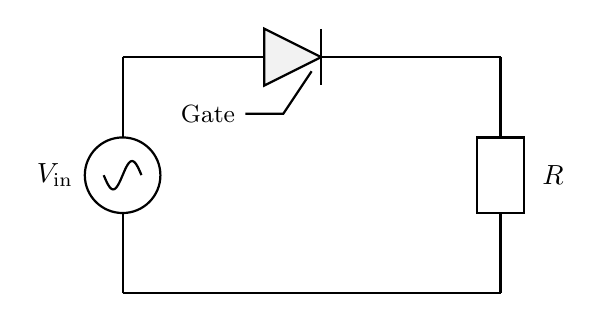
\begin{tikzpicture}[thick,scale=1.2, thick]
    % Bottom connection wire
    \draw (0,0) -- (4,0);
    
    % Left side: AC Input Voltage Source (Manual Draw)
    \draw (0,0) -- (0,0.85);
    \draw (0,1.25) circle (0.4cm);
    % Sine wave inside the circle
    \draw[smooth, samples=50, domain=-0.2:0.2] plot (\x, {1.25 + 0.15*sin(\x*360/0.4)});
    \node[left=0.5cm] at (0,1.25) {$V_{\text{in}}$};
    \draw (0,1.65) -- (0,2.5);
    
    % Top wire to SCR
    \draw (0,2.5) -- (1.5,2.5);
    
    % --- Pure TikZ SCR Symbol (Centered at x=1.85) ---
    % Diode Triangle
    \draw[fill=black!5] (1.5,2.8) -- (1.5,2.2) -- (2.1,2.5) -- cycle;
    % Cathode Bar
    \draw (2.1,2.8) -- (2.1,2.2);
    % Gate Terminal (Coming out diagonally from cathode side)
    \draw (2.0,2.35) -- (1.7,1.9) -- (1.3,1.9) node[left, font=\small] {Gate};
    
    % Wire from SCR to Resistor
    \draw (2.1,2.5) -- (4,2.5);
    
    % Right side: Load Resistor (Standard Rectangle for 100% compatibility)
    \draw (4,2.5) -- (4,1.65);
    \draw (3.75,1.65) rectangle (4.25,0.85);
    \node[right=0.4cm] at (4,1.25) {$R$};
    \draw (4,0.85) -- (4,0);
\end{tikzpicture}
\end{center}


\subsection*{2. Input Voltage Waveform [Fig. 1(c)(ii)]}
\begin{center}
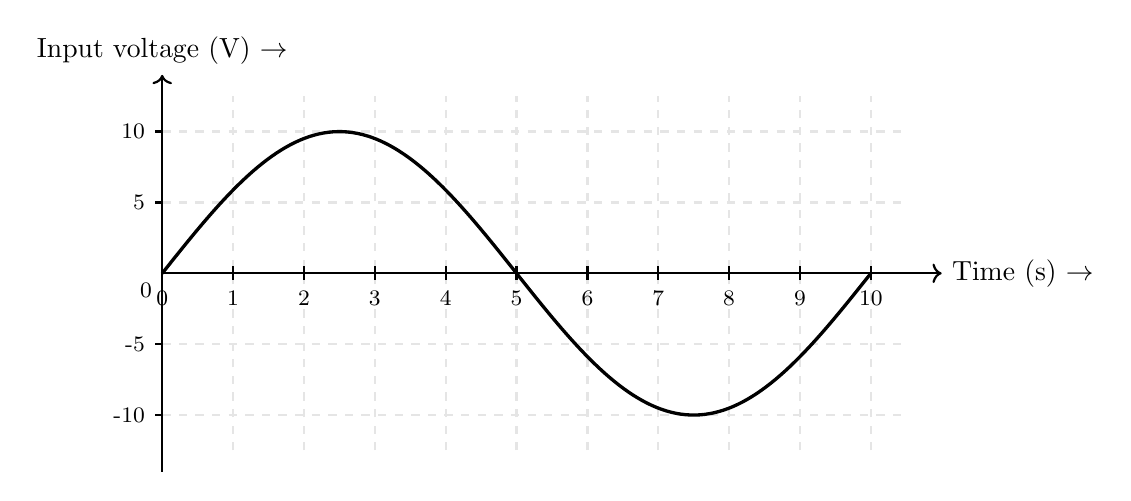
\begin{tikzpicture}[thick,scale=0.9]
    % Grid lines (dashed, light gray)
    \draw[step=1cm, gray!20, dashed] (0,-2.5) grid (10.5,2.5);

    % Axes
    \draw[->, thick] (0,0) -- (11,0) node[right] {Time (s) $\rightarrow$};
    \draw[->, thick] (0,-2.8) -- (0,2.8) node[above] {Input voltage (V) $\rightarrow$};
    
    % X-axis Ticks and Labels (0 to 10)
    \foreach \x in {0,1,...,10} {
        \draw (\x,0.1) -- (\x,-0.1);
        \node[below, font=\footnotesize] at (\x,-0.1) {\x};
    }
    
    % Y-axis Ticks and Labels (-10, -5, 5, 10) -> Scaled: 1 unit = 5V
    \draw (0,1) -- (-0.1,1) node[left, font=\footnotesize] {5};
    \draw (0,2) -- (-0.1,2) node[left, font=\footnotesize] {10};
    \draw (0,-1) -- (-0.1,-1) node[left, font=\footnotesize] {-5};
    \draw (0,-2) -- (-0.1,-2) node[left, font=\footnotesize] {-10};
    \node[below left, font=\footnotesize] at (0,0) {0};

    % Sine Wave Plotting: Max amplitude 10V (mapped to 2 units on Y)
    % One full cycle (2*pi) spans from x=0 to x=10
    \draw[very thick, black] plot[domain=0:10, samples=150] (\x, {2*sin(\x*360/10)});
\end{tikzpicture}
\end{center}

\vspace{1cm}


\subsection*{3. Gate Pulse Sequence [Fig. 1(c)(ii)]}
\begin{center}
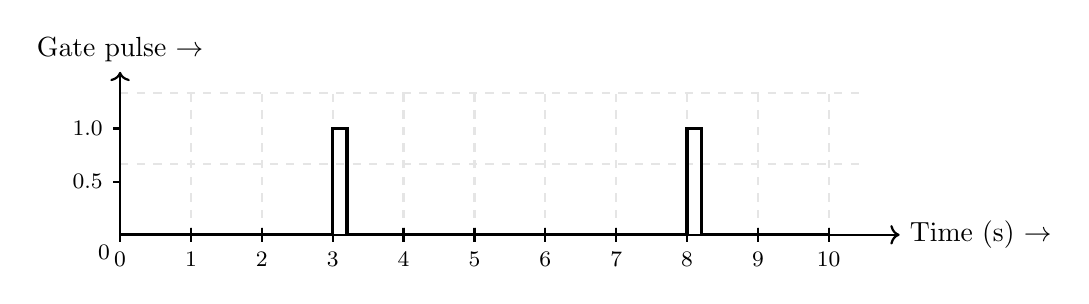
\begin{tikzpicture}[thick,scale=0.9]
    % Grid lines
    \draw[step=1cm, gray!20, dashed] (0,0) grid (10.5,2);

    % Axes
    \draw[->, thick] (0,0) -- (11,0) node[right] {Time (s) $\rightarrow$};
    \draw[->, thick] (0,0) -- (0,2.3) node[above] {Gate pulse $\rightarrow$};
    
    % X-axis Ticks and Labels
    \foreach \x in {0,1,...,10} {
        \draw (\x,0.1) -- (\x,-0.1);
        \node[below, font=\footnotesize] at (\x,-0.1) {\x};
    }
    
    % Y-axis Ticks and Labels
    \draw (0,0.75) -- (-0.1,0.75) node[left, font=\footnotesize] {0.5};
    \draw (0,1.5) -- (-0.1,1.5) node[left, font=\footnotesize] {1.0};
    \node[below left, font=\footnotesize] at (0,0) {0};

    % Drawing the pulse sequence (Triggers at t=3 and t=8)
    % Height is 1.5 units (representing 1.0V or logic high)
    \draw[very thick, black] (0,0) -- (3,0) 
                          -- (3,1.5) -- (3.2,1.5) -- (3.2,0) 
                          -- (8,0) 
                          -- (8,1.5) -- (8.2,1.5) -- (8.2,0) 
                          -- (10,0);
\end{tikzpicture}
\end{center}

\mk{20} \yr{EEE 263 | L-2/T-1 | 2011--12}


\item Draw the I-V characteristics of an SCR and a TRIAC.
\mk{10} \yr{EEE 263 | L-2/T-1 | 2011--12}

\item Explain the operating principle of a Silicon controlled Rectifier with the help of 'Two transistor model'.
\mk{20} \yr{EEE 263 | L-2/T-1 | 2011--12}



\end{enumerate}


%% ══════════════════════════════════════════════════════════════════════
%%  SECTION 2: BJT CHARACTERISTICS
%% ══════════════════════════════════════════════════════════════════════
\secdivider{S2 --- BJT Characteristics}{Energy band profiles, DC analysis, biasing stability, circuit design}{cA}

\markboth{S2: BJT Characteristics}{S2: BJT Characteristics}
\label{sec:S2}
\section*{S2 \quad BJT Characteristics}
\addcontentsline{toc}{section}{S2: BJT Characteristics}

%%──────────────────────────────────────────────────────────────────────
\subtopic{cA}{Energy Band Profile}
\label{sub:s2-energy}

\begin{enumerate}\item Draw the energy band profile of a pnp transistor under zero bias and forward-active mode bias conditions.
\mk{16/23} \yr{EEE 263 | L-2/T-1 | 2020--21, 2018--19}

\end{enumerate}

%%──────────────────────────────────────────────────────────────────────
\subtopic{cA}{Device Structure and Operating Principle}
\label{sub:s2-structure}

\begin{enumerate}\item Why is the third terminal (Base or Gate) used in a transistor?
\mk{10} \yr{EEE 263 | L-2/T-1 | Jan--2021}

\end{enumerate}

%%──────────────────────────────────────────────────────────────────────
\subtopic{cA}{Early Effect}
\label{sub:s2-early}

\begin{enumerate}\item What is the Early-effect in a BJT? Draw the $I$--$V$ curve of a practical BJT showing the Early effect.
\mk{10} \yr{EEE 263 | L-2/T-1 | 2023--24}

\item What is the early effect for BJT? What are the consequences of early effect on BJT behavior?
\mk{16} \yr{EEE 263 | L-2/T-1 | Jan--2021}

\item Why biasing is needed for an amplifier using BJT? Draw the output characteristics of a BJT connected in CE configuration. Define Early effect.
\mk{10.667} \yr{EEE 263 | L-2/T-1 | 2011--12}

\end{enumerate}

%%──────────────────────────────────────────────────────────────────────
\subtopic{cA}{DC Analysis}
\label{sub:s2-dc}

\begin{enumerate}
    
\item For the circuit shown, find the voltages at all nodes and the currents through all branches. Assume $\beta=100$.
\begin{center}
    
    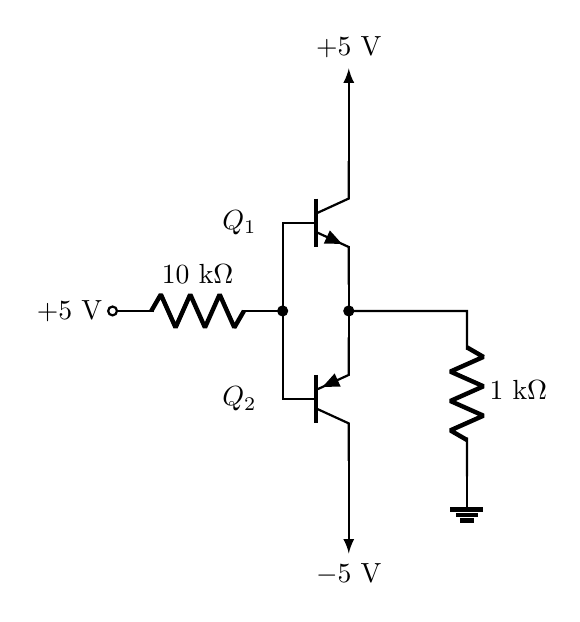
\begin{tikzpicture}[thick,x=1.5cm,y=1.4cm, transform shape]
        
        % Upper Transistor Q1 (NPN)
        \node[npn] (Q1) at (0, 0.8) {};
        \node[left=0.2cm] at (Q1.B) {$Q_1$};
        
        % Lower Transistor Q2 (PNP)
        \node[pnp] (Q2) at (0, -0.8) {};
        \node[left=0.2cm] at (Q2.B) {$Q_2$};
        
        % Connect Bases together
        \draw (Q1.B) -- (Q2.B);
        
        % Input Branch (connected to the midpoint of the bases)
        \draw (Q1.B |- 0,0) to[R, l_=$10\text{ k}\Omega$, *-o] (-2, 0) 
              node[left] {$+5\text{ V}$};
        
        % Connect Emitters together
        \draw (Q1.E) -- (Q2.E);
        
        % Output Branch (connected to the midpoint of the emitters)
        \draw (Q1.E |- 0,0) to[short, *-] (1, 0) 
              to[R, l=$1\text{ k}\Omega$] (1, -1.5) node[ground]{};
              
        % Top Power Rail (+5V)
        \draw[-latex] (Q1.C) -- (Q1.C |- 0, 2.2) node[above] {$+5\text{ V}$};
        
        % Bottom Power Rail (-5V)
        \draw[-latex] (Q2.C) -- (Q2.C |- 0, -2.2) node[below] {$-5\text{ V}$};
        
    \end{tikzpicture}
\end{center}
\mk{20} \yr{EEE 263 | L-2/T-1 | 2020--21}

\item Calculate the collector current, emitter current and base current for the circuit shown in Figure . Also verify the operating mode of the transistor. Assume $\beta = 100$. (16)

  \begin{center}
            \begin{circuitikz}[thick, american, scale=1.2]
                % NPN Transistor
                \node[npn] (Q) at (0,0) {};
                
                % Emitter to ground
                \draw (Q.E) to[R, l=$1\,\text{k}\Omega$] (0,-2) node[ground]{};
                
                % Collector up to junction
                \draw (Q.C) to[short] (0,1.5);
                
                % Resistor to VCC
                \draw (0,1.5) to[R, l=$5\,\text{k}\Omega$] (0,3);
                \draw[-latex] (0,3) -- (0,3.5) node[above] {$10\,\text{V}$};
                
                % Feedback resistor from collector junction to base
                \draw (0,1.5) to[short, *-] (-3,1.5) 
                      to[R, l=$250\,\text{k}\Omega$] (-3,0) 
                      to[short] (Q.B);
   
            \end{circuitikz}
        \end{center}
\mk{16} \yr{EEE 263 | L-2/T-1 | 2017--18}


\item Find $I_C$ and $V_{CE}$ for the circuit shown. Assume $\beta=100$.
\begin{center}
      \begin{circuitikz}[thick,scale=1.2, transform shape]
        
        % ==========================================
        % Transistor Component
        % ==========================================
        \node[npn] (Q) at (4, 0) {};
        
        % ==========================================
        % Base Circuit (Voltage Divider & Input)
        % ==========================================
        % Base junction node
        \node[circ] at (2, 0) {};
        \draw (2, 0) -- (Q.B);
        
        % Left input to base (+5V)
        \draw (0, 0) node[ocirc] {} node[left] {$+5\text{V}$} 
              to[R, l=$60\text{ k}\Omega$] (2, 0);
        
        % Top resistor at base (to +5V)
        % Drawn upwards, l_ places label on the right side
        \draw (2, 0) to[R, l_=$30\text{ k}\Omega$] (2, 2.2);
        \draw[-latex] (2, 2.2) -- (2, 2.8) node[above] {$+5\text{V}$};
              
        % Bottom resistor at base (to Ground)
        % Drawn downwards, l places label on the right side
        \draw (2, 0) to[R, l=$20\text{ k}\Omega$] (2, -2.2) node[ground] {};
              
        % ==========================================
        % Collector Circuit
        % ==========================================
        % Collector resistor (to +10V)
        \draw (Q.C) to[R, l_=$500\,\Omega$] (4, 2.2);
        \draw[-latex] (4, 2.2) -- (4, 2.8) node[above] {$+10\text{V}$};
              
        % ==========================================
        % Emitter Circuit
        % ==========================================
        % Emitter resistor (to -5V)
        \draw (Q.E) to[R, l=$200\,\Omega$] (4, -2.2);
        \draw[-latex] (4, -2.2) -- (4, -2.8) node[below] {$-5\text{V}$};
              
    \end{circuitikz}
\end{center}
\mk{16} \yr{EEE 263 | L-2/T-1 | 2016--17}

\item For the circuit shown, determine the voltages of all nodes and current through all branches. Assume $\beta=100$.
\begin{center}
      \begin{circuitikz}[thick,scale=1.2, transform shape]
        
        % ১. NPN Transistor
        \draw (2, 0) node[npn] (Q) {};
        
        % ২. Base Connection & Junction Dot
        \draw (0, 0) -- (Q.B);
        \fill (0, 0) circle (1.5pt);
        
        % ৩. Voltage Divider Bias Resistors (Base)
        % 100K Resistor (উপরের দিকে)
        \draw (0, 0) to[R, l=$100\mathrm{K}\Omega$] (0, 2.5);
        % 50K Resistor (নিচের দিকে)
        \draw (0, -2.5) to[R, l=$50\mathrm{K}\Omega$] (0, 0);
        \draw (0, -2.5) node[ground] {};
        
% ৪. Collector Branch
        \draw (Q.C) to[R, l_={$R_C = 5\mathrm{K}\Omega$}] (2, 2.5);
        
        % ৫. Emitter Branch
        \draw (2, -2.5) to[R, l_={$R_E = 3\mathrm{K}\Omega$}] (Q.E);
        \draw (2, -2.5) node[ground] {};
        
        % ৬. +15V Supply Arrows (কাস্টম ত্রিভুজ)
        % বাম দিকের অ্যারো (Base Branch)
        \draw (0, 2.5) -- (0, 2.7);
        \draw (0, 3.0) -- (-0.15, 2.7) -- (0.15, 2.7) -- cycle;
        
        % ডান দিকের অ্যারো (Collector Branch)
        \draw (2, 2.5) -- (2, 2.7);
        \draw (2, 3.0) -- (1.85, 2.7) -- (2.15, 2.7) -- cycle;
        
        % +15V লেবেল (দুটি অ্যারোর মাঝখানে উপরে)
        \node at (1, 3.3) {\Large $+15\mathrm{V}$};
        
    \end{circuitikz}
\end{center}
\mk{20} \yr{EEE 263 | L-2/T-1 | 2015--16}

\item 
\begin{enumerate}

\item Express the collector current $I_c$ as a function of $V_{CB}$ that involves the 2\,k$\Omega$ resistance (it will be a straight line equation).
\mk{16} \yr{EEE 263 | L-2/T-1 | 2012--13}

\item Find out the mathematical equation describing the $I_c$--$V_{CB}$ characteristic graph of the BJT (it will be a piecewise linear graph).
\mk{10} \yr{EEE 263 | L-2/T-1 | 2012--13}

\item Draw the two $I_c$--$V_{CB}$ graphs over the same plot exactly to scale and determine their intersection point. This intersection point gives the value of $I_c$ and $V_{CB}$ at the bias point.
\mk{10} \yr{EEE 263 | L-2/T-1 | 2012--13}

\item From the value of $V_{CB}$, can you determine the value of $V_{CE}$ at the bias point?
\mk{10} \yr{EEE 263 | L-2/T-1 | 2012--13}

\begin{center}

    \begin{circuitikz}[american, thick]

    % NPN Transistor স্থাপন করা হলো
    \draw (2,2) node[npn] (Q) {};

    % Emitter-কে গ্রাউন্ডের সাথে যুক্ত করা হলো
    \draw (Q.E) -- (2,1) node[ground] {};

    % Base-এর সাথে 1V সোর্স এবং গ্রাউন্ড যুক্ত করা হলো
    \draw (Q.B) -- (0.5,2) 
          to[battery2, l_=$1\text{V}$] (0.5,0.8) node[ground] {};

    % Collector-এর সাথে 2K\Omega রেজিস্টর এবং 5V সাপ্লাই যুক্ত করা হলো
    \draw (Q.C) to[R, l_=$2\text{K}\Omega$] (2,4.5);
    \draw[->] (2,4.5) -- (2,5.2) node[above] {$5\text{v}$};

    % V_CB নির্দেশক বাঁকা তীর চিহ্ন (Double-headed arrow)
    \draw[<->, >=stealth] (0.8,2.1) to[bend left=45] node[midway, fill=white, inner sep=1pt] {$V_{CB}$} (2,2.7);

    % path-1 নির্দেশক ধূসর রঙের বাঁকা তীর চিহ্ন
    \draw[gray, ->, >=stealth, thin] (-0.3,0.5) .. controls (-0.3,3) and (0.8,4) .. (1.8,5)
        node[pos=0.5, left, black] {path-1};

\end{circuitikz}

        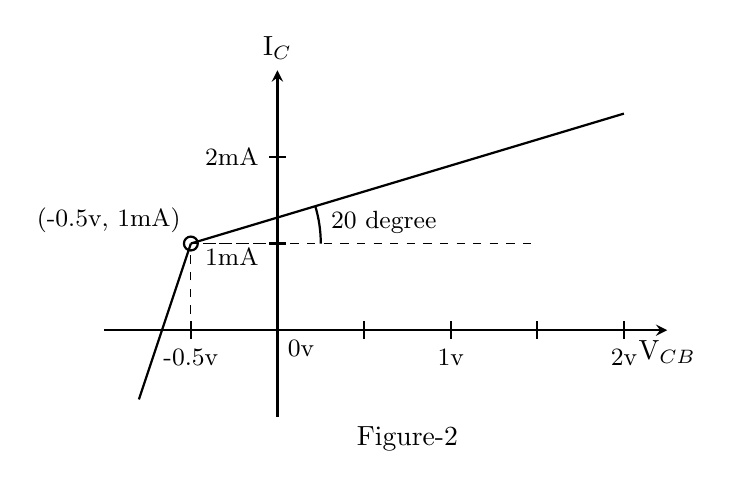
\begin{tikzpicture}[thick,scale=1.1]
            % Axes
            \draw[->, >=stealth] (-2, 0) -- (4.5, 0) node[below] {V$_{CB}$};
            \draw[->, >=stealth] (0, -1) -- (0, 3) node[above] {I$_C$};

            % Origin
            \node[below right, font=\small] at (0,0) {0v};

            % X-axis Ticks
            \draw (-1, 0.1) -- (-1, -0.1) node[below, font=\small] {-0.5v};
            \draw (1, 0.1) -- (1, -0.1); % intermediate blank tick
            \draw (2, 0.1) -- (2, -0.1) node[below, font=\small] {1v};
            \draw (3, 0.1) -- (3, -0.1); % intermediate blank tick
            \draw (4, 0.1) -- (4, -0.1) node[below, font=\small] {2v};

            % Y-axis Ticks
            \draw (0.1, 1) -- (-0.1, 1) node[below left, font=\small, yshift=2pt] {1mA}; 
            \draw (0.1, 2) -- (-0.1, 2) node[left, font=\small] {2mA};

            % Point (-0.5v, 1mA) -> mapped to coordinate (-1, 1)
            \draw[dashed, thin] (-1, 0) -- (-1, 1);
            \draw[dashed, thin] (0, 1) -- (-1, 1);
            \draw (-1, 1) circle (0.08);
            \node[above left, font=\small] at (-1, 1) {(-0.5v, 1mA)};

            % The Piecewise Linear Curve
            \draw (-1.6, -0.8) -- (-1, 1); % Steep portion
            \draw (-1, 1) -- (4, 2.5);     % Shallow portion

            % Horizontal Reference Line and Angle Arc
            \draw[dashed, thin] (-1, 1) -- (3, 1);
            \draw (0.5, 1) arc (0:16.7:1.5); % 20-degree representation arc
            \node[right, font=\small] at (0.5, 1.25) {20 degree};

            % Caption
            \node[below] at (1.5, -1) {Figure-2};
        \end{tikzpicture}
\end{center}
\end{enumerate}

\item For the circuit shown, determine $R_1$ and $R_C$ if $I_B=0.02\,\text{mA}$ and $V_{CE}=10V$.

\begin{center}
\begin{circuitikz}[thick,american, thick, scale=1.2, transform shape]
  
  % NPN Transistor
  \draw (3,3) node[npn] (Q) {};
  
  % Beta label
  \node at (4.6, 2.7) {$\beta = 150$};
  
  % Base connection
  \draw (Q.B) -- (0,3);
  
  % Left side (Base bias resistors)
  \draw (0,6) to[R, l_=$R_1$] (0,3)
        to[R, l_=$18\text{ k}\Omega$] (0,0);
        
  % Right side (Collector and Emitter resistors)
  \draw (Q.C) to[R, l_=$R_C$] (3,6);
  \draw (Q.E) to[R, l=$1.2\text{ k}\Omega$] (3,0);
  
  % Top Rail and 18V source
  \draw (0,6) -- (3,6);
  \draw[-stealth] (1.5,6) -- (1.5,6.6) node[above] {$18\text{V}$};
  
  % Bottom Rail and Ground
  \draw (0,0) -- (3,0);
  \draw (1.5,0) node[ground]{};
  
\end{circuitikz}
\end{center}

\mk{16} \yr{EEE 263 | L-2/T-1 | 2011--12}

\item Determine all node voltages and branch currents for the circuit shown. Assume $\beta=100$ and $V_{BE}=0.7\,\text{V}$.

\begin{center}
\begin{circuitikz}[thick,american, thick, scale=1.2, transform shape]
  
  % NPN Transistor
  \draw (3,3) node[npn] (Q) {};
  
  % Base connection
  \draw (Q.B) -- (0,3);
  
  % Left side (Base bias resistors)
  \draw (0,6) to[R, l_=$100\text{ k}\Omega$] (0,3)
        to[R, l_=$50\text{ k}\Omega$] (0,0);
        
  % Right side (Collector and Emitter resistors)
  \draw (Q.C) to[R, l_=$5\text{ k}\Omega$] (3,6);
  \draw (Q.E) to[R, l=$3\text{ k}\Omega$] (3,0);
  
  % Top Rail and +15V source
  \draw (0,6) -- (3,6);
  \draw[-stealth] (1.5,6) -- (1.5,6.6) node[above] {$+15\text{V}$};
  
  % Bottom Rail and Ground
  \draw (0,0) -- (3,0);
  \draw (1.5,0) node[ground]{};
  
\end{circuitikz}
\end{center}

\mk{18} \yr{EEE 263 | L-2/T-1 | 2011--12}

\end{enumerate}

%%──────────────────────────────────────────────────────────────────────
\subtopic{cA}{BJT Saturation Parameters}
\label{sub:s2-saturation}

\begin{enumerate}\item A BJT for which $I_B=0.5\,\text{mA}$ has $v_{CEsat}=140\,\text{mV}$ at $I_C=10\,\text{mA}$ and $v_{CEsat}=170\,\text{mV}$ at $I_C=20\,\text{mA}$. Estimate the values of: (i) saturation resistance $R_{CEsat}$; (ii) offset voltage $V_{CEoff}$; (iii) $\beta_f$; (iv) $\beta_r$.
\mk{10} \yr{EEE 263 | L-2/T-1 | 2023--24}

\end{enumerate}

%%──────────────────────────────────────────────────────────────────────
\subtopic{cA}{Multi-BJT Circuit Analysis}
\label{sub:s2-multibjtdc}

\begin{enumerate}\item For the circuit shown, the emitter voltage was measured to be $V_E=+1.7\,\text{V}$. Assume $|V_{BE}|=0.7\,\text{V}$. Find the values of the labeled node voltages and branch currents. What are the values of $\alpha$ and $\beta$ for the pnp transistor?
\begin{center}
        \begin{circuitikz}[thick, scale=1.2]
        
        % PNP Transistor
        \node[pnp] (Q) at (2,2) {};
        
        % Base Section
        \draw (Q.B) -- (0.5,2) node[circ] (B_node) {};
        \draw (B_node) -- (-0.2,2) node[ocirc] {} node[left] {$V_B$};
        \draw (0.5,2) to[R, l=$100\text{ k}\Omega$] (0.5,0.2) node[ground] {};
        
        % Emitter Section (Top)
        \draw (Q.E) -- (2,3) node[circ] (E_node) {};
        \draw (E_node) -- (2.8,3) node[ocirc] {} node[right] {$V_E$};
        \draw (E_node) to[R, l=$5\text{ k}\Omega$] (2,4.4);
        \draw[->] (2,4.4) -- (2,4.9) node[above] {$+10\text{ V}$};
        
        % Collector Section (Bottom)
        \draw (Q.C) -- (2,1) node[circ] (C_node) {};
        \draw (C_node) -- (2.8,1) node[ocirc] {} node[right] {$V_C$};
        \draw (C_node) to[R, l=$5\text{ k}\Omega$] (2,-0.4);
        \draw[->] (2,-0.4) -- (2,-0.9) node[below] {$-10\text{ V}$};
        
    \end{circuitikz}
\end{center}
\mk{15} \yr{EEE 263 | L-2/T-1 | 2024--25}

\item For the circuit shown, find the values of the labeled node voltages and branch currents. Assume $\beta$ to be very high and $|V_{BE}|=0.7\,\text{V}$. What will happen if $\beta$ is reduced to a value of 100?
\begin{center}
        \begin{circuitikz}[american, thick, y=1.6cm]
        
        % Transistor (with circle)
        \draw (0,0) node[npn, tr circle] (Q) {};
        
        % Base Connection (V3 and 22k ohm resistor)
        \draw (Q.B) -- (-1.5, 0) coordinate(b_junct);
        \draw (-4, 0) node[ground] {} to[R, l=$22\text{ k}\Omega$] (b_junct);
        \draw (b_junct) to[short, *-o] (-1.5, 1) node[above] {V3};
        
        % Collector Connection (V1 and 1.6k ohm resistor)
        \draw (Q.C) -- (0, 0.5) coordinate(c_junct);
        \draw (c_junct) to[R, l=$1.6\text{ k}\Omega$] (0, 2.5) coordinate(vcc);
        \draw (c_junct) to[short, *-o] (1.5, 0.5) node[right] {V1};
        
        % +5V Power Terminal (Hollow Triangle pointing up)
        \draw (vcc) -- (-0.2, 2.5) -- (0, 2.8) -- (0.2, 2.5) -- cycle;
        \node[left] at (-0.1, 2.7) {$+5\text{V}$}; 
        
        % Emitter Connection (V2 and 2.2k ohm resistor)
        \draw (Q.E) -- (0, -0.5) coordinate(e_junct);
        \draw (e_junct) to[R, l_=$2.2\text{ k}\Omega$] (0, -2.5) coordinate(vee);
        \draw (e_junct) to[short, *-o] (1.5, -0.5) node[right] {V2};
        
        % -5V Power Terminal (Hollow Triangle pointing down)
        \draw (vee) -- (-0.2, -2.5) -- (0, -2.8) -- (0.2, -2.5) -- cycle;
        \node[left] at (-0.1, -2.7) {$-5\text{V}$}; 
        
    \end{circuitikz}
\end{center}
\mk{15} \yr{EEE 263 | L-2/T-1 | 2023--24}

\item For the circuit shown with $\beta=200$ for each transistor, determine: (i) $I_{E1}$, (ii) $I_{E2}$, (iii) $V_{C1}$, and (iv) $V_{C2}$.
\begin{center}
    
    \begin{circuitikz}[thick]
        
        % --- Left Transistor (Q1) ---
        \draw (-2.5, 0) node[npn] (Q1) {};
        \node[right] at (-2.5, 0.3) {$Q_1$};
        \draw (Q1.B) to[short] (-3.5, 0) node[ground] {};
        
        % --- Right Transistor (Q2) Mirrored ---
        \draw (2.5, 0) node[npn, xscale=-1] (Q2) {};
        \node[left] at (2.5,0.3) {$Q_2$};
        \draw (Q2.B) to[short] (3.5, 0) node[ground] {};
        
        % --- Emitter Connections & Currents ---
        % Uses native "i=" to draw current arrows safely
        \draw (Q1.E) -- (-2.5, -1) to[short, i=$I_{E1}$] (0, -1);
        \draw (Q2.E) -- (2.5, -1) to[short, i_=$I_{E2}$] (0, -1);
        
        % --- Tail Current Source ---
        \draw (0, -1) to[isource, l={$I = 1\text{ mA}$}] (0, -3.5);
        \draw (0, -3.5) to[short, -o] (0, -4) node[below] {$-5\text{ V}$};
        
        % --- Left Collector Branch ---
        \draw (Q1.C) to[short, -*] (-2.5, 1.5) coordinate (VC1);
        \draw (VC1) to[short, -o] (-1.5, 1.5) node[right] {$V_{C1}$};
        \draw (VC1) to[R, l={$R_{C1} = 4\text{ k}\Omega$}] (-2.5, 4);
        
        % --- Right Collector Branch ---
        \draw (Q2.C) to[short, -*] (2.5, 1.5) coordinate (VC2);
        \draw (VC2) to[short, -o] (1.5, 1.5) node[left] {$V_{C2}$};
        \draw (VC2) to[R, l_={$R_{C2} = 4\text{ k}\Omega$}] (2.5, 4);
        
        % --- Top Supply Rail ---
        \draw (-2.5, 4) -- (2.5, 4);
        \draw (0, 4) to[short, -o] (0, 4.5) node[above] {$+5\text{ V}$};
        
    \end{circuitikz}
\end{center}
\mk{15} \yr{EEE 263 | L-2/T-1 | 2022--23}

\item For the circuit shown, $\beta_n=120$ (npn) and $\beta_p=80$ (pnp). Determine $I_{B1}$, $I_{C1}$, $I_{B2}$, $I_{C2}$, $V_{CE1}$, and $V_{EC2}$.
\begin{center}
    
    \begin{circuitikz}[thick]
        
        % --- Left Voltage Divider ---
        \draw (0, 6) to[R, l_=$80\text{ k}\Omega$] (0, 3) coordinate (mid_div)
                     to[R, l_=$40\text{ k}\Omega$] (0, 0);
                     
        % --- Q1 (NPN Transistor) ---
        \draw (3, 3) node[npn] (Q1) {};
        \node[right=0.1cm] at (3.1,3) {$Q_1$};
        \draw (mid_div) to[short, *-] (Q1.B);
        
        % Q1 Collector branch (Top)
        \draw (Q1.C) to[R, l=$2\text{ k}\Omega$] (3, 6);
        
        % Q1 Emitter branch (Bottom)
        \draw (Q1.E) to[R, l=$2\text{ k}\Omega$] (3, 0);
        
        % --- Q2 (PNP Transistor) ---
        \draw (6, 3) node[pnp] (Q2) {};
        \node[right=0.1cm] at (6.1,3) {$Q_2$};
        
        % Connection from Q1 Collector to Q2 Base
        % Starts at Q1.C, goes right, drops down, then goes right to Q2 Base
        \draw (Q1.C) to[short, *-] ++(1.5, 0) |- (Q2.B);
        
        % Q2 Emitter branch (Top)
        \draw (Q2.E) to[R, l=$100\ \Omega$] (6, 6);
        
        % Q2 Collector branch (Bottom)
        \draw (Q2.C) to[R, l=$200\ \Omega$] (6, 0);
        
        % --- Output Terminal ---
        \draw (Q2.C) to[short, *-o] ++(1, 0) node[right] {$V_{O}$};
        
        % --- Top Supply Rail (V+) ---
        \draw (0, 6) -- (6, 6);
        \draw (3, 6) to[short, *-o] (3, 6.7) node[above] {$V^+ = 9\text{ V}$};
        
        % --- Bottom Ground Rail ---
        \draw (0, 0) -- (6, 0);
        \draw (3, 0) to[short, *-] (3, -0.7) node[ground] {};
        
    \end{circuitikz}
\end{center}
\mk{20} \yr{EEE 263 | L-2/T-1 | 2022--23}

\item For the circuit shown, find $V_B$, $V_E$, and $V_C$ for $R_B=10\,\text{k}\Omega$. Let $\beta=100$.
\begin{center}
     \begin{circuitikz}[american, thick]
        
        % Place the NPN Transistor at the center
        \node[npn] (Q) at (2,2) {};
        
        % Base Connection & RB Resistor
        \draw (Q.B) -- (0.5,2) node[below] {$V_B$};
        \draw (0.5,2) to[R, l=$R_B$] (0.5,4.2) -- (0.5,4.5);
        \draw[->] (0.5,4.5) -- (0.5,4.8);
        
        % Collector Connection & RC Resistor
        \draw (Q.C) -- (2,2.6) node[right] {$V_C$};
        \draw (2,2.6) to[R, l_=$1~\text{k}\Omega$] (2,4.2) -- (2,4.5);
        \draw[->] (2,4.5) -- (2,4.8);
        
        % +5V Label centered between the two supply arrows
        \node[above] at (1.25,4.8) {$+5~\text{V}$};
        
        % Emitter Connection & RE Resistor
        \draw (Q.E) -- (2,1.4) node[right] {$V_E$};
        \draw (2,1.4) to[R, l=$1~\text{k}\Omega$] (2,-0.2) ;
        
        % Ground connection at the bottom
        \draw (2,-0.2) -- (2,-0.4) node[ground]{};
        
    \end{circuitikz}
\end{center}
\mk{16} \yr{EEE 263 | L-2/T-1 | 2021--22}

\item Determine the currents $I_{C1}$ and $I_{C2}$ for the multi-BJT circuit shown.
\begin{center}
    \begin{circuitikz}[american, line width=0.8pt]

    % ==========================================
    % STAGE 1: NPN Transistor (Q1) & Biasing
    % ==========================================
    
    % Q1 Transistor Position
    \node[npn] (Q1) at (3, 0) {};
    \node[above left=4pt, font=\bfseries] at (Q1.center) {$Q_1$};

    % Base Voltage Divider Bias Rail (at x = 0.5)
    \coordinate (B1_node) at (0.5, 0);
    \draw (Q1.B) -- (B1_node);
    \fill (B1_node) circle (2pt);
    
    % RB1 Resistor to +15V Supply
    \draw (B1_node) to[R, l={$R_{B1}\!=\!100\text{ k}\Omega$}] (0.5, 3.2) 
          to[short, -^] (0.5, 3.8) node[above] {$+15\text{V}$};
          
    % RB2 Resistor to Ground
    \draw (B1_node) to[R, l_={$R_{B2}\!=\!50\text{ k}\Omega$}] (0.5, -3.0) node[ground] {};

    % Q1 Emitter Resistor (RE) to Ground
    \draw (Q1.E) -- (3, -0.9) 
          to[R, l={$R_E\!=\!3\text{ k}\Omega$}] (3, -3.0) node[ground] {};

    % Q1 Collector Resistor (RC1) to +15V Supply
    % Extra spacing added to clearly embed the IC1 current arrow below the resistor
    \draw (Q1.C) -- (3, 1.1) coordinate (C1_curr);
    \fill (3, 1.1) circle (2pt);
    \draw (3, 1.6) to[R, l={$R_{C1}\!=\!5\text{ k}\Omega$}] (3, 3.2)
          to[short, -^] (3, 3.8) node[above] {$+15\text{ V}$};
          
    % IC1 Current Arrow (pointing downwards)
    \draw (3, 1.6) to[short, i=$I_{C1}$] (C1_curr);


    % ==========================================
    % STAGE 2: PNP Transistor (Q2) & Load
    % ==========================================
    
    % Q2 Transistor Position (shifted far right to x = 7.5 to open up space)
    \node[pnp] (Q2) at (7.5, 1.1) {};
    \node[above left=4pt, font=\bfseries] at (Q2.center) {$Q_2$};

    % Connection wire from Q1 Collector to Q2 Base with IB2 current arrow
    % Drawing from right-to-left ensures the current arrow points left as in the diagram
    \draw (3, 1.1) -- (4.5, 1.1);
    \draw (Q2.B) to[short, i=$I_{B2}$] (4.5, 1.1);

    % Q2 Emitter Resistor (RE2) to +15V Supply (Top Right)
    \draw (Q2.E) -- (7.5, 2.0) coordinate (E2_curr);
    \draw (7.5, 2.5) to[R, l={$R_{E2}\!=\!2\text{ k}\Omega$}] (7.5, 3.8) node[above] {$+15\text{V}$};
    
    % IE2 Current Arrow (pointing downwards into Emitter)
    \draw (7.5, 2.5) to[short, i=$I_{E2}$] (E2_curr);

    % Q2 Collector Resistor (RC2) to Ground (Bottom Right)
    \draw (Q2.C) to[short, i=$I_{C2}$] (7.5, 0.2)
          to[R, l={$R_{C2}\!=\!2.7\text{ k}\Omega$}] (7.5, -2.0) node[ground] {};




\end{circuitikz}
\end{center}
\mk{30} \yr{EEE 263 | L-2/T-1 | 2017--18}

\end{enumerate}

%%──────────────────────────────────────────────────────────────────────
\subtopic{cA}{Voltage Transfer Characteristics}
\label{sub:s2-vtc}

\begin{enumerate}\item Draw the voltage transfer characteristics by qualitatively analyzing the circuit shown.
\begin{center}
      \begin{circuitikz}[thick,scale=1.2, transform shape]
        
        % ==========================================
        % Transistor Q1 (Rotated -90 degrees for TTL input)
        % ==========================================
        % Rotating -90 puts the base on top, emitter left, collector right
        \node[npn, rotate=-90] (Q1) at (2, 0) {};
        \node at (2.4, -0.4) {$Q_1$};
        
        % Input Vin to Emitter of Q1
        \draw (0.5, 0) node[ocirc] {} node[left] {$V_{in}$} -- (Q1.E);
        
        % Base resistor for Q1 (pull-up to Vcc)
        \draw (Q1.B) to[R, l_=$10\text{ k}\Omega$] (2, 2.5);
        \draw[-latex] (2, 2.5) -- (2, 3) node[above] {$V_{cc}$};
        
        % ==========================================
        % Transistor Q2
        % ==========================================
        \node[npn] (Q2) at (4.5, 0) {};
        \node at (5.2, -0.4) {$Q_2$};
        
        % Connect Q1 Collector to Q2 Base
        \draw (Q1.C) -- (Q2.B);
        
        % Emitter of Q2 to Ground
        \draw (Q2.E) -- (4.5, -1) node[ground] {};
        
        % Collector resistor for Q2 (pull-up to Vcc)
        \draw (Q2.C) to[R, l_=$1\text{ k}\Omega$] (4.5, 2.5);
        \draw[-latex] (4.5, 2.5) -- (4.5, 3) node[above] {$V_{cc}$};
        
        % ==========================================
        % Output Vout
        % ==========================================
        % Drawn from the collector node of Q2
        \draw (Q2.C) node[circ] {} -- ++(1, 0) node[ocirc] {} node[right] {$V_{out}$};
              
    \end{circuitikz}
\end{center}
\mk{15} \yr{EEE 263 | L-2/T-1 | 2016--17}

\end{enumerate}

%%──────────────────────────────────────────────────────────────────────
\subtopic{cA}{Operating Mode Design}
\label{sub:s2-opmode}

\begin{enumerate}\item The circuit shown is to be fabricated using a transistor type whose $\beta$ can vary from 50 to 150. Design the circuit (find $R_c$) so that all fabricated circuits are guaranteed to be in the active mode. What is the range of collector voltages that the fabricated circuits may exhibit?
\begin{center}
    
\begin{circuitikz}[thick,american, scale=1.2]

    % 1. Place the NPN Transistor
    \node[npn] (Q) at (0,0) {};
    
    % 2. Emitter connection directly to Ground
    \draw (Q.E) -- ++(0,-0.5) node[ground] {};
    
    % 3. Base connection: Resistor and +5V Source with upward arrow
    \draw (Q.B) to[R, l_=$100\text{ k}\Omega$] ++(-2.5,0) coordinate (B_node);
    \draw[->, >=stealth, thick] (B_node) -- ++(0,0.8) node[above] {$+5\text{V}$};
    
    % 4. Collector connection: Resistor and +10V Source with upward arrow
    \draw (Q.C) to[R, l_={$R_C=?$}] ++(0,1.5) coordinate (C_node);
    \draw[->, >=stealth, thick] (C_node) -- ++(0,0.6) node[above] {$+10\text{V}$};
    
    % 5. Figure Caption

\end{circuitikz}
\end{center}
\mk{20} \yr{EEE 263 | L-2/T-1 | 2018--19}

\end{enumerate}

%%──────────────────────────────────────────────────────────────────────
\subtopic{cA}{Biasing and Stability}
\label{sub:s2-biasing}

\begin{enumerate}
    
    \item What is transistor biasing? Why do we need transistor biasing? How can you achieve biasing stability?
\mk{10} \yr{EEE 263 | L-2/T-1 | 2020--21}

\item Comment on the desired values of input impedance, output impedance, voltage gain, and current gain of a BJT amplifier. Comment on the values of these four parameters for CB, CE, and CC configurations.
\mk{16} \yr{EEE 263 | L-2/T-1 | Jan--2021}

\item 
\begin{enumerate}
  
\item Find the expression for the emitter current in the circuit shown. What are the conditions that should be satisfied? How does the feedback operation of $R_E$ work?
\mk{16} 

\begin{center}
      \begin{circuitikz}[thick,scale=1.2, transform shape]
        
        % ===================================================
        % BJT Voltage Divider Bias Circuit
        % ===================================================
        
        % 1. NPN Transistor Placement
        \node[npn] (Q1) at (3.5, 2) {};
        
        % 2. Left Side: Voltage Divider Network (R1 and R2)
        % Ground to R2
        \draw (1.5, 0) node[ground]{} to[R, l_={$R_2$}] (1.5, 2);
        
        % R2 to R1, then up to VCC arrow
        \draw (1.5, 2) to[R, l_={$R_1$}] (1.5, 4);
        \draw[->, >=stealth] (1.5, 4) -- (1.5, 4.5);
        
        % Connection from Divider Node to BJT Base
        \draw (1.5, 2) -- (Q1.B);
        
        % 3. Right Side: Collector Circuit (RC)
        \draw (Q1.C) to[R, l_={$R_C$}] (3.5, 4);
        \draw[->, >=stealth] (3.5, 4) -- (3.5, 4.5);
        
        % 4. Right Side: Emitter Circuit (RE)
        \draw (Q1.E) to[R, l={$R_E$}] (3.5, 0) node[ground]{};
        
        % 5. VCC Label placed centrally between the two top arrows
        \node at (2.5, 4.4) {$V_{CC}$};
        
    \end{circuitikz}
\end{center}

\item In the circuit of the previous question, if $R_1=40\,\text{k}\Omega$, $R_2=10\,\text{k}\Omega$, $R_c=1.5\,\text{k}\Omega$, $R_E=1\,\text{k}\Omega$, $V_{cc}=12\,\text{V}$, and $\beta=1000$, calculate the biasing point. How can the values of $R_1$ and $R_2$ be changed for a good biasing design?
\mk{10} \yr{EEE 263 | L-2/T-1 | 2014--15}

\end{enumerate}


\item Why do we need to bias a BJT at a proper Q-point before using it as an amplifier?
\mk{5} \yr{EEE 263 | L-2/T-1 | 2012--13}

\item Graphically explain the benefit of having $R_E > 0$ in the biasing scheme shown.

\begin{center}
   \begin{circuitikz}[american, thick, y=1.2cm]
        
        % Transistor (with circle)
        \draw (0,0) node[npn] (Q) {};
        \draw (Q.B) -- (-2,0) to[battery,l=$V_B$] (-2,-2) node[ground]{};

        \draw (Q.C) -- (0,1) -- (1,1)node[ocirc] {} node[right] {$V_o$};
        \draw (0,1) to[R] (0,3);
        \draw (Q.E) to[R, l=$R_E$] (0,-2)  node[ground]{};
        \draw[->] (0, 3) -- (0, 3.2) node[above] {$15\text{ V}$};
   \end{circuitikz}          
\end{center}



\mk{16} \yr{EEE 263 | L-2/T-1 | 2012--13}

\end{enumerate}

%%──────────────────────────────────────────────────────────────────────
\subtopic{cA}{BJT Circuit Design}
\label{sub:s2-design}

\begin{enumerate}\item Design the circuit shown to meet the following specifications: $V_{CE1}=V_{CE2}=2.5\,\text{V}$, $V_{RE}=0.7\,\text{V}$, $I_{C1}\cong I_{C2}\cong1\,\text{mA}$, and $I_{R1}\cong I_{R2}\cong I_{R3}=0.10\,\text{mA}$.
\begin{center}
    
    \begin{circuitikz}[thick]
        
        % --- Left-most Input Section ---
        \draw (0, 0) node[ground] {}
              to[vsource] (0, 2.2) % Independent source with +/- signs
              to[C, l=$C_{C1}$] (2, 2.2) coordinate (B1);
              
        % --- Base 2 Capacitor (CB) ---
        \draw (0, 3.5) node[ground] {}
              to[C, l=$C_B$] (0, 5) -- (2, 5) node[circ]{} coordinate (B2);

        % --- Resistor Divider Network ---
        \draw (2, 7.5) to[R, l_=$R_1$, *-*] (2, 6)
                       to[R, l_=$R_2$, *-*] (2, 2.2)
                       to[R, l_=$R_3$] (2, 0);
                       
        % --- Bottom Ground Rail ---
        \draw (2, 0) -- (5, 0);
        \draw (3.5, 0) node[ground] {};

        % --- Transistor Column (Q1 & Q2 Stack) ---
        % Lower Transistor Q1
        \draw (5, 2.2) node[npn] (Q1) {};
        \node[right=0.5cm] at (Q1.B) {$Q_1$};
        \draw (B1) -- (Q1.B);
        \draw (Q1.E) to[R, l_=$R_E$, v^=$V_{RE}$] (5, 0);
        
        % Upper Transistor Q2
        \draw (5, 4.8) node[npn] (Q2) {};
        \node[right=0.5cm] at (Q2.B) {$Q_2$};
        \draw (B2) -- (Q2.B);
        
        % Connection between Q1 and Q2
        \draw (Q1.C) -- (Q2.E);
        
        % Collector Resistor RC
        \draw (5, 7.5) to[R, l_=$R_C$, *-] (Q2.C);

        % --- Top Supply Rail (V+) ---
        \draw (2, 7.5) -- (5, 7.5);
        \draw (3.5, 7.5) to[short, *-o] (3.5, 8.2) node[above] {$V^+ = +9\text{ V}$};

        % --- Output Section ---
        % Connects directly to Q2's collector node
        \draw (Q2.C) to[short, *-] ++(1.2, 0) 
                    to[C, l=$C_{C2}$, -*] ++(1.8, 0) coordinate (OutNode);
                    
        \draw (OutNode) to[R, l=$R_L$] ++(0, -2.2) node[ground] {};
        \draw (OutNode) to[short, -o] ++(1, 0) node[right] {$v_o$};

    \end{circuitikz}
\end{center}
\mk{15} \yr{EEE 263 | L-2/T-1 | 2022--23}

\item Design the circuit shown to establish $I_C=0.2\,\text{mA}$ and $V_C=0.5\,\text{V}$. The transistor exhibits $V_{BE}=0.8\,\text{V}$ at $i_c=1\,\text{mA}$, and $\beta=100$.
\begin{center}
        \begin{circuitikz}[american, thick, y=1.4cm]
        
        % NPN Transistor at the center
        \node[npn] (Q) at (2, 2) {};
        
        % Base connection to Ground
        \draw (Q.B) -- (1, 2) -- (1, 1.7) node[ground] {};
        
        % Collector connection and VC node
        \draw (Q.C) -- (2, 3.2) coordinate (Vc);
        \draw (Vc) to[short, -o] ( 3,3.2) node[right] {$V_C$};
        
        % Collector current arrow IC parallel to the terminal
        \draw[->] (2.3, 3.0) -- (2.3, 2.6) node[midway, right] {$I_C$};
        
        % Resistor RC and +1.5V supply
        \draw (Vc) to[R, l=$R_C$] (2, 4.7);
        \draw[->] (2, 4.7) -- (2, 5.1) node[above] {$+1.5\text{ V}$};
        
        % Emitter resistor RE and -1.5V supply
        \draw (Q.E) to[R, l=$R_E$] (2, 0.3);
        \draw[->] (2, 0.3) -- (2, -0.4) node[below] {$-1.5\text{ V}$};
        
    \end{circuitikz}
\end{center}
\mk{20} \yr{EEE 263 | L-2/T-1 | 2021--22}

\item The transistor in the circuit has $\beta=100$ and exhibits $V_{BE}=0.7\,\text{V}$ at $i_c=1\,\text{mA}$. Design the circuit so that a current of 2\,mA flows through the collector and a voltage of $+5\,\text{V}$ appears at the collector.
\begin{center}
       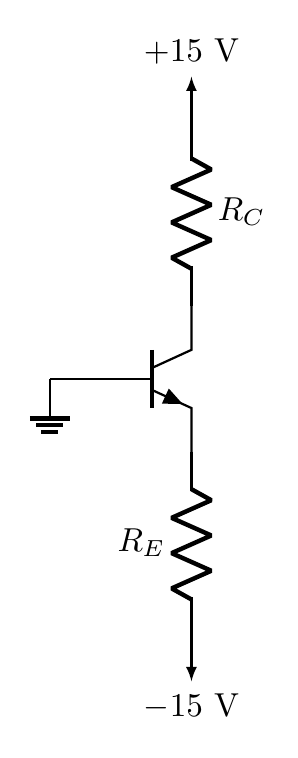
\begin{tikzpicture}[thick,scale=1.2, transform shape]
        
        % Central NPN Transistor
        \node[npn] (Q) at (0,0) {};
        
        % Base connected to ground 
        % (Extended further left to -1.5 to prevent ground symbol overlapping with R_E)
        \draw (Q.B) -- (-1.5, 0) node[ground]{};
        
        % Collector resistor (R_C) and +15V rail
        % (Given more vertical space)
        \draw (Q.C) -- (0, 1.0) to[R, l_=$R_C$] (0, 2.5);
        \draw[-latex] (0, 2.5) -- (0, 3.2) node[above] {$+15\text{ V}$};
        
        % Emitter resistor (R_E) and -15V rail
        % (Given more vertical space)
        \draw (Q.E) -- (0, -1.0) to[R, l_=$R_E$] (0, -2.5);
        \draw[-latex] (0, -2.5) -- (0, -3.2) node[below] {$-15\text{ V}$};
        
    \end{tikzpicture}
\end{center}
\mk{20} \yr{EEE 263 | L-2/T-1 | 2020--21}

\item Design the circuit shown to provide $I_C=3\,\text{mA}$ and $V_{CE}=1.5\,\text{V}$ for $\beta=90$. Use $V_{CC}=3\,\text{V}$ and a current through $R_2$ equal to the base current.
\begin{center}
      \begin{circuitikz}[thick,scale=1.2, transform shape]
        
        % ==========================================
        % Transistor Q
        % ==========================================
        \node[npn] (Q) at (3, 0) {};
        
        % ==========================================
        % Emitter Circuit
        % ==========================================
        \draw (Q.E) -- ++(0, -0.5) node[ground] {};
        
        % ==========================================
        % Collector Stage & Vcc
        % ==========================================
        % Define the collector junction node
        \coordinate (Vc) at (3, 1.5);
        \draw (Q.C) -- (Vc);
        
        % Vcc and Rc
        \draw (Vc) to[R, l=$R_C$] (3, 3.5) coordinate (Vcc);
        \draw[-latex] (Vcc) -- (3, 4) node[right] {$V_{CC}$};
        
        % Output Vc terminal
        \draw (Vc) -- ++(1, 0) node[ocirc] {} node[right] {$V_C$};
        \node[circ] at (Vc) {};
        
        % Current Ic Arrow
        \draw[-latex] (3.3, 1.2) -- (3.3, 0.5) node[midway, right] {$I_C$};
        
        % ==========================================
        % Base & Feedback Network
        % ==========================================
        % Base Junction Node
        \coordinate (B_node) at (1, 0);
        \draw (Q.B) -- (B_node);
        \node[circ] at (B_node) {};
        
        % R1 (Feedback Resistor from Collector)
        \coordinate (R1_top) at (1, 1.5);
        \draw (Vc) -- (R1_top);
        \draw (R1_top) to[R, l_=$R_1$] (B_node);
        
        % R2 to Ground
        \draw (B_node) to[R, l_=$R_2$] (1, -2) node[ground] {};
        
        % ==========================================
        % Caption
        % ==========================================

    \end{circuitikz}
\end{center}
\mk{15} \yr{EEE 263 | L-2/T-1 | 2016--17}    

\end{enumerate}

%%──────────────────────────────────────────────────────────────────────
\subtopic{cA}{Linear Amplifier Constraints}
\label{sub:s2-linear}

\begin{enumerate}\item For the figure shown, find out the maximum collector current that the device can support. If the operating point is set for that maximum current, what kind of problem will we face if we want to use the device as a linear amplifier?


\begin{center}
\begin{tikzpicture}[thick, scale=1.2]
    
    % X and Y Axes
    \draw[->, very thick] (0,0) -- (6,0) node[right] {$V_{CE}(\text{V})$};
    \draw[->, very thick] (0,0) -- (0,4) node[above] {$I_C(\text{mA})$};
    
    % Load line drawing (from y=3 to x=4 for a balanced look)
    \draw[very thick] (0,3) -- (4,0);
    
    % Node labels for intersection points
    \node[left] at (0,3) {$8$};
    \node[below] at (4,0) {$20$};
    
    % "load line" text and pointing arrow
    \draw[-stealth] (2.5, 1.5) -- (1.6, 1.8);
    \node[right] at (2.5, 1.4) {load line};
    
\end{tikzpicture}
\end{center}

\mk{12} \yr{EEE 263 | L-2/T-1 | 2011--12}

\end{enumerate}


%% ══════════════════════════════════════════════════════════════════════
%%  SECTION 3: MOSFET CHARACTERISTICS
%% ══════════════════════════════════════════════════════════════════════
\secdivider{S3 --- MOSFET Characteristics}{Structure, threshold voltage, DC analysis, biasing stability, CMOS logic}{cA}

\markboth{S3: MOSFET Characteristics}{S3: MOSFET Characteristics}
\label{sec:S3}
\section*{S3 \quad MOSFET Characteristics}
\addcontentsline{toc}{section}{S3: MOSFET Characteristics}

%%──────────────────────────────────────────────────────────────────────
\subtopic{cA}{Device Characteristics}
\label{sub:s3-devchar}

\begin{enumerate}\item Explain the different operation regions of an enhancement PMOS transistor with properly labeled $I_D$--$V_{SD}$ plots. Derive the threshold conditions for operating in those regions.
\mk{8} \yr{EEE 263 | L-2/T-1 | 2024--25}

\item For a particular MOSFET operating in the saturation region at a constant $v_{gs}$, $i_D=2\,\text{mA}$ at $v_{ds}=4\,\text{V}$. The $i_D$ increases by 10\% when $v_{ds}$ is doubled. Find the corresponding values of $r_0$, $V_A$, and $\lambda$.
\mk{10} \yr{EEE 263 | L-2/T-1 | 2023--24}

\item Briefly explain the I-V characteristics of an n-channel enhancement MOSFET with necessary plots.
\mk{7} \yr{EEE 263 | L-2/T-1 | 2022--23}

\item What is the difference between enhancement-type and depletion-type MOSFETs? Draw $I_D$ vs.\ $V_{GS}$ and $I_D$ vs.\ $V_{DS}$ characteristics for different values of $V_{GS}$ for both enhancement-type and depletion-type MOSFETs.
\mk{26} \yr{EEE 263 | L-2/T-1 | 2018--19}

\item Showing different operating regions, describe the output characteristics of a MOSFET. Why does current saturation occur in a MOSFET as $V_{DS}$ is increased?
\mk{18} \yr{EEE 263 | L-2/T-1 | Jan--2021}

\end{enumerate}

%%──────────────────────────────────────────────────────────────────────
\subtopic{cA}{Comparison with BJT}
\label{sub:s3-compare}

\begin{enumerate}\item Compare MOSFET and BJT in terms of their operating principles. Mention each of their advantages and disadvantages.
\mk{10} \yr{EEE 263 | L-2/T-1 | 2013--14}

\item What are the mutual advantages and disadvantages of BJT and MOSFET?
\mk{12} \yr{EEE 263 | L-2/T-1 | 2012--13}

\end{enumerate}

%%──────────────────────────────────────────────────────────────────────
\subtopic{cA}{Threshold Voltage}
\label{sub:s3-threshold}

\begin{enumerate}\item Explain the concept of threshold voltage ($V_t$) of a MOSFET. What happens to $V_t$ and oxide capacitance ($C_{ox}$) if: (i) the dielectric thickness is increased/decreased? (ii) the gate insulator is replaced with a more high-$k$ dielectric of the same thickness?
\mk{20} \yr{EEE 263 | L-2/T-1 | 2012--13}

\end{enumerate}

%%──────────────────────────────────────────────────────────────────────
\subtopic{cA}{DC Analysis \& Transistor Sizing}
\label{sub:s3-dc}

\begin{enumerate}\item In the circuit shown, the aspect ratios of $Q_1$ and $Q_2$ are $(W/L)_1 = 2(W/L)_2 = 20$. Both transistors have $V_t=1\,\text{V}$ and $\mu_n C_{ox}=100\,\mu\text{A/V}^2$. Find the node voltages $V_1$, $V_2$, and $V_3$.
\begin{center}
    
\begin{circuitikz}[american, line width=0.8pt]
  \ctikzset{tripoles/mos style/arrows}

    % --- Transistors with increased spacing ---
    \node[nmos] (Q1) at (-3, 2) {};
    \node[nmos, xscale=-1] (Q2) at (3, 2) {};
    
    % Transistor Labels (placed safely inside the wide gap)
    \node at (-2.2, 2) {$Q_1$};
    \node at (2.2, 2) {$Q_2$};

    % --- Common Source Connection ---
    \draw (Q1.S) -- (-3, 0.5) -- (3, 0.5) -- (Q2.S);
    
    % Drop down to V3 and Current Source
    \draw (0, 0.5) -- (0, 0);
    
    % V3 Node (spaced out to the right)
    \draw (0,0) to[short, *-o] (1.5, 0) node[right] {$V_3$};
    
    % Tail Current Source (made longer to avoid clutter)
    \draw (0,0) to[isource, l_=$200\ \mu\text{A}$] (0, -2.5);
    \draw[-latex] (0, -2.5) -- (0, -3.5);

    % --- Left Side (Q1) ---
    % Gate connection
    \draw (Q1.G) to[short, -o] (-4.5, 2|-Q1.G);
    \draw (-4.6, 2|-Q1.G) -- (-5.5, 2|-Q1.G) node[ground] {};
    
    % Drain and V1
    \draw (Q1.D) -- (-3, 3.5);
    \draw (-3, 3.5) to[short, *-o] (-4.5, 3.5) node[left] {$V_1$};
    
    % Resistor and VDD
    \draw (-3, 3.5) to[R, l=$40\text{ k}\Omega$] (-3, 6.5);
    \draw[-latex] (-3, 6.5) -- (-3, 7.5) node[above] {\textbf{+5 V}};


    % --- Right Side (Q2) ---
    % Gate connection
    \draw (Q2.G) to[short, -o] (4.5, 2|-Q2.G);
    \draw (4.6, 2|-Q2.G) -- (5.5, 2|-Q2.G) node[ground] {};
    
    % Drain and V2
    \draw (Q2.D) -- (3, 3.5);
    \draw (3, 3.5) to[short, *-o] (4.5, 3.5) node[right] {$V_2$};
    
    % Resistor and VDD
    \draw (3, 3.5) to[R, l_=$40\text{ k}\Omega$] (3, 6.5);
    \draw[-latex] (3, 6.5) -- (3, 7.5) node[above] {\textbf{+5 V}};

\end{circuitikz}
\end{center}
\mk{17} \yr{EEE 263 | L-2/T-1 | 2024--25}

\item The NMOS transistors in the circuit have $V_t=1\,\text{V}$, $\mu_n C_{ox}=120\,\mu\text{A/V}^2$, $\lambda=0$, and $L_1=L_2=1\,\mu\text{m}$. Find the required values of gate width $W_1$ and $W_2$ for $Q_1$ and $Q_2$, and the value of $R$, for obtaining the voltage values indicated. The current in $R$ will be $120\,\mu\text{A}$.
\begin{center}
    
    \begin{circuitikz}[american, thick]
        \ctikzset{tripoles/mos style/arrows}

        % Q2 Transistor
        \node[nmos] (Q2) at (0, 0) {};
        \node at (0.8, 0) {Q2};
        
        % Q1 Transistor
        \node[nmos] (Q1) at (0, 2.5) {};
        \node at (0.8, 2.5) {Q1};
        
        % Connect Q1 Source to Q2 Drain
        \draw (Q1.S) -- (Q2.D);
        
        % Ground Q2 Source
        \draw (Q2.S) node[ground] {};
        
        % Diode connections (Gate shorted to Drain)
        \draw (Q1.G) -- ++(-0.5, 0) coordinate(g1);
        \draw (g1) |- (Q1.D);
        
        \draw (Q2.G) -- ++(-0.5, 0) coordinate(g2);
        \draw (g2) |- (Q2.D);
        
        % Output nodes
        \draw (Q1.D) to[short, *-o] ++(1.5, 0) node[right] {$+3.5\text{ V}$};
        \draw (Q2.D) to[short, *-o] ++(1.5, 0) node[right] {$+1.5\text{ V}$};
        
        % Resistor and Vdd
        \draw (Q1.D) to[R, l=$R$] ++(0, 2) coordinate(vcc);
        
        % Top +5V Power Terminal (Hollow Triangle pointing up)
        \draw (vcc) -- ++(-0.2, 0) -- ++(0.2, 0.3) -- ++(0.2, -0.3) -- cycle;
        \node[left] at ([xshift=-0.1cm, yshift=0.15cm]vcc) {$+5\text{V}$}; 
        
        % Current indicator (Hollow block arrow pointing down)
        % Coordinates are manually mapped beside the resistor
        \draw[thick] (0.6, 4.6) -- (0.8, 4.6) -- (0.8, 4.1) -- (0.9, 4.1) 
                     -- (0.7, 3.7) -- (0.5, 4.1) -- (0.6, 4.1) -- cycle;
        \node[right] at (1.0, 4.15) {$120\,\mu\text{A}$};
        
    \end{circuitikz}
\end{center}
\mk{15} \yr{EEE 263 | L-2/T-1 | 2023--24}

\item The PMOS transistor in the circuit shown has $V_t=-0.7\,\text{V}$, $\mu_p C_{ox}=60\,\mu\text{A/V}^2$, $L=0.8\,\mu\text{m}$, and $\lambda=0$. Find the value of $W$ and $R$ in order to establish a drain current of $115\,\mu\text{A}$ and a voltage $V_D=3.5\,\text{V}$.
\begin{center}
        \begin{circuitikz}[american, thick]
          \ctikzset{tripoles/mos style/arrows}

        % +5V Power Terminal (Hollow Triangle pointing up)
        \draw (0, 3) coordinate(vcc) -- ++(-0.2, 0) -- ++(0.2, 0.3) -- ++(0.2, -0.3) -- cycle;
        \node[left] at ([xshift=-0.1cm, yshift=0.15cm]vcc) {$+5\text{V}$}; 
        
        % P-channel MOSFET (PMOS)
        % Place PMOS with source (top) connected to Vdd
        \draw (vcc) -- ++(0, -0.5) node[pmos, anchor=S] (M1) {};
        
        % Diode-connection (Gate shorted to Drain)
        \draw (M1.G) -- ++(-0.5, 0) coordinate(gate_short) |- (M1.D);
        
        % Output voltage node VD
        \draw (M1.D) to[short, -o] ++(1.5, 0) node[right] {$V_D$};
        
        % Resistor R connected to Drain
        \draw (M1.D) -- ++(0, -0.5) coordinate(res_top);
        \draw (res_top) to[R, l=$R$] ++(0, -2) node[ground] {};
        
    \end{circuitikz}
\end{center}
\mk{15} \yr{EEE 263 | L-2/T-1 | 2023--24}

\item The NMOS and PMOS transistors in the circuit are matched with $k_n=k_p=1\,\text{mA/V}^2$ and $V_{tn}=-V_{tp}=1\,\text{V}$. Assuming $\lambda=0$ for both MOSFETs, find the drain currents $i_{DN}$ and $i_{DP}$ and the voltage $v_0$ for $v_1=0\,\text{V}$ and $v_1=+2.5\,\text{V}$.


\begin{center}
      \begin{circuitikz}[thick,scale=1.2, transform shape]
        \ctikzset{tripoles/mos style/arrows}


        \node[nmos] (Qn) at (2, 1.5) {};
        \node[left] at (1.1, 1.5) {$Q_N$};
        
         \node[pmos] (Qp) at (2, -1.5) {};
        \node[left] at (1.1, -1.5) {$Q_P$};
        \draw (0,0) node[ocirc]{} node[left]{$V_i$} -- (1,0);
        \draw (1,0) |- (Qn.G);
        \draw (1,0) |- (Qp.G);
        

        \draw[->, >=stealth] (Qn.D) -- ++(0, 0.6) node[above] {$+2.5\mathrm{V}$};
        \draw[->, >=stealth] (Qp.D) -- ++(0, -0.6) node[below] {$-2.5\mathrm{V}$};
  
        \draw (Qn.S) -- (Qp.S);

        \coordinate (Mid) at (2,0);
        \draw (Mid) -- (4.5,0) node[ocirc]{} node[above]{$V_o$};
        
        % 10K লোড রেজিস্টর (আউটপুট থেকে গ্রাউন্ড)
        \draw (3.5,0) node[circ]{} to[R, l={$10\mathrm{K}$}] (3.5,-2) node[ground]{};
        
        % ৫. কারেন্ট অ্যারো (i_DN এবং i_DP)
        % QN-এর সোর্স থেকে নিচের দিকে i_DN
        \draw[->, >=stealth] (2.4, 1.0) -- (2.4, 0.3) node[midway, right] {$i_{DN}$};
        % আউটপুট জাংশন থেকে QP-এর সোর্সের দিকে i_DP
        \draw[->, >=stealth] (2.4, -0.3) -- (2.4, -1.0) node[midway, right] {$i_{DP}$};
        
    \end{circuitikz}
\end{center}

\mk{20} \yr{EEE 263 | L-2/T-1 | 2022--23}


\item For the circuit shown, find the node voltages $V_3$, $V_4$, and $V_5$. The NMOS transistors have $V_t=0.9\,\text{V}$ and $k_n'(W/L)=1.5\,\text{mA/V}^2$.
\begin{center}
    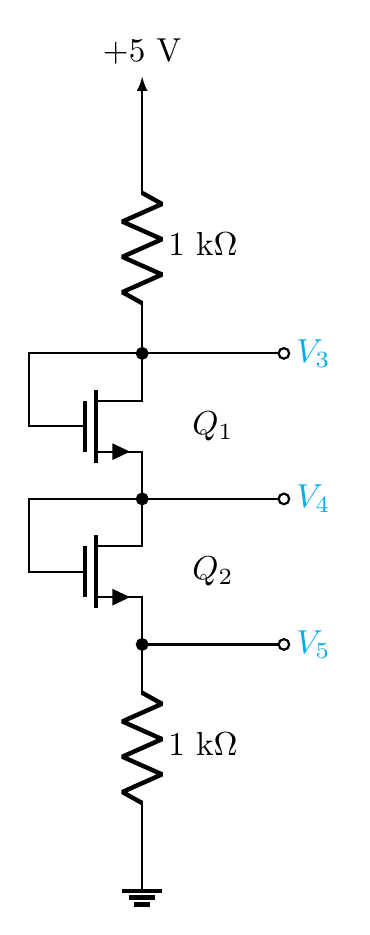
\begin{tikzpicture}[thick,scale=1.2, transform shape]
        \ctikzset{tripoles/mos style/arrows}

        
        % 1. Transistor Q1
        \node[nmos] (Q1) at (0, 2) {};
        \node[right=0.4cm] at (Q1.center) {$Q_1$};
        
        % 2. Transistor Q2 positioned directly below Q1
        % Anchoring Q2's Drain exactly at Q1's Source creates a seamless junction
        \node[nmos, anchor=D] (Q2) at (Q1.S) {};
        \node[right=0.4cm] at (Q2.center) {$Q_2$};
        
        % 3. Top Power Rail and Top Resistor
        % Drawing downwards places the "1 k\Omega" label on the right side
        \draw (0, 5) to[R, l=$1\text{ k}\Omega$] (Q1.D);
        \draw[-latex] (0, 5) -- (0, 5.7) node[above] {$+5\text{ V}$};
        
        % 4. Bottom Resistor and Ground
        \draw (Q2.S) to[R, l=$1\text{ k}\Omega$] (0, -2.5) node[ground]{};
        
        % 5. V3 Node and Diode Connection (Gate to Drain on Q1)
        \draw (Q1.D) node[circ]{} -- ++(1.5,0) node[ocirc]{} node[right, text=cyan] {$V_3$};
        \draw (Q1.D) -- ++(-1.2,0) |- (Q1.G);
        
        % 6. V4 Node and Diode Connection (Gate to Drain on Q2)
        \draw (Q1.S) node[circ]{} -- ++(1.5,0) node[ocirc]{} node[right, text=cyan] {$V_4$};
        \draw (Q1.S) -- ++(-1.2,0) |- (Q2.G);
        
        % 7. V5 Node
        \draw (Q2.S) node[circ]{} -- ++(1.5,0) node[ocirc]{} node[right, text=cyan] {$V_5$};
        
    \end{tikzpicture}
\end{center}
\mk{28} \yr{EEE 263 | L-2/T-1 | Jan--2021}

\item For the circuit shown, find $R$ so that $I_{D1}=0.4\,\text{mA}$. Also find $V_{D1}$, $V_{D2}$, and $I_{D2}$. $Q_1$ and $Q_2$ are identical. Given: $V_t=2\,\text{V}$, $\mu_n C_{ox}=20\,\mu\text{A/V}^2$, $L=10\,\mu\text{m}$, $W=100\,\mu\text{m}$.
\begin{center}
    \begin{circuitikz}[thick,american, scale=1.3]
          \ctikzset{tripoles/mos style/arrows}

    % 1. Left Transistor Q2 (Flipped horizontally so gate faces right)
    \node[nmos, xscale=-1] (Q2) at (0,0) {};
    \node[left=4pt] at (Q2.center) {$Q_2$};
    \draw (Q2.source) -- ++(0,-0.4) node[ground] {};
    
    % 2. Right Transistor Q1 (Standard orientation, gate faces left)
    \node[nmos] (Q1) at (3,0) {};
    \node[right=4pt] at (Q1.center) {$Q_1$};
    \draw (Q1.source) -- ++(0,-0.4) node[ground] {};

    % 3. Connect Gates together
    \draw (Q2.gate) -- (Q1.gate);
    
    % 4. Left Drain Branch (Q2) with Resistor and Power Rail
    \draw (Q2.drain) -- ++(0,0.4) coordinate (D2_node)
          to[R, l=$10\text{ k}\Omega$] ++(0,1.6) coordinate (Vcc2);
    \draw[->, >=stealth, thick] (Vcc2) -- ++(0,0.5) node[above] {$+10\text{V}$};
    \fill (D2_node) circle (1.5pt) node[right=3pt] {$D_2$};
    
    % 5. Right Drain Branch (Q1) with Resistor and Power Rail
    \draw (Q1.drain) -- ++(0,0.4) coordinate (D1_node)
          to[R, l_=$R$] ++(0,1.6) coordinate (Vcc1);
    \draw[->, >=stealth, thick] (Vcc1) -- ++(0,0.5) node[above] {$+10\text{V}$};
    \fill (D1_node) circle (1.5pt) node[right=3pt] {$D_1$};

    % 6. Diode-Connection Wire from the Gate Line to Drain D1
    \coordinate (gate_conn) at (1.4, 0);
    \fill (gate_conn) circle (1.5pt);
    \draw (gate_conn) |- (D1_node);

    % 7. External Current Arrows (Matching handwritten style)
    % Left branch current (ID2)
    \draw[->, >=stealth, thick] (-0.7, 1.6) -- (-0.7, 0.9);
    \node[left] at (-0.7, 1.45) {$I_{D2}$};
    
    % Right branch current (ID1)
    \draw[->, >=stealth, thick] (4.1, 1.8) -- (4.1, 1.1);
    \node[right] at (4.1, 1.45) {$I_{D1} = 0.4\text{ mA}$};

    % 8. Figure Caption

\end{circuitikz}
\end{center}
\mk{20} \yr{EEE 263 | L-2/T-1 | 2018--19}

\item For the circuit shown, for all MOSFETs $|V_t|=1\,\text{V}$, $\mu_n C_{ox}=50\,\mu\text{A/V}^2$, $L=1\,\mu\text{m}$, $W=10\,\mu\text{m}$. Find $V$ and $I$. If $Q_3$ and $Q_4$ are made to have $W=100\,\mu\text{m}$, find $V$ and $I$ in that case.
\begin{center}
      \begin{circuitikz}[thick,scale=1.2, transform shape]
          \ctikzset{tripoles/mos style/arrows}

        % ==========================================
        % Transistors
        % ==========================================
        % Q3 (Bottom Left, NMOS, reversed so gate is on right)
        \node[nmos, xscale=-1] (Q3) at (0, 0) {};
        \node at (-0.8, 0) {$Q_3$};
        
        % Q1 (Bottom Right, NMOS, standard)
        \node[nmos] (Q1) at (3, 0) {};
        \node at (3.8, 0) {$Q_1$};
        
        % Q4 (Top Left, NMOS, standard)
        \node[nmos] (Q4) at (0, 3) {};
        \node at (0.8, 3) {$Q_4$};
        
        % Q2 (Top Right, NMOS, reversed so gate is on right)
        \node[nmos, xscale=-1] (Q2) at (3, 3) {};
        \node at (2.2, 3) {$Q_2$};

        % ==========================================
        % Source Connections & Grounds
        % ==========================================
        % Grounding NMOS Sources
        \draw (Q3.S) -- ++(0, -0.3) node[ground] {};
        \draw (Q1.S) -- ++(0, -0.3) node[ground] {};
        
        % ==========================================
        % Middle Connections & Output
        % ==========================================
        % Left side connections (Top Source to Bottom Drain)
        \draw (Q4.S) -- (Q3.D) coordinate[midway] (Vo_node);
        
        % Right side connections (Top Source to Bottom Drain)
        \draw (Q2.S) -- (Q1.D) coordinate[midway] (D_mid);
        
        % Output Vo terminal
        \draw (Vo_node) -- ++(-1, 0) node[ocirc] {} node[left] {$V_o$};
        \node[circ] at (Vo_node) {};
        
        % Current Arrow I (next to Q4 drain)
        \draw[-latex] (0.3, 2.3) -- (0.3, 1.5) node[midway, right] {$I$};

        % ==========================================
        % Gate Connections & Feedback Loop
        % ==========================================
        % Gate connection between Q3 and Q1
        \draw (Q3.G) -- (Q1.G) coordinate[midway] (G_mid);
        \node[circ] at (G_mid) {};
        
        % Diode-connected feedback trace (up then right to drain line)
        \node[circ] at (D_mid) {};
        \draw (G_mid) |- (D_mid);
        
        % ==========================================
        % Top +5V Bias Connections
        % ==========================================
        % Q4 Drain and Gate paths
        \draw (Q4.G) -- ++(-0.6, 0) coordinate (Q4g);
        \draw[-latex] (Q4g) -- (Q4g |- 0, 4.5);
        \draw[-latex] (Q4.D) -- (Q4.D |- 0, 4.5);
        \node at (-0.3, 4.7) {$+5V$};
        
        % Q2 Drain and Gate paths
        \draw (Q2.G) -- ++(0.6, 0) coordinate (Q2g);
        \draw[-latex] (Q2g) -- (Q2g |- 0, 4.5);
        \draw[-latex] (Q2.D) -- (Q2.D |- 0, 4.5);
        \node at (3.3, 4.7) {$+5V$};

        % ==========================================
        % Caption
        % ==========================================

    \end{circuitikz}
\end{center}
\mk{26} \yr{EEE 263 | L-2/T-1 | 2016--17}

\item The NMOS and PMOS transistors in the circuit shown have $k_n(W/L)=k_p(W/L)=1\,\text{mA/V}^2$ and $V_{tn}=-V_{tp}=1\,\text{V}$. Assume $\lambda=0$. Find $i_{DN}$, $i_{DP}$, and $v_o$ for $V_i=+2.5\,\text{V}$ and $V_i=-2.5\,\text{V}$.

\begin{center}
      \begin{circuitikz}[thick,scale=1.2, transform shape]
        \ctikzset{tripoles/mos style/arrows}

        % ===================================================
        % CMOS / Class-B Push-Pull Output Stage
        % ===================================================
        
        % ১. ট্রানজিস্টর প্লেসমেন্ট 
        % QN (NMOS): ড্রেইন উপরে, সোর্স নিচে (বাইরের দিকে তীর)
        \node[nmos] (Qn) at (2, 1.5) {};
        \node[left] at (1.1, 1.5) {$Q_N$};
        
        % QP (PMOS): সোর্স উপরে (ভেতরের দিকে তীর), ড্রেইন নিচে
        % (এটি ডিফল্ট ওরিয়েন্টেশন, যা আপনার ছবির সাথে পুরোপুরি মিলে যায়)
        \node[pmos] (Qp) at (2, -1.5) {};
        \node[left] at (1.1, -1.5) {$Q_P$};
        
        % ২. ইনপুট সেকশন (V_i)
        \draw (0,0) node[ocirc]{} node[left]{$V_i$} -- (1,0);
        \draw (1,0) |- (Qn.G);
        \draw (1,0) |- (Qp.G);
        
        % ৩. পাওয়ার সাপ্লাই কানেকশন
        % QN এর ড্রেইন থেকে +2.5V
        \draw[->, >=stealth] (Qn.D) -- ++(0, 0.6) node[above] {$+2.5\mathrm{V}$};
        % QP এর ড্রেইন থেকে -2.5V
        \draw[->, >=stealth] (Qp.D) -- ++(0, -0.6) node[below] {$-2.5\mathrm{V}$};
        
        % ৪. আউটপুট সেকশন (V_o)
        % উভয়ের সোর্স একসাথে যুক্ত করা
        \draw (Qn.S) -- (Qp.S);
        
        % মাঝখানের জাংশন থেকে আউটপুট নোড
        \coordinate (Mid) at (2,0);
        \draw (Mid) -- (4.5,0) node[ocirc]{} node[above]{$V_o$};
        
        % 10K লোড রেজিস্টর (আউটপুট থেকে গ্রাউন্ড)
        \draw (3.5,0) node[circ]{} to[R, l={$10\mathrm{K}$}] (3.5,-2) node[ground]{};
        
        % ৫. কারেন্ট অ্যারো (i_DN এবং i_DP)
        % QN-এর সোর্স থেকে নিচের দিকে i_DN
        \draw[->, >=stealth] (2.3, 1.0) -- (2.3, 0.3) node[midway, right] {$i_{DN}$};
        % আউটপুট জাংশন থেকে QP-এর সোর্সের দিকে i_DP
        \draw[->, >=stealth] (2.3, -0.3) -- (2.3, -1.0) node[midway, right] {$i_{DP}$};
        
    \end{circuitikz}
\end{center}

\mk{20} \yr{EEE 263 | L-2/T-1 | 2014--15}

\item The NMOS transistors in the circuit have $V_t=1\,\text{V}$, $\mu_n C_{ox}=120\,\mu\text{A/V}^2$, $L_1=L_2=1\,\mu\text{m}$. Find $W_1$, $W_2$, and $R$, where $W_1$ and $W_2$ are the gate widths of Q1 and Q2 respectively.
\begin{center}
    \begin{circuitikz}[thick,scale=1.2, transform shape]
                    \ctikzset{tripoles/mos style/arrows}

        % ===================================================
        % Diode-Connected NMOS Circuit
        % ===================================================
        
        % ১. ট্রানজিস্টর প্লেসমেন্ট 
        % Q1 (NMOS): নিচে
        \node[nmos] (Q1) at (0, 0) {};
        \node[right] at (0.6, -0.3) {$Q_1$}; % লেবেল পজিশনিং
        
        % Q2 (NMOS): উপরে
        \node[nmos] (Q2) at (0, 2.5) {};
        \node[right] at (0.6, 2.2) {$Q_2$}; % লেবেল পজিশনিং
        
        % ২. সোর্স এবং ড্রেইন কানেকশন
        % Q1-এর সোর্স গ্রাউন্ডে যুক্ত
        \draw (Q1.S) node[ground]{};
        
        % Q1-এর ড্রেইন থেকে Q2-এর সোর্সে সংযোগ
        \draw (Q1.D) -- (Q2.S);
        
        % ৩. ডায়োড কানেকশন (Gate to Drain short)
        % Q1-এর জন্য (বাম দিক দিয়ে ঘুরিয়ে গেইটে যুক্ত)
        \draw (Q1.D) -- ++(-1.2, 0) |- (Q1.G);
        
        % Q2-এর জন্য (বাম দিক দিয়ে ঘুরিয়ে গেইটে যুক্ত)
        \draw (Q2.D) -- ++(-1.2, 0) |- (Q2.G);
        
        % ৪. রেজিস্টর (R) এবং +5V সাপ্লাই
        \draw (Q2.D) to[R, l_=$R$] ++(0, 1.8) coordinate (Vdd);
        \draw[->, >=stealth] (Vdd) -- ++(0, 0.6) node[right] {$+5\mathrm{V}$};
        
        % ৫. আউটপুট টার্মিনাল নোডসমূহ
        % Q2-এর ড্রেইন থেকে +3.5V
        \draw (Q2.D) node[circ]{} -- ++(1.5, 0) node[ocirc]{} node[right]{$+3.5\mathrm{V}$};
        
        % Q1-এর ড্রেইন (বা Q2-এর সোর্স) থেকে +1.5V
        \draw (Q1.D) node[circ]{} -- ++(1.5, 0) node[ocirc]{} node[right]{$+1.5\mathrm{V}$};
        
        % ৬. কারেন্ট ডিরেকশন অ্যারো (I = 120\muA)
        % রেজিস্টরের বাম পাশে, নিচের দিকে তীর
        \draw[->, >=stealth] (-1.0, 4.8) -- (-1.0, 3.6) node[midway, left] {$I = 120\mu\mathrm{A}$};
        
    \end{circuitikz}
\end{center}
\mk{16} \yr{EEE 263 | L-2/T-1 | 2014--15}

\item For the circuit shown, find the value of $V_0$. Both NMOS transistors have $V_t=1\,\text{V}$, $\lambda=0$, and $\mu_n C_{ox}(W/L)=1\,\text{mA/V}^2$. Supply voltage is 5\,V.


\begin{center}
  \begin{circuitikz}[thick,scale=1.2, transform shape]
          \ctikzset{tripoles/mos style/arrows}

        % ===================================================
        % Place the two NMOS Transistors
        % ===================================================
        \node[nmos] (M1) at (0,0) {};
        \node[nmos] (M2) at (3,0) {};
        
        % ===================================================
        % M1 (Left NMOS) Connections
        % ===================================================
        % Gate input (2V)
        \draw (M1.G) -- ++(-1, 0) node[left] {$2\text{V}$};
        
        % Drain to 1K Resistor (Label on left) and connected to M2 Gate
        \draw (M1.D) node[circ]{} to[R, l=$1\text{K}$] ++(0, 2) coordinate (Top1);
        \draw (M1.D) -| (M2.G); % Draws a right-angled line to M2's Gate
        
        % ===================================================
        % M2 (Right NMOS) Connections
        % ===================================================
        % Drain to 1K Resistor (Label on right) and Output V0
        \draw (M2.D) node[circ]{} to[R, l_=$1\text{K}$] ++(0, 2) coordinate (Top2);
        \draw (M2.D) to[short, -o] ++(1.2, 0) node[right] {$V_0$};
        
        % ===================================================
        % Top (VDD) Connections
        % ===================================================
        % Connect the top of both resistors and draw the 5V upward arrow
        \draw (Top1) -- (Top2) coordinate[midway] (Vdd_mid);
        \draw[->, >=stealth] (Vdd_mid) -- ++(0, 0.6) node[right] {$5\text{V}$};
        
        % ===================================================
        % Bottom (Ground) Connections
        % ===================================================
        % Connect the sources of both NMOS and draw the downward arrow (0)
        \draw (M1.S) -- (M1.S |- 0, -1.2) coordinate (Bot1);
        \draw (M2.S) -- (M2.S |- 0, -1.2) coordinate (Bot2);
        
        \draw (Bot1) -- (Bot2) coordinate[midway] (Gnd_mid);
        \draw[->, >=stealth] (Gnd_mid) -- ++(0, -0.6) node[right] {$0$};
        
    \end{circuitikz}
\end{center}

\mk{16} \yr{EEE 263 | L-2/T-1 | 2013--14}

\item The NMOS transistors in the circuit have $V_t=1\,\text{V}$, $\mu_n C_{ox}=120\,\mu\text{A/V}^2$, and $L_1=L_2=L_3=1\,\mu\text{m}$. Find the required values of gate width for each of Q1, Q2, and Q3 to obtain the voltage and current values indicated in the figure.

\begin{center}
      \begin{circuitikz}[thick,american, thick, scale=1.3, transform shape]
\ctikzset{tripoles/mos style/arrows}
        % ===================================================
        % 1. Start from Ground at the very bottom
        % ===================================================
        \node[ground] (GND) at (0, 0) {};


        % ===================================================
        % 2. Place NMOS Q1 (Bottom Transistor)
        % Using standard 'nmos' 
        % ===================================================
        \node[nmos, anchor=source] (Q1) at (0, 1) {$Q_1$};
        % Connect source to ground
        \draw (Q1.source) -- (GND);
        
        % Diode connection for Q1: Connect Drain -> Feedback Node -> Gate
        \draw (Q1.drain) -- ++(0, 0.5) coordinate (FB_Q1); 
        \draw (FB_Q1) -- ++(-1.4, 0) |- (Q1.gate);
        \fill (FB_Q1) circle (1.5pt); % Connection Dot

        % Output Node (+1.5V)
        \draw (FB_Q1) to[short, -o] ++(1.4, 0) node[right] {$+1.5\text{V}$};


        % ===================================================
        % 3. Place NMOS Q2 (Middle Transistor)
        % ===================================================
        \node[nmos, anchor=source] (Q2) at (0, 3) {$Q_2$};
        % Connect Source of Q2 to the node between Q2 and Q1
        \draw (Q2.source) -- (FB_Q1);

        % Diode connection for Q2
        \draw (Q2.drain) -- ++(0, 0.5) coordinate (FB_Q2);
        \draw (FB_Q2) -- ++(-1.4, 0) |- (Q2.gate);
        \fill (FB_Q2) circle (1.5pt); % Connection Dot

        % Output Node (+3.5V)
        \draw (FB_Q2) to[short, -o] ++(1.4, 0) node[right] {$+3.5\text{V}$};


        % ===================================================
        % 4. Place NMOS Q3 (Top Transistor)
        % ===================================================
        \node[nmos, anchor=source] (Q3) at (0, 5) {$Q_3$};
        % Connect Source of Q3 to node FB_Q2
        \draw (Q3.source) -- (FB_Q2);
    
        % Diode connection for Q3
        \draw (Q3.drain) -- ++(0, 0.5) coordinate (FB_Q3);
        \draw (FB_Q3) -- ++(-1.4, 0) |- (Q3.gate);
        \fill (FB_Q3) circle (1.5pt); % Connection Dot


        % ===================================================
        % 5. Top Connections: VCC and Current Arrow
        % ===================================================
        % VCC (+5V) with upward arrow
        \draw (FB_Q3) -- ++(0, 0.8) node[above] {$+5\text{V}$};
        
        % Current Measurement (120 uA) downward arrow next to the node
        \draw[->, >=stealth] (0.8, 6.2) -- (0.8, 5.6) node[midway, right] {$120\,\mu\text{A}$};

    \end{circuitikz}
\end{center}

\mk{14} \yr{EEE 263 | L-2/T-1 | 2012--13}

\item Determine all node voltages and drain current of the circuit. Assume $V_t=1\,\text{V}$, $K_n' W/L = 1\,\text{mA/V}^2$, $\lambda=0$, $V_{DD}=+10\,\text{V}$, $R_D=6\,\text{k}\Omega$.

\begin{center}
\begin{circuitikz}[thick,american, thick, scale=1.2, transform shape]
  \ctikzset{tripoles/mos style/arrows}

  % NMOS Transistor
  \draw (3,3) node[nmos] (Q) {};
  
  % ট্রানজিস্টরের Source পিনের উপর ম্যানুয়ালি তীর (Arrow) যুক্ত করা হলো
  
  % Gate connection with a node dot
  \draw (Q.G) -- (0,3);
  \draw[fill=black] (0,3) circle (1.5pt);
  
  % Left side (Gate bias resistors)
  \draw (0,6) to[R, l_={ $R_{G1} = 10\text{ M}\Omega$ }] (0,3)
        to[R, l_={ $R_{G2} = 10\text{ M}\Omega$ }] (0,0);
        
  % Right side (Drain resistor)
  \draw (3,6) to[R, l={ $R_D = 6\text{ k}\Omega$ }] (Q.D);
  
  % Source resistor
  \draw (Q.S) to[R, l={ $R_S = 6\text{ k}\Omega$ }] (3,0);
  
  % Top VDD arrows
  \draw[-stealth] (0,6) -- (0,6.8);
  \draw[-stealth] (3,6) -- (3,6.8);
  
  % VDD Label (Centered at the top)
  \node[above] at (1.5, 6.8) {$V_{DD} = +10\text{ V}$};
  
  % Ground connections
  \draw (0,0) node[ground]{};
  \draw (3,0) node[ground]{};
  
\end{circuitikz}
\end{center}


\mk{20} \yr{EEE 263 | L-2/T-1 | 2011--12}



\end{enumerate}

%%──────────────────────────────────────────────────────────────────────
\subtopic{cA}{Multi-stage MOSFET Circuit Design}
\label{sub:s3-multistage}

\begin{enumerate}\item For the circuit shown with transistor parameters $K_{n1}=500\,\mu\text{A/V}^2$, $K_{n2}=200\,\mu\text{A/V}^2$, $V_{T1}=V_{T2}=1.2\,\text{V}$, design the circuit such that $I_{D1}=0.1\,\text{mA}$, $I_{D2}=0.3\,\text{mA}$, $V_{DS1}=V_{DS2}=5\,\text{V}$.
\begin{center}
  
    \begin{circuitikz}[thick,scale=1.2, transform shape]
        \ctikzset{tripoles/mos style/arrows}

        % ==========================================
        % Top and Bottom Rails
        % ==========================================
        \draw (-2.5, 3) -- (3.5, 3);
        \draw (-2.5, -3) -- (3.5, -3);

        % Power supply arrows
        \draw[-latex] (1.2, 3) -- (1.2, 3.8) node[right] {$+5V$};
        \draw[-latex] (1.2, -3) -- (1.2, -3.8) node[right] {$-5V$};

        % ==========================================
        % Transistors (Both NMOS)
        % ==========================================
        \node[nmos] (M1) at (0, 0) {};
        \node[right] at (M1.text) {$M_1$};
        
        \node[nmos] (M2) at (2.5, 0) {};
        \node[right] at (M2.text) {$M_2$};

        % ==========================================
        % Left Voltage Divider (Gate of M1)
        % ==========================================
        \draw (M1.G) -- ++(-1.5, 0) coordinate (G1);
        \node[circ] at (G1) {};
        \draw (G1) to[R, l=$R_1$] (G1 |- 0, 3);
        \draw (G1) to[R, l=$337\text{ k}\Omega$] (G1 |- 0, -3);
        
        % Nodes on the rails for the divider
        \node[circ] at (G1 |- 0, 3) {};
        \node[circ] at (G1 |- 0, -3) {};

        % ==========================================
        % M1 Drain and Source Branches
        % ==========================================
        % Drain branch
        \draw (M1.D) -- ++(0, 0.5) coordinate (D1);
        \node[circ] at (D1) {};
        \draw (D1) to[R, l_=$R_{D1}$] (D1 |- 0, 3);
        \node[circ] at (D1 |- 0, 3) {};
        
        % Source branch
        \draw (M1.S) to[R, l_=$R_{S1}$] (M1.S |- 0, -3);
        \node[circ] at (M1.S |- 0, -3) {};

        % ==========================================
        % M2 Gate, Drain, and Source Branches
        % ==========================================
        % Gate connection to M1 Drain
        \draw (D1) -- (M2.G);

        % Drain connection (Direct to +5V)
        \draw (M2.D) -- (M2.D |- 0, 3);
        \node[circ] at (M2.D |- 0, 3) {};
        
        % Source branch
        \draw (M2.S) to[R, l_=$R_{S2}$] (M2.S |- 0, -3);
        \node[circ] at (M2.S |- 0, -3) {};

    \end{circuitikz}
\end{center}
\mk{20} \yr{EEE 263 | L-2/T-1 | 2016--17}

\end{enumerate}

%%──────────────────────────────────────────────────────────────────────
\subtopic{cA}{MOSFET Transconductance}
\label{sub:s3-gm}

\begin{enumerate}

\item Derive the condition of small signal operation considering a simple CS nMOS amplifier circuit. Find the expression of MOSFET transconductance $g_m$ from there as well.
\mk{8} \yr{EEE 263 | L-2/T-1 | 2023--24}

    
\item How can the MOSFET transconductance $g_m$ be varied with the design parameters $W/L$ ratio and overdrive voltage $V_{ov}$? Explain.
\mk{10} \yr{EEE 263 | L-2/T-1 | 2014--15}

\end{enumerate}

%%──────────────────────────────────────────────────────────────────────
\subtopic{cA}{Voltage Transfer Characteristics}
\label{sub:s3-vtc}

\begin{enumerate}\item Draw the voltage transfer characteristic of a MOSFET. In which part of this graph is a MOSFET used as an amplifier, and why? What are the benefits and drawbacks of increasing bias voltage?
\mk{19} \yr{EEE 263 | L-2/T-1 | 2012--13}

\end{enumerate}

%%──────────────────────────────────────────────────────────────────────
\subtopic{cA}{MOSFET as Small-Signal Amplifier}
\label{sub:s3-ssa}

\begin{enumerate}\item Briefly explain the operation of a MOSFET as a small-signal amplifier and deduce its VTC from the $I_D$--$V_{DS}$ graph.
\mk{15} \yr{EEE 263 | L-2/T-1 | 2017--18}

\end{enumerate}

%%──────────────────────────────────────────────────────────────────────
\subtopic{cA}{Biasing Stability}
\label{sub:s3-biasing}

\begin{enumerate}\item What is the reason for biasing a MOSFET? Write a short note on the biasing technique of a discrete MOSFET using a fixed voltage at the gate and a resistance $R_s$ in the source.
\mk{11} \yr{EEE 263 | L-2/T-1 | 2017--18}

\item Design the circuit shown to obtain a current $I_D = 80\,\mu\text{A}$. Given: $V_t=0.6\,\text{V}$, $\mu_n C_{ox}=200\,\mu\text{A/V}^2$, $L=0.8\,\mu\text{m}$, $W=4\,\mu\text{m}$, and $V_A=50\,\text{V}$.


\begin{center}
      \begin{circuitikz}[thick,scale=1.5, transform shape]
          \ctikzset{tripoles/mos style/arrows}

        % ===================================================
        % VDD Top Connection
        % ===================================================
        % Upward arrow for VDD
        \draw[->, >=stealth] (0, 2.5) -- (0, 3) node[right] {$V_{DD} = +3\text{V}$};
        
        % Current Arrow (ID) pointing downwards on the left
        \draw[->, >=stealth] (-0.7, 2.5) node[left] {$I_D$} -- (-0.7, 1.8);

        % ===================================================
        % Resistor R
        % ===================================================
        \draw (0, 2.5) to[R, l=$R$] (0, 1) coordinate (drain);

        % ===================================================
        % NMOS Transistor
        % ===================================================
        % Placing the NMOS with its Drain anchored to the resistor
        \node[nmos, anchor=D] (M) at (drain) {};

        % Gate to Drain Short Connection (Diode-connected)
        % Wire goes left, then down, then right to the Gate
        \draw (drain) -- ++(-1.2, 0) |- (M.G);

        % ===================================================
        % Source and Ground
        % ===================================================
        % Source to ground triangle with '0' label
        \draw (M.S) -- ++(0, -0.5) node[ground] {} node[right=0.2cm] {$0$};

    \end{circuitikz}
\end{center}
\mk{16} \yr{EEE 263 | L-2/T-1 | 2013--14}

\item Explain graphically the benefit of using a resistance at the MOSFET source terminal. How does it counteract the problem of unpredictable variation in process parameters such as $V_t$, $C_{ox}$, $\mu_n$?
\mk{20} \yr{EEE 263 | L-2/T-1 | 2012--13}

\end{enumerate}

%%──────────────────────────────────────────────────────────────────────
\subtopic{cA}{CMOS Logic Implementation}
\label{sub:s3-cmos}

\begin{enumerate}\item The diagram shows a Boolean function $Y$ being implemented as a combinational circuit. Design a CMOS transistor-level implementation of the Boolean function using the minimum number of transistors.
\begin{center}
    
    \begin{circuitikz}
        % --- Gate Placement ---
        % Coordinates are carefully chosen so that the standard input offsets 
        % (+/- 0.28 vertically) align perfectly with the horizontal wire runs.
        \node[nor port]  (nor1)  at (4, 4.72) {};
        \node[nand port] (nand1) at (3, 2.00) {};
        \node[nor port]  (nor2)  at (5.5, 3.72) {};
        \node[nor port]  (nor3)  at (7.5, 4.22) {};
        \node[nand port] (nand2) at (9.5, 5.72) {};

        % --- Input Nodes ---
        \node[left] at (0, 6) (A) {A};
        \node[left] at (0, 5) (B) {B};
        \node[left] at (0, 4) (C) {C};

        % --- Input Wiring ---
        % A goes directly to top input of the final NAND gate
        \draw (A) -- (nand2.in 1);

        % B main line goes to top input of top NOR gate
        \draw (B) -- (nor1.in 1);
        % B branches down to top input of bottom-left NAND gate
        \draw (1, 5) to[short, *-] (1, 2.28) -- (nand1.in 1);

        % C main line goes directly to top input of bottom-middle NOR gate
        \draw (C) -- (nor2.in 1);
        % C branches down to bottom input of bottom-left NAND gate
        \draw (1.5, 6) to[short, *-] (1.5, 1.72) -- (nand1.in 2);
        % C branches up to bottom input of top NOR gate
        \draw (2.5, 4) to[short, *-] (2.5, 4.44) -- (nor1.in 2);

        % --- Internal Wiring ---
        % Output of bottom-left NAND to bottom input of bottom-middle NOR
        \draw (nand1.out) |- (nor2.in 2);
        
        % Output of top NOR to top input of middle-right NOR
        \draw (nor1.out) |- (nor3.in 1);
        
        % Output of bottom-middle NOR to bottom input of middle-right NOR
        \draw (nor2.out) |- (nor3.in 2);
        
        % Output of middle-right NOR to bottom input of final NAND
        \draw (nor3.out) |- (nand2.in 2);

        % --- Output Terminal ---
        \draw (nand2.out) -- ++(0.5,0) node[right] {Y};

    \end{circuitikz}
\end{center}
\mk{20} \yr{EEE 263 | L-2/T-1 | 2020--21}

\end{enumerate}

%%──────────────────────────────────────────────────────────────────────
\subtopic{cA}{CMOS Sizing and Delay}
\label{sub:s3-sizing}

\begin{enumerate}
    \item For the logic circuit shown, choose transistor widths to achieve equal rise and fall resistance as a unit inverter. Assume $\mu_n = 3\mu_p$. What is the minimum and maximum propagation delay in the circuit?
\begin{center}
    
    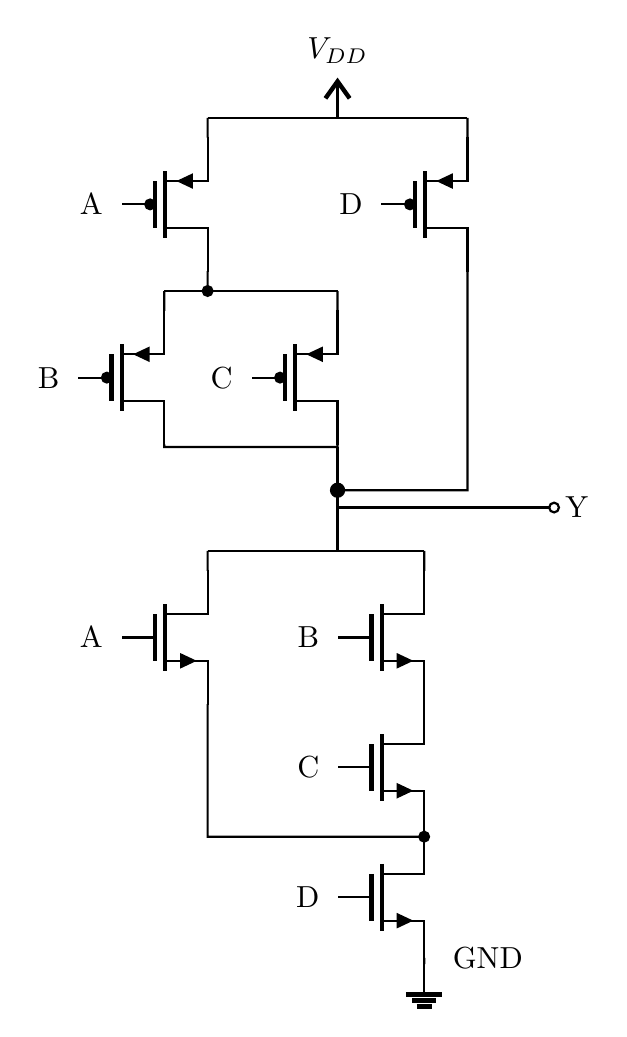
\begin{tikzpicture}[scale=1.1, transform shape, thick]
                  \ctikzset{tripoles/mos style/arrows}

        % ===================================================
        % 1. PULL-UP NETWORK (PMOS)
        % ===================================================
        
        % PMOS A (Top Left)
        \node[pmos] (pA) at (-1, 3.5) {};
        \node[left=0.1cm] at (pA.G) {A};
        
        % PMOS D (Top Right)
        \node[pmos] (pD) at (2, 3.5) {};
        \node[left=0.1cm] at (pD.G) {D};
        
        % PMOS B & C (Middle Parallel Pair)
        \node[pmos] (pB) at (-1.5, 1.5) {};
        \node[left=0.1cm] at (pB.G) {B};
        
        \node[pmos] (pC) at (0.5, 1.5) {};
        \node[left=0.1cm] at (pC.G) {C};
        
        % VDD Top Rail & Independent Source Connection
        \draw (-1, 4.5) -- (2, 4.5);
        \draw (0.5, 4.5) node[vcc] {$V_{DD}$};
        \draw (pA.S) -- (-1, 4.5);
        \draw (pD.S) -- (2, 4.5);
        
        % Connection from A down to B & C split rail
        \draw (pA.D) -- (-1, 2.5) node[circ] {};
        \draw (-1.5, 2.5) -- (0.5, 2.5);
        \draw (-1.5, 2.5) -- (pB.S);
        \draw (0.5, 2.5) -- (pC.S);
        
        % Separate Upper Middle Line: PMOS B & C merging together
        \draw (pB.D) -- (-1.5, 0.7) -- (0.5, 0.7) -- (pC.D);
        \draw (0.5, 0.7) -- (0.5, 0.2); % Drops down to meet the central node
        
        % Separate Side Line: PMOS D wire coming down independently
        \draw (pD.D) -- (2, 0.2) -- (0.5, 0.2);
        
        % ===================================================
        % 2. CENTRAL JUNCTION & OUTPUT TERMINAL (Y)
        % ===================================================
        \fill (0.5, 0.2) circle (2.5pt); % Main central meeting node
        \draw (0.5, 0) -- (3, 0) node[ocirc] {} node[right] {Y};
        
        % ===================================================
        % 3. PULL-DOWN NETWORK (NMOS)
        % ===================================================
        
        % NMOS A (Left branch)
        \node[nmos] (nA) at (-1, -1.5) {};
        \node[left=0.1cm] at (nA.G) {A};
        
        % NMOS B & C Stack (Right branch)
        \node[nmos] (nB) at (1.5, -1.5) {};
        \node[left=0.1cm] at (nB.G) {B};
        
        \node[nmos] (nC) at (1.5, -3.0) {};
        \node[left=0.1cm] at (nC.G) {C};
        
        % NMOS D (Bottom)
        \node[nmos] (nD) at (1.5, -4.5) {};
        \node[left=0.1cm] at (nD.G) {D};
        
        % Separate Lower Middle Line: Connection from central node down to NMOS network
        \draw (0.5, 0.2) -- (0.5, -0.5);
        \draw (-1, -0.5) -- (1.5, -0.5); % NMOS top rail split
        \draw (-1, -0.5) -- (nA.D);
        \draw (1.5, -0.5) -- (nB.D);
        
        % Series connection between NMOS B and C
        \draw (nB.S) -- (nC.D);
        
        % Bottom connection of A and C merging into D
        \draw (nA.S) -- (-1, -3.8) -- (1.5, -3.8) node[circ] {};
        \draw (nC.S) -- (1.5, -3.8);
        \draw (1.5, -3.8) -- (nD.D);
        
        % Ground Connection
        \draw (nD.S) -- (1.5, -5.2) node[ground] {} node[right=0.2cm] {GND};
        
    \end{tikzpicture}
\end{center}
\mk{26} \yr{EEE 263 | L-2/T-1 | 2020--21}

\end{enumerate}

%%──────────────────────────────────────────────────────────────────────
\subtopic{cA}{NMOS Circuit Design}
\label{sub:s3-nmos}

\begin{enumerate}

\item Design the circuit shown so that the transistor operates at $I_D=0.3\,\text{mA}$ and $V_D=0.4\,\text{V}$. The NMOS transistor has a threshold voltage of 1\,V, aspect ratio of 40, and a process transconductance parameter of $60\,\mu\text{A/V}^2$. Neglect channel-length modulation.
\begin{center}
    \begin{circuitikz}[thick,american, y=1.4cm]
    \ctikzset{tripoles/mos style/arrows}

    % --- NMOS Transistor ---
    \node[nmos] (Q) at (0,0) {};

    % --- Gate Connection ---
    % Connected directly to ground
    \draw (Q.G) -- (-1.2,0) node[ground] {};

    % --- Drain Network ---
    % Node above drain for the VD terminal split
    \draw (Q.D) -- (0,0.7) coordinate (D_node);
    
    % Resistor RD going upwards
    \draw (D_node) to[R, l_=$R_D$] (0,2.4) coordinate (top);
    
    % Positive supply voltage arrow
    \draw[-stealth] (top) -- (0,3.1) node[above] {$+2.5\text{ V}$};

    % VD Output Terminal node and dot
    \draw (D_node) -- (0.6,0.7) node[right] {$V_D$};
    \filldraw (0.6,0.7) circle (1.5pt);

    % ID Current Arrow alongside RD
    \draw[-stealth] (-0.5,2.1) -- (-0.5,1.1) node[midway, left] {$I_D$};

    % --- Source Network ---
    % Resistor RS going downwards
    \draw (Q.S) to[R, l=$R_S$] (0,-1.7) coordinate (bottom);
    
    % Negative supply voltage arrow
    \draw[-stealth] (bottom) -- (0,-2.4) node[below] {$-2.5\text{ V}$};

    % --- Figure Caption ---

\end{circuitikz}
\end{center}
\mk{23} \yr{EEE 263 | L-2/T-1 | 2020--21}

\end{enumerate}


%% ══════════════════════════════════════════════════════════════════════
%%  PART II
%% ══════════════════════════════════════════════════════════════════════
\secdivider{Part II --- Wave Shaping Circuits}{Clipping, clamping, comparator, and switching circuits using diodes and BJTs}{cB}

%% ══════════════════════════════════════════════════════════════════════
%%  SECTION 4: CLIPPING, CLAMPING & SWITCHING
%% ══════════════════════════════════════════════════════════════════════
\markboth{S4: Clipping, Clamping \& Switching}{S4: Clipping, Clamping \& Switching}
\label{sec:S4}
\titleformat{\section}{\large\bfseries\color{cB}}{}{0em}{}[\titlerule]
\section*{S4 \quad Clipping, Clamping \& Switching Circuits}
\addcontentsline{toc}{section}{S4: Clipping, Clamping \& Switching Circuits}

%%──────────────────────────────────────────────────────────────────────
\subtopic{cB}{Clipping Circuits --- Waveform \& Transfer Characteristics}
\label{sub:s4-clipping}

\begin{enumerate}\item For the circuit given, plot $v_0$ vs time. The input $v_1$ is a sine wave with 5\,V amplitude and 1\,kHz frequency. Assume 0.7\,V voltage drop across diodes in forward bias.
\begin{center}
    
    \begin{circuitikz}[thick]
        
        % --- Input Voltage Source and Top Resistor ---
        % V_I with positive terminal up
        \draw (0, 4) to[V, l=$V_I$] (0, 0) ;
                     \draw ( 0,4) to[R, l=$5\text{ k}\Omega$] (3, 4);
        
        % --- Middle Branch ---
        % Drawn top-to-bottom. 
        % 'l' places label on the right, 'l_' places it on the left.
        \draw (3, 4) to[R, l=$10\text{ k}\Omega$] (3, 2.5)
                     to[D, l_=$D_1$] (3, 1.2)
                     to[battery1, l=$1\text{ V}$] (3, 0);
                     
        % --- Top and Bottom Wire Connections ---
        \draw (3, 4) -- (6, 4);
        \draw (0, 0) -- (6, 0);
        
        % --- Right Branch ---
        \draw (6, 4) to[R, l=$5\text{ k}\Omega$] (6, 2.5);
                    \draw ( 6,1.2) to[D, l=$D_2$] (6, 2.5);
                    \draw ( 6, 0) to[battery1, l=$2\text{ V}$] (6, 1.2);
                     
        % --- Junction Nodes (Dots) ---
        \node[circ] at (3, 4) {};
        \node[circ] at (3, 0) {};
        \node[circ] at (6, 4) {};
        \node[circ] at (6, 0) {};
                     
        % --- Output Terminals ---
        \draw (6, 4) -- (7.5, 4) node[ocirc] {};
        \draw (6, 0) -- (7.5, 0) node[ocirc] {};
        
        % Output Voltage Labels (+, v_o, -)
        \node at (8.2, 4) {$+$};
        \node at (8.2, 2) {$v_o$};
        \node at (8.2, 0) {$-$};

    \end{circuitikz}
\end{center}
\mk{14} \yr{EEE 263 | L-2/T-1 | 2022--23}

\item Design a limiter circuit using only diodes and 10\,k$\Omega$ resistors to provide an output signal limited to the range $\pm2.1\,\text{V}$. Assume each diode has a 0.7\,V drop when conducting.
\mk{15} \yr{EEE 263 | L-2/T-1 | 2021--22}

\item Design a parallel-based clipper that will yield the voltage transfer function shown in the figure. Assume 0.7\,V as diode cut-in voltage.
\begin{center}
  
    \begin{tikzpicture}[thick,scale=0.7]
        
        % ==========================================
        % Axes
        % ==========================================
        \draw[-latex, thin] (-7,0) -- (7,0) node[right] {$v_I$};
        \draw[-latex, thin] (0,-7) -- (0,5) node[above] {$v_O$};
        
        % ==========================================
        % VTC Curve
        % ==========================================
        % Region 1: Clipped at -5V
        \draw[very thick] (-7,-5) -- (-5,-5);
        
        % Region 2: Linear region with slope = 1
        \draw[very thick] (-5,-5) -- (2.5,2.5);
        
        % Region 3: Linear region with slope = 1/3
        % Calculation for end point: at x = 7, y = 2.5 + (7 - 2.5)/3 = 4
        \draw[very thick] (2.5,2.5) -- (7,4);
        
        % ==========================================
        % Breakpoints and Dashed Lines
        % ==========================================
        % Lower breakpoint at (-5, -5)
        \draw[dashed] (-5,0) node[above] {$-5$} -- (-5,-5) -- (0,-5) node[right] {$-5$};
        
        % Upper breakpoint at (2.5, 2.5)
        \draw[dashed] (2.5,0) node[below] {$2.5$} -- (2.5,2.5) -- (0,2.5) node[left] {$2.5$};
        
        % ==========================================
        % Slope Indicator Triangle
        % ==========================================
        % Drawing a triangle with run = 3 and rise = 1
        % Starting at x = 3.5. 
        % y at 3.5 = 2.5 + (3.5 - 2.5)/3 = 2.833
        \draw (3.5, 2.833) -- (6.5, 2.833) node[midway, below] {$3$} -- (6.5, 3.833) node[midway, right] {$1$};
        
    \end{tikzpicture}
\end{center}
\mk{18} \yr{EEE 263 | L-2/T-1 | 2017--18}

\item For the circuit shown in Figure ,  find and sketch the voltage transfer characteristics with proper labelling. Utilize the constant-voltage drop model ($0.7\text{ V}$) for each conduction diode.  

\begin{center}
        \begin{circuitikz}[thick , transform shape]
            
            % ==========================================
            % Define Main Bridge Coordinates
            % ==========================================
            \coordinate (NodeL) at (2, 4);
            \coordinate (NodeR) at (6, 4);
            \coordinate (NodeT) at (4, 6);
            \coordinate (NodeB) at (4, 2);
    
            % ==========================================
            % Diode Bridge
            % ==========================================
            % Top to Left (D1) and Top to Right (D2)
            \draw (NodeT) to[D, l_=$D_1$] (NodeL);
            \draw (NodeT) to[D, l=$D_2$] (NodeR);
    
            % Left to Bottom (D3) and Right to Bottom (D4)
            \draw (NodeL) to[D, l_=$D_3$] (NodeB);
            \draw (NodeR) to[D, l=$D_4$] (NodeB);
    
            % Junction dots for the bridge
            \node[circ] at (NodeL) {};
            \node[circ] at (NodeR) {};
            \node[circ] at (NodeT) {};
            \node[circ] at (NodeB) {};
    
            % ==========================================
            % Top and Bottom Bias Paths
            % ==========================================
            % +10V Pull-up
            \draw (NodeT) to[R, l=$10\text{ k}\Omega$] (4, 8);
            \draw[-latex, thick] (4, 8) -- (4, 8.8) node[above] {$+10\text{V}$};
    
            % -10V Pull-down
            \draw (NodeB) to[R, l=$10\text{ k}\Omega$] (4, 0);
            \draw[-latex, thick] (4, 0) -- (4, -0.8) node[below] {$-10\text{V}$};
    
            % ==========================================
            % Input Stage (Left)
            % ==========================================
            % AC Source vi to ground
            \draw (NodeL) -- (0.5, 4) to[sV, l_=$v_i$] (0.5, 2) node[ground] {};
    
            % ==========================================
            % Output Stage (Right)
            % ==========================================
            % Output label vo
            \draw (NodeR) -- (8.5, 4) node[ocirc] {} node[right] {\Large $v_o$};
            
            % 10k Output Resistor to ground
            \draw (7.5, 4) node[circ] {} to[R, l=$10\text{ k}\Omega$] (7.5, 2) node[ground] {};
    
          
        \end{circuitikz}
\end{center}
\mk{13} \yr{EEE 263 | L-2/T-1 | 2016--17}



\item For the circuit shown, neatly draw the output ($v_o$) waveform corresponding to the input ($v_{in}$). Here, $v_{in}=10\sin(200\pi t)$ and diodes are non-ideal.
\begin{center}
  
    \begin{circuitikz}[thick,scale=1.2, transform shape, y=1.7cm]
        
        % ১. AC Source (Left Side)
        \draw (0,0) to[sV] (0,3);
        \node at (-1, 1.5) {$(v_{in})$};
        \node at (-0.4, 2.3) {$+$};
        \node at (-0.4, 0.7) {$-$};
        
        % ২. Series Resistor (Top Wire)
        \draw (0,3) to[R, l={$10\mathrm{K}$}] (3,3);
        \draw ( 3,3) -- (5.5,3);
        % ৩. Left Parallel Branch (Diode Upwards)
        \draw (3,0) to[R, l={$5\mathrm{K}$}] (3,1);
        \draw (3,1) to[battery1] (3,2); 
        \draw (3,2) to[empty diode] (3,3);
        
        % Left Battery Labels
        \node at (2.3, 1.5) {$5\mathrm{V}$};
        \node at (2.6, 1.8) {$-$}; % মাইনাস উপরে
        \node at (2.6, 1.2) {$+$}; % প্লাস নিচে
        
        % ৪. Right Parallel Branch (Diode Downwards)
        \draw (5.5,3) to[empty diode] (5.5,2);
        \draw (5.5,2) to[battery1] (5.5,1);
        \draw (5.5,1) to[R, l={$20\mathrm{K}$}] (5.5,0);
        
        % Right Battery Labels
        \node at (6.2, 1.5) {$5\mathrm{V}$};
        \node at (5.9, 1.8) {$+$}; % প্লাস উপরে
        \node at (5.9, 1.2) {$-$}; % মাইনাস নিচে
        
        % ৫. Bottom Wire
        \draw (0,0) -- (5.5,0);
        
        % ৬. Junction Dots (কানেকশন পয়েন্ট)
        \fill (3,3) circle (1.5pt);
        \fill (3,0) circle (1.5pt);
        \fill (5.5,3) circle (1.5pt);
        \fill (5.5,0) circle (1.5pt);
        
        % ৭. Output Terminals (Right Side)
        \draw (5.5,3) to[short, -o] (7.5,3);
        \draw (5.5,0) to[short, -o] (7.5,0);
        
        \node[right] at (7.6, 3) {$+$};
        \node[right] at (7.6, 1.5) {$V_o$};
        \node[right] at (7.6, 0) {$-$};
        
    \end{circuitikz}
\end{center}
\mk{16} \yr{EEE 263 | L-2/T-1 | 2015--16}

\item Sketch the output waveform and transfer characteristics for the circuit shown. Assume the diode is ideal and $V_s$ is a sinusoid with 5\,V peak amplitude and frequency 5\,kHz.

\begin{center}
\begin{circuitikz}[thick,american, thick, scale=1.2, transform shape]
  
  % Left branch: Voltage source v_s
  \draw (0,3) to[V, l=$v_s$] (0,0);
  
  % Top branch: Resistor R
  \draw (0,3) to[R, l=$R$] (3,3);
  
  % Right branch: Diode and 2V Battery
  % D is the diode pointing down
  % battery1 represents the DC source. The longer line is positive.
  \draw (3,3) to[D] (3,1.5);
  \draw (3,0) to[battery1, l_=$2\text{ V}$] (3,1.5);
        
  % Bottom wire closing the loop
  \draw (3,0) -- (0,0);
  
  % Output terminals for v_0
  \draw (3,3) to[short, *-o] (4.5,3) node[below] {$+$};
  \draw (3,0) to[short, *-o] (4.5,0) node[above] {$-$};
  
  % Output voltage label v_0
  \node at (4.5, 1.5) {$v_0$};


\end{circuitikz}
\end{center}

\mk{15} \yr{EEE 263 | L-2/T-1 | 2011--12}




\end{enumerate}

%%──────────────────────────────────────────────────────────────────────
\subtopic{cB}{Clamping Circuits}
\label{sub:s4-clamping}

\begin{enumerate}\item Design a clamper circuit to perform the function indicated in the figure (input $v_i$, output $v_0$). Assume ideal diodes.
\begin{center}
        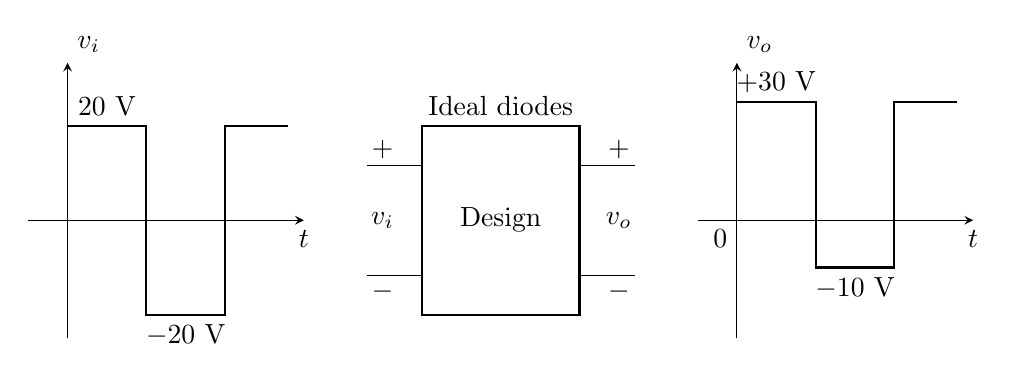
\begin{tikzpicture}[scale=1.0, >=stealth]
        
        % ==========================================
        % LEFT GRAPH: Input Waveform (v_i)
        % ==========================================
        % Axes
        \draw[->] (-0.5, 0) -- (3, 0) node[below] {$t$};
        \draw[->] (0, -1.5) -- (0, 2) node[above right] {$v_i$};
        
        % Waveform (+20V to -20V)
        \draw[thick] (0, 1.2) -- (1, 1.2) -- (1, -1.2) -- (2, -1.2) -- (2, 1.2) -- (2.8, 1.2);
        
        % Waveform Labels
        \node[above] at (0.5, 1.2) {$20\text{ V}$};
        \node[below] at (1.5, -1.2) {$-20\text{ V}$};
        
        % ==========================================
        % MIDDLE DIAGRAM: Design Block
        % ==========================================
        % The Block Box
        \draw[thick] (4.5, -1.2) rectangle (6.5, 1.2);
        \node at (5.5, 0) {Design};
        \node[above] at (5.5, 1.2) {Ideal diodes};
        
        % Left Input Terminals
        \draw (3.8, 0.7) -- (4.5, 0.7);
        \draw (3.8, -0.7) -- (4.5, -0.7);
        \node at (4.0, 0.9) {$+$};
        \node at (4.0, -0.9) {$-$};
        \node at (4.0, 0) {$v_i$};
        
        % Right Output Terminals
        \draw (6.5, 0.7) -- (7.2, 0.7);
        \draw (6.5, -0.7) -- (7.2, -0.7);
        \node at (7.0, 0.9) {$+$};
        \node at (7.0, -0.9) {$-$};
        \node at (7.0, 0) {$v_o$};
        
        % ==========================================
        % RIGHT GRAPH: Output Waveform (v_o)
        % ==========================================
        % Axes
        \draw[->] (8, 0) -- (11.5, 0) node[below] {$t$};
        \draw[->] (8.5, -1.5) -- (8.5, 2) node[above right] {$v_o$};
        \node[below left] at (8.5, 0) {$0$};
        
        % Waveform (+30V to -10V)
        \draw[thick] (8.5, 1.5) -- (9.5, 1.5) -- (9.5, -0.6) -- (10.5, -0.6) -- (10.5, 1.5) -- (11.3, 1.5);
        
        % Waveform Labels
        \node[above] at (9, 1.5) {$+30\text{ V}$};
        \node[below] at (10, -0.6) {$-10\text{ V}$};
        
        
    \end{tikzpicture}
\end{center}
\mk{12} \yr{EEE 263 | L-2/T-1 | 2022--23}


\item For the following circuit, draw the output waveshape for the given square input waveshape.
\begin{center}
    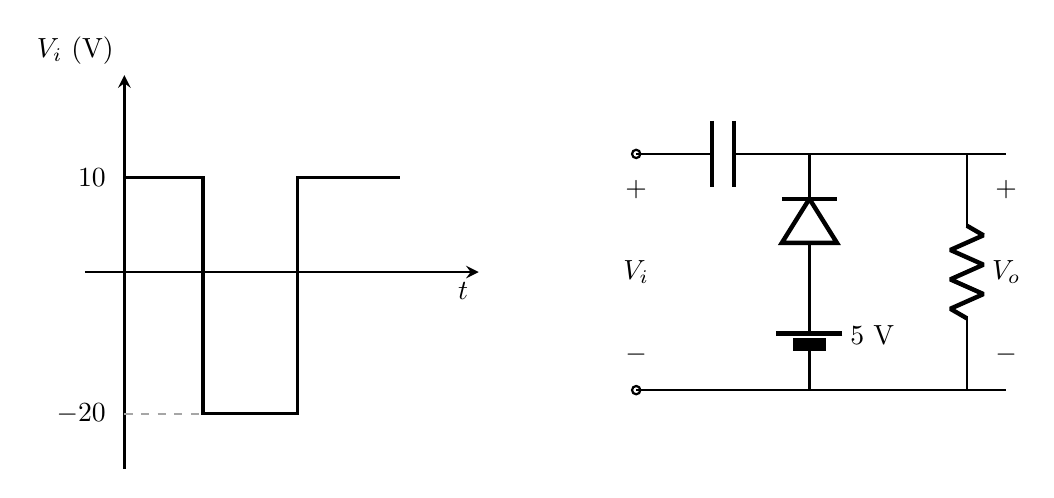
\begin{tikzpicture}[american, line width=0.8pt]

    % =========================================================================
    % LEFT SIDE: Input Waveform Graph (Vi vs t)
    % =========================================================================
    \begin{scope}[shift={(0,0)}]
        % Axes
        \draw[->, >=stealth, line width=1pt] (-0.5, 0) -- (4.5, 0) node[below left] {$t$};
        \draw[->, >=stealth, line width=1pt] (0, -2.5) -- (0, 2.5) node[above left] {$V_i\text{ (V)}$};

        % Square Waveform Path
        \draw[line width=1.2pt, color=black] 
            (0, 1.2) -- (1.0, 1.2) -- (1.0, -1.8) -- (2.2, -1.8) -- (2.2, 1.2) -- (3.5, 1.2);

        % Dashed helper line for negative peak
        \draw[dashed, color=gray!70] (0, -1.8) -- (1.0, -1.8);

        % Y-Axis Labels
        \node[left=3pt] at (0, 1.2) {$10$};
        \node[left=3pt] at (0, -1.8) {$-20$};
    \end{scope}


    % =========================================================================
    % RIGHT SIDE: Clamping Circuit Diagram
    % =========================================================================
    % Shifted to x=6.5 to give plenty of free drawing space and avoid overlap
    \begin{scope}[shift={(6.5,0)}]
        
        % Input Terminals
        \coordinate (in_top) at (0, 1.5);
        \coordinate (in_bot) at (0, -1.5);
        
        \draw (in_top) circle (1.5pt);
        \draw (in_bot) circle (1.5pt);
        
        % Input Voltage Label (+ Vi -)
        \draw (in_top) to[open, v=$V_i$] (in_bot);

        % Top wire through Capacitor
        \draw (in_top) to[C, name=C1] (2.2, 1.5) coordinate (junction_top);
        
        % Diode and DC Voltage Source Branch (Middle)
        % Diode points upwards, 5V Battery oriented with positive terminal up
        \draw (junction_top) to[diode, invert] (2.2, -0.2)
                            to[battery2, l=$5\text{ V}$] (2.2, -1.5) coordinate (junction_bot);

        % Parallel Resistor and Output Terminal Branch (Right)
        \draw (junction_top) -- (4.2, 1.5) coordinate (out_top)
              to[R, name=R1] (4.2, -1.5) coordinate (out_bot)
              -- (junction_bot);

        % Bottom Return Wire to Input
        \draw (junction_bot) -- (in_bot);

        % Output Voltage Label (+ Vo -)
        \draw (out_top) -- ++(0.5,0) coordinate (ext_top);
        \draw (out_bot) -- ++(0.5,0) coordinate (ext_bot);
        \draw (ext_top) to[open, v=$V_o$] (ext_bot);

    \end{scope}

    % =========================================================================
    % GLOBAL CAPTION
    % =========================================================================
\end{tikzpicture}
\end{center}
\mk{16} \yr{EEE 263 | L-2/T-1 | Jan 2021}


\item For the circuit shown, neatly draw the output waveform ($v_o$) corresponding to the input waveform ($v_{in}$) in steady state. Assume the diode is non-ideal.
\begin{center}
  
    \begin{circuitikz}[thick,scale=1.1, transform shape]
        
        % ==========================================
        % বাম দিকের অংশ: Input Graph (Square Wave)
        % ==========================================
        \begin{scope}[shift={(0,0)}]
            % Axes (অক্ষ)
            \draw[->, thick] (0,-1.8) -- (0,1.8) node[above] {$v_{in}$};
            \draw[->, thick] (0,0) -- (3.5,0) node[right] {$t$};
            
            % Square Wave (স্কয়ার ওয়েভ)
            \draw[thick] (0,1.2) -- (0.8,1.2) -- (0.8,-1.2) -- (1.6,-1.2) -- (1.6,1.2) -- (2.4,1.2) -- (2.4,-1.2) -- (3.2,-1.2);
            
            % Y-axis labels (ভোল্টেজ লেবেল)
            \node[left] at (0,1.2) {$+5\mathrm{V}$};
            \node[left] at (0,-1.2) {$-5\mathrm{V}$};
            
            % Dotted lines and Time label (সময় লেবেল)
            \draw[dashed] (0,-1.2) -- (0.8,-1.2);
            \draw[dashed] (1.6,0) -- (1.6,-1.5);
            \node[below] at (1.6, -1.5) {$1\mathrm{ms}$};
        \end{scope}
        
        % ==========================================
        % ডান দিকের অংশ: Diode Circuit
        % ==========================================
        \begin{scope}[shift={(5,-1)}]
            % 1. Square Wave Voltage Source
            \draw (0,0) to[sqV] (0,2.4);
            \node[left] at (-0.4, 2.4) {$+$};
            \node[left] at (-0.6, 1.2) {$v_{in}$};
            \node[left] at (-0.4, 0) {$-$};
            
            % 2. Top Branch (Series Resistor & Capacitor)
            \draw (0,2.4) to[R, l={$1\mathrm{K}$}] (2,2.4) to[C, l={$10\mu\mathrm{F}$}] (4.5,2.4);
            
            % 3. Parallel Branches (Diode & Resistor)
            \draw (4.5,0) to[empty diode] (4.5,2.4); % Diode pointing upwards
            \draw (6.5,0) to[R, l={$2\mathrm{K}$}] (6.5,2.4); % Parallel Resistor
            
            % 4. Connections & Bottom Wire
            \draw (4.5,2.4) -- (6.5,2.4);
            \draw (0,0) -- (6.5,0);
            
            % 5. Junction Dots
            \fill (4.5,2.4) circle (1.5pt);
            \fill (4.5,0) circle (1.5pt);
            \fill (6.5,2.4) circle (1.5pt);
            \fill (6.5,0) circle (1.5pt);
            
            % 6. Output Terminals
            \draw (6.5,2.4) to[short, -o] (8,2.4);
            \draw (6.5,0) to[short, -o] (8,0);
            
            \node[right] at (8.1, 2.4) {$+$};
            \node[right] at (8.1, 1.2) {$v_o$};
            \node[right] at (8.1, 0) {$-$};
            
        \end{scope}
        
    \end{circuitikz}
\end{center}
\mk{15} \yr{EEE 263 | L-2/T-1 | 2015--16}

\item Draw the output wave shape ($v_0$) and also the $V_L$--$V_o$ graph for the circuit shown. Assume a constant 0.7\,V forward voltage drop across the diode.
\begin{center}
  
    \begin{circuitikz}[thick,scale=1.2, transform shape]

        % ===================================================
        % Left Side: AC Voltage Source
        % ===================================================
        % Notice the extra { } around the label to prevent the "=" sign error
        \draw (0,0) to[sinusoidal voltage source, l={$v_i = 3\sin(\omega t)$}] (0, 2.5);

        % ===================================================
        % Top Side: Curved Capacitor
        % ===================================================
        \draw (0, 2.5) -- (0.5, 2.5) coordinate (c_left);
        \draw (c_left) to[cC] (2.5, 2.5) coordinate (c_right);
        \draw (c_right) -- (3, 2.5);

        % ===================================================
        % Output Terminals (v0)
        % ===================================================
        \draw (c_left) -- ++(0, 0.5) node[draw, fill=white, minimum size=3.5pt, inner sep=0pt] {};
        \draw (c_right) -- ++(0, 0.5) node[draw, fill=white, minimum size=3.5pt, inner sep=0pt] {};
        
        \node[above] at (1.5, 2.9) {$+ \quad v_0 \quad -$};

        % ===================================================
        % Right Side: Diode and Battery (1v)
        % ===================================================
        \draw (3, 2.5) to[D] (3, 1.25);
        \draw (3, 1.25) to[battery1, l={$1\text{v}$}] (3, 0);

        % ===================================================
        % Bottom Side: Return Wire
        % ===================================================
        \draw (3, 0) -- (0, 0);

    \end{circuitikz}
\end{center}


\mk{20} \yr{EEE 263 | L-2/T-1 | 2013--14}

\item Design a clamper circuit to perform the function indicated in the figure using an ideal diode.

\begin{center}
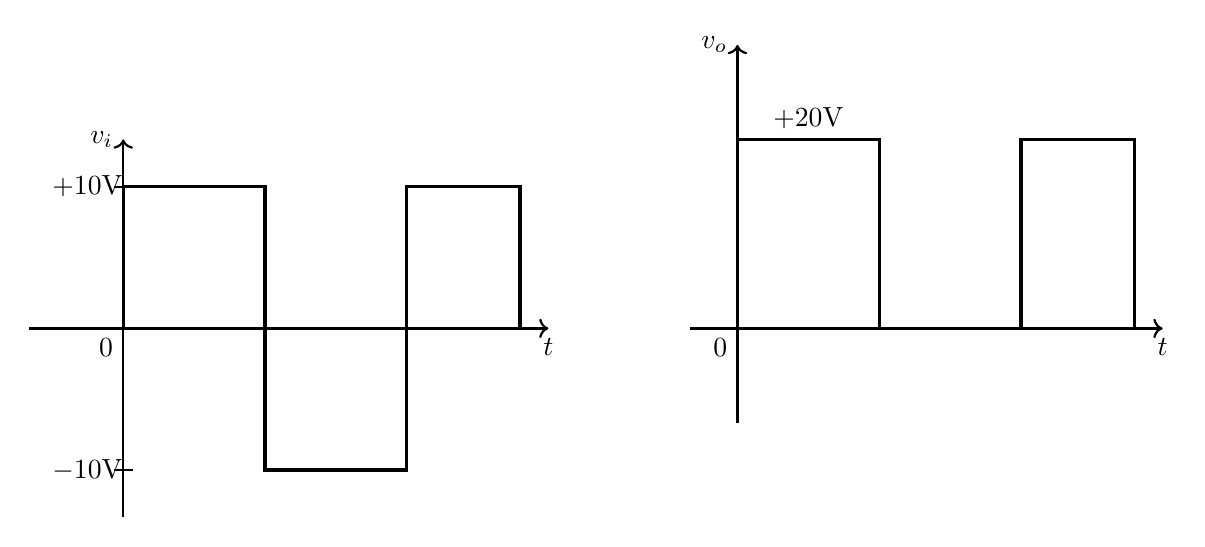
\begin{tikzpicture}[thick,scale=1.2]

  % ==========================================
  % বাম দিকের গ্রাফ: ইনপুট ভোল্টেজ (v_i)
  % ==========================================
  \begin{scope}[xshift=0cm]
    % X এবং Y অক্ষ (Axes)
    \draw[->, thick] (-1, 0) -- (4.5, 0) node[below] {$t$};
    \draw[->, thick] (0, -2) -- (0, 2) node[left] {$v_i$};
    
    % লেবেল এবং টিক মার্ক (Labels & Ticks)
    \node[below left] at (0,0) {0};
    \draw[thick] (-0.1, 1.5) -- (0.1, 1.5) node[left] {$+10\text{V}$};
    \draw[thick] (-0.1, -1.5) -- (0.1, -1.5) node[left] {$-10\text{V}$};
    
    % স্কয়ার ওয়েভ (Square Waveform)
    \draw[very thick] (0,0) -- (0,1.5) -- (1.5,1.5) -- (1.5,-1.5) -- (3,-1.5) -- (3,1.5) -- (4.2,1.5) -- (4.2,0);
  \end{scope}

  % ==========================================
  % ডান দিকের গ্রাফ: আউটপুট ভোল্টেজ (v_o) (Clamped Wave)
  % ==========================================
  \begin{scope}[xshift=6.5cm]
    % X এবং Y অক্ষ (Axes)
    \draw[->, thick] (-0.5, 0) -- (4.5, 0) node[below] {$t$};
    \draw[->, thick] (0, -1) -- (0, 3) node[left] {$v_o$};
    
    % লেবেল (Labels)
    \node[below left] at (0,0) {0};
    % +20V লেবেলটি প্রথম ওয়েভের উপরে বসানো হয়েছে ছবির মতো
    \node[above] at (0.75, 2) {$+20\text{V}$}; 
    
    % স্কয়ার ওয়েভ (Square Waveform)
    \draw[very thick] (0,0) -- (0,2) -- (1.5,2) -- (1.5,0) -- (3,0) -- (3,2) -- (4.2,2) -- (4.2,0);
  \end{scope}

\end{tikzpicture}
\end{center}

\mk{12} \yr{EEE 263 | L-2/T-1 | 2011--12}



\end{enumerate}

%%──────────────────────────────────────────────────────────────────────
\subtopic{cB}{Switching Circuits --- Logic Gates using BJTs}
\label{sub:s4-switching}

\begin{enumerate}\item Make a NAND and a NOR gate using BJTs.
\mk{10} \yr{EEE 263 | L-2/T-1 | 2012--13}

\end{enumerate}

%%──────────────────────────────────────────────────────────────────────
\subtopic{cB}{BJT Inverter Analysis}
\label{sub:s4-inverter}

\begin{enumerate}\item 
  \begin{enumerate}\item Modify both the $V_o$--$V_{in}$ and $I_c$--$V_{in}$ graphs if supply voltage is decreased from 5\,V to 2.5\,V ($R_c \approx 480\,\Omega$).
\mk{10} \yr{EEE 263 | L-2/T-1 | 2013--14}

\begin{center}
      \begin{circuitikz}[thick,scale=1.2, transform shape]

        % ===================================================
        % NPN Transistor
        % ===================================================
        \node[npn] (Q) at (0,0) {};

        % ===================================================
        % Emitter Connection (Ground)
        % ===================================================
        \draw (Q.E) -- ++(0, -0.5) node[ground] {};

        % ===================================================
        % Collector Connection (Rc, 5V, Output V0)
        % ===================================================
        % Output Node V0
        \draw (Q.C) to[short, -o] ++(1, 0) node[below] {$V_0$};
        
        % Resistor Rc and +5V supply
        % FIX: Added {...} around the label so the '=' sign doesn't break the code
        \draw (Q.C) to[R, l_={$R_C=480\,\Omega$}] ++(0, 2) coordinate (VCC);
        
        % Upward arrow for 5V supply
        \draw[->, >=stealth] (VCC) -- ++(0, 0.6) node[right] {$5\text{V}$};

        % ===================================================
        % Base Connection (Vin and Ground)
        % ===================================================
        % Wire from base to the left
        \draw (Q.B) -- ++(-1.5, 0) coordinate (VB);
        
        % DC Voltage source (battery) and ground
        % FIX: Added {...} around the label here as well for safety
        \draw (VB) to[battery1, l={$V_{\text{in}}$}] ++(0, -1.5) node[ground] {};

    \end{circuitikz}
        \begin{tikzpicture}[thick,scale=1.2]

        % ===================================================
        % Axes
        % ===================================================
        % Y-axis (V0)
        \draw[->, thick] (0, -0.5) -- (0, 5.5) node[left] {$V_0$};
        % X-axis (Vin)
        \draw[->, thick] (-0.5, 0) -- (6.5, 0) node[below] {$V_{\text{in}}$};

        % ===================================================
        % Piecewise Linear Curve
        % ===================================================
        % The path goes from x=0 -> x=2.5 -> x=4 -> x=5.5
        \draw[very thick] (0, 4) 
            -- (2.5, 4) coordinate (P1) 
            -- (4, 0.5) coordinate (P2) 
            -- (5.5, 0.5);

        % ===================================================
        % Highlight Circles at the corner points
        % ===================================================
        \draw[thick] (P1) circle (4pt);
        \draw[thick] (P2) circle (4pt);

        % ===================================================
        % Text Labels for the points
        % ===================================================
        \node[above right, xshift=2pt] at (P1) {$(0.5\text{v}, 5\text{v})$};
        \node[above right, xshift=2pt] at (P2) {$(0.7\text{v}, 0.2\text{v})$};

    \end{tikzpicture}
\end{center}


\item The figure shows an inverter gate built by an npn BJT and its $V_o$--$V_{in}$ characteristics. Copy the $V_o$--$V_{in}$ graph to your answer script exactly to scale and then draw the collector current ($I_c$) vs.\ $V_{in}$ over the same graph. Mention the co-ordinates of the bending points of the $I_c$--$V_{in}$ graph as shown for $V_o$--$V_{in}$.

\mk{16} \yr{EEE 263 | L-2/T-1 | 2012--13}

\item Modify both the $V_o$--$V_{in}$ and $I_c$--$V_{in}$ graphs if $R_c$ is infinity.
\mk{10} \yr{EEE 263 | L-2/T-1 | 2012--13}

\item Modify both the $V_o$--$V_{in}$ and $I_c$--$V_{in}$ graphs if supply voltage is increased from 5\,V to 10\,V ($R_c=480\,\Omega$).
\mk{10} \yr{EEE 263 | L-2/T-1 | 2012--13}

\item If the BJT in active mode shows a linear $I_c$--$V_{BE}$ behaviour instead of exponential, does voltage gain change with change in bias voltage $V_{in}$? Does output voltage swing change with the change in $V_{in}$? Explain why.
\mk{5} \yr{EEE 263 | L-2/T-1 | 2012--13}

\end{enumerate}

\end{enumerate}

%%──────────────────────────────────────────────────────────────────────
\subtopic{cB}{CMOS Inverter Analysis}
\label{sub:s4-cmos}

\begin{enumerate}\item The inverter circuit with CMOS shown has $k_n'(W_n/L_n) = k_p'(W_p/L_p) = 1\,\text{mA/V}^2$ and $V_{tn}' = -V_{tp}' = 1\,\text{V}$. Find (i) $i_{DN}$, (ii) $i_{DP}$, (iii) $V_o$ for $V_{in} = -2.5\,\text{V}$.
\begin{center}
   \begin{circuitikz}[thick,scale=1.2, transform shape]
                              \ctikzset{tripoles/mos style/arrows}

        % ১. PMOS (Top) and NMOS (Bottom)
        \draw (0, 1.5) node[pmos] (Qp) {};
        \draw (0, -1.5) node[nmos] (Qn) {};
        
        % Transistor Labels
        \node[right] at (0.5, 1.5) {$Q_p$};
        \node[right] at (0.5, -1.5) {$Q_n$};
        
        % ২. Input (Gate connections)
        \draw (Qp.G) -- (Qn.G) coordinate[midway] (G_mid);
        \draw (G_mid) to[short, -o] (-1.5, 0) node[left] {$v_{in}$};
        
        % ৩. Output (Drain connections)
        \draw (Qp.D) -- (Qn.D) coordinate[midway] (D_mid);
        \draw (D_mid) -- (2, 0) coordinate (V_out) to[short, -o] (3, 0) node[right] {$v_o$};
        
        % Junction dot at output branch
        \fill (V_out) circle (1.5pt);
        
        % ৪. Power Supplies (Source connections)
        \draw (Qp.S) -- ++(0, 0.5) node[vcc] {$+2.5\mathrm{V}$};
        \draw (Qn.S) -- ++(0, -0.5) node[vee] {$-2.5\mathrm{V}$};
        
        % ৫. Load Resistor
        \draw (V_out) to[R, l={$10\mathrm{K}\Omega$}] (2, -2) node[ground] {};
        
        % ৬. Current Labels (Arrows pointing downwards)
        \draw[->, thick] (0.4, 0.8) -- (0.4, 0.2) node[midway, right] {$i_{Dp}$};
        \draw[->, thick] (0.4, -0.2) -- (0.4, -0.8) node[midway, right] {$i_{Dn}$};
        
    \end{circuitikz}
\end{center}
\mk{15} \yr{EEE 263 | L-2/T-1 | 2015--16}

\item For the CMOS inverter, draw $V_o$ for the given input $V_{in}$ waveform.

\begin{center}
          \begin{circuitikz}[thick,scale=1.2, transform shape]
                      \ctikzset{tripoles/mos style/arrows}

            % Place PMOS (Top) and NMOS (Bottom)
            % Drains are pointing towards each other
            \node[pmos, anchor=D] (P) at (0, 1.5) {};
            \node[nmos, anchor=D] (N) at (0, -0.5) {};
            
            % Connect Gates together and add Input Terminal (vin)
            \draw (P.G) -- (N.G) coordinate[midway] (G_mid);
            \draw (G_mid) to[short, *-o] ++(-1, 0) node[left] {$v_{in}$};
            
            % Connect Drains together and add Output Terminal (v0)
            \draw (P.D) -- (N.D) coordinate[midway] (D_mid);
            \draw (D_mid) to[short, *-o] ++(1, 0) node[right] {$v_0$};
            % VDD (5V) Connection at PMOS Source
            \draw[->, >=stealth] (P.S) -- ++(0, 0.6) node[right] {$5\text{V}$};
            
            % Ground (0V) Connection at NMOS Source
            \draw (N.S) -- ++(0, -0.6) node[ground] {} node[right=0.2cm] {$0$};


            
        \end{circuitikz}

    % ===================================================
    % 2nd Diagram: Square Waveform Graph (vin vs t)
    % ===================================================
  
        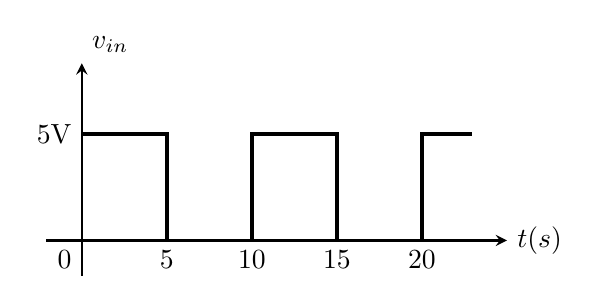
\begin{tikzpicture}[thick,scale=0.9]
            
            % X and Y Axes
            \draw[->, >=stealth] (-0.5, 0) -- (6, 0) node[right] {$t(s)$};
            \draw[->, >=stealth] (0, -0.5) -- (0, 2.5) node[above right] {$v_{in}$};
            
            % Y-axis Labels
            \node[left] at (0, 1.5) {$5\text{V}$};
            \node[below left] at (0, 0) {$0$};
            
            % X-axis Ticks/Labels
            \node[below] at (1.2, 0) {$5$};
            \node[below] at (2.4, 0) {$10$};
            \node[below] at (3.6, 0) {$15$};
            \node[below] at (4.8, 0) {$20$};
            
            % Draw the Square Wave Line
            \draw[very thick] (0, 1.5) 
                -- (1.2, 1.5) -- (1.2, 0) 
                -- (2.4, 0) -- (2.4, 1.5) 
                -- (3.6, 1.5) -- (3.6, 0) 
                -- (4.8, 0) -- (4.8, 1.5) 
                -- (5.5, 1.5);
                
        \end{tikzpicture}
\end{center}

\mk{15} \yr{EEE 263 | L-2/T-1 | 2013--14}

\end{enumerate}

%%──────────────────────────────────────────────────────────────────────
\subtopic{cB}{Digital vs.\ Analog Systems}
\label{sub:s4-digital}

\begin{enumerate}\item Why is digital processing of data advantageous over analog processing?
\mk{6} \yr{EEE 263 | L-2/T-1 | 2013--14}

\item Why do we need to miniaturize a transistor as much as possible? If you continue to miniaturize the transistor (switch), what problems may surface?
\mk{5} \yr{EEE 263 | L-2/T-1 | 2013--14}

\item Write a script in C language that takes a sinusoidal input and provides a full-wave rectified output.
\mk{5} \yr{EEE 263 | L-2/T-1 | 2013--14}

\item How does a computer program rectify the sinusoidal input mentioned above? Is there any diode inside the processor? If not, what makes that act of rectification possible?
\mk{10} \yr{EEE 263 | L-2/T-1 | 2013--14}

\end{enumerate}


%% ══════════════════════════════════════════════════════════════════════
%%  PART III
%% ══════════════════════════════════════════════════════════════════════
\secdivider{Part III --- Amplifiers}{BJT and MOSFET amplifier configurations, small-signal analysis, gain derivation}{cC}

%% ══════════════════════════════════════════════════════════════════════
%%  SECTION 5: BJT AMPLIFIERS
%% ══════════════════════════════════════════════════════════════════════
\markboth{S5: BJT Amplifiers}{S5: BJT Amplifiers}
\label{sec:S5}
\titleformat{\section}{\large\bfseries\color{cC}}{}{0em}{}[\titlerule]
\section*{S5 \quad BJT Amplifiers}
\addcontentsline{toc}{section}{S5: BJT Amplifiers}

%%──────────────────────────────────────────────────────────────────────
\subtopic{cC}{Common Emitter / Trans-conductance Amplifier}
\label{sub:s5-ce}

\begin{enumerate}\item The transistor shown is biased with a constant current $I=1\,\text{mA}$ and has $\beta=100$ and $V_A=100\,\text{V}$. (i) Find the DC voltages at the Base, Emitter, and Collector terminals. (ii) Find the small-signal equivalent circuit parameters $r_o$, $r_\pi$, $g_m$ and draw the hybrid-$\pi$ model. (iii) If the Z terminal is connected to ground, X is connected to $v_{sig}$ through $R_{sig}=2\,\text{k}\Omega$, and Y is connected to $R_L=8\,\text{k}\Omega$, find the overall voltage gain $v_y/v_{sig}$.
\begin{center}
\begin{circuitikz}[american, line width=0.8pt]

    % --- Transistor ---
    \node[npn] (Q) at (0,0) {};
    
    % Handwritten-style terminal labels (B, C, E)
    \node at (-0.7, 0.4) {B};
    \node at (-0.4, 1.2) {C};
    \node at (0.5, -0.8) {E};

    % --- Base Input Circuit (Left) ---
    \draw (Q.B) -- (-2.5,0);
    \fill (-2.5,0) circle (2pt);
    
    % Input X and Capacitor
    \draw (-5.5,0) node[left] {X} to[short, o-] (-5,0) to[C, l=$\infty$] (-2.5,0);
    
    % Base Resistor to Ground
    \draw (-2.5,0) to[R, l=$10\text{ k}\Omega$] (-2.5,-3) node[ground] {};


    % --- Collector Circuit (Top) ---
    \draw (Q.C) -- (0, 1.5);
    \fill (0, 1.5) circle (2pt);
    
    % Collector Resistor and VCC
    \draw (0, 1.5) to[R, l_=$8\text{ k}\Omega$] (0, 4);
    \draw[-latex, line width=1pt] (0, 4) -- (0, 5.2) node[above] {\textbf{+10 V}};


    % --- Emitter Circuit (Bottom) ---
    \draw (Q.E) -- (0, -1.5);
    \fill (0, -1.5) circle (2pt);
    
    % Tail Current Source
    \draw (0, -1.5) to[isource, l={$I = 1\text{ mA}$}] (0, -4);
    \draw[-latex] (0, -4) -- (0, -5.2);


    % --- Output Y (Top Right) ---
    \draw (0, 1.5) to[C, l=$\infty$] (3.5, 1.5) to[short, -o] (4.5, 1.5) node[right] {Y};


    % --- Output Z (Bottom Right) ---
    \draw (0, -1.5) to[C, l=$\infty$] (3.5, -1.5) to[short, -o] (4.5, -1.5) node[right] {Z};

\end{circuitikz}
\end{center}
\mk{20} \yr{EEE 263 | L-2/T-1 | 2024--25}

\item Determine the voltage gain $v_0/v_i$ of the transistor amplifier shown in the figure. Assume $\beta=100$.
\begin{center}
      \begin{circuitikz}[thick,scale=1.2, transform shape]
        
        % ==========================================
        % Transistor (PNP)
        % ==========================================
        % xscale=-1 flips the transistor so the base is on the right
        % For a PNP, Emitter (Q.E) is on top, Collector (Q.C) is on the bottom
        \draw (0,0) node[pnp, xscale=-1] (Q) {};
        
        % Base connection to Ground
        \draw (Q.B) -- (1, 0) node[ground] {};
        
        % ==========================================
        % Emitter Branch (Top)
        % ==========================================
        % Emitter node
        \draw (Q.E) -- (0, 1.5) coordinate (E_node);
        \node[circ] at (E_node) {};
        
        % Resistor RE and Positive Supply V+
        \draw (E_node) to[R, l_={$R_E = 10\text{ k}\Omega$}] (0, 3.5);
        \draw[-latex] (0, 3.5) -- (0, 4.2) node[above] {$V^+ = +10\text{ V}$};
        
        % Input Section (Left of Emitter)
        % Drawing leftwards: l places the label below the component
        \draw (E_node) to[C, l=$C_E$] (-2.2, 1.5) node[ocirc] {} 
              to[V, l_=$v_i$] (-2.2, -0.5) node[ground] {};
              
        % ==========================================
        % Collector Branch (Bottom)
        % ==========================================
        % Collector node
        \draw (Q.C) -- (0, -1.5) coordinate (C_node);
        \node[circ] at (C_node) {};
        
        % Resistor RC and Negative Supply V-
        % Drawing downwards: l places the label on the right side
        \draw (C_node) to[R, l=$R_C$, a=$5\text{ k}\Omega$] (0, -3.5);
        \draw[-latex] (0, -3.5) -- (0, -4.2) node[below] {$V^- = -10\text{ V}$};
        
        % Output Section (Right of Collector)
        % Drawing rightwards: l_ places the label below the component
        \draw (C_node) to[C, l_=$C_C$] (2.2, -1.5) node[ocirc] {} node[right] {$v_o$};
        
        % ==========================================
        % Caption
        % ==========================================
        
    \end{circuitikz}

\end{center}
\mk{26} \yr{EEE 263 | L-2/T-1 | 2017--18}

\item A CE amplifier utilizes a BJT with $\beta=100$ and $V_A=100\,\text{V}$, is biased at $I_C=1\,\text{mA}$ and has a collector resistance $R_C=5\,\text{k}\Omega$. Find $R_{in}$, $R_o$, and $A_{vo}$. If the amplifier is fed with a signal source having a resistance of 5\,k$\Omega$ and a load resistance $R_L=5\,\text{k}\Omega$ is connected to the output terminal, find the resulting $A_v$ and $G_v$. If $v_\pi$ is to be limited to 5\,mV, what are the corresponding $v_{sig}$ and $v_o$ with the load connected?
\mk{20} \yr{EEE 263 | L-2/T-1 | 2017--18}

\item For the circuit shown, determine small-signal parameters $g_m$, $r_\pi$, and $r_e$ for both transistors, the overall small-signal voltage gain $A_v = v_0/v_s$, input resistance $R_{in}$, and output resistance $R_{out}$. Here $\beta=120$.
\begin{center}
  
    % Scaled slightly to fit page widths, but internal coordinates are expanded
    \begin{circuitikz}[thick,x=1.3cm, transform shape]
        \ctikzset{resistors/scale=0.9, capacitors/scale=0.9}

        % ==========================================
        % Ground Rail (widened to 16 units)
        % ==========================================
        \draw (0,0) -- (16,0);
        \node[ground] at (8, 0) {};

        % ==========================================
        % Input Stage (Vs and C1)
        % ==========================================
        % Expanded Y-height to 4 for the midline, giving resistors more vertical space
        \draw (0,0) to[sV, l=$V_s$] (0, 4) to[C, l=$C_1$] (3, 4);
        
        % Rin arrow (Input Resistance) - positioned clearly below C1
        \draw[-latex] (1.2, 3.2) -- (2.2, 3.2) node[midway, below] {$R_{in}$};

        % ==========================================
        % Stage 1: Q1 Bias (R1, R2)
        % ==========================================
        % Top rail shifted up to Y=8 for extra label clearance
        \draw (3, 4) to[R, l={$R_1=67.3\text{ k}\Omega$}, *-] (3, 8);
        \draw (3, 4) to[R, l=$R_2$, a=$12.7\text{ k}\Omega$, *-*] (3, 0);

        % ==========================================
        % Stage 1: Q1 (Common Emitter)
        % ==========================================
        \node[npn] (Q1) at (5, 4) {};
        \node[right] at (Q1.text) {$Q_1$};
        \draw (3, 4) -- (Q1.B);

        % Q1 Collector Branch (Rc)
        \draw (Q1.C) to[R, l=$R_C$, a=$10\text{ k}\Omega$, *-*] (Q1.C |- 0, 8);
        
        % Q1 Emitter Branch (RE || CE)
        \draw (Q1.E) -- ++(0, -0.6) coordinate (E1);
        \draw (E1) -- ++(-1, 0) coordinate (E1L);
        \draw (E1) -- ++(1, 0) coordinate (E1R);
        \node[circ] at (E1) {};
        
        % Generous spacing for Emitter components
        \draw (E1L) to[R, l_=$R_E$, a^=$2\text{ k}\Omega$] (E1L |- 0, 0);
        \draw (E1R) to[C, l=$C_E$] (E1R |- 0, 0);
        \node[circ] at (E1L |- 0, 0) {};
        \node[circ] at (E1R |- 0, 0) {};

        % ==========================================
        % Inter-stage Coupling C2
        % ==========================================
        % Widened horizontal run for C2 to avoid Q1 and Q2 overlapping
        \draw (Q1.C) to[short, *-] ++(0.5, 0) to[C, l=$C_2$] ++(3, 0) coordinate (C2_out);
        \draw (C2_out) -| (10, 4);

        % ==========================================
        % Stage 2: Q2 Bias (R3, R4)
        % ==========================================
        \node[circ] at (10, 4) {};
        \draw (10, 4) to[R, l=$R_3$, a=$15\text{ k}\Omega$, *-*] (10, 8);
        \draw (10, 4) to[R, l=$R_4$, a=$45\text{ k}\Omega$, *-*] (10, 0);

        % ==========================================
        % Stage 2: Q2 (Emitter Follower)
        % ==========================================
        \node[npn] (Q2) at (12, 4) {};
        \node[right] at (Q2.text) {$Q_2$};
        \draw (10, 4) -- (Q2.B);

        % Q2 Collector Branch (Direct to Vcc)
        \draw (Q2.C) -- (Q2.C |- 0, 8);
        \node[circ] at (Q2.C |- 0, 8) {};

        % Q2 Emitter Branch (RE2)
        \draw (Q2.E) to[R, l=$R_{E2}$, a=$1.6\text{ k}\Omega$, *-*] (Q2.E |- 0, 0);

        % ==========================================
        % Output Section (C3, RL, and Vo)
        % ==========================================
        \draw (Q2.E) to[short, *-] ++(1, 0) coordinate (C3_in);
        \draw (C3_in) to[C, l=$C_3$] ++(2, 0) coordinate (Vout);
        \draw (Vout) to[R, l=$R_L$, a=$250\Omega$, *-*] (Vout |- 0, 0);
        
        % Output terminal with Vo perfectly spaced
        \draw (Vout) to[short, -o] ++(1, 0) node[right] {\large $V_o$};

        % Rout arrow (Output Resistance) - placed cleanly under C3
        \draw[-latex] (14.5, 2.5) -- (13.5, 2.5) node[midway, below] {$R_{out}$};

        % ==========================================
        % Top Vcc Rail
        % ==========================================
        \draw (3, 8) -- (12, 8);

    \end{circuitikz}
\end{center}
\mk{36} \yr{EEE 263 | L-2/T-1 | 2016--17}

\item For the circuit shown, determine $R_{in}$, $R_{out}$, $V_o/V_i$, and $i_o/i_i$. The BJT is biased with $I=5\,\text{mA}$ and has $\beta=100$ and $V_A=100\,\text{V}$.

\begin{center}
 
  \begin{circuitikz}[thick,scale=1.2, transform shape]
        
        % ===================================================
        % Emitter Follower (Common Collector) Amplifier
        % ===================================================
        
        % ১. Transistor (NPN)
        \node[npn] (Q) at (0, 0) {};
        
        % ২. Collector & Vcc Path
        \draw (Q.C) -- ++(0, 0.5) coordinate (Vcc);
        \draw[->, >=stealth] (Vcc) -- ++(0, 0.5) node[right] {$V_{CC}$};
        
        % ৩. Emitter Current Source & -Vee Path
        \draw (Q.E) -- ++(0, -0.5) coordinate (E_node);
        \draw (E_node) to[I, l={$I=5\mathrm{mA}$}] ++(0, -1.8) coordinate (Vee);
        \draw[->, >=stealth] (Vee) -- ++(0, -0.5) node[right] {$-V_{EE}$};
        
        % ৪. Input Side (Left)
        \draw (Q.B) ++(-2, 0) coordinate (vi_node) to[C, l=$\infty$] (Q.B);
        \node[ocirc] at (vi_node) {};
        \node[below] at (vi_node) {$+v_i$};
        
        \draw (vi_node) ++(-2.5, 0) coordinate (Vs_top);
        \draw (Vs_top) to[R, l_={$R_s=10\mathrm{K}\Omega$}, i^>={$i_i$}] (vi_node);
        \draw (Vs_top) to[V, l_=$V_s$] ++(0, -2.5) node[ground]{};
        
        % Rin Arrow
        \draw[->, >=stealth] ([shift={(-0.4, -0.8)}]vi_node) node[below] {$R_{in}$} -- ++(0.8, 0);
        
        % ৫. Output Side (Right)
        \draw (Q.E) to[short, *-] ++(0.5, 0) coordinate (E_branch);
        \draw (E_branch) to[C, l=$\infty$] ++(2, 0) coordinate (vo_node);
        \node[circ] at (vo_node) {}; % এখানে জাংশন বোঝাতে circ (ডট) দেওয়া হয়েছে
        
        % Load Resistor RL
        \draw (vo_node) to[R, l={$R_L=1\mathrm{K}\Omega$}, i^>={$i_o$}] ++(0, -2.5) node[ground]{};
        
        % vo terminal and Output current io
        % ওভারল্যাপ এড়াতে i_o কে ডানদিকের লাইনে আরেকটু সরিয়ে (i^> ব্যবহার করে) দেওয়া হয়েছে
        \draw (vo_node) -- ++(0.5, 0) coordinate (io_start);
        \draw (io_start) to[short] ++(1.5, 0) node[ocirc]{} node[right] {$V_o$};
        
        % Rout Arrow
        % Rout অ্যারোটিকে RL এর বাঁ-পাশে সরিয়ে দেওয়া হয়েছে যেন কোনো ওভারল্যাপ না হয়
        \draw[->, >=stealth] ([shift={(-0.57, -0.6)}]vo_node) node[below] {$R_{out}$} -- ++(-0.8, 0);
        
    \end{circuitikz}
\end{center}

\mk{20} \yr{EEE 263 | L-2/T-1 | 2014--15}

\item Draw the small signal circuit diagram of the CE circuit shown. Why is the circuit called a ``Small Signal'' circuit? Determine the values of input resistance $R_{in}$, output resistance $R_{out}$, and voltage gain $A_v$. If $v_{sig} \approx 2\,\text{mV}$, find the value of $V_{out}$.

\begin{center}
      \begin{circuitikz}[thick,scale=1.2, transform shape]
        
        % ===================================================
        % NPN Transistor (Center point of the circuit)
        % ===================================================
        \node[npn] (Q) at (0,0) {};
        
        % ===================================================
        % Base Circuit (Left side)
        % ===================================================
        \draw (Q.B) -- ++(-1,0) coordinate (B_node);
        
        % 100k ohm Resistor to ground
        \draw (B_node) to[R, l=$100\text{k}\Omega$] (B_node |- 0,-2.5) node[ground]{};
        
        % Input AC Source and Curved Capacitor
        \draw (B_node) ++(-2,0) coordinate (V_in_top);
        % cC draws a capacitor with the right side curved
        \draw (V_in_top) to[cC] (B_node); 
        \draw (V_in_top) to[sinusoidal voltage source, l=$V_{sig}$] (V_in_top |- 0,-2.5) node[ground]{};

        % ===================================================
        % Emitter Circuit (Bottom side)
        % ===================================================
        % DC Voltage source (10v). Drawing downwards puts '+' at the top
        \draw (Q.E) to[V, l={$10\text{v}$}] (Q.E |- 0,-2.5) node[ground]{};

        % ===================================================
        % Collector Circuit (Top side)
        % ===================================================
        % 8k ohm Resistor going up, then right, then grounded
        \draw (Q.C) to[R, l=$8\text{k}\Omega$] ++(0,2.5) coordinate (Rc_top);
        \draw (Rc_top) -- ++(1.5,0) -- ++(0,-0.5) node[ground]{};

        % ===================================================
        % Output Circuit (Right side)
        % ===================================================
        % Coupling Capacitor
        \draw (Q.C) to[cC] ++(2.5,0) coordinate (Out_node); 
        
        % 10k ohm Load Resistor
        \draw (Out_node) to[R, l=$10\text{k}\Omega$] (Out_node |- 0,-2.5) node[ground]{};
        
        % Output Terminal (Vout)
        \draw (Out_node) to[short, -o] ++(0.7,0) node[right]{$V_{out}$};

    \end{circuitikz}
\end{center}

\mk{36} \yr{EEE 263 | L-2/T-1 | 2013--14}

\item The figure shows the basic structure of a trans-conductance amplifier to be implemented by a BJT. Given $AV_{in}=I_c R_{out}$ along with $R_{sig}\approx 0$ and the load ($R_L$) can be much greater than $R_{out}$; which BJT configuration (common emitter, common base, or common collector) will you choose for best performance? Explain why. Comment on its gain and loading effect.

\begin{center}
  
\begin{circuitikz}[thick,american, thick]
    % Global thickening for better readability like in the sketch
    \ctikzset{thickness=1.5}

    % -- INPUT SIDE --
    % Start ground connection and draw AC voltage source to top rail
    \draw (0,0) coordinate (ground) 
          to[sV, l=$V_{\text{sig}}$] (0,2) coordinate (in_T);
          
    % Connection at ground level
    \draw (0,0) -- (3,0); % Extending to input of internal block
          
    % From top source connection, horizontal connection, then R_sig resistor
    % Extend wire a bit before adding component, then to main rectangle
    \draw (in_T) to[short] (1,2)
          to[R, l=$R_{\text{sig}}$] (3,2);

    % -- INTERNAL BLOCK BOUNDARIES AND COMPONENTS --
    % Define coordinates for the main central rectangle (block). 
    % Top rail at y=2, bottom rail at y=0. Width of 6 units.
  
    
    % Draw the rectangle boundary first, with regular line thickness
   
    
    % Node for figure caption centre bottom relative to figure extent. Figure centred.

    % Connection of outer circuit to inner block. 
    % Drawing short lines first helps avoid component crossing.

    % Internal R_in resistor, vertically placed with manual signs.
    % Drawing from top to bottom (standard), with pos relative text placement.
    \draw (3,2) to[R, l=$R_{\text{in}}$] (3,0);
    % Manual positioning of + and - signs, and V_in label.
    % Nodes placed on wire with small horizontal offsets.
    \draw[black] (2.6, 1.6) node {\footnotesize $+$}
                   (2.6, 0.4) node {\footnotesize $-$}
                   (2.6, 1) node {\footnotesize $V_{\text{in}}$};

    % Central parallel component: Dependent Current Source. 
    % Constructed with manual TikZ for this specific composed look (diamond with arrow).
    \coordinate (ds_top) at (6,2);
    \coordinate (ds_bot) at (6,0);
    % Create diamond node with label on left. Position label text with left offset.
    \node[diamond, draw, minimum size=1cm, fill=white] (dsource) at (6,1) {};
    \node[left=0.1cm] at (5.5, 1) {$A v_{\text{in}}$};
    % Draw connection lines to rails
    \draw (ds_top) -- (dsource.north);
    \draw (ds_bot) -- (dsource.south);
    % Draw standard style arrow inside diamond. Latex arrow head style.
    \draw[->, >=latex] (6, 0.6) -- (6, 1.4);

    % Output interface resistor R_out (parallel to dependent source) at, say, x=8.
    \draw (8,2) to[R, l=$R_{\text{out}}$] (8,0);

    % Inner rails connecting components. Ambiguity check.
    \draw (6,2) -- (9,2); % Top Rail internal

    % -- OUTPUT SIDE --
    % Start output from rectangle top-right corner, coordinate (9,2).
    % Use relative offset for clean placement. Short wire extension.
    \draw (9,2) -- ++(1,0) coordinate (extT_pre);
    % Define load resistor vertical placement. At, say, x=11.
    \coordinate (loadT) at (11,2);
    % Draw the output current arrow and label 'i_L' on the wire extension. 
    % Note on current label position: Standard 'i' option places label outside direction, 
    % image text seems standard placement for controlled direction relative to other labels. 
    % Let's use standard placement. Current flowing right.
    \draw (extT_pre) to[short, i=$i_{\text{L}}$] (loadT);
    % Component vertical
    \draw (loadT) to[R, l=$R_{\text{L}}$] (11,0);
    % Return wire complete connection back to internal ground rail start point (9,0).
    \draw (11,0) -- (6,0);
    
    % Global Ground rail - ensure explicit connection across entire bottom for clarity.

    % Overall figure label "Figure 2(a)". Centre below the total figure.
    % Left side x=0, total width 11. Total centre x=5.5.

\end{circuitikz}
\end{center}

\mk{20} \yr{EEE 263 | L-2/T-1 | 2012--13}

\item Consider the emitter degenerated CE circuit of Fig. for Q. No. 8(b).
    \begin{enumerate}
        \item[(i)] Find the DC current $I_C$ and DC voltage $V_C$, $V_B$ and $V_E$. Assume $\beta = 100$, $V_{BE} = 0.7\text{ V}$.
        \item[(ii)] What are the allowable signal swings at the collector in both directions?
        \item[(iii)] Determine the values of the BJT small signal model parameter: $r_\pi$, $r_e$, $g_m$ at this bias point.
        \item[(iv)] Draw the complete small signal equivalent circuit of the amplifier using suitable model of BJT. Neglect $r_0$.
        \item[(v)] Find the value of $R_e$ that results in $R_{\text{in}}$ equal to four times the source resistance $R_{\text{sig}}$.
        \item[(vi)] For this value of $R_e$, find $A_{vo}$, $R_{\text{out}}$, $A_v$, $G_v$ and $A_{is}$ of the amplifier.
    \end{enumerate}


\begin{center}
\begin{circuitikz}[thick,american, thick, scale=1.1, transform shape]

  % ==========================================
  % NPN Transistor
  % ==========================================
  \node[npn] (Q) at (0,0) {};

  % ==========================================
  % Collector Branch & Vcc
  % ==========================================
  \draw (0, 3.5) node[vcc] {$V_{CC} = +10\text{ V}$}
        to[R, l={ $R_C = 8\text{ k}\Omega$ }, i={ $I_C$ }] (0, 1)
        coordinate (Vc_node) 
        -- (Q.C);
        
  \draw[fill=black] (Vc_node) circle (1.5pt);
  \node[left] at (Vc_node) {$V_C$};

  % ==========================================
  % Base Branch & Input Section
  % ==========================================
  % বেস নোডটিকে একটু বামে সরানো হয়েছে যেন কোনো overlap না হয়
  \draw (Q.B) -- ++(-1.5,0) coordinate (Vb_node);
  \draw[fill=black] (Vb_node) circle (1.5pt);
  \node[above] at (Vb_node) {$V_B$};

  % Base resistor (R_B) - l_ ব্যবহার করে টেক্সট বামে আনা হয়েছে
  \draw (Vb_node) to[R, l_={ $R_B = 100\text{ k}\Omega$ }] ++(0,-2.5) node[ground]{};

  % Input signal (C1, R_sig, v_sig)
  \draw (Vb_node) to[C, l_={ $C_1$ }] ++(-2,0)
        to[R, l_={ $R_{\text{sig}} = 5\text{ k}\Omega$ }] ++(-2.5,0)
        to[V, l={ $v_{\text{sig}}$ }] ++(0,-2.5) node[ground]{};

  % R_in arrow
  \draw[-stealth] (-1.5, -4) node[below]{$R_{\text{in}}$} |- (-2.2, -0.9);

  % ==========================================
  % Base-Emitter Voltage (v_pi) - + এবং - চিহ্ন ঠিক করা হয়েছে
  % ==========================================
  \node[font=\footnotesize] at (-0.8, -0.15) {$+$};
  \node[font=\footnotesize] at (-0.8, -0.65) {$-$};
  \node[left] at (-0.9, -0.4) {$v_\pi$};

  % ==========================================
  % Emitter Branch (R_e, Current Source, C3)
  % ==========================================
  \draw (Q.E) -- ++(0,-0.5) coordinate (Ve_node);
  \draw[fill=black] (Ve_node) circle (1.5pt);
  \node[right] at (Ve_node) {$V_E$};

  % R_e
  \draw (Ve_node) to[R, l={ $R_e$ }] ++(0,-2) coordinate (I_node);
  \draw[fill=black] (I_node) circle (1.5pt); 

  % Current Source to -V_EE
  \draw (I_node) to[isource, l={ $I = 1\text{ mA}$ }] ++(0,-2)
        node[vee] {$-V_{EE} = -10\text{ V}$};

  % Emitter bypass capacitor (C3) connected from the middle node
  \draw (I_node) -- ++(3.5,0) to[C, l={ $C_3$ }] ++(0,-2) node[ground]{};

  % ==========================================
  % Output Branch (C2, R_L, v_o)
  % ==========================================
  \draw (Vc_node) to[C, l={ $C_2$ }] ++(3.5,0) coordinate (Vout_node);
  \draw[fill=black] (Vout_node) circle (1.5pt);
  
  \draw (Vout_node) to[short, -o] ++(1,0) node[right]{$v_o$};
  \draw (Vout_node) to[R, l={ $R_L = 5\text{ k}\Omega$ }] ++(0,-2.5) node[ground]{};

\end{circuitikz}
\end{center}


\mk{36} \yr{EEE 263 | L-2/T-1 | 2011--12}

\end{enumerate}

%%──────────────────────────────────────────────────────────────────────
\subtopic{cC}{Common Base Amplifier}
\label{sub:s5-cb}

\begin{enumerate}\item For a Common Base Amplifier, using the appropriate small-signal equivalent model, derive the expressions of input resistance, output resistance, open-circuit voltage gain, and overall voltage gain.
\mk{14} \yr{EEE 263 | L-2/T-1 | 2022--23}

\end{enumerate}

%%──────────────────────────────────────────────────────────────────────\n\subtopic{cC}{Bootstrapped Follower}
\label{sub:s5-bootstrap}

\begin{enumerate}

\item For the bootstrapped follower circuit shown: (i) Find the DC emitter current and $g_m$, $r_e$, $r_\pi$. Assume $\beta=100$. (ii) Replace the BJT with its T model (neglecting $r_o$) and determine $R_{in}$ and the voltage gain $v_o/v_{sig}$. (iii) Repeat (ii) for the case when capacitor $C_B$ is open-circuited. Compare the results with (ii) and comment on the advantage of bootstrapping.
\begin{center}
    
\begin{circuitikz}[american, line width=0.8pt, y=1.3cm, x=1.5cm]

    % --- Transistor ---
    \node[npn] (Q) at (6, 5.5) {};
    
    % --- Collector & +9V ---
    \draw (Q.C) -- (6, 7.0);
    \draw[-latex, line width=1pt] (6, 7.0) -- (6, 7.8) node[above] {\textbf{+9 V}};
    
    % --- Base & Input Line ---
    \draw (Q.B) -- (4.5, 5.5);
    \fill (4.5, 5.5) circle (2pt);
    
    % Input Coupling Capacitor & Terminal
    \draw (2.0, 5.5) to[C, l=$\infty$] (4.5, 5.5);
    \draw (0, 5.5) to[R, l=$10\text{ k}\Omega$, -o] (2.0, 5.5);
    
    % AC Source
    \draw (0, 5.5) to[V, l_=$v_{sig}$] (0, 2.5) node[ground] {};
    
    % Rin Arrow (Input Impedance Look-in)
    \draw[-latex] (1.5, 4.3) node[below] {$R_{in}$} |- (1.9, 5.3);


    % --- Biasing Network ---
    % Base Resistor
    \draw (4.5, 5.5) to[R, l=$10\text{ k}\Omega$] (4.5, 2.5);
    \fill (4.5, 2.5) circle (2pt);
    
    % Connection to Voltage Divider
    \draw (4.5, 2.5) -- (2.5, 2.5);
    \fill (2.5, 2.5) circle (2pt);
    
    % Top Voltage Divider Resistor & +9V
    \draw (2.5, 2.5) to[R, l_=$20\text{ k}\Omega$] (2.5, 4.2);
    \draw[-latex, line width=1pt] (2.5, 4.2) -- (2.5, 4.5) node[above] {\textbf{+9 V}};
    
    % Bottom Voltage Divider Resistor & Ground
    \draw (2.5, 2.5) to[R, l_=$20\text{ k}\Omega$] (2.5, -0.5) node[ground] {};


    % --- Emitter Network & Output ---
    % Bootstrap Capacitor (CB)
    \draw (4.5, 2.5) to[C, l_={$C_B = \infty$}] (6, 2.5);
    \fill (6, 2.5) circle (2pt);
    
    % Emitter Connection
    \draw (Q.E) -- (6, 2.5);
    
    % Output Terminal (v_o)
    \draw (6, 2.5) to[short, -o] (7.5, 2.5) node[right] {$v_o$};
    
    % Emitter Resistor & Ground
    \draw (6, 2.5) to[R, l=$2\text{ k}\Omega$] (6, -0.5) node[ground] {};

\end{circuitikz}
\end{center}
\mk{15} \yr{EEE 263 | L-2/T-1 | 2024--25}

\end{enumerate}

%%──────────────────────────────────────────────────────────────────────\n\subtopic{cC}{Common Collector (Emitter Follower)}
\label{sub:s5-cc}

\begin{enumerate}

\item For a common collector amplifier, derive the expressions for $R_i$, $R_o$, $A_v$, and $A_i$ using the T model with early effect for the transistor. Where is the common collector amplifier used?
\mk{26} \yr{EEE 263 | L-2/T-1 | 2020--21}

\item For the common collector circuit shown, derive the expressions for $A_v$, $A_i$, $R_i$, and $R_o$ using the T model for the transistor.
\begin{center}
    \begin{circuitikz}[thick,american, scale=1.2]

    % 1. Place the NPN Transistor
    \node[npn] (Q) at (0,0) {};
    
    % 2. Collector branch: Vcc with upward arrow
    \draw[->, >=stealth, thick] (Q.C) -- ++(0,1.2) node[right] {$V_{CC}$};
    
    % 3. Base branch: Rs and AC source (vs)
    \draw (Q.B) to[R, l_=$R_S$] ++(-2.5,0) coordinate (B_node);
    \draw (B_node) to[sV, l=$v_s$] ++(0,-2) coordinate (gnd1) node[ground] {};
    
    % Explicit polarity for the AC source
    \node[left=12pt] at ($(B_node)!0.2!(gnd1)$) {$+$};
    \node[left=12pt] at ($(B_node)!0.8!(gnd1)$) {$-$};
    
    % 4. Emitter branch: RL and ground
    \draw (Q.E) to[R, l=$R_L$] ++(0,-2) coordinate (gnd2) node[ground] {};
    
    % Explicit polarity and label for Output Voltage (Vo)
    \node[right=15pt] at ($(Q.E)!0.2!(gnd2)$) {$+$};
    \node[right=15pt] at ($(Q.E)!0.8!(gnd2)$) {$-$};
    \node[right=25pt] at ($(Q.E)!0.5!(gnd2)$) {$V_o$};
    
    % 5. Input Impedance (Ri) Arrow (Looking into the amplifier)
    \draw[->, >=stealth, thick] (-1.8, -1.8) node[below] {$R_i$} 
          -- (-1.8, -1.0) -- (-1.0, -1.0);
          
    % 6. Output Impedance (Ro) Arrow (Looking into the emitter)
    \draw[->, >=stealth, thick] (1.8, -1.8) node[below] {$R_o$} 
          -- (1.8, -1.0) -- (1.0, -1.0);

    % 7. Figure Caption

\end{circuitikz}
\end{center}
\mk{23.67} \yr{EEE 263 | L-2/T-1 | 2018--19}

\item The small-signal voltage gain $A_v$ of a BJT CE amplifier is $-I_C R_C / V_T$ without the Early effect. Show that if the Early effect is considered using $i_C = I_S e^{v_{BE}/V_T}(1 + v_{CE}/V_A)$, the gain becomes $A_v = -\frac{I_C R_C / V_T}{1 + I_C R_C/(V_A + V_{CE})} = -\frac{(V_{CC}-V_{CE})/V_T}{1 + (V_{CC}-V_{CE})/(V_A+V_{CE})}$. For $V_{CC}=5\,\text{V}$, $V_{CE}=2.5\,\text{V}$, $V_A=100\,\text{V}$, calculate the gain with and without the Early effect.
\mk{20} \yr{EEE 263 | L-2/T-1 | 2024--25}

\item Derive the expression of $R_i$, $R_o$, $A_v$, and $G_v$ for a common-emitter amplifier with emitter resistance $R_e$ using the T model.
\mk{26} \yr{EEE 263 | L-2/T-1 | 2021--22}

\item For a BJT common-emitter amplifier with resistance in the emitter, derive the expressions for input impedance, output impedance, voltage gain, and current gain. What are the advantages and disadvantages of adding resistance in the emitter?
\mk{30} \yr{EEE 263 | L-2/T-1 | Jan--2021}

\end{enumerate}

%%──────────────────────────────────────────────────────────────────────
\subtopic{cC}{Biasing and Input Impedance}
\label{sub:s5-biasimpedance}

\begin{enumerate}
    
\item For the circuit shown, find the value of $R_E$ so that $R_i$ is five times the value of $R_s$. Then using these values find $R_i$, $R_o$, $A_v$, and $A_i$ for the circuit. Neglect early effect. Given: $\beta=100$ and $r_e$ (T-model) $=40\,\Omega$.
\begin{center}
    
\begin{circuitikz}[thick,american, scale=1.2]

    % 1. Place the NPN Transistor
    \node[npn] (Q) at (0,0) {};
    
    % 2. Collector branch (Upward): 2k ohm -> Output Node -> 3k ohm -> Vcc
    \draw (Q.C) to[R, l_=$2\text{ k}\Omega$] ++(0,1.5) coordinate (Vo_node);
    \draw (Vo_node) to[short, *-o] ++(1,0) node[right] {$v_o$};
    \draw (Vo_node) to[R, l_={$3\text{ k}\Omega$}] ++(0,1.5) coordinate (Vcc_node);
    \draw[->, >=stealth, thick] (Vcc_node) -- ++(0,0.6) node[right] {$V_{CC}$};
    
    % 3. Emitter branch (Downward): RE to Ground
    \draw (Q.E) to[R, l={$R_E=?$}] ++(0,-1.5) coordinate (gnd_E) node[ground] {};
    
    % 4. Base branch (Leftward): Rs to AC Source to Ground
    \draw (Q.B) to[R, l_={$R_S=5\text{ k}\Omega$}] ++(-3,0) coordinate (B_node);
    \draw (B_node) to[sV, l_=$v_s$] ++(0,-2.3) coordinate (gnd_S) node[ground] {};
    
    % Custom polarities (+ / -) placed next to the AC voltage source
    \coordinate (sV_center) at ($(B_node)!0.5!(gnd_S)$);
    \node[right=12pt] at ($(sV_center)+(0,0.3)$) {$+$};
    \node[right=12pt] at ($(sV_center)-(0,0.3)$) {$-$};
    
    % 5. Input Impedance Arrow (Ri) pointing into the amplifier
    \draw[->, >=stealth, thick] (-1.5, -1.8) node[below] {$R_i$} 
          -- (-1.5, -0.8) -- (-0.6, -0.8);


\end{circuitikz}
\end{center}
\mk{26.67} \yr{EEE 263 | L-2/T-1 | 2018--19}

\end{enumerate}

%%──────────────────────────────────────────────────────────────────────
\subtopic{cC}{BJT Input-Output Characteristics}
\label{sub:s5-io}

\begin{enumerate}\item For the circuit shown, calculate (i) DC bias points, (ii) small-signal voltage gain, (iii) maximum allowable input AC voltage.
\begin{center}
      \begin{circuitikz}[thick,scale=1.2, transform shape]
        
        % 1. NPN Transistor
        \draw (0,0) node[npn, anchor=B] (Q) {};
        
        % 2. Base side: R_BB, AC Source (v_in) and DC Source (V_BB)
        \draw (Q.B) to[R, l_={$R_{BB}=100\mathrm{K}\Omega$}] ++(-3.5,0) coordinate (base_in);
        
        \draw (base_in) to[sV, l=$v_{in}$] ++(0,-1.8) coordinate (dc_in);
        % Manually adding + and - signs to match the hand-drawn figure
        \node at (-3.1, -0.4) {$+$};
        \node at (-3.1, -1.4) {$-$};
        
        \draw (dc_in) to[battery1, l={$V_{BB}=3\mathrm{V}$}] ++(0,-1.5) node[ground] {};
        
        % 3. Emitter side: Ground
        \draw (Q.E) -- ++(0,-0.5) node[ground] {};
        
        % 4. Collector side: R_C, V_CC and Output V_o
        \draw (Q.C) -- ++(0,0.5) coordinate (coll_node);
        \draw (coll_node) to[short, -o] ++(1.5,0) node[right] {$V_o$};
        \draw (coll_node) to[R, l_={$R_C=3\mathrm{K}\Omega$}] ++(0,2) node[vcc] {$V_{CC}=+10\mathrm{V}$};
        
        % 5. Annotations: Beta value and Figure text
        \node at (2, -0.5) {\Large $\beta = 100$};
        
    \end{circuitikz}
\end{center}
\mk{26} \yr{EEE 263 | L-2/T-1 | 2015--16}

\item The input-output characteristics of a BJT circuit are given. What will happen (i) if $V_{cc}$ is increased, (ii) if $R_c$ is increased? Explain with the characteristic curve.
\begin{center}
      % ==========================================
    % প্রথম অংশ: Common Emitter Amplifier Circuit
    % ==========================================
  
        \begin{circuitikz}[thick,scale=1.2, transform shape]
            % Transistor
            \node[npn] (Q) at (0,0) {};
            
            % Emitter Ground
            \draw (Q.E) -- ++(0, -0.2) node[ground]{};
            
            % Base and AC Voltage Source (Vin)
            \draw (Q.B) -- ++(-0.5,0) coordinate (B_node) 
                to[sV, l_={$V_{in}$}] ++(0,-1.5) node[ground]{};
            
            % Collector, Rc and Vcc
            \draw (Q.C) to[R, l_={$R_C$}, *-] ++(0,1.5) coordinate (Vc);
            \draw[->, >=stealth] (Vc) -- ++(0,0.5) node[above] {$V_{CC}$};
            
            % Output Terminal (Vo)
            \draw (Q.C) to[short, -o] ++(1,0) node[right] {$V_o$};
        \end{circuitikz}
  
    % ==========================================
    % দ্বিতীয় অংশ: Voltage Transfer Characteristics Curve
 
        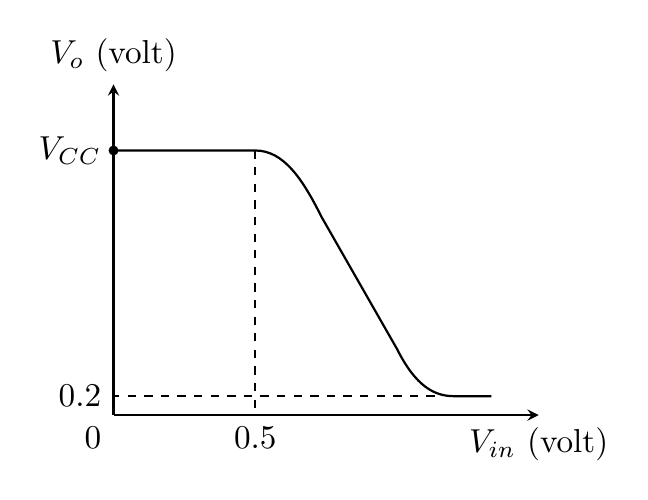
\begin{tikzpicture}[thick,scale=1.2, transform shape]
            
            % Axes
            \draw[->, >=stealth, thick] (0,0) -- (4.5, 0) node[below] {$V_{in}$ (volt)};
            \draw[->, >=stealth, thick] (0,0) -- (0, 3.5) node[above] {$V_o$ (volt)};
            
            % Origin Label
            \node[below left] at (0,0) {0};
            
            % Vcc Dot and Label on Y-axis
            \fill (0, 2.8) circle (1.5pt);
            \node[left] at (0, 2.8) {$V_{CC}$};
            
            % VTC Curve (Cut-off -> Active -> Saturation)
            \draw[thick] (0, 2.8) 
                -- (1.5, 2.8) % Cut-off region (flat)
                .. controls (1.8, 2.8) and (2.0, 2.5) .. (2.2, 2.1) % Curve bending
                -- (3.0, 0.7) % Active region (linear drop)
                .. controls (3.2, 0.3) and (3.4, 0.2) .. (3.6, 0.2) % Curve leveling off
                -- (4.0, 0.2); % Saturation region (flat)
            
            % Dashed Lines for coordinates (0.5 and 0.2)
            \draw[dashed] (1.5, 2.8) -- (1.5, 0) node[below] {0.5};
            \draw[dashed] (3.4, 0.2) -- (0, 0.2) node[left] {0.2};
            
        \end{tikzpicture}
\end{center}
\mk{10} \yr{EEE 263 | L-2/T-1 | 2014--15}

\end{enumerate}


%% ══════════════════════════════════════════════════════════════════════
%%  SECTION 6: MOSFET AMPLIFIERS
%% ══════════════════════════════════════════════════════════════════════
\secdivider{S6 --- MOSFET Amplifiers}{Common-source configuration, small-signal model, gain derivation}{cC}

\markboth{S6: MOSFET Amplifiers}{S6: MOSFET Amplifiers}
\label{sec:S6}
\section*{S6 \quad MOSFET Amplifiers}
\addcontentsline{toc}{section}{S6: MOSFET Amplifiers}

%%──────────────────────────────────────────────────────────────────────
\subtopic{cC}{Common Gate Amplifier}
\label{sub:s6-cg}

\begin{enumerate}\item Derive the expression for input resistance, output resistance, and overall voltage gain of a common-gate (CG) amplifier.
\mk{26} \yr{EEE 263 | L-2/T-1 | 2013--14}

\end{enumerate}

%%──────────────────────────────────────────────────────────────────────
\subtopic{cC}{Common Source Amplifier}
\label{sub:s6-cs}

\begin{enumerate}
    
\item For the Common Source amplifier circuit shown, the transistor has $V_t=1\,\text{V}$, $\mu_n C_{ox}(W/L)=4\,\text{mA/V}^2$, and $V_A=100\,\text{V}$. All capacitors behave as open circuits under DC and short circuits under AC.\\

(i) Find the DC bias voltage $V_D$ and drain current $I_D$ (ignore Early effect for bias). \\
(ii) Find $g_m$, $r_o$ and draw the small-signal equivalent circuit. \\
(iii) Determine $R_{in}$, $R_o$, and the overall voltage gain $v_o/v_{sig}$. \\
(iv) Calculate the maximum peak value of $v_{sig}$ such that $v_{gs} \le 0.1\,V_{OV}$ (small-signal approximation valid). \\
(v) Suggest a circuit modification that will double the maximum $v_{sig}$ found in (iv) without changing the DC bias point.\\
\begin{center}
    \begin{circuitikz}[american, line width=0.8pt,y=1.4cm]
        \ctikzset{tripoles/mos style/arrows}

    % --- MOSFET Transistor ---
    % Positioned at (3, 0) to allow ample space on both sides
    \node[nmos] (M) at (3, 0) {};

    % --- Input Signal Path (Left Side) ---
    % Signal Source vsig
    \draw (-6.5, 0) to[vsource, l=$v_{\text{sig}}$] (-6.5, -2.5) node[ground] {};
    
    % Rsig Resistor
    \draw (-6.5, 0) to[R, l={$R_{\text{sig}}\!=\!200\text{ k}\Omega$}] (-3.5, 0)
          to[short, -o] (-3.0, 0);
          
    % Coupling Capacitor C1
    \draw (-3.0, 0) to[C, l={$C_1\!=\!\infty$}] (-1.0, 0)
          to[short, -o] (-0.5, 0) node[above=4pt] {$v_{gs}$};

    % Wire from vgs node to the Gate bias divider node
    \draw (-0.5, 0) -- (1.5, 0);
    \fill (1.5, 0) circle (2pt);
    \draw (1.5, 0) -- (M.G);

    % Input Resistance Arrow (R_in)
    \draw[->, >=stealth, line width=1.2pt] (0.2, -0.5) -- (1.0, -0.5);
    \node[below] at (0.6, -0.5) {$R_{\text{in}}$};


    % --- Gate Bias Resistors (Voltage Divider) ---
    % Top 10 MOhm Resistor
    \draw (1.5, 0) -- (1.5, 0.4) to[R, l=$10\text{ M}\Omega$] (1.5, 2.8);
    
    % Bottom 5 MOhm Resistor
    \draw (1.5, 0) -- (1.5, -0.4) to[R, l_=$5\text{ M}\Omega$] (1.5, -2.8) node[ground] {};


    % --- Drain Path & Power Supply ---
    \fill (M.D) circle (2pt) node[left=4pt] {$V_D$};
    
    % Drain Resistor (Drawn top-to-bottom to keep ID current arrow pointing down)
    \draw (3, 2.8) to[R, l=$16\text{ k}\Omega$, i=$I_D$] (M.D);
    
    % Power Supply Rail (+15V)
    \draw (1.5, 2.8) -- (3, 2.8);
    \coordinate (VCC) at (2.25, 2.8);
    \fill (VCC) circle (2pt);
    \draw (VCC) to[short, -^] (2.25, 3.5) node[above] {$+15\text{ V}$};


    % --- Source Path & Bypass Capacitor ---
    \draw (M.S) -- (3, -1.0);
    \fill (3, -1.0) circle (2pt);
    
    % Source Resistor 7 kOhm
    \draw (3, -1.0) to[R, l_=$7\text{ k}\Omega$] (3, -3.5) node[ground] {};
    
    % Bypass Capacitor C3
    \draw (3, -1.0) -- (4.8, -1.0)
          to[C, l={$C_3\!=\!\infty$}] (4.8, -3.5) node[ground] {};


    % --- Output Section (Right Side) ---
    % Connection from Drain to C2
    \draw (M.D) -- (4.2, 1.0) 
          to[C, l={$C_2\!=\!\infty$}] (6.2, 1.0);
    \fill (6.2, 1.0) circle (2pt);
    
    % Load Resistor 16 kOhm
    \draw (6.2, 1.0) to[R, l={$16\text{ k}\Omega$}] (6.2, -1.5) node[ground] {};
    
    % Output Terminal vo
    \draw (6.2, 1.0) to[short, -o] (7.8, 1.0) node[right] {$v_o$};

    % Output Resistance Arrow (R_o pointing left)
    \draw[<-, >=stealth, line width=1.2pt] (5.0, 0.5) -- (5.8, 0.5);
    \node[below] at (5.4, 0.5) {$R_o$};


   
\end{circuitikz}
\end{center}
\mk{35} \yr{EEE 263 | L-2/T-1 | 2024--25}

\item Explain why adding a source resistor $R_S$ to a Common-Source MOSFET amplifier improves its bias stability compared to directly grounding the source terminal. Detail how $R_S$ actively compensates for manufacturing variations in the threshold voltage $V_t$ and transconductance parameter $k_n$.
\mk{12} \yr{EEE 263 | L-2/T-1 | 2024--25}

    
\item A CS amplifier is connected to a source $v_{sig}$ with resistance $R_{sig}$ and it utilizes a MOSFET with $\mu_n C_{ox} = 400 \mu\text{A/V}^2$, $W/L = 10$, and $V_A = 10\text{V}$. It is biased at $I_D = 0.2\text{ mA}$ and uses $R_D = 6\text{ k}\Omega$. Find $R_{in}$, $A_{vo}$, and $R_o$. If a load resistance of $10\text{ k}\Omega$ is connected to the output, what will be the overall voltage gain $G_v$? If a 0.2-V peak sine-wave signal is required at the output, what must the peak amplitude of $v_{sig}$ be?
\mk{15} \yr{EEE 263 | L-2/T-1 | 2023--24}



\item In the circuit shown, the NMOS transistor has $|V_t|=0.9\,\text{V}$ and $V_A=50\,\text{V}$ and is operated with $V_D=2\,\text{V}$. What is the voltage gain $v_0/v_i$? What do $V_D$ and the gain become for $I=1\,\text{mA}$?

\begin{center}
      \begin{circuitikz}[thick,scale=1.2, transform shape]
        \ctikzset{tripoles/mos style/arrows}

        % ==========================================
        % Transistor (NMOS)
        % ==========================================
        \draw (0,0) node[nmos] (M) {};
        
        % Source connection to Ground
        \draw (M.S) -- (0, -0.5) node[ground] {};
        
        % ==========================================
        % Drain Branch (Top)
        % ==========================================
        \draw (M.D) -- (0, 2) coordinate (D_node);
        \node at (D_node) {};
        
        % Resistor RD and Positive Supply
        \draw (0.5,4) to[isource, l={$I = 500\ \mu\text{A}$}] (0.5, 2);
        \draw[-latex] (0.5, 4) -- (0.5, 4.7) node[above] {$+V_{DD}$};
        
        % ==========================================
        % Gate and Feedback Resistor (Left)
        % ==========================================
        \draw (M.G) to[short, -*] (-2, 0) coordinate (G_node);
        
        % Feedback Resistor RG connecting Gate and Drain
        \draw (G_node) -- (-2, 2) to[R, l={$R_G = 10\text{ M}\Omega$}] (D_node);
        
        % ==========================================
        % Input Section
        % ==========================================
        % Input Capacitor
        \draw (-4, 0) node[ocirc] (in_term) {} to[C, l_=$\infty$] (G_node);
        
        % Input Voltage (vi) and Ground
        \node at (-4, -0.3) {$+$};
        \draw[-latex] (-4, -0.6) -- (-4, -1.6) node[midway, left] {$v_i$};
        \node at (-4, -1.9) {$-$};
        \draw (-4, -2.2) node[ground] {};
                
        % ==========================================
        % Output Section
        % ==========================================
        % Output Capacitor
        \draw (D_node) to[C, l=$\infty$] (2.5, 2) coordinate (out_node);
        \node[circ] at (out_node) {};
        
        % Load Resistor RL and Ground
        \draw (out_node) to[R, l={$R_L = 10\text{ k}\Omega$}] (2.5, -0.5) node[ground] {};
        
        % Output Terminal (vo)
        \draw (out_node) to[short, -o] (3.5, 2) node[right] {$v_o$};
        
        
    \end{circuitikz}
\end{center}
\mk{17} \yr{EEE 263 | L-2/T-1 | 2022--23}

\item A CS amplifier utilizes a MOSFET biased at $I_D=0.25\,\text{mA}$ with $V_{ov}=0.25\,\text{V}$ and $R_D=20\,\text{k}\Omega$. The amplifier is fed with a signal source having $R_{sig}=100\,\text{k}\Omega$, and a 20-k$\Omega$ load is connected to the output. Find $R_{in}$, $A_{vo}$, $R_o$, $A_v$, and $G_v$.
\mk{20} \yr{EEE 263 | L-2/T-1 | 2021--22}

\item Determine the overall small-signal voltage gain of the common source amplifier shown. The transistor parameters are: $V_t=0.4\,\text{V}$, $k_n=0.5\,\text{mA/V}^2$, $\lambda=0.02\,\text{V}^{-1}$.
\begin{center}
    

    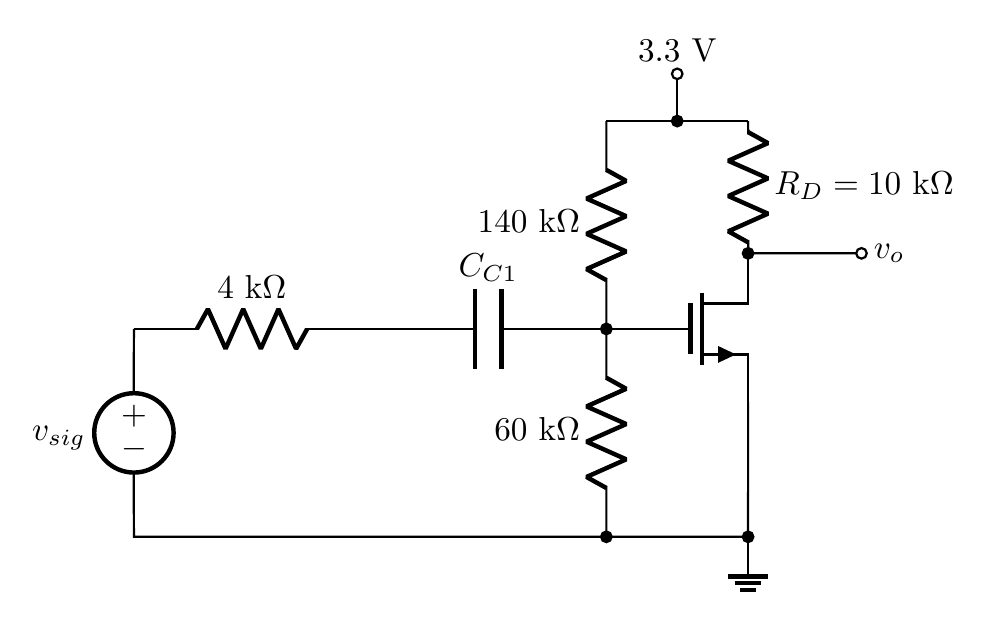
\begin{tikzpicture}[thick,scale=1.2, transform shape]
                              \ctikzset{tripoles/mos style/arrows}

        % 1. NMOS Transistor Setup
        \node[nmos] (Q) at (2, 0) {};
        
        % 2. Gate Node Juncion & Horizontal Input Branch
        % This creates a clean path from v_sig -> 4kOmega -> C_C1 -> Gate
        \draw (-4.5, 0) to[R, l=$4\text{ k}\Omega$] (-2.0, 0) 
                       to[C, l=$C_{C1}$] (0.5, 0) node[circ] (G_junc) {}
                       -- (Q.G);
                       
        % 3. Voltage Divider Network (Vertical Branch at G_junc)
        % Upward to Top Rail
        \draw (G_junc) to[R, l=$140\text{ k}\Omega$] (0.5, 2.2);
        % Downward to Bottom Rail
        \draw (G_junc) to[R, l_=$60\text{ k}\Omega$] (0.5, -2.2) node[circ] {};
        
        % 4. Drain Circuit (Right Side)
        % From Drain up to the node junction for Output (v_o)
        \draw (Q.D) -- (2, 0.8) node[circ] (D_junc) {};
        % Output Node Terminal v_o
        \draw (D_junc) -- (3.2, 0.8) node[ocirc] {} node[right] {$v_o$};
        % Drain Resistor RD going up to Top Rail
        \draw (D_junc) to[R, l_={$R_D = 10\text{ k}\Omega$}] (2, 2.2);
        
        % 5. Top Power Rail (+3.3V)
        \draw (0.5, 2.2) -- (2, 2.2);
        \draw (1.25, 2.2) node[circ] {} -- (1.25, 2.7) node[ocirc] {} node[above] {$3.3\text{ V}$};
        
        % 6. Bottom Ground Rail & Source Connection
        % Direct connection from AC source down to ground rail
        \draw (-4.5, 0) to[V, l_=$v_{sig}$] (-4.5, -2.2) -- (2, -2.2) node[circ] {};
        % Connect NMOS Source straight down to the ground rail
        \draw (Q.S) -- (2, -2.2);
        % Clean Ground Symbol placement below the source node
        \draw (2, -2.2) node[ground] {};
        
    \end{tikzpicture}


\end{center}
\mk{26} \yr{EEE 263 | L-2/T-1 | 2020--21}


\item For the circuit shown, find the small-signal input impedance and voltage gain. Given: $V_t=1.2\,\text{V}$, $k_n'(W/L)=0.5\,\text{mA/V}^2$, and $V_A=55\,\text{V}$.
\begin{center}
    \begin{circuitikz}[thick,american, thick]
          \ctikzset{tripoles/mos style/arrows}

    % --- NMOS Transistor ---
    \node[nmos] (Q) at (0,0) {};

    % --- Source Connection ---
    % Connected directly to ground
    \draw (Q.S) -- (0,-1.5) node[ground] {};

    % --- Drain Connection and Top Bias ---
    % Drain node going upwards
    \draw (Q.D) -- (0,1.5) coordinate (D_node);
    
    % 20k Ohm Resistor and +20V Supply
    \draw (D_node) to[R, l=$20\text{ k}\Omega$] (0,3.5) coordinate (VCC);
    \draw[-stealth] (0,3.5) -- (0,4.2) node[right] {$+20\text{ V}$};

    % --- Feedback Network ---
    % 15M Ohm Resistor connected from drain back to gate
    \draw (D_node) to[R, l=$15\text{ M}\Omega$] (-3,1.5) -- (-3,0) coordinate (G_node);
    \draw (G_node) -- (Q.G);

    % --- Input Network (Left Side) ---
    % Input v_i positive terminal
    \node[ocirc] (Vin_plus) at (-5.5,0) {};
    \node[below=0.1] at (Vin_plus) {$+$};

    % Coupling capacitor with infinity symbol
    \draw (Vin_plus) to[C, l_=$\infty$] (G_node);

    % Input v_i negative terminal and ground
    \node[ocirc] (Vin_minus) at (-5.5,-1.5) {};
    \node[above=0.1] at (Vin_minus) {$-$};
    \draw (Vin_minus) node[ground] {};

    % v_i label between the terminals
    \node at (-5.5,-0.75) {$v_i$};

    % --- Output Network (Right Side) ---
    % Output coupling capacitor with infinity symbol
    \draw (D_node) to[C, l_=$\infty$] (2.5,1.5) coordinate (Out_Junct);
    
    % 25k Ohm Load Resistor to ground
    \draw (Out_Junct) to[R, l=$25\text{ k}\Omega$] (2.5,-1.5) node[ground] {};
    
    % V_o Output terminal
    \draw (Out_Junct) -- (3.5,1.5) node[ocirc] {} node[right] {$V_o$};

    % --- Junction Dots ---
    \filldraw (D_node) circle (1.5pt);     % Drain junction
    \filldraw (G_node) circle (1.5pt);     % Gate junction
    \filldraw (Out_Junct) circle (1.5pt);  % Output junction

\end{circuitikz}
\end{center}
\mk{30} \yr{EEE 263 | L-2/T-1 | Jan--2021}


\item Determine the voltage gain $v_0/v_i$ of the common-source MOSFET amplifier shown in the figure. The transistor has $V_t=1.5\,\text{V}$, $k_n'(W/L)=0.25\,\text{mA/V}^2$, and $V_A=50\,\text{V}$.
\begin{center}
      \begin{circuitikz}[thick,scale=1.2, transform shape]
        \ctikzset{tripoles/mos style/arrows}

        % ==========================================
        % Transistor (NMOS)
        % ==========================================
        \draw (0,0) node[nmos] (M) {};
        
        % Source connection to Ground
        \draw (M.S) -- (0, -0.5) node[ground] {};
        
        % ==========================================
        % Drain Branch (Top)
        % ==========================================
        \draw (M.D) -- (0, 2) coordinate (D_node);
        \node at (D_node) {};
        
        % Resistor RD and Positive Supply
        \draw (0.5,2) to[R, l={$R_D = 10\text{ k}\Omega$}] (0.5, 4);
        \draw[-latex] (0.5, 4) -- (0.5, 4.7) node[above] {$+15\text{ V}$};
        
        % ==========================================
        % Gate and Feedback Resistor (Left)
        % ==========================================
        \draw (M.G) to[short, -*] (-2, 0) coordinate (G_node);
        
        % Feedback Resistor RG connecting Gate and Drain
        \draw (G_node) -- (-2, 2) to[R, l={$R_G = 10\text{ M}\Omega$}] (D_node);
        
        % ==========================================
        % Input Section
        % ==========================================
        % Input Capacitor
        \draw (-4, 0) node[ocirc] (in_term) {} to[C, l_=$\infty$] (G_node);
        
        % Input Voltage (vi) and Ground
        \node at (-4, -0.3) {$+$};
        \draw[-latex] (-4, -0.6) -- (-4, -1.6) node[midway, left] {$v_i$};
        \node at (-4, -1.9) {$-$};
        \draw (-4, -2.2) node[ground] {};
        
        % Input Resistance Arrow (Rin)
        \draw[-latex] (-5, -2.2) -- (-5, -0.8) -- (-4.2, -0.8);
        \node at (-5, -2.5) {$R_{\text{in}}$};
        
        % ==========================================
        % Output Section
        % ==========================================
        % Output Capacitor
        \draw (D_node) to[C, l=$\infty$] (2.5, 2) coordinate (out_node);
        \node[circ] at (out_node) {};
        
        % Load Resistor RL and Ground
        \draw (out_node) to[R, l={$R_L = 10\text{ k}\Omega$}] (2.5, -0.5) node[ground] {};
        
        % Output Terminal (vo)
        \draw (out_node) to[short, -o] (3.5, 2) node[right] {$v_o$};
        
        
    \end{circuitikz}
\end{center}
\mk{20} \yr{EEE 263 | L-2/T-1 | 2017--18}

\item For the circuit shown:
\begin{enumerate}
  \item Calculate DC bias point ($I_D$ and $V_D$).
  \item Draw the small-signal equivalent circuit.
  \item Calculate the small-signal voltage gain.
  \item Find the input resistance.
  \item Determine the largest allowable input signal voltage.
\end{enumerate}
The transistor has $V_t=1.5\,\text{V}$, $k_n'(W/L)=0.25\,\text{mA/V}^2$, and $V_A=50\,\text{V}$.
\begin{center}
  
    \begin{circuitikz}[thick,scale=1.1, transform shape,x=1.6cm]
        \ctikzset{tripoles/mos style/arrows}

        % 1. Input AC Source
        \draw (0,0) node[ground] {} to[sV, l=$v_{in}$] (0,2);
        \node[left] at (-0.3, 2) {$+$};
        \node[left] at (-0.3, 0) {$-$};
        
        % 2. Input Coupling Capacitor & Gate Junction
        \draw (0,2) to[C, l=$\infty$] (2.5,2) coordinate (GateNode);
        \fill (GateNode) circle (1.5pt);
        
        % 3. NMOS Transistor
        \draw (GateNode) -- (3.5,2) node[nmos, anchor=G] (Q) {};
        \draw (Q.S) node[ground] {};
        
        % 4. Feedback Resistor (R_G)
        \draw (GateNode) -- ++(0,1) coordinate (RgLeft) 
              to[R, l={$R_G=10\mathrm{M}\Omega$}] (RgLeft -| Q.D) 
              -- (Q.D);
        
        \fill (Q.D) circle (1.5pt);
        
        % 5. Drain Resistor (R_D) & Power Supply
        \draw (Q.D) -- ++(0,0.5) coordinate (RdBottom) 
              to[R, l_={$R_D=10\mathrm{K}\Omega$}] ++(0,1.5) 
              node[vcc] {$+15\mathrm{V}$};
        
        % 6. Output Coupling Capacitor & Load Resistor (R_L)
        \draw (Q.D) to[C, l=$\infty$] ++(2.5,0) coordinate (OutNode);
        \fill (OutNode) circle (1.5pt);
        
        \draw (OutNode) to[R, l={$R_L=10\mathrm{K}\Omega$}] (OutNode |- 0,0) node[ground] {};
        
        % 7. Output Terminal
        \draw (OutNode) to[short, -o] ++(1,0) node[right] {$v_o$};
        
    \end{circuitikz}
\end{center}
\mk{31} \yr{EEE 263 | L-2/T-1 | 2015--16}

\item For the CS amplifier, derive the expressions for input resistance ($R_{in}$), output resistance ($R_{out}$), open-circuit voltage gain ($A_{vo}$), and overall voltage gain ($G_v$).
\mk{26} \yr{EEE 263 | L-2/T-1 | 2012--13}

\item A common source amplifier circuit is shown in the figure.
\begin{enumerate}
  \item Prove that this circuit is operating in the saturation region.
  \item Draw the small-signal equivalent circuit.
  \item Find $g_m$, $R_{in}$, $R_{out}$, $A_v$, and $G_v$.
\end{enumerate}
Assume $V_t=1\,\text{V}$, $K_n' W/L=2\,\text{mA/V}^2$, $V_A=100\,\text{V}$.


\begin{center}
\begin{circuitikz}[thick,american, thick, scale=1.1, transform shape]
                      \ctikzset{tripoles/mos style/arrows}

  % ==========================================
  % NMOS Transistor
  % ==========================================
  \draw (3,3) node[nmos] (Q) {};
  % Source pin er upore nicher dike mukh kora arrow (n-channel er jonnno)

  % ==========================================
  % Gate Bias (Voltage Divider)
  % ==========================================
  % R_G1 (Upper) and R_G2 (Lower)
  \draw (1.5, 6) to[R, l_={ $10\text{ M}\Omega$ }] (1.5, 3)
        to[R, l_={ $5\text{ M}\Omega$ }] (1.5, 0) node[ground]{};
  
  % Connection to Gate
  \draw (1.5, 3) -- (Q.G);
  \draw[fill=black] (1.5, 3) circle (1.5pt);

  % ==========================================
  % VDD (+15 V) Rails
  % ==========================================
  \draw[-stealth] (1.5, 6) -- (1.5, 6.8);
  \draw[-stealth] (3, 6) -- (3, 6.8);
  \node[above] at (2.25, 6.8) {$+15\text{ V}$};

  % ==========================================
  % Drain & Source Branches
  % ==========================================
  % Drain Resistor
  \draw (Q.D) to[R, l_={ $7.5\text{ k}\Omega$ }] (3, 6);
  \draw[fill=black] (Q.D) circle (1.5pt);
  
  % Source Resistor
  \draw (Q.S) to[R, l_={ $3\text{ k}\Omega$ }] (Q.S |- 0,0) node[ground]{};
  \draw[fill=black] (Q.S) circle (1.5pt);
  
  % Source Bypass Capacitor
  \draw (Q.S) -- ++(1.5,0) coordinate (CS) 
        to[C, l_={ $\infty$ }] (CS |- 0,0) node[ground]{};

  % ==========================================
  % Input Section (v_sig, R_sig, C_in)
  % ==========================================
  % AC Voltage Source
  \draw (-4.5, 3) to[V, l={ $v_{\text{sig}}$ }] (-4.5, 0) node[ground]{};
  
  % Series Resistor with open terminal (-o)
  \draw (-4.5, 3) to[R, l={ $R_{\text{sig}} = 100\text{ k}\Omega$ }, -o] (-1.5, 3);
  
  % Input Coupling Capacitor with open terminal (-o)
  \draw (-1.5, 3) to[C, l={ $\infty$ }, -o] (0.5, 3);
  
  % v_gs node label and connection to gate
  \node[above] at (0.5, 3.1) {$v_{gs}$};
  \draw (0.5, 3) -- (1.5, 3);

  % R_in pointing arrow
  \draw[-stealth] (-0.2, 0) node[below]{$R_{\text{in}}$} |- (1.3, 2.7);

  % ==========================================
  % Output Section (C_out, R_L)
  % ==========================================
  % Output Coupling Capacitor
  \draw (Q.D) to[C, l={ $\infty$ }] ++(2.5,0) coordinate (CD_end);
  
  % Output terminal
  \draw (CD_end) to[short, -o] ++(1,0) node[right]{$v_o$};
  \draw[fill=black] (CD_end) circle (1.5pt);
  
  % Load Resistor to ground
  \draw (CD_end) to[R, l={ $10\text{ k}\Omega$ }] (CD_end |- 0,0) node[ground]{};

\end{circuitikz}
\end{center}


\mk{46} \yr{EEE 263 | L-2/T-1 | 2011--12}


\end{enumerate}


%% ══════════════════════════════════════════════════════════════════════
%%  PART IV
%% ══════════════════════════════════════════════════════════════════════
\secdivider{Part IV --- Linear Integrated Circuits}{Op-amp ideal characteristics, mathematical operations, active filters, ADC}{cE}

%%──────────────────────────────────────────────────────────────────────\n\subtopic{cC}{Source Resistor and Bias Stability}

%% ══════════════════════════════════════════════════════════════════════
%%  SECTION 7: OPERATIONAL AMPLIFIERS
%% ══════════════════════════════════════════════════════════════════════
\markboth{S7: Operational Amplifiers}{S7: Operational Amplifiers}
\label{sec:S7}
\titleformat{\section}{\large\bfseries\color{cE}}{}{0em}{}[\titlerule]
\section*{S7 \quad Operational Amplifiers (Op-Amps)}
\addcontentsline{toc}{section}{S7: Operational Amplifiers}

%%──────────────────────────────────────────────────────────────────────
\subtopic{cE}{Ideal Op-Amp Characteristics}
\label{sub:s7-ideal}

\begin{enumerate}\item What are the characteristics of an ideal op-amp?
\mk{5} \yr{EEE 263 | L-2/T-1 | 2013--14}

\item Explain graphically why in a closed-loop feedback circuit of an Op-Amp the differential voltage $E_d$ is taken as zero.
\mk{12} \yr{EEE 263 | L-2/T-1 | 2012--13}

\item Derive the closed-loop gain of an inverting Op-Amp amplifier as a function of its open-loop gain, provided that the open-loop gain is not infinity.
\mk{13} \yr{EEE 263 | L-2/T-1 | 2012--13}

\item Write down the properties of an ideal Op-Amp.
\mk{10} \yr{EEE 263 | L-2/T-1 | 2011--12}

\end{enumerate}

%%──────────────────────────────────────────────────────────────────────
\subtopic{cE}{Mathematical Operations}
\label{sub:s7-math}

\begin{enumerate}

\item For the circuit shown in Figure below, find all the marked node voltages and branch currents:

\begin{center}
    \begin{circuitikz}[thick, scale=1.2, transform shape]

    % Op-amp placed at coordinate (1.5, 0)
    \node[op amp] (opamp) at (1.5,0) {};

    % Inverting input node
    \draw (0, 0.5) node[circ] (NodeA) {} -- (opamp.-);

    % Non-inverting input to ground
    \draw (opamp.+) -- ++(-0.5,0) to[short] ++(0,-0.5) node[ground] {};

    % Input branch and voltage source
    \draw (-3, 0.5) node[ocirc] (VinNode) {} to[R, l_=$1\,\text{k}\Omega$, i^=$i_1$] (NodeA);
    \draw (-3, -1.5) node[ground] {} to[V,invert,  l_=$5\,\text{V}$] (VinNode);
    \node[left] at (-3.7, -0.5) {$v_{\text{in}}$};

    % Feedback Network (T-network)
    % Left vertical wire
    \draw (NodeA) to[short, i^=$i_2$] (0, 2.5);

    % Top-left horizontal resistor
    \draw (0, 2.5) to[R, l_=$1\,\text{k}\Omega$] (2.5, 2.5) node[circ] (NodeB) {};

    % Middle grounded resistor
    \draw (2.5, 0.8) node[ground] {} to[R, l^=$1\,\text{k}\Omega$, i_=$i_3$] (NodeB);

    % Top-right horizontal resistor
    \draw (NodeB) to[R, l_=$1\,\text{k}\Omega$] (5, 2.5);

    % Right vertical wire
    \draw (5, 2.5) to[short, i^=$i_4$] (5, 0);

    % Connect to op-amp output
    \draw (opamp.out) -- (5, 0) node[circ] {};

    % Output terminals (v_0)
    \draw (5, 0) -- (6, 0) node[ocirc] (Vout+) {};
    \draw (6, -1.5) node[ocirc] (Vout-) {} -- (6, -2) node[ground] {};
    
    % This draws the +, - and v_0 label automatically between the two open nodes
    \draw (Vout+) to[open, v=$v_0$] (Vout-);

\end{circuitikz}

\end{center}
\mk{17} \yr{EEE 263 | L-2/T-1 | 2023--24}

\item Suppose, you have three voltage sources: $V_1 = \sin(40t)$, $V_2 = \sin(100t)$, $V_3 = 1\text{V}$. Design a circuit using op-amps that will generate the following output:
$$V_{out} = 5\sin(40t) - 4\cos(100t) + 4$$
Draw the overall connection diagram with required values of elements. You may assume that the op-amps are biased using a 15V source.   
\mk{18} \yr{EEE 263 | L-2/T-1 | 2023--24}


\item Find the expression of output voltage $v_0$ in terms of input voltages and resistances in the circuit shown. Also calculate the value of output voltage at $t=1\,\text{sec}$ given that $v_1=2\,\text{V}$, $v_2=5\,\text{V}$, $v_3=1\,\text{V}$, and $v_4=5\sin(100\pi t)$.
\begin{center}
    
\begin{circuitikz}[thick,american, scale=1.2, thick]

    % ==========================================
    % First Op-Amp Stage
    % ==========================================
    \node[op amp] (op1) at (0,0) {};
    
    % Inverting Input (-) Node for Op-Amp 1
    \coordinate (in_node1) at ($(op1.-) + (-0.5,0)$);
    \draw (op1.-) -- (in_node1);
    \node[circ] at (in_node1) {};
    
% v1 Input Branch
\draw (in_node1) 
to[R, l_=$1\text{ k}\Omega$] ++(-2.5,0) 
node[ocirc] {} 
node[left] {$v_1$};

% v2 Input Branch
\draw (in_node1) -- ++(0,-0.5) 
to[R, l=$5\text{ k}\Omega$] ++(-2.5,0) 
node[ocirc] {} 
node[left] {$v_2$};
    
    % Non-inverting Input (+) and Ground for Op-Amp 1
    \coordinate (pos1_node) at ($(op1.+) + (-0.5,0)$);
    \draw (op1.+) -- (pos1_node) -- ++(0,-0.8) node[ground] {};
    
    % Feedback Path for Op-Amp 1
    \coordinate (out1) at (op1.out);
    \coordinate (fb1_left) at ($(in_node1) + (0, 1.5)$);
    \draw (in_node1) -- (fb1_left) to[R, l=$5\text{ k}\Omega$] (fb1_left -| out1) -- (out1);
    \node[circ] at (out1) {};
    
    % ==========================================
    % Second Op-Amp Stage
    % Offset downwards so its '-' input perfectly aligns horizontally with out1
    % ==========================================
    \node[op amp] (op2) at (6.5, -0.5) {}; 
    
    % Interstage Connection
    \coordinate (in_node2) at ($(op2.-) + (-0.5,0)$);
    \draw (out1) to[R, l=$1\text{ k}\Omega$] (in_node2);
    \draw (in_node2) -- (op2.-);
    \node[circ] at (in_node2) {};
    
    % Inverting Input (-) vertical line to Feedback and v3
    \coordinate (top_node2) at ($(in_node2) + (0, 1.5)$);
    \draw (in_node2) -- (top_node2);
    \node[circ] at (top_node2) {};
    
    % v3 Input Branch
    \draw (top_node2) to[R, l=$500\,\Omega$] ++(-2.5,0) node[ocirc] {} node[left] {$v_3$};
    
    % Feedback Path for Op-Amp 2
    \coordinate (out2) at (op2.out);
    \draw (top_node2) to[R, l=$1\text{ k}\Omega$] (top_node2 -| out2) -- (out2);
    \node[circ] at (out2) {};
    
    % Non-inverting Input (+) for Op-Amp 2, v4, and Ground
    \coordinate (pos2_node) at ($(op2.+) + (-0.5,0)$);
    \draw (op2.+) -- (pos2_node);
    \node[circ] at (pos2_node) {};
    \draw (in_node2) to[R, l=$500\,\Omega$] ++(-2.5,-2) node[ocirc] {} node[left] {$v_4$};
    \draw (pos2_node) -- ++(0,-0.8) node[ground] {};
    
    % ==========================================
    % Output Terminal and Caption
    % ==========================================
    \draw (out2) -- ++(1.5,0) node[ocirc] {} node[right] {$v_o$};
    
\end{circuitikz}
\end{center}
\mk{20} \yr{EEE 263 | L-2/T-1 | 2018--19}

\item For the circuit shown, find $V_0$. The MOSFET is in saturation with $k_n'(W/L)=1\,\text{mA/V}^2$ and $V_t=0.7\,\text{V}$. The op-amp is ideal.
\begin{center}
  
\begin{circuitikz}[thick,american, scale=1.2]
    \ctikzset{tripoles/mos style/arrows}

    % 1. Place the Operational Amplifier
    \node[op amp] (OA) at (0,0) {};
    
    % 2. Power Supply Rails for the Op-Amp
    \draw (OA.up) -- ++(0,0.3) node[above] {$+15\text{V}$};
    \draw (OA.down) -- ++(0,-0.3) node[below] {$-15\text{V}$};
    
    % 3. Non-inverting input (+) connected to Ground
    \draw (OA.+) -- ++(0,-0.4) node[ground] {};
    
    % 4. Inverting input (-) connection and Input Resistor
    \draw (OA.-) -- ++(-0.6,0) coordinate (FB) 
          to[R, l_=$1\text{ k}\Omega$, *-] ++(-2.5,0) 
          node[circle, fill, inner sep=1pt]{} node[left] {$2\text{V}$};
          
    % 5. Place the NMOS Transistor aligned with the Op-Amp output
    \node[nmos, anchor=source] (MOS) at (3.2, 0) {};
    
    % 6. Connect Op-Amp Output to MOSFET Source (S)
    \draw (OA.out) -- (MOS.source) 
          node[left, pos=0.85,circ] {S} 
          node[below, pos=1.0] {$V_o$};
          
    % 7. Connect MOSFET Gate (G) to Ground
    \draw (MOS.gate) -- ++(-0.3,0) node[ground] {} 
          node[above left] {G};
          
    % 8. Feedback Loop from Inverting Input to MOSFET Drain (D)
    \draw (FB) -- ++(0,1.3) 
          to[R, l=$1\text{K}$, i^>=$I_D$] (3.2, 1.8) 
          -- (MOS.drain) 
          node[right, pos=0.5] {D};
          
    % 9. Figure Caption/Label
    \node[below] at (0.8,-1.8) {Fig for Q. 5(a)};

\end{circuitikz}
\end{center}
\mk{10} \yr{EEE 263 | L-2/T-1 | 2017--18}

\item Consider the circuit and input voltage waveform shown in the figure. (i) If $R=10\,\text{k}\Omega$, $C=0.1\,\mu\text{F}$, and the Op-Amp is ideal, sketch the output voltage waveform to scale. (ii) If $R=10\,\text{k}\Omega$, what value of $C$ is required for the peak-to-peak output amplitude to be 2\,V?
\begin{center}

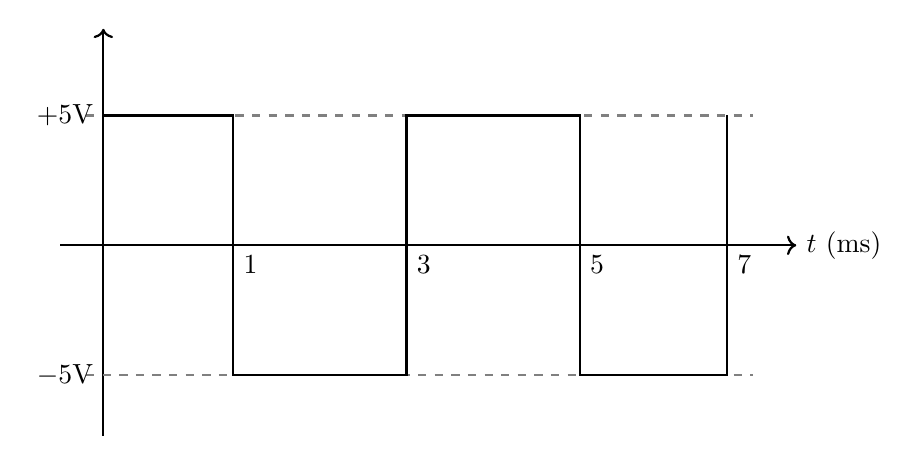
\begin{tikzpicture}[thick,american, scale=1.1]

        \draw[->, thick] (-0.5,0) -- (8.0,0) node[right] {$t\text{ (ms)}$};
        \draw[->, thick] (0,-2.2) -- (0,2.5);
        
        % Dashed horizontal voltage reference levels
        \draw[dashed, gray] (-0.2, 1.5) -- (7.5, 1.5);
        \draw[dashed, gray] (-0.2, -1.5) -- (7.5, -1.5);
        
        % Y-Axis Labels
        \node[left] at (0, 1.5) {$+5\text{V}$};
        \node[left] at (0, -1.5) {$-5\text{V}$};
        
        % Square Waveform
        \draw[thick] (0, 1.5) -- (1.5, 1.5) 
                  -- (1.5, -1.5) -- (3.5, -1.5) 
                  -- (3.5, 1.5) -- (5.5, 1.5) 
                  -- (5.5, -1.5) -- (7.2, -1.5)
                  -- (7.2, 1.5);
        
        % X-Axis Time Markers
        \node[below right] at (1.5, 0) {$1$};
        \node[below right] at (3.5, 0) {$3$};
        \node[below right] at (5.5, 0) {$5$};
        \node[below right] at (7.2, 0) {$7$};
  \end{tikzpicture}
\end{center}
\begin{center}
  
 \begin{circuitikz}[thick,american, scale=1.1]

        % Operational Amplifier
        \node[op amp] (OA) at (0,0) {};
        
        % Power Supply Rails
        \draw (OA.up) -- ++(0,0.3) node[above] {$+15$};
        \draw (OA.down) -- ++(0,-0.3) node[below] {$-15$};
        
        % Non-inverting input (+) to Ground
        \draw (OA.+) -- ++(0,-0.4) node[ground] {};
        
        % Inverting input (-) connection node
        \draw (OA.-) -- ++(-0.4,0) coordinate (FB_left);
        
        % Input Resistor (R) and Vin Terminals
        \draw (FB_left) to[R, l_=$R$] ++(-2.0,0) coordinate (Vin_top);
        \draw (Vin_top) node[circle, draw, inner sep=1pt] {} node[above=2pt] {$+$};
        \node[below=25pt] (Vin_gnd) at (Vin_top) {};
        \draw (Vin_gnd.center) node[ground] {} node[below=2pt] {$-$};
        \node at ($(Vin_top)!0.5!(Vin_gnd)$) {$V_{in}$};
        
        % Output Nodes
        \draw (OA.out) -- ++(0.6,0) coordinate (FB_right);
        \draw (FB_right) -- ++(0.5,0) coordinate (Vout_top);
        \draw (Vout_top) node[circle, draw, inner sep=1pt] {} node[right=4pt] {$+V_o$};
        \node[below=25pt] (Vout_gnd) at (Vout_top) {};
        \draw (Vout_gnd.center) node[ground] {} node[right=4pt] {$-$};
        
        % Feedback Branch 1: Capacitor (C)
        \draw (FB_left) -- ++(0,1.1) coordinate (C_left)
              to[C, l=$C$] (FB_right |- C_left) -- (FB_right);
              
        % Feedback Branch 2: Reset Switch (t=0)
        \draw (C_left) -- ++(0,0.8) coordinate (SW_left)
              to[closing switch, l={$t=0$}] (FB_right |- SW_left) -- (FB_right |- C_left);
    
    

\end{circuitikz}
\end{center}
\mk{16} \yr{EEE 263 | L-2/T-1 | 2017--18}

\item For the circuit shown, (i) determine output voltage $V_{out}$ in terms of input voltage $V_{in}$; (ii) using this circuit perform the following operation: $V_{out} = 3V_{in}^2$. Use additional Op-Amps and a DC voltage source if necessary. Specify values of all the parameters used. (Threshold voltage $V_{TH}=0.5\,\text{V}$ for the MOSFET M1.)
\begin{center}
  
    \begin{circuitikz}[thick,scale=1.2, transform shape]
                \ctikzset{tripoles/mos style/arrows}

        % Op-amp
        \draw (0,0) node[op amp] (opamp) {};
        
        % Power Supplies (with arrows as in the image)
        \draw[->] (opamp.up) -- ++(0,0.5) node[above] {$+ 15\mathrm{\ V}$};
        \draw[->] (opamp.down) -- ++(0,-0.5) node[below] {$- 15\mathrm{\ V}$};
        
        % Non-inverting Input (+)
        \draw (opamp.+) -- ++(-0.5,0) node[ground] {};
        
        % Inverting Input (-) and Vin Source
        \draw (opamp.-) coordinate (in_minus) 
              to[R, l_=$R$] ++(-2.5,0) coordinate (v_in_top)
              to[V, l=$V_{\mathrm{in}}$] ++(0,-2) node[ground] {};
        
        % Output Node
        \draw (opamp.out) -- ++(0.5,0) coordinate (out_node)
              to[short, -o] ++(1,0) node[right] {$V_{\mathrm{out}}$};
              
        % MOSFET M1
        \draw (out_node) ++(1, 1.5) node[nmos] (M1) {};
        \node at ([xshift=0.4cm]M1.east) {$M_1$};
        
        % Connections for M1
        \draw (out_node) -- (M1.S);
        \draw (M1.G) -- ++(-0.5,0) node[ground] {};
        \draw (M1.D) -- ++(0,0.5) -| (in_minus);
        
        % Junction dots
        \fill (in_minus) circle(1.5pt);
        \fill (out_node) circle(1.5pt);
        
    \end{circuitikz}
\end{center}
\mk{20} \yr{EEE 263 | L-2/T-1 | 2015--16}

\item What is the value of the output voltage $V_o$ for the circuit shown?
\begin{center}
      \begin{circuitikz}[thick,scale=1.2, transform shape]
        
        % ১. Op-Amp (Operational Amplifier)
        % \node[op amp] ব্যবহার করলে ডিফল্টভাবে ইনভার্টিং (-) উপরে এবং নন-ইনভার্টিং (+) নিচে থাকে
        \node[op amp] (OA) at (0,0) {};
        
        % ২. Power Supplies (+15V এবং -15V)
        \draw (OA.up) -- ++(0, 0.5) node[above] {$+15\mathrm{V}$};
        \draw (OA.down) -- ++(0, -0.5) node[below] {$-15\mathrm{V}$};
        
        % ৩. Inverting (-) Terminal & Feedback Loop
        \draw (OA.-) -- ++(-0.5, 0) coordinate (inv); % Junction point
        % 2K Resistor and 2V input
        \draw (inv) to[R, l_=$2\mathrm{K}$, -*] ++(-2, 0) node[left] {$2\mathrm{V}$};
        
        % 5K Feedback Resistor
        \draw (inv) to[short, *-] ++(0, 1.5) coordinate (fb_left)
              to[R, l=$5\mathrm{K}$] (fb_left -| OA.out) coordinate (fb_right)
              to[short, -*] (OA.out);
        
        % ৪. Non-Inverting (+) Terminal
        \draw (OA.+) -- ++(-0.5, 0) coordinate (noninv); % Junction point
        % 3K Resistor and 7V input
        \draw (noninv) to[R, l_=$3\mathrm{K}$, -*] ++(-2, 0) node[left] {$7\mathrm{V}$};
        % 4K Resistor to Ground
        \draw (noninv) to[R, l=$4\mathrm{K}$, *-] ++(0, -1.8) node[ground]{};
        
        % ৫. Output Terminal (Vo)
        \draw (OA.out) to[short, -*] ++(1, 0) node[right] {$V_o$};
        
    \end{circuitikz}
\end{center}
\mk{16.67} \yr{EEE 263 | L-2/T-1 | 2014--15}

\item Design an Op-Amp circuit that performs the following mathematical operation:
\[
v_{out} = 5v_1 - 2\frac{dv_2}{dt} + 6\int v_3\,dt
\]
where $v_1$, $v_2$, and $v_3$ are three input signals and $v_{out}$ is the overall output signal.
\mk{16} \yr{EEE 263 | L-2/T-1 | 2012--13}

\item Propose a circuit using Op-Amp which will produce the following as output:
\[
V_{out} = -4V_1 + 2V_2 + 7\frac{dV_1}{dt} - 8\int V_2\,dt
\]
where $V_1$ and $V_2$ are two different input sources.
\mk{20} \yr{EEE 263 | L-2/T-1 | 2011--12}

\end{enumerate}

%%──────────────────────────────────────────────────────────────────────
\subtopic{cE}{Logarithmic / Exponential Amplifier}
\label{sub:s7-log}


\begin{enumerate}
    

\item For the circuit shown , deduce the equation for output voltage $V_0$ and explain the function of this circuit.
\begin{center}
    \begin{circuitikz}[thick,american, thick]

    % --- Operational Amplifier ---
    \node[op amp] (opamp) at (0,0) {};

    % --- Inverting Input (-) Network ---
    % Create a junction node to the left of the inverting input
    \coordinate (in_node) at ($(opamp.-) + (-0.5,0)$);
    \draw (opamp.-) -- (in_node);
    \filldraw (in_node) circle (1.5pt);

    % Diode and Input Terminal
    % Diode D pointing towards the op-amp
    \draw ($(in_node) + (-2.5,0)$) node[left] {$V_i$} to[D, l=D, *-] (in_node);

    % --- Non-inverting Input (+) Network ---
    % Connected to ground
    \draw (opamp.+) -- ++(-0.5,0) -- ++(0,-0.5) node[ground] {};

    % --- Feedback Network ---
    % Feedback Resistor Rf from inverting input junction to output
    \draw (in_node) -- ++(0,1.5) coordinate (fb_left)
          to[R, l=$R_f$] (fb_left -| opamp.out) coordinate (fb_right)
          -- (opamp.out);

    % --- Output Network ---
    % Junction dot at the output where feedback connects
    \filldraw (opamp.out) circle (1.5pt); 
    
    % Output terminal Vo
    \draw (opamp.out) to[short, -*] ++(1.5,0) node[right] {$V_o$};
    

\end{circuitikz}
\end{center}
\mk{17} \yr{EEE 263 | L-2/T-1 | Jan--2021}    
    
    \item Show that a proper connection of a diode, a resistor, and an op-amp can perform the exponential function. Mention the assumptions, if any.
\mk{Unspecified} \yr{EEE 263 | L-2/T-1 | 2013--14}

\item Draw the circuit diagram of an inverting logarithmic amplifier and derive the expression of its output voltage.
\mk{26} \yr{EEE 263 | L-2/T-1 | 2011--12}

\end{enumerate}

%%──────────────────────────────────────────────────────────────────────
\subtopic{cE}{Difference Amplifier}
\label{sub:s7-diff}

\begin{enumerate}\item Design a subtractor circuit using op-amps so that the output voltage is $v_0 = v_1 - v_2$.
\mk{15} \yr{EEE 263 | L-2/T-1 | 2022--23}

\item Design a circuit using a single Op-Amp that performs the following operation: $V_o = 3(V_1 - V_2)$ where $V_1$ and $V_2$ are input signals (AC or DC). Specify values of all resistors used in the design.
\mk{14} \yr{EEE 263 | L-2/T-1 | 2015--16}

\item Implement $z = 5V_1 - 3V_2$ using only one op-amp, where $V_1$ and $V_2$ are input signals.
\mk{15} \yr{EEE 263 | L-2/T-1 | 2013--14}

\end{enumerate}

%%──────────────────────────────────────────────────────────────────────
\subtopic{cE}{Comparator and Schmitt Trigger}
\label{sub:s7-schmitt}

\begin{enumerate}


\item Write down the characteristics of an ideal op-amp. Draw the voltage transfer characteristics of the circuit shown in Figure below. Voltage transfer characteristics shows the variation in output voltage in response to variations in the input voltage.
\begin{center}
\begin{circuitikz}[thick, scale=1, transform shape]
    % Op-amp with non-inverting (+) input on top, filled with gray
    \draw (3,0) node[op amp, noinv input up] (opamp) {}; 
    
    % Inverting (-) terminal to ground
    \draw (opamp.-) -- ++(0,-0.5) node[ground] {};
    
    % Non-inverting (+) terminal node
    \draw (opamp.+) to[short, -*] ++(-0.5,0) coordinate (Vplus) node[below left] {V\textsubscript{+}};
    
    % Input resistor R1 and Voltage Source Vin
    \draw (Vplus) to[R, l_=$R_1$] ++(-2.5,0) coordinate (V_in_top);
    \draw (V_in_top) to[V, v_=$\text{V}_{\text{in}}$] ++(0,-1.5) node[ground] {};
    
    % Positive feedback resistor R2
    \draw (Vplus) -- ++(0, 1.2) coordinate (up) to[R, l=$R_2$] (up -| opamp.out) to[short, -*] (opamp.out);
    
    % Output node Vo
    \draw (opamp.out) to[short, -o] ++(1,0) node[right] {V\textsubscript{o}};
\end{circuitikz}
\end{center}

\mk{15} \yr{EEE 263 | L-2/T-1 | 2023--24}

    
\item Determine the op-amp circuit that generates the transfer characteristics shown in the figure.
\begin{center}
  
    \begin{tikzpicture}[thick,x=1.5cm, y=1cm]
        
        % Draw axes
        \draw[->, thick] (-2.5, 0) -- (2, 0) node[right] {$V_{in}$};
        \draw[->, thick] (0, -2.5) -- (0, 3.5) node[above] {$V_{out}$};
        
        % Draw the hysteresis loop lines
        % Lower horizontal trace
        \draw[thick] (-2.2, -1.2) -- (-1.5, -1.2);
        
        % Upper horizontal trace
        \draw[thick] (-1.5, 2.2) -- (1.5, 2.2);
        
        % Left vertical transition
        \draw[thick] (-1.5, -1.2) -- (-1.5, 2.2);
        
        % Right vertical transition (along the y-axis)
        
        % Dashed line extending for the -12V label
        \draw[dashed, thick] (-1.5, -1.2) -- (0.8, -1.2);
        
        % Voltage level labels
        \node[above right] at (0, 2.2) {$+22$V};
        \node[below right] at (0, -1.2) {$-12$V};
        \node[below left] at (-1.5, 0) {$-8$V};
                
    \end{tikzpicture}
\end{center}
\mk{11} \yr{EEE 263 | L-2/T-1 | 2016--17}

\item Design a Schmitt trigger that triggers from $+16\,\text{V}$ to $-16\,\text{V}$ at an input voltage of 12\,V and triggers from $-16\,\text{V}$ to $+16\,\text{V}$ at an input voltage of 8\,V. Specify all the values of resistors and reference DC voltage.
\mk{15} \yr{EEE 263 | L-2/T-1 | 2014--15}

\item Draw a zero-crossing detector circuit using Op-Amp and briefly describe its operation.
\mk{15} \yr{EEE 263 | L-2/T-1 | 2012--13}

\end{enumerate}

%%──────────────────────────────────────────────────────────────────────
\subtopic{cE}{Waveform Generation}
\label{sub:s7-wave}

\begin{enumerate}\item Design a circuit using op-amp(s) for given input $v_i(t)$ and output $v_o(t)$ waveforms shown in the figure.
\begin{center}
    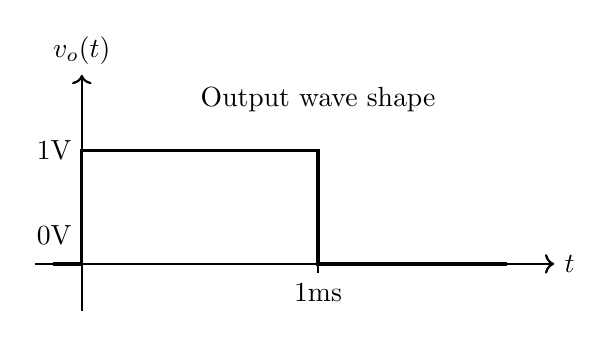
\begin{tikzpicture}[thick,scale=1.2]

        % Axes
        \draw[->, thick] (-0.5, 0) -- (5, 0) node[right] {$t$};
        \draw[->, thick] (0, -0.5) -- (0, 2) node[above] {$v_o(t)$};
        
        % Y-axis labels
        \node[left] at (0,0.3) {$0\text{V}$};
        \node[left] at (0,1.2) {$1\text{V}$};
        
        % X-axis ticks
        \draw[thick] (2.5, 0.1) -- (2.5, -0.1) node[below] {$1\text{ms}$};
        
        % Waveform (thick line)
        \draw[very thick] (-0.3, 0) -- (0, 0) -- (0, 1.2) -- (2.5, 1.2) -- (2.5, 0) -- (4.5, 0);
        
        % Plot Title
        \node[above] at (2.5, 1.5) {Output wave shape};


\end{tikzpicture}
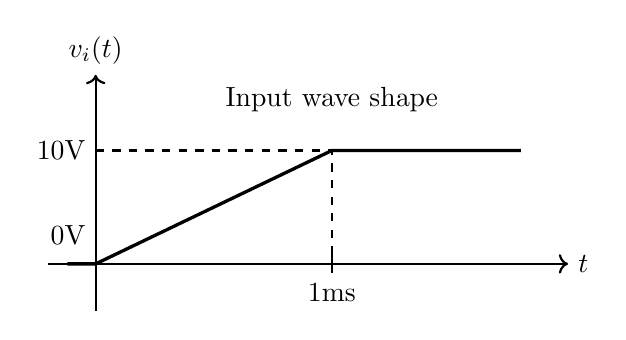
\begin{tikzpicture}[thick,scale=1.2]
        % Axes
        \draw[->, thick] (-0.5, 0) -- (5, 0) node[right] {$t$};
        \draw[->, thick] (0, -0.5) -- (0, 2) node[above] {$v_i(t)$};
        
        % Y-axis labels
        \node[left] at (0,0.3) {$0\text{V}$};
        \node[left] at (0,1.2) {$10\text{V}$};
        
        % X-axis ticks
        \draw[thick] (2.5, 0.1) -- (2.5, -0.1) node[below] {$1\text{ms}$};
        
        % Dashed helper lines
        \draw[dashed] (0, 1.2) -- (2.5, 1.2) -- (2.5, 0);
        
        % Waveform (thick line)
        \draw[very thick] (-0.3, 0) -- (0, 0) -- (2.5, 1.2) -- (4.5, 1.2);
        
        % Plot Title
        \node[above] at (2.5, 1.5) {Input wave shape};

\end{tikzpicture}
\end{center}
\mk{16} \yr{EEE 263 | L-2/T-1 | 2018--19}

\item Input signal $V_{in}$ and output signal $V_{out}$ of a circuit are given in the figure. Design the circuit using Op-Amps. Show necessary calculations.
\begin{center}
    % ==========================================
    % প্রথম গ্রাফ: Vin (Triangle Wave)
    % ==========================================
    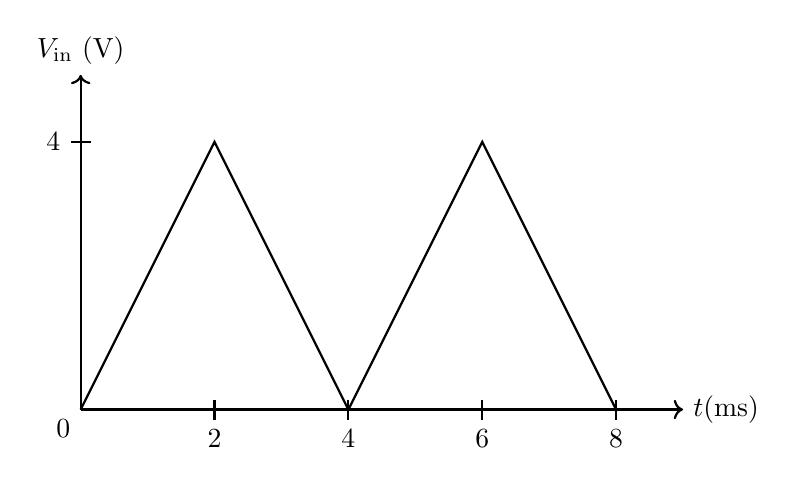
\begin{tikzpicture}[thick,scale=0.85]
        % Axes
        \draw[->, thick] (0,0) -- (9,0) node[right] {$t(\mathrm{ms})$};
        \draw[->, thick] (0,0) -- (0,5) node[above] {$V_{\mathrm{in}}\ (\mathrm{V})$};

        % X-axis Ticks and Labels
        \foreach \x in {2,4,6,8} {
            \draw (\x, 0.15) -- (\x, -0.15) node[below] {\x};
        }
        % Y-axis Ticks and Labels
        \draw (0.15, 4) -- (-0.15, 4) node[left] {4};
        \node[below left] at (0,0) {0};

        % Triangle Waveform
        \draw[thick] (0,0) -- (2,4) -- (4,0) -- (6,4) -- (8,0);
    \end{tikzpicture}
    \hspace{1cm} % দুটি গ্রাফের মাঝে ফাঁকা জায়গা
    % ==========================================
    % দ্বিতীয় গ্রাফ: Vout (Square Wave)
    % ==========================================
    \begin{tikzpicture}[thick,scale=0.85]
        % Axes
        \draw[->, thick] (0,0) -- (9,0) node[right] {$t(\mathrm{ms})$};
        \draw[->, thick] (0,-3) -- (0,3) node[above] {$V_{\mathrm{out}}\ (\mathrm{V})$};

        % X-axis Ticks and Labels
        \foreach \x in {2,4,6,8} {
            \draw (\x, 0.15) -- (\x, -0.15) node[below] {\x};
        }
        % Y-axis Ticks and Labels
        \draw (0.15, 2) -- (-0.15, 2) node[left] {2};
        \draw (0.15, -2) -- (-0.15, -2) node[left] {-2};
        \node[below left] at (0,0) {0};

        % Square Waveform
        \draw[thick] (0,2) -- (2,2) -- (2,-2) -- (4,-2) -- (4,2) -- (6,2) -- (6,-2) -- (8,-2) -- (8,2);
    \end{tikzpicture}
\end{center}
\mk{12} \yr{EEE 263 | L-2/T-1 | 2015--16}

\item Design a circuit using Op-Amps that gives a specified output waveform from a 1\,V DC input. Use $+15\,\text{V}$ and $-15\,\text{V}$ for DC biasing. Specify all the values of resistors and capacitors used.
\begin{center}
      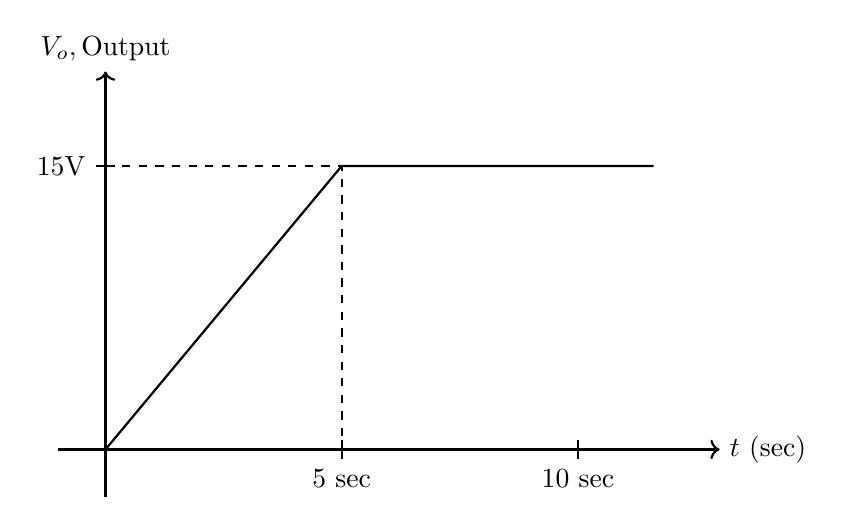
\begin{tikzpicture}[thick,scale=1.2]
        
        % ১. Axes (অক্ষসমূহ)
        \draw[->, thick] (-0.5, 0) -- (6.5, 0) node[right] {$t \text{ (sec)}$};
        \draw[->, thick] (0, -0.5) -- (0, 4) node[above] {$V_o, \text{Output}$};
        
        % ২. Y-axis Tick and Label (15V)
        % গ্রাফটি দেখতে সুন্দর করার জন্য 15V-কে y=3 পজিশনে ধরা হয়েছে
        \draw (0.1, 3) -- (-0.1, 3) node[left] {$15\mathrm{V}$};
        
        % ৩. X-axis Ticks and Labels (5 sec and 10 sec)
        % স্কেলিং ঠিক রাখার জন্য 5 sec-কে x=2.5 এবং 10 sec-কে x=5 পজিশনে ধরা হয়েছে
        \draw (2.5, 0.1) -- (2.5, -0.1) node[below] {$5 \text{ sec}$};
        \draw (5.0, 0.1) -- (5.0, -0.1) node[below] {$10 \text{ sec}$};
        
        % ৪. Dashed Guidelines (ড্যাশড লাইন)
        \draw[dashed] (0, 3) -- (2.5, 3) -- (2.5, 0);
        
        % ৫. The Main Graph Curve (মূল গ্রাফের রেখা)
        % রেখাটি (0,0) থেকে শুরু হয়ে (2.5, 3) তে উঠবে, এরপর সোজা ডানদিকে যাবে
        \draw[thick] (0, 0) -- (2.5, 3) -- (5.8, 3);
        
    \end{tikzpicture}
\end{center}
\mk{15} \yr{EEE 263 | L-2/T-1 | 2014--15}

\end{enumerate}

%%──────────────────────────────────────────────────────────────────────
\subtopic{cE}{Analog Computing (Differential Equations)}
\label{sub:s7-analog}

\begin{enumerate}\item Design a circuit using op-amps and other passive elements to solve:
\[
2\frac{d^2v}{dt^2} - 3\frac{dv}{dt} + 4v + 5 = 0
\]
Draw the overall connection diagram and specify element values. Assume op-amps biased with $\pm15\,\text{V}$; all initial conditions are zero.
\mk{17} \yr{EEE 263 | L-2/T-1 | 2024--25}

\item Using op-amps, design a circuit to solve the following differential equation where $x$ is input and $y$ is output:
\[
\frac{d^2y}{dt^2} - 2\frac{dy}{dt} + 2y = 8x
\]
\mk{20} \yr{EEE 263 | L-2/T-1 | 2022--23}

\item Design an electronic analog computer using op-amp to solve the following differential equation. Give a brief explanation of the operation of the designed computer.
\[
\frac{d^2v}{dt^2} + 4\frac{dv}{dt} + 5v - 5 = 0
\]
\mk{26} \yr{EEE 263 | L-2/T-1 | 2018--19}

\item Design an analog computer circuit to solve the following differential equation for $t>0$:
\[
\frac{d^2v}{dt^2} + 3\frac{dv}{dt} + 2v + 4\cos(10t) = 0
\]
with initial conditions $v(0)=2$, $v'(0)=0$. An oscillator is available to provide $\sin(10t)$ signal.
\mk{20} \yr{EEE 263 | L-2/T-1 | 2015--16}

\item Design a circuit using Op-Amps that can solve the following differential equation:
\[
3\frac{d^2x(t)}{dt^2} + 4x(t) = 0
\]
Point out the node that represents the solution $x(t)$. Specify all the values of resistors and capacitors used.
\mk{20} \yr{EEE 263 | L-2/T-1 | 2014--15}

\item Design a circuit using op-amp that can provide solution to the following equation:
\[
3\frac{d^2v}{dt^2} + K\frac{dv}{dt} - 3v + 8 = 0
\]
where $K$ = last digit of your student ID. Briefly discuss the operation of your designed circuit.
\mk{29} \yr{EEE 263 | L-2/T-1 | Jan--2021}

\end{enumerate}

%%──────────────────────────────────────────────────────────────────────
\subtopic{cE}{Multiplier Circuit Design}
\label{sub:s7-mult}

\begin{enumerate}\item Suppose you have two input voltages $X_1$ and $X_2$. Design a circuit using Op-Amps that gives output $V_o = 10X_1 X_2$. The diodes available maintain the characteristic equation $I_D = I_s e^{V_D/nV_T}$ where $I_s = 10^{-6}\,\text{A}$. Specify all the values of resistors used.
\mk{26} \yr{EEE 263 | L-2/T-1 | 2014--15}

\end{enumerate}

%%──────────────────────────────────────────────────────────────────────
\subtopic{cE}{Frequency Multiplier}
\label{sub:s7-freqmult}

\begin{enumerate}\item You have two supply voltage sources, $v_1 = \sin(100t)\,\text{V}$ and $v_2 = 1\,\text{V}$. Design a circuit using op-amps that will produce an output voltage $v_o = (\sin(50t))^2\,\text{V}$. Also show that this circuit produces this output.
\mk{20} \yr{EEE 263 | L-2/T-1 | 2021--22}

\item Suppose you have a sinusoidal input voltage $V_{in}(t) = \sin(4000\pi t)$ volt. Design a frequency multiplier circuit using Op-Amps that multiplies the frequency by a factor of 2 to produce $V_{out}(t) = \sin(8000\pi t)$ volt. Use resistors, capacitors, inductors, and diodes (having reverse saturation current $10^{-6}\,\text{A}$) if necessary. Show necessary calculations and specify all design parameter values.
\mk{26} \yr{EEE 263 | L-2/T-1 | 2015--16}

\end{enumerate}

%%──────────────────────────────────────────────────────────────────────
\subtopic{cE}{Active Filters}
\label{sub:s7-filters}

\begin{enumerate}\item Design a 2nd order bandpass filter with lower cutoff frequency $f_{CL}=20\,\text{kHz}$ and higher cutoff frequency $f_{CH}=200\,\text{kHz}$.
\mk{10} \yr{EEE 263 | L-2/T-1 | 2017--18}

\item Determine the type of filter shown in the circuit by computing the transfer function in the frequency domain.
\begin{center}
      \begin{circuitikz}[thick,scale=1.2, transform shape]
        % ==========================================
        % Main Op-Amp
        % ==========================================
        \draw (0,0) node[op amp] (opamp) {};
        
        % Grounding the non-inverting (+) input
        \draw (opamp.+) -- ++(0,-0.5) node[ground] {};
        
        % Output connection and label
        \draw (opamp.out) to[short] ++(1.5,0) node[right] {$V_{out}$};
        
        % Junction dot at inverting (-) input
        \node[circ] at (opamp.-) {};
        
        % ==========================================
        % Input Network (Series C1 and R1)
        % ==========================================
        % Defining coordinates for input nodes
        \draw (opamp.-) ++(-2.5,0) coordinate (mid_in);
        \draw (mid_in) ++(-2,0) coordinate (vin);
        
        % Drawing input components
        \draw (vin) node[left] {$V_{in}$} 
              to[R, l=$R_1$, o-]  (mid_in) 
              to[C, l=$C_1$] (opamp.-);
              
        % ==========================================
        % Feedback Network (Parallel R2 and C2)
        % ==========================================
        % Lower feedback branch (R2)
        \draw (opamp.-) -- ++(0,1.5) coordinate (fb_lower_left);
        \draw (fb_lower_left) to[C, l=$C_2$] (fb_lower_left -| opamp.out) coordinate (fb_lower_right);
        \draw (fb_lower_right) -- (opamp.out);
        
        % Upper feedback branch (C2)
        \draw (fb_lower_left) -- ++(0,1.5) coordinate (fb_upper_left);
        \draw (fb_upper_left) to[R, l=$R_2$] (fb_upper_left -| opamp.out) coordinate (fb_upper_right);
        \draw (fb_upper_right) -- (fb_lower_right);
        
    \end{circuitikz}
\end{center}
\mk{20} \yr{EEE 263 | L-2/T-1 | 2016--17, 2017--18}

\item For the filter circuit given, determine (i) its type and comment on its order; derive the transfer function and find the cutoff frequency. (ii) If $R=10\,\text{k}\Omega$ and $C=0.1\,\mu\text{F}$, would it be possible to pass a 100\,Hz signal through this filter without distortion? Justify your answer. Note that the first Op-Amp block performs summation of input and output signals.
\begin{center}
      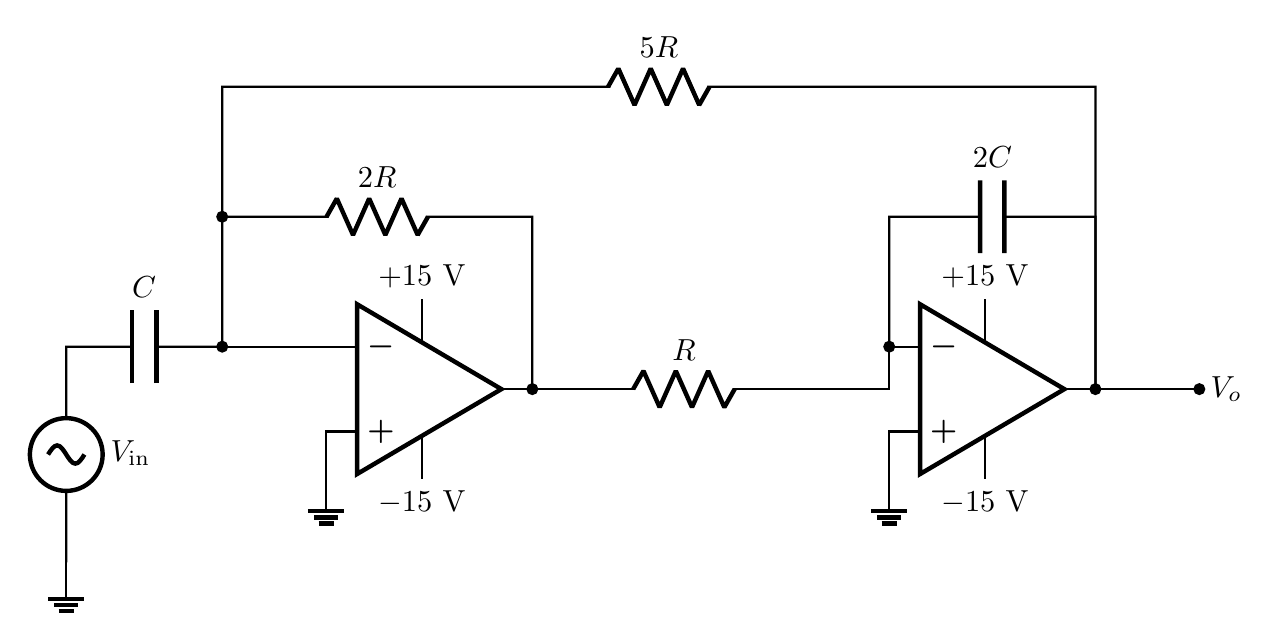
\begin{tikzpicture}[thick,scale=1.1, transform shape]
        
        % ==========================================
        % First Op-Amp Stage
        % ==========================================
        \node[op amp] (op1) at (0,0) {};
        
        % Power and Ground for Op-Amp 1
        \draw (op1.+) -- ++(0,-0.5) node[ground] {};
        \draw (op1.up) -- ++(0,0.5) node[above] {$+15\ \mathrm{V}$};
        \draw (op1.down) -- ++(0,-0.5) node[below] {$-15\ \mathrm{V}$};
        
        % ==========================================
        % Second Op-Amp Stage
        % ==========================================
        \node[op amp] (op2) at (6.5,0) {};
        
        % Power and Ground for Op-Amp 2
        \draw (op2.+) -- ++(0,-0.5) node[ground] {};
        \draw (op2.up) -- ++(0,0.5) node[above] {$+15\ \mathrm{V}$};
        \draw (op2.down) -- ++(0,-0.5) node[below] {$-15\ \mathrm{V}$};
        
        % ==========================================
        % Input Section (Vin and Capacitor C)
        % ==========================================
        % Junction node before Op-Amp 1
        \draw (op1.-) -- ++(-1.2,0) coordinate (in_node) node[circ] {};
        
        % Source and Capacitor C
        \draw (in_node) to[C, l_=$C$] ++(-1.8,0) coordinate (v_top) 
              to[sV, l=$V_{\mathrm{in}}$] (v_top |- 0,-2) node[ground] {};
              
        % ==========================================
        % Inter-stage Connection (Resistor R)
        % ==========================================
        % Connect Op-Amp 1 output to Op-Amp 2 inverting input
        \draw (op1.out) node[circ] {} -- ++(0.5,0) 
              to[R, l=$R$] ++(2.5,0) -| (op2.-) node[circ] {};
              
        % ==========================================
        % Feedback Loops
        % ==========================================
        % Feedback 1: 2R (Local for Op-Amp 1)
        \draw (in_node) -- ++(0, 1.5) coordinate (fb1) node[circ] {} 
              to[R, l=$2R$] (fb1 -| op1.out) -- (op1.out);
              
        % Feedback 2: 2C (Local for Op-Amp 2)
        \draw (op2.-) -- ++(0, 1.5) coordinate (fb2) 
              to[C, l=$2C$] (fb2 -| op2.out) -- (op2.out) node[circ] {};
              
        % Global Feedback: 5R (From output back to input)
        \draw (fb1) -- ++(0, 1.5) coordinate (gfb) 
              to[R, l=$5R$] (gfb -| op2.out) -- (op2.out);
              
        % ==========================================
        % Output Node
        % ==========================================
        \draw (op2.out) -- ++(1.2,0) node[right] {$V_o$} node[circ] {};
        
    \end{tikzpicture}
\end{center}
\mk{23} \yr{EEE 263 | L-2/T-1 | 2015--16}

\item In the circuit shown, input voltage is $v_{in}(t) = 5 + 3\cos(300\pi t - 30°) + 8\sin(1000\pi t) + 7\sin(1600\pi t + 45°)$ volt. Design the active filter blocks and summing amplifier to obtain output $V_{out}(t) = 7 + 12\sin(1000\pi t)$ volt. Sketch the frequency response and specify the cutoff frequency for each filter. Specify all values of resistors and capacitors/inductors.
\begin{center}
  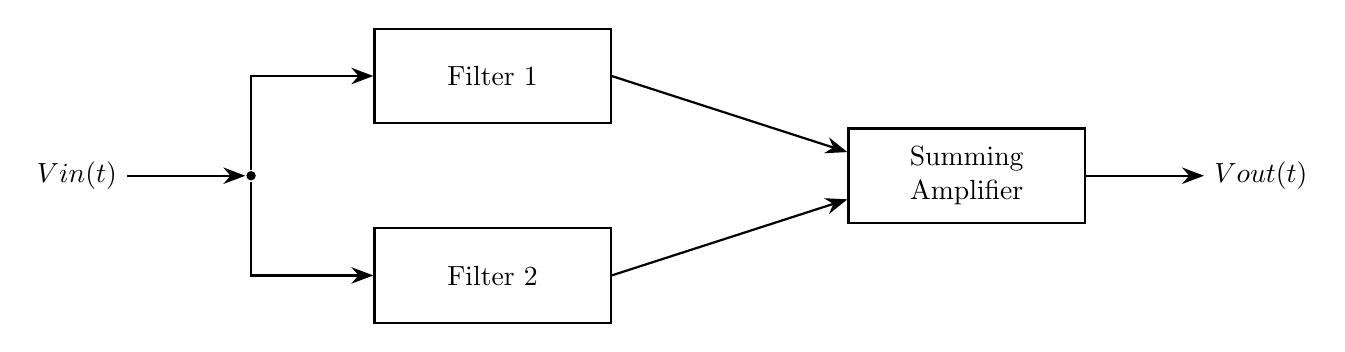
\begin{tikzpicture}[thick,
        % Style definitions
        block/.style={
            rectangle, 
            draw=black, 
            thick, 
            minimum width=3cm, 
            minimum height=1.2cm, 
            align=center,
            fill=white
        },
        arrow/.style={
            -{Stealth[scale=1.2]}, 
            thick
        }
    ]

        % ==========================================
        % Nodes / Blocks Placement
        % ==========================================
        % Central reference point for splitting the input
        \node (split) at (0,0) [circle, fill=black, inner sep=1.2pt] {};
        
        % Input label placed to the left of the split point
        \node (in_label) [left=1.5cm of split] {$Vin(t)$};
        
        % Filter blocks (Upper and Lower paths)
        \node (filter1) [block, above right=0.6cm and 1.5cm of split] {Filter 1};
        \node (filter2) [block, below right=0.6cm and 1.5cm of split] {Filter 2};
        
        % Summing Amplifier block placed downstream
        \node (sum) [block, right=7.5cm of split] {Summing\\Amplifier};
        
        % Output label
        \node (out_label) [right=1.5cm of sum] {$Vout(t)$};

        % ==========================================
        % Connections / Arrows
        % ==========================================
        % Main Input Arrow
        \draw [arrow] (in_label) -- (split);
        
        % Path to Filter 1 (Up and Right)
        \draw [arrow] (split) |- (filter1.west);
        
        % Path to Filter 2 (Down and Right)
        \draw [arrow] (split) |- (filter2.west);
        
        % Filter 1 output to Summing Amplifier
        \draw [arrow] (filter1.east) --([yshift=0.3cm]sum.west);
        
        % Filter 2 output to Summing Amplifier
        \draw [arrow] (filter2.east) -- ([yshift=-0.3cm]sum.west);
        
        % Final Output Arrow
        \draw [arrow] (sum.east) -- (out_label);

    \end{tikzpicture}
\end{center}
\mk{23} \yr{EEE 263 | L-2/T-1 | 2015--16}

\item Write the equation of magnitude of gain of a $-20\,\text{dB/decade}$ low pass filter. Why is it called a $-20\,\text{dB/decade}$ filter? Can it also be called a $-6\,\text{dB/octave}$ filter?
\mk{20} \yr{EEE 263 | L-2/T-1 | 2014--15}

\item Design a notch filter that eliminates any signal between 8\,kHz and 12\,kHz using op-amps. Specify all the values of resistors and capacitors used.
\mk{20} \yr{EEE 263 | L-2/T-1 | 2014--15}

\item A system blocks 20\,Hz and 20\,kHz but passes 10\,kHz. (i) Draw the frequency response of the system. (ii) Draw a block diagram of the system.
\mk{15} \yr{EEE 263 | L-2/T-1 | 2013--14}

\item Design a 40\,dB low pass filter (LPF) with a cutoff frequency of 1\,kHz. You have only one op-amp.
\mk{15} \yr{EEE 263 | L-2/T-1 | 2013--14}

\item Draw the circuit diagram of a $-20\,\text{dB/dec}$ low pass filter. Also write down the design procedure. Design a $-20\,\text{dB/dec}$ low pass filter with a cut-off frequency of 100\,kHz.
\mk{16} \yr{EEE 263 | L-2/T-1 | 2011--12}

\end{enumerate}

%%──────────────────────────────────────────────────────────────────────
\subtopic{cE}{Voltage-to-Current Converter}
\label{sub:s7-v2i}

\begin{enumerate}\item The circuit shown in Figure functions as a voltage-to-current converter. The op-amp used in this circuit is biased using $\pm 20\text{ V}$ sources. The overall circuit operates in the linear region as long as $V_{\text{out}}$ stays within the bias voltage range, and the concept of virtual short (i.e. $V_1 = V_2$) can be applied under such circumstances. If $V_{\text{out}}$ attempts to exceed these limits, the amplifier enters saturation, and the virtual short assumption becomes invalid. Given the circuit parameters $R_1 = R_2 = 10\text{ k}\Omega$, $R_3 = R_4 = 1\text{ k}\Omega$ and $R_{\text{L}} = 100\ \Omega$, calculate the load current $i_{\text{L}}$ and output voltage $V_{\text{out}}$ for and input voltage of $V_{\text{in}} = -5\text{ V}$.
\begin{center}
    
\begin{circuitikz}[american, line width=0.8pt]

    % --- Central Op-Amp ---
    % Positioned at (3, 0) to give plenty of room on all sides
    \node[op amp] (opamp) at (3, 0) {};
    
    % Power Supply Terminals (well-spaced from feedback paths)
    \draw (opamp.up) to[short, -o] ++(0, 0.6) node[above] {$V^+$};
    \draw (opamp.down) to[short, -o] ++(0, -0.6) node[below] {$V^-$};


    % --- Inverting (-) Input Path ---
    % Node V1 located at (-1, 0.5)
    \coordinate (V1) at (-1, 0.5);
    \fill (V1) circle (2pt) node[below left=3pt] {$V_1$};
    
    % Input wire with plenty of space for i^- current arrow
    \draw (V1) to[short, i^={$i^{-}= 0\text{ A}$}] (opamp.-);
    
    % Input Resistor R1 (Spanned across 3.5 units to prevent text crowding)
    \draw (-4.5, 0.5) node[left] {$V_{\text{in}}$} 
          to[short, o-] (-4.0, 0.5) 
          to[R, l={$R_1=10\text{ k}\Omega$}] (V1);


    % --- Feedback Loop (R2) ---
    % Lifted high up to y=3.0 to completely clear the Op-Amp and V+ label
    \draw (V1) -- (-1, 3.0) 
          to[R, l={$R_2=10\text{ k}\Omega$}] (6.0, 3.0) 
          -- (6.0, 0);


    % --- Output Section ---
    \draw (opamp.out) -- (6.0, 0);
    \fill (6.0, 0) circle (2pt);
    \draw (6.0, 0) to[short, -o] (7.5, 0) node[right] {$V_{\text{out}}$};


    % --- Non-Inverting (+) Input Path ---
    % Wire from '+' terminal extending left, then down to Node V2 at (-1, -3.0)
    \coordinate (V2) at (-1, -3.0);
    
    \draw (-1, -0.5) to[short, i^={$i^{+}= 0\text{ A}$}] (opamp.+);
    \draw (-1, -0.5) -- (V2);
    \fill (V2) circle (2pt) node[below left=3pt] {$V_2$};


    % --- Bottom Interconnection & Right Branches ---
    % Horizontal rail connecting V2 to the right-hand network
    \draw (V2) -- (6.0, -3.0);
    \fill (6.0, -3.0) circle (2pt);

    % R3 Branch (Dropped from output down to the middle rail)
    % Separated the resistor label, value, and current arrow vertically
    \draw (6.0, 0) to[R, l=$R_3$, label={$R_3=1\text{ k}\Omega$}] (6.0, -1.8)
          to[short, i=$i_3$] (6.0, -3.0);

    % R4 Ground Branch (Left side, below V2)
    \draw (V2) to[R, l=$R_4$, label={$R_4=1\text{ k}\Omega$}] (-1, -5.5) node[ground] {};

    % RL Load Branch (Right side, below middle rail)
    \draw (6.0, -3.0) to[R, l=$R_L$] (6.0, -4.6)
          to[short, i=$i_L$] (6.0, -5.5) node[ground] {};


\end{circuitikz}
\end{center}
\mk{18} \yr{EEE 263 | L-2/T-1 | 2024--25}

\end{enumerate}

\subtopic{cE}{System Design (Analog to Digital Interface)}

%%──────────────────────────────────────────────────────────────────────\n\subtopic{cE}{System Design (Analog to Digital Interface)}
\label{sub:s7-sysdesign}

\begin{enumerate}


\item Design a circuit using Op-Amp and Digital Circuits for given input wave shape $v_{\text{in}}$ and output wave shape $v_{\text{out}}$ in Figure . Assume a $5\text{ V}$ level to be digital 1 and $-5\text{ V}$ level to be digital 0.

\begin{center}
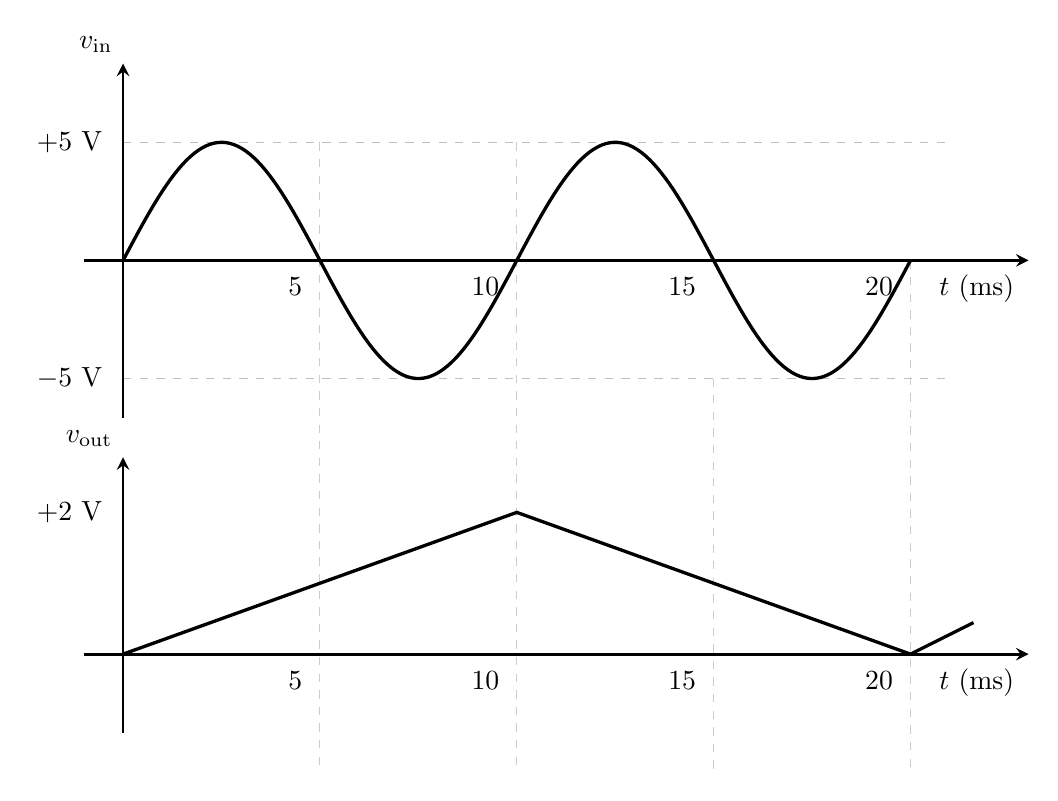
\begin{tikzpicture}[scale=1.0]

    % ==========================================
    % TOP GRAPH: Input Voltage (v_in)
    % ==========================================
    \begin{scope}[shift={(0,5)}]
        % Grid/Helper lines for alignment (Dashed)
        \draw[dashed, color=gray!50] (0, 1.5) -- (10.5, 1.5);
        \draw[dashed, color=gray!50] (0, -1.5) -- (10.5, -1.5);
        \draw[dashed, color=gray!40] (2.5, 1.5) -- (2.5, -6.5);   % t = 5 ms line
        \draw[dashed, color=gray!40] (5.0, 1.5) -- (5.0, -6.5);   % t = 10 ms line
        \draw[dashed, color=gray!40] (7.5, -1.5) -- (7.5, -6.5);  % t = 15 ms line
        \draw[dashed, color=gray!40] (10.0, 0) -- (10.0, -6.5);   % t = 20 ms line

        % Axes
        \draw[->, >=stealth, line width=1pt] (-0.5, 0) -- (11.5, 0) node[below left=2pt] {$t\text{ (ms)}$};
        \draw[->, >=stealth, line width=1pt] (0, -2.0) -- (0, 2.5) node[above left] {$v_{\text{in}}$};

        % Sine Wave Function Plots (Two complete cycles)
        % Period T = 10ms -> represented by 5 units on x-axis scale
        \draw[line width=1.2pt, color=black] plot[domain=0:10, samples=200] (\x, {1.5*sin(\x*72)});

        % Y-Axis Labels
        \node[left=4pt] at (0, 1.5) {$+5\text{ V}$};
        \node[left=4pt] at (0, -1.5) {$-5\text{ V}$};

        % X-Axis Time Markers
        \node[below left=4pt] at (2.5, 0) {$5$};
        \node[below left=4pt] at (5.0, 0) {$10$};
        \node[below left=4pt] at (7.5, 0) {$15$};
        \node[below left=4pt] at (10.0, 0) {$20$};
    \end{scope}


    % ==========================================
    % BOTTOM GRAPH: Output Voltage (v_out)
    % ==========================================
    \begin{scope}[shift={(0,0)}]
        % Axes
        \draw[->, >=stealth, line width=1pt] (-0.5, 0) -- (11.5, 0) node[below left=2pt] {$t\text{ (ms)}$};
        \draw[->, >=stealth, line width=1pt] (0, -1.0) -- (0, 2.5) node[above left] {$v_{\text{out}}$};

        % Triangular Wave Output Plot
        % Rises linearly to 2V at t=10ms, drops to 0V at t=20ms, then starts rising again
        \draw[line width=1.2pt, color=black] (0,0) -- (5.0, 1.8) -- (10.0, 0) -- (10.8, 0.4);

        % Y-Axis Label
        \node[left=4pt] at (0, 1.8) {$+2\text{ V}$};

        % X-Axis Time Markers
        \node[below left=4pt] at (2.5, 0) {$5$};
        \node[below left=4pt] at (5.0, 0) {$10$};
        \node[below left=4pt] at (7.5, 0) {$15$};
        \node[below left=4pt] at (10.0, 0) {$20$};
    \end{scope}

\end{tikzpicture}
    
\end{center}

\mk{26.67} \yr{EEE 263 | L-2/T-1 | 2017--18}

\item A circuit is to be designed where depending on the range of input voltage a digital sequence is passed to a computer. The ranges and corresponding digital sequences are:
\begin{center}
\begin{tabular}{ll}
\toprule
\textbf{Range} & \textbf{Digital Sequence} \\
\midrule
0 -- 1.2\,V & 010 \\
1.2 -- 3.2\,V & 110 \\
3.2 -- 3.5\,V & 001 \\
3.5 -- 5\,V & 111 \\
\bottomrule
\end{tabular}
\end{center}
Design a circuit using op-amps and digital circuits (gates, multiplexers) to perform the task. Assume 5\,V = digital 1 and 0\,V = digital 0.
\mk{25} \yr{EEE 263 | L-2/T-1 | 2016--17}

\end{enumerate}

%%──────────────────────────────────────────────────────────────────────
\subtopic{cE}{Waveform Realization}
\label{sub:s7-wavereal}

\begin{enumerate}\item Determine an op-amp circuit realization for given input wave shapes $V_1$ and $V_2$ and output wave shape $V_{out}$.
\begin{center}
  
    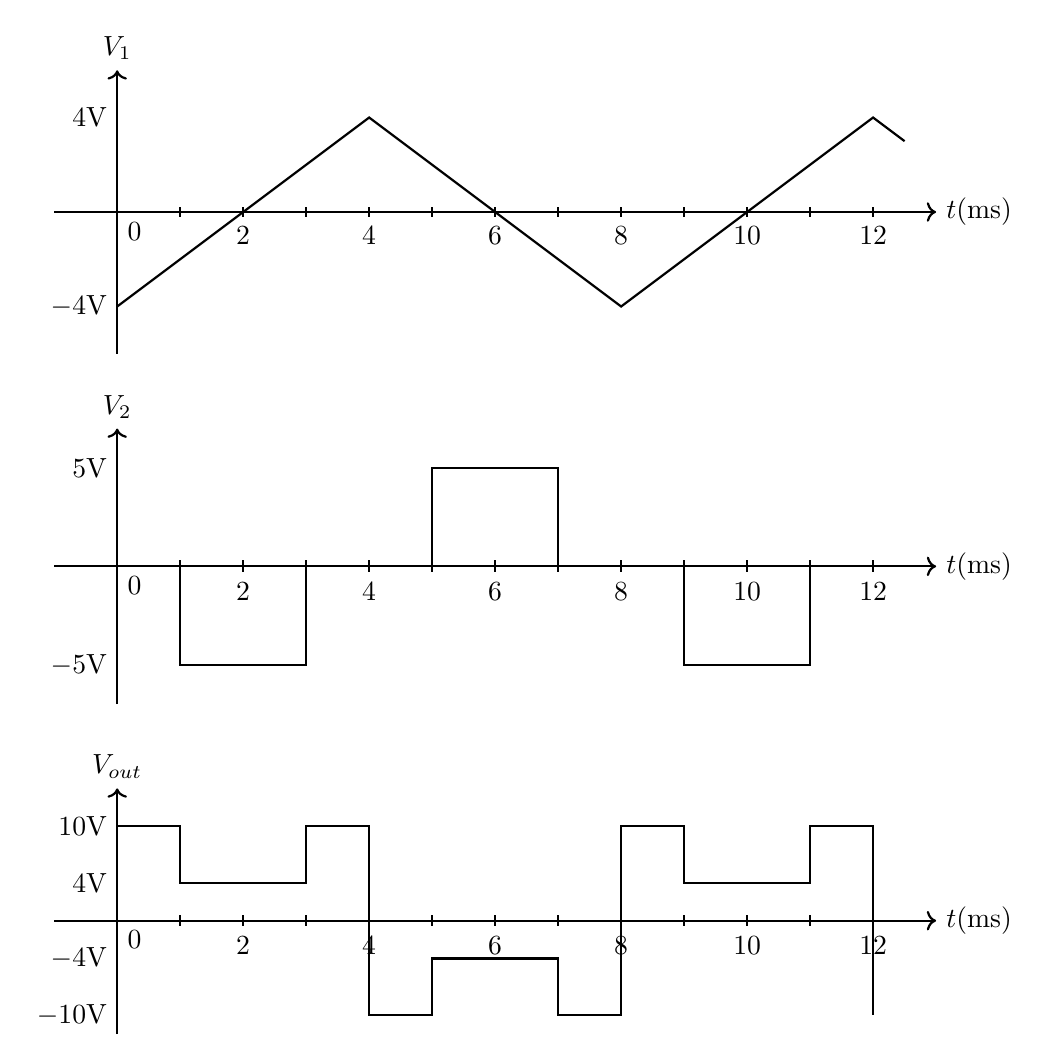
\begin{tikzpicture}[thick,x=0.8cm]
        
        % ==========================================
        % V1 Graph (Top)
        % ==========================================
        \begin{scope}[yshift=9cm, y=0.3cm]
            % Axes
            \draw[->, thick] (-1, 0) -- (13, 0) node[right] {$t$(ms)};
            \draw[->, thick] (0, -6) -- (0, 6) node[above] {$V_1$};
            
            % X-axis ticks and labels
            \foreach \x in {1,2,...,12} {
                \draw (\x, 0.2) -- (\x, -0.2);
            }
            \foreach \x in {2,4,6,8,10,12} {
                \node[below] at (\x, -0.2) {\x};
            }
            \node[below right] at (0, 0) {0};
            
            % Y-axis labels
            \node[left] at (0, 4) {$4$V};
            \node[left] at (0, -4) {$-4$V};
            
            % Waveform (Triangle Wave)
            \draw[thick] (0,-4) -- (4,4) -- (8,-4) -- (12,4) -- (12.5, 3);
        \end{scope}

        % ==========================================
        % V2 Graph (Middle)
        % ==========================================
        \begin{scope}[yshift=4.5cm, y=0.25cm]
            % Axes
            \draw[->, thick] (-1, 0) -- (13, 0) node[right] {$t$(ms)};
            \draw[->, thick] (0, -7) -- (0, 7) node[above] {$V_2$};
            
            % X-axis ticks and labels
            \foreach \x in {1,2,...,12} {
                \draw (\x, 0.3) -- (\x, -0.3);
            }
            \foreach \x in {2,4,6,8,10,12} {
                \node[below] at (\x, -0.3) {\x};
            }
            \node[below right] at (0, 0) {0};
            
            % Y-axis labels
            \node[left] at (0, 5) {$5$V};
            \node[left] at (0, -5) {$-5$V};
            
            % Waveform (Pulse Wave)
            \draw[thick] (0,0) -- (1,0) -- (1,-5) -- (3,-5) -- (3,0) 
                      -- (5,0) -- (5,5) -- (7,5) -- (7,0) 
                      -- (9,0) -- (9,-5) -- (11,-5) -- (11,0) -- (12.5,0);
        \end{scope}

        % ==========================================
        % Vout Graph (Bottom)
        % ==========================================
        \begin{scope}[yshift=0cm, y=0.12cm]
            % Axes
            \draw[->, thick] (-1, 0) -- (13, 0) node[right] {$t$(ms)};
            \draw[->, thick] (0, -12) -- (0, 14) node[above] {$V_{out}$};
            
            % X-axis ticks and labels
            \foreach \x in {1,2,...,12} {
                \draw (\x, 0.6) -- (\x, -0.6);
            }
            \foreach \x in {2,4,6,8,10,12} {
                \node[below] at (\x, -0.6) {\x};
            }
            \node[below right] at (0, 0) {0};
            
            % Y-axis labels
            \node[left] at (0, 10) {$10$V};
            \node[left] at (0, 4) {$4$V};
            \node[left] at (0, -4) {$-4$V};
            \node[left] at (0, -10) {$-10$V};
            
            % Waveform (Multi-level Output)
            \draw[thick] (0,10) -- (1,10) -- (1,4) -- (3,4) -- (3,10) -- (4,10) 
                      -- (4,-10) -- (5,-10) -- (5,-4) -- (7,-4) -- (7,-10) 
                      -- (8,-10) -- (8,10) -- (9,10) -- (9,4) -- (11,4) 
                      -- (11,10) -- (12,10) -- (12,-10);
        \end{scope}


    \end{tikzpicture}
\end{center}
\mk{15} \yr{EEE 263 | L-2/T-1 | 2016--17}

\end{enumerate}

%%──────────────────────────────────────────────────────────────────────
\subtopic{cE}{Integrator}
\label{sub:s7-integrator}

\begin{enumerate}
    
\item Design a circuit using ideal operational amplifiers that implements the following equation:
\[
v_0 \propto \int (v_1 + v_2)\,dt
\]
Write the final output expression in terms of the circuit components used in your design.
\mk{20} \yr{EEE 263 | L-2/T-1 | 2020--21}

\item The input voltage $v_I$ and output voltage $v_O$ of an op-amp based circuit are given. Design the circuit. 
\begin{center}
    \begin{tikzpicture}[thick,>=latex]

    \draw[->] (-1,0) -- (6,0) node[right] {$t$};
    \draw[->] (0,-0.5) -- (0,2.5) node[above] {$v_I(t)$};
    
    % Waveform (Cyan color, very thick)
    \draw[cyan, very thick] (-0.5,0) -- (0,0) -- (0,1.5) -- (3,1.5) -- (3,0) -- (5,0);
    
    % Labels & Ticks
    \node[below left] at (0,0) {0};
    \node[left] at (0,1.5) {1 V};
    \node[below] at (3,0) {1 ms};
    
    % Caption
    \node[below] at (2.5,-0.8) {(a)};
\end{tikzpicture}

     \begin{tikzpicture}[thick,>=latex]

    % Axes
    \draw[->] (-1,0) -- (6,0) node[right] {$t$};
    \draw[->] (0,-3) -- (0,1.5) node[above] {$v_O(t)$};
    
    % Waveform (Cyan color, very thick)
    \draw[cyan, very thick] (-0.5,0) -- (0,0) -- (3,-2) -- (5,-2);
    
    % Dashed alignment lines
    \draw[dashed] (3,0) -- (3,-2);
    \draw[dashed] (0,-2) -- (3,-2);
    
    % Labels & Ticks
    \node[below left] at (0,0) {0};
    \node[left] at (0,-2) {$-10$ V};
    \node[below right] at (3,0) {1 ms};
    
    % Caption
    \node[below] at (2.5,-3.2) {(b)};

\end{tikzpicture}
\end{center}
\mk{17} \yr{EEE 263 | L-2/T-1 | Jan--2021}

\end{enumerate}

%%──────────────────────────────────────────────────────────────────────
\subtopic{cE}{Op-Amp Network Analysis}
\label{sub:s7-network}

\begin{enumerate}\item Determine the closed-loop voltage gain and current gain of the ideal op-amp network shown in the figure.
\begin{center}
    
\begin{circuitikz}[thick,american, thick]

    % --- Operational Amplifier ---
    \node[op amp] (opamp) at (0,0) {};

    % --- Inverting Input (-) Network ---
    % Create a junction node further to the left to widen the feedback loop
    \coordinate (in_node) at ($(opamp.-) + (-2,0)$);
    \draw (opamp.-) -- (in_node);
    \filldraw (in_node) circle (1.5pt);

    % Input Resistor R1 and Input Terminal v_I
    \draw ($(in_node) + (-2.5,0)$) node[left] {$v_I$} to[short, o-] ($(in_node) + (-2,0)$)
          to[R, l=$R_1$] (in_node);

    % --- Non-inverting Input (+) Network ---
    % Connected to ground
    \draw (opamp.+) -- ++(-0.5,0) -- ++(0,-0.5) node[ground] {};

    % --- Output Network ---
    % Create a junction node further to the right to widen the feedback loop
    \coordinate (out_node) at ($(opamp.out) + (2,0)$);
    \draw (opamp.out) -- (out_node);
    \filldraw (out_node) circle (1.5pt); 
    
    % Output terminal v_O
    \draw (out_node) to[short, -o] ++(1,0) node[right] {$v_O$};

    % --- Feedback T-Network ---
    % Raised to y=3.5 so R4 and its ground don't overlap with the op-amp body
    \coordinate (fb_left) at (in_node |- 0, 3.5);
    \coordinate (fb_right) at (out_node |- 0, 3.5);
    \coordinate (fb_mid) at (0, 3.5);
    
    \draw (in_node) -- (fb_left);
    \draw (out_node) -- (fb_right);
    
    % Midpoint for the T-junction
    \filldraw (fb_mid) circle (1.5pt);
    
    % Resistors R2 and R3 (now with enough horizontal space)
    \draw (fb_left) to[R, l_=$R_2$] (fb_mid);
    \draw (fb_mid) to[R, l_=$R_3$] (fb_right);
    
    % Resistor R4 to ground, dropping down but stopping at y=1.5 (above the op-amp)
    \draw (fb_mid) to[R, l=$R_4$] (0, 1.5) node[ground] {};

\end{circuitikz}
\end{center}
\mk{23} \yr{EEE 263 | L-2/T-1 | 2020--21}

\item Determine the differential equation solved by the circuit shown: (i) when the capacitor $C$ is absent; (ii) when the capacitor $C$ is present. At what value of $C$ does the circuit become a non-inverting amplifier?
\begin{center}
      \begin{circuitikz}[thick,scale=1.2, transform shape]
        % ==========================================
        % Main Op-Amp
        % ==========================================
        \draw (0,0) node[op amp] (opamp) {};
        
        % Output node and label Vout
        \draw (opamp.out) -- ++(1.5,0) coordinate (out_node);
        \node[circ] at (out_node) {};
        \node[right] at (out_node) {$V_{out}$};
        
        % ==========================================
        % Inverting Input (-) Network (Top side)
        % ==========================================
        \draw (opamp.-) -- ++(-0.5,0) coordinate (neg_node);
        \node[circ] at (neg_node) {};
        
        % R1 to ground
        \draw (neg_node) ++(-2.5,0) coordinate (r1_end) 
              to[R, l=$R_1$] (neg_node);
        \draw (r1_end) -- ++(0,0) node[ground] {};
        
        % R2 Feedback Loop
        \draw (neg_node) -- ++(0, 1.5) coordinate (top_fb)
              to[R, l=$R_2$] (top_fb -| out_node)
              -- (out_node);

        % ==========================================
        % Non-Inverting Input (+) Network (Bottom side)
        % ==========================================
        \draw (opamp.+) -- ++(-0.5,0) coordinate (pos_node);
        \node[circ] at (pos_node) {};
        
        % Vin and Rin
        \draw (pos_node) ++(-2.5,0) coordinate (vin_node);
        \node[ocirc] at (vin_node) {};
        \node[left] at (vin_node) {$V_{in}$};
        \draw (vin_node) to[R, l=$R_{in}$] (pos_node);
        
        % Node connection for C and Cin split
        \draw (pos_node) -- ++(0, -1.2) coordinate (c_mid);
        \node[circ] at (c_mid) {};
        
        % Cin to ground
        \draw (c_mid) to[C, l=$C_{in}$] ++(0, -1.5) node[ground] {};
        
        % C feedback from output
        \draw (c_mid) to[C, l=$C$] (c_mid -| out_node) -- (out_node);
        
    \end{circuitikz}
\end{center}
\mk{21} \yr{EEE 263 | L-2/T-1 | 2016--17}

\item Determine the Boolean expression for $V_0$ in terms of the four input voltages for the circuit shown (diode logic).
\begin{center}
  
    % Scale kept to 1.0 so it respects standard page margins perfectly
    \begin{circuitikz}[thick,x=1.2cm, transform shape]
        % Slightly scaling down the component symbols keeps the wire paths looking spacious
        \ctikzset{resistors/scale=0.8, diodes/scale=0.8}

        % ==========================================
        % Inputs V1, V2 and Top AND Gate (D1, D2, R1)
        % ==========================================
        \draw (0, 9) node[left] {$V_1$} to[short, o-] (0.5, 9);
        \draw (0, 7) node[left] {$V_2$} to[short, o-] (0.5, 7);
        
        % Diodes D1, D2 (Cathodes at the inputs)
        \draw (2.5, 9) to[D, l=$D_1$] (0.5, 9);
        \draw (2.5, 7) to[D, l=$D_2$] (0.5, 7);
        \draw (2.5, 9) -- (2.5, 7);
        
        % Node A and Pull-up R1
        \node[circ] (NodeA) at (2.5, 8) {};
        \draw (2.5,9) to[R, l=$R_1$, a=$1\text{ k}\Omega$] (2.5, 10.5) node[vcc] {$+5\text{V}$};

        % ==========================================
        % Inputs V3, V4 and Bottom AND Gate (D5, D6, R3)
        % ==========================================
        \draw (0, 4) node[left] {$V_3$} to[short, o-] (0.5, 4);
        \draw (0, 2) node[left] {$V_4$} to[short, o-] (0.5, 2);
        
        % Diodes D5, D6
        \draw (2.5, 4) to[D, l=$D_5$] (0.5, 4);
        \draw (2.5, 2) to[D, l=$D_6$] (0.5, 2);
        \draw (2.5, 4) -- (2.5, 2);
        
        % Node B and Pull-up R3
        \node[circ] (NodeB) at (2.5, 3) {};
        \draw (3.5,3) to[R, l=$R_3$, a=$1\text{ k}\Omega$, *-] (3.5, 5.5) node[vcc] {$+5\text{V}$};

        % ==========================================
        % Level Shift / Coupling (D3, Node C, R2, D4)
        % ==========================================
        \draw (NodeA) to[D, l=$D_3$] (5, 8) coordinate (NodeC);
        \node[circ] at (NodeC) {};

        % Pull-up R2
        \draw (NodeC) to[R, l={$R_2=1\text{ k}\Omega$}, *-] (5, 10.5) node[vcc] {$+5\text{V}$};
        
        % D4 Clamping Diode (Spaced safely to the right at X=6.5)
        \draw (NodeC) to[short, -*] (6.5, 8) coordinate (D4Junct);
        \draw (D4Junct) to[D, l=$D_4$] (6.5, 10.5) node[vcc] {$+5\text{V}$};

        % ==========================================
        % OR Gate Stage (D7, D8, Node E, R4)
        % ==========================================
        % Route from Top Branch
        \draw (D4Junct) -- (7.5, 8) -- (7.5, 6.5);
        \draw (7.5, 6.5) to[D, l=$D_7$] (9.5, 6.5);

        % Route from Bottom Branch (Node B)
        \draw (NodeB) -- (7.5, 3) -- (7.5, 4.5);
        \draw (7.5, 4.5) to[D, l=$D_8$] (9.5, 4.5);

        % Junction Node E
        \draw (9.5, 6.5) -- (9.5, 4.5);
        \node[circ] (NodeE) at (9.5, 5.5) {};

        % Pull-down R4
        \draw (10,5.5) to[R, l=$R_4$, a=$1\text{ k}\Omega$, *-] (10, 3) node[ground] {};

        % ==========================================
        % Output Stage (D9, Node F, D10, R5)
        % ==========================================
        \draw (NodeE) to[D, l=$D_9$] (12.5, 5.5) coordinate (NodeF);
        \node at (NodeF) {};

        % D10 Clamping Diode (Anode at ground, isolated vertically at X=11.5)
        \draw (12.5, 3) node[ground] {} to[D, l=$D_{10}$] (12.5,5.5);

        % Pull-down R5 (Safely shifted to X=13)
        \draw (NodeF) -- (13, 5.5) coordinate (VoutJunct);
        \node at (VoutJunct) {};
        \draw (14,5.5) to[R, l={$R_5=1\text{ k}\Omega$}] (14, 3) node[ground] {};

        % Final Output Vo
        \draw (VoutJunct) to[short, -o] (15, 5.5) node[right] {\Large $V_o$};

        % ==========================================
        % Figure Caption
        % ==========================================

    \end{circuitikz}

\end{center}
\mk{10} \yr{EEE 263 | L-2/T-1 | 2016--17}

\end{enumerate}

%%──────────────────────────────────────────────────────────────────────
\subtopic{cE}{Op-Amp Practical Imperfections}
\label{sub:s7-imperfections}

\begin{enumerate}\item What are the AC imperfections of a practical op-amp? How can we find out the value of input offset voltage and input offset current?
\mk{15} \yr{EEE 263 | L-2/T-1 | 2013--14}

\end{enumerate}

%%──────────────────────────────────────────────────────────────────────
\subtopic{cE}{Dual Slope A/D Converter}
\label{sub:s7-adc}

\begin{enumerate}\item By drawing appropriate circuits, explain the operation of a dual slope A/D converter.
\mk{20} \yr{EEE 263 | L-2/T-1 | 2020--21}

\end{enumerate}


%% ══════════════════════════════════════════════════════════════════════
%%  PART V
%% ══════════════════════════════════════════════════════════════════════
\secdivider{Part V --- Oscillators \& Timers}{Colpitts oscillator, 555 Timer astable design, triangular wave generators}{cF}

%% ══════════════════════════════════════════════════════════════════════
%%  SECTION 8: OSCILLATORS, TIMERS & FUNCTION GENERATORS
%% ══════════════════════════════════════════════════════════════════════
\markboth{S8: Oscillators \& Timers}{S8: Oscillators \& Timers}
\label{sec:S8}
\titleformat{\section}{\large\bfseries\color{cF}}{}{0em}{}[\titlerule]
\section*{S8 \quad Oscillators, Timers \& Function Generators}
\addcontentsline{toc}{section}{S8: Oscillators, Timers \& Function Generators}

%%──────────────────────────────────────────────────────────────────────
\subtopic{cF}{Barkhausen Stability Criterion}
\label{sub:s8-barkhausen}

\begin{enumerate}\item Write down the Barkhausen criterion.
\mk{10} \yr{EEE 263 | L-2/T-1 | 2018--19}

\item Derive expression of Desensitivity. Explain positive and negative feedback from desensitivity.
\mk{10+5} \yr{EEE 263 | L-2/T-1 | 2014--15}


\item Write down the Barkhausen stability criterion for an oscillation in a linear electronic circuit to sustain.
\mk{6} \yr{EEE 263 | L-2/T-1 | 2014--15}

\end{enumerate}

%%──────────────────────────────────────────────────────────────────────
\subtopic{cF}{Wien Bridge Oscillator}
\label{sub:s8-wien}



\begin{enumerate}

\item Define Barkhausen criterion. Describe the operating principle of an op-amp based Wein bridge oscillator. Derive the conditions for Barkhausen criteria to be satisfied in this oscillator and the expression of oscillation frequency.
\mk{17} \yr{EEE 263 | L-2/T-1 | 2023--24}    
   
\item For the Wien bridge circuit connected to an op-amp shown: 
\begin{enumerate}
    
\item  state conditions for sinusoidal oscillation;
\item derive the equation for oscillation frequency;
\item show that the voltage gain $A_V$ must be $\ge \left(1 + \frac{R_1}{R_2} + \frac{C_1}{C_2}\right)$ for oscillation to sustain; 
\item  if $R_1=R_2=10\,\text{k}\Omega$ and $C_1=C_2=0.1\,\mu\text{F}$, design the values of $R_3$ and $R_4$ so that oscillation sustains.
\end{enumerate}

 \begin{center}
    \begin{circuitikz}[thick,american, thick]

    % --- Wien Bridge Network ---
    % Define Bridge Nodes
    \coordinate (NT) at (0, 3);
    \coordinate (NB) at (0, -3);
    \coordinate (NL) at (-3, 0);
    \coordinate (NR) at (3, 0);

    % Top-Left Arm: Series C1, R1
    \draw (NT) to[C, l_=$C_1$] (-1.5, 1.5) to[R, l_=$R_1$] (NL);

    % Top-Right Arm: Resistor R3
    \draw (NT) to[R, l=$R_3$] (NR);

    % Bottom-Right Arm: Resistor R4
    \draw (NR) to[R, l=$R_4$] (NB);

    % Bottom-Left Arm: Parallel R2, C2
    % Inner path for R2
    \draw (NL) -- (-2, 0) to[R, l_=$R_2$] (0, -2) -- (NB);
    % Outer path for C2
    \draw (NL) -- (-3, -1) to[C, l_=$C_2$] (-1, -3) -- (NB);

    % Ground connection at bottom node
    \draw (NB) -- ++(0, -0.5) node[ground] {};

    % --- Operational Amplifier ---
    % Positioned to the right of the bridge
    \node[op amp, noinv input up] (opamp) at (7, 4) {};

    % Power Supply Terminals
    \draw (opamp.up) -- ++(0, 0.4) coordinate (vcc);
    \filldraw (vcc) circle (1.5pt) node[above] {+V};
    
    \draw (opamp.down) -- ++(0, -0.4) coordinate (vee);
    \filldraw (vee) circle (1.5pt) node[below] {-V};

    % --- Routing & Feedback Connections ---
    % Output Terminal and Feedback branching dot
    \coordinate (out_dot) at (8.5, 4);
    \draw (opamp.out) -- (out_dot);
    \filldraw (out_dot) circle (1.5pt);
    \draw (out_dot) to[short, -o] (10, 4) node[right] {V$_0$};

    % Output feedback to Top Node (NT)
    % Traced UP, then LEFT across the top of the circuit, then DOWN to NT
    \draw (out_dot) -- (8.5, 5.5) -- (0, 5.5) -- (NT);

    % Non-inverting Input (+) feedback to Left Node (NL)
    % Traced horizontally LEFT, then vertically DOWN to NL
    \draw (opamp.+) -| (NL);

    % Inverting Input (-) feedback to Right Node (NR)
    % Traced horizontally LEFT, then vertically DOWN to NR
    \draw (opamp.-) -| (NR);

    % --- Junction Dots ---
    \filldraw (NT) circle (1.5pt);
    \filldraw (NB) circle (1.5pt);
    \filldraw (NL) circle (1.5pt);
    \filldraw (NR) circle (1.5pt);

\end{circuitikz}
\end{center}
\mk{28} \yr{EEE 263 | L-2/T-1 | Jan--2021}    
    
    
\item Design a Wien Bridge Oscillator with an oscillation frequency of 1\,kHz. What is the gain of the feedback network of your design? Specify all the values of resistors and capacitors used.
\mk{20} \yr{EEE 263 | L-2/T-1 | 2014--15}

\item Design a Wien Bridge Oscillator with an oscillation frequency of 1000\,rad/sec. Available capacitors are 0.1\,$\mu$F, 1\,$\mu$F, and 100\,pF.
\mk{Unspecified} \yr{EEE 263 | L-2/T-1 | 2013--14}

\item Draw a Wien Bridge oscillator circuit and describe its operating principle.
\mk{17} \yr{EEE 263 | L-2/T-1 | 2012--13}


\end{enumerate}

%%──────────────────────────────────────────────────────────────────────
\subtopic{cF}{RC Phase Shift Oscillator}
\label{sub:s8-rcphase}

\begin{enumerate}
    
\item For an RC phase shift oscillator, derive the expression for oscillation frequency. Also derive the conditions for the Barkhausen criterion to be satisfied. Assume all resistors in the feedback network are of the same value and all capacitors are of the same value.
\mk{26} \yr{EEE 263 | L-2/T-1 | 2021--22}

\item For the oscillator circuit shown below,  find oscillation frequency ($\text{w}$), $\beta$-network gain ($\beta$), and amplifier gain ($\text{A}$). Also design this oscillator for an oscillation frequency of $1\text{ kHz}$.Note that, each state is separated by a source follower circuit. Hence each stage will give a phase shift of $60^\circ$ and 3 stages will give in total 180 phase shift. Here, $\beta = \frac{v_2}{v_1}$.

\begin{center}
    \begin{circuitikz}[american, line width=0.8pt]
    
        % =========================================================================
        % STAGE 1: Inverting Op-Amp with Feedback Resistor Rf and Output Node V1
        % =========================================================================
        % Position Op-Amp 1
        \node[op amp] (opamp1) at (3, 0) {};
        \node at (5, -2) {Stage 1};
        
        % Power Supply Terminals for Op-Amp 1
        \draw (opamp1.up) -- ++(0,0.2) node[above] {$+V$};
        \draw (opamp1.down) -- ++(0,-0.2) node[below] {$-V$};
        
        % Non-inverting input (+) to Ground
        \draw (opamp1.+) -- ++(-0.1,0) node[ground] {};
        
        % Inverting input (-) feedback junction
        \draw (opamp1.-) -- ++(-0.5,0) coordinate (FB1);
        
        % Feedback Loop with Rf
        \draw (FB1) -- ++(0, 1.8) coordinate (Rf_top_left)
              to[R, l=$R_f$] ++(3, 0) coordinate (Rf_top_right)
              -- (opamp1.out |- Rf_top_right) -- (opamp1.out);
              
        % Output node V1
        \fill (opamp1.out) circle (2pt) node[below right=2pt] {$V_1$};
    
    
        % =========================================================================
        % STAGE 2: Op-Amp Buffer/Amplifier with RC Network
        % =========================================================================
        % First High-Pass C-R Network connecting Stage 1 to Stage 2
        \draw (opamp1.out) to[C, l=$C$] ++(2.5, 0) coordinate (C1_out);
        \fill (C1_out) circle (2pt);
        \draw (C1_out) to[R, l_=$R$] ++(0, -2.2) node[ground] {};
        
        % Position Op-Amp 2 (shifted further right)
        \node[op amp] (opamp2) at (8.5, 0) {};
        \node at (10.5,-2) {Stage 2};
        
        % Power Supply Terminals for Op-Amp 2
        \draw (opamp2.up) -- ++(0,0.2) node[above] {$+V$};
        \draw (opamp2.down) -- ++(0,-0.2) node[below] {$-V$};
        
        % Non-inverting input (+) to Ground
        \draw (opamp2.+) -- ++(-0.2,0) node[ground] {};
        
        % Connection to Inverting Input (-) and Voltage Follower Feedback
        \draw (C1_out) -- (opamp2.-);
        \fill (opamp2.-) circle (2pt) coordinate (FB2);
        \draw (FB2) -- ++(0, 1.2) coordinate (top_left2)
              -- (opamp2.out |- top_left2) -- (opamp2.out);
              
        \fill (opamp2.out) circle (2pt);
    
    
        % =========================================================================
        % STAGE 3: Op-Amp Buffer/Amplifier with RC Network and Output Node V2
        % =========================================================================
        % Second High-Pass C-R Network connecting Stage 2 to Stage 3
        \draw (opamp2.out) to[C, l=$C$] ++(2.5, 0) coordinate (C2_out);
        \fill (C2_out) circle (2pt);
        \draw (C2_out) to[R, l_=$R$] ++(0, -2.2) node[ground] {};
        
        % Position Op-Amp 3 (shifted further right)
        \node[op amp] (opamp3) at (14.0, 0) {};
        \node at (16, -2) {Stage 3};
        
        % Power Supply Terminals for Op-Amp 3
        \draw (opamp3.up) -- ++(0,0.2) node[above] {$+V$};
        \draw (opamp3.down) -- ++(0,-0.2) node[below] {$-V$};
        
        % Non-inverting input (+) to Ground
        \draw (opamp3.+) -- ++(-0.2,0) node[ground] {};
        
        % Connection to Inverting Input (-) and Voltage Follower Feedback
        \draw (C2_out) -- (opamp3.-);
        \fill (opamp3.-) circle (2pt) coordinate (FB3);
        \draw (FB3) -- ++(0, 1.2) coordinate (top_left3)
              -- (opamp3.out |- top_left3) -- (opamp3.out);
    
    
        % =========================================================================
        % OUTPUT SECTION & LONG FEEDBACK LOOP back to Stage 1
        % =========================================================================
        % Third C-R Network at the output of Stage 3 leading to V2
        \draw (opamp3.out) to[C, l=$C$] ++(2.2, 0) coordinate (V2_node);
        \fill (V2_node) circle (2pt) node[above right] {$V_2$};
        
        \draw (V2_node) to[R, l=$R$] ++(0, -2.2) coordinate (R3_bottom);
        \fill (R3_bottom) circle (2pt);
    
        % Long Feedback wire returning from V2 (bottom of R3) all the way back to Stage 1 input
        \draw (R3_bottom) -- ++(0, -1.2) coordinate (FB_loop_bottom)
                          -- (FB1 |- FB_loop_bottom) 
                          -- (FB1);
    
    
        % =========================================================================
        % GLOBAL CAPTION
        % =========================================================================
    
    \end{circuitikz}
\end{center}

\mk{18} \yr{EEE 263 | L-2/T-1 | 2017--18}


\item For the RC phase shift oscillator shown:
\begin{enumerate}
  \item Determine the oscillation frequency $f_0$ and obtain the relationship between $R_i$ and $R_f$ for sustainable oscillation.
  \item How can you generate a 100\,kHz signal from this oscillator?
\end{enumerate}
\begin{center}
    \begin{circuitikz}[thick, american]
        \node[op amp] (O1) at (0,0) {};
        \node[op amp] (O2) at (-4.5,-0.5){};
        \draw (O2.out) to[R, l=$R$] (O1.+);
        \node[op amp] (O3) at (-9,-1){};
        \draw (O3.out) to[R, l=$R$] (O2.+);
        \draw(O3.-) -- ++(-1,0)coordinate(o3) --++(0,1.5)to[R, l=$R_f$]  ++(3.4,0) to[short,-*] (O3.out);
        \draw(O2.-) -- ++(-1,0) --++(0,1.5) -- ++(3.4,0) to[short,-*] (O2.out);
        \draw(O1.-) -- ++(-1,0) --++(0,1.5) -- ++(3.4,0) to[short,-*] (O1.out);
        \draw(O3.+) --++(0,-3)--++(13.4,0) node[ground, midway]{};
        \draw(O2.+) to[C,l=$C$]++(0,-3.5);
        \draw(O1.+) to[C,l=$C$]++(0,-4);
        \draw(O1.out) to[R,l=$R$] ++(2,0) coordinate(o1);
        \draw(o1) to[C,l=$C$, v=$V_f$]++(0,-4.5);
        \draw(o1) to[short, *-] ++(0,3.5)--++(-16,0) coordinate(j);
        \draw(o3) --++(-1.6,0) to[R,l=$R_i$] (j);

        \draw(O3.out) to[open,v=$V_o$] ++(0,-3.5);


        \draw (O2.up) -- ++(0,0.4) node[above] {$+15$ V};
        \draw (O1.up) -- ++(0,0.4) node[above] {$+15$ V};
        \draw (O3.up) -- ++(0,0.4) node[above] {$+15$ V};
        \draw (O3.down) -- ++(0,-0.4) node[below] {$-15$ V};
        \draw (O2.down) -- ++(0,-0.4) node[below] {$-15$ V};
        \draw (O1.down) -- ++(0,-0.4) node[below] {$-15$ V};





        






        
    \end{circuitikz}
\end{center}

\mk{20} \yr{EEE 263 | L-2/T-1 | 2015--16}

\end{enumerate}

%%──────────────────────────────────────────────────────────────────────
\subtopic{cF}{LC Oscillator}
\label{sub:s8-lc}

\begin{enumerate}
    
\item For the oscillator circuit given:
\begin{enumerate}\item Derive the expression for oscillation frequency $f_0$.
  \item Obtain the relationship between $R_1$ and $R_2$ for sustainable oscillation.
  \item Specify the bias conditions and values of $L$, $R_1$, $R_2$ to obtain a 20\,V peak-to-peak, 500\,kHz sinusoidal signal from this oscillator.
\end{enumerate}
\begin{center}
  
    \begin{circuitikz}[thick,y=1.3cm, transform shape]
        % Op-amp
        \draw (0,0) node[op amp] (opamp) {};
        
        % Bias voltages
        \draw (opamp.up) -- ++(0,0.4) node[above] {$+V_{bias}$};
        \draw (opamp.down) -- ++(0,-0.4) node[below] {$-V_{bias}$};
        
        % Output
        \draw (opamp.out) to[short, -*] ++(2,0) coordinate (out_node) node[right] {$V_o$};
        
        % Top feedback network (Rf)
        \draw (opamp.-) -- ++(0,1.5) coordinate (rf_left)
              to[R, l={$R_f=40k\Omega$}] (rf_left -| opamp.out)
              -- (opamp.out);
        
        % Left input network (Ri)
        \draw (opamp.-) -- ++(-1.5,0) coordinate (ri_right)
              to[R, l_={$R_i=20k\Omega$}] ++(-3.5,0) coordinate (ri_left)
              -- ++(0,-4.5) coordinate (gnd_line_left);
              
        % Bottom common ground line
        \draw (gnd_line_left) -- ++(8,0) coordinate (gnd_line_right);
        
        % Bottom feedback network (L and R)
        % Tap from output
        \draw (opamp.out) ++(1.2,0) coordinate (out_tap);
        \draw (out_tap) node[circle,fill,inner sep=1pt] {} -- ++(0,-2.5) coordinate (bot_tap);
        
        % Horizontal L
        \draw (bot_tap) to[L, l_=$L$] ++(-2.5,0) coordinate (node1);
        \node[circle,fill,inner sep=1pt] at (node1) {};
        
        % Vertical R1
        \draw (node1) to[R, l=$R_1$, *-*] (node1 |- gnd_line_left) node[ground] {};
        
        % Horizontal R2
        \draw (node1) to[R, l_=$R_2$] ++(-2.5,0) coordinate (node2);
        \node[circle,fill,inner sep=1pt] at (node2) {};
        
        % Vertical L
        \draw (node2) to[L, l=$L$, *-*] (node2 |- gnd_line_left);
        
        % Connect back to + input
        \draw (node2) -- (node2 |- opamp.+) -- (opamp.+);

    \end{circuitikz}
\end{center}
\mk{26} \yr{EEE 263 | L-2/T-1 | 2015--16}

\end{enumerate}

%%──────────────────────────────────────────────────────────────────────
\subtopic{cF}{Colpitts Oscillator}
\label{sub:s8-colpitts}

\begin{enumerate}\item With an appropriate circuit diagram, describe the operation of an op-amp based Colpitts oscillator. Derive the frequency of oscillation and explain how this circuit satisfies the conditions for sustained oscillation.
\mk{18} \yr{EEE 263 | L-2/T-1 | 2024--25}

\item Derive the expression of oscillation frequency for a Colpitts oscillator. Then derive the conditions for the Barkhausen criterion to be satisfied.
\mk{20} \yr{EEE 263 | L-2/T-1 | 2022--23}

\item Draw the circuit of the Colpitts oscillator. Then, using the small-signal model of the MOSFET, show that the frequency of oscillation is:
\[
\omega_0 = \frac{1}{\sqrt{L \cdot \dfrac{C_1 C_2}{C_1+C_2}}}
\]
and that $\dfrac{C_1}{C_2} = g_m R$.
\mk{26} \yr{EEE 263 | L-2/T-1 | 2018--19, 2020--21}

\end{enumerate}

%%──────────────────────────────────────────────────────────────────────
\subtopic{cF}{Crystal Oscillator}
\label{sub:s8-crystal}

\begin{enumerate}\item Draw the equivalent circuit of a piezoelectric crystal. Qualitatively draw the crystal reactance versus frequency and identify the inductive and capacitive reactance regions.
\mk{10} \yr{EEE 263 | L-2/T-1 | 2018--19}

\end{enumerate}

%%──────────────────────────────────────────────────────────────────────
\subtopic{cF}{One-Shot (Monostable) Multivibrator}
\label{sub:s8-oneshot}

\begin{enumerate}
\item Draw a one-shot multivibrator circuit using an op-amp. Explain the operation of the circuit.
\mk{26} \yr{EEE 263 | L-2/T-1 | 2021--22}

\end{enumerate}

\subtopic{cF}{555 Timer---Oscillator Design}
%%──────────────────────────────────────────────────────────────────────\n\subtopic{cF}{555 Timer --- Oscillator Design}
\label{sub:s8-555}

\begin{enumerate}

\item A 555 timer is connected in the configuration shown in Figure below. The capacitor shown in the circuit is 1 nF. Find the values of $R_A$ and $R_B$ required to generate an oscillation frequency of 50kHz and duty cycle of 60\%. What measures can be taken if we want to achieve duty cycle below 50\%?
\begin{center}
    \begin{circuitikz}[thick, american, scale=1.0, y=1.3cm]

    % IC Bounding Box
    \draw[thick] (1.5, -1) rectangle (10.75, 8.5);

    % Coordinates for connection dots (junctions)
    \coordinate (midR) at (0, 7.5);
    \coordinate (vc) at (0, 5);
    \coordinate (vcc_split) at (3, 9.5);
    \coordinate (vth) at (3, 6.5);
    \coordinate (vtl) at (3, 4.5);
    \coordinate (gnd_int) at (3, 0.5);
    \coordinate (vc_split) at (2, 5);

    % External Components (Left Side)
    \draw (vcc_split) -- (0, 9.5) to[R, l=$R_A$] (midR);
    \draw (midR) to[R, l=$R_B$] (vc);
    \draw (vc) to[C, l=$C$] (0, 2) node[ground] {};
    \node[left=0.1cm] at (vc) {$v_c$};

    % VCC Supply Arrow
    \draw[-latex] (vcc_split) -- (3, 10.3) node[right] {$V_{CC}$};
    \draw (vcc_split) -- (3, 8.5);


    % Internal Voltage Divider Line
    \draw (3, 8.5) to[R, l=$R_1$] (vth);
    \draw (vth) to[R, l=$R_1$] (vtl);
    \draw (vtl) to[R, l=$R_1$] (3, 2.5) -- (gnd_int) -- (3, 1);
    

    \draw (gnd_int) -- (3, -1) node[ground] {};

    % Voltage Divider Labels
    \node[left=0.1cm] at (vth) {$V_{TH}$};
    \node[left=0.1cm] at (vtl) {$V_{TL}$};

    % Comparators
    \node[op amp, noinv input up, anchor=-] (comp1) at (5.5, 6.2) {};
    \node[op amp, noinv input up, anchor=+] (comp2) at (5.5, 4.8) {};
    \node at (5.5, 7.6) {Comparator 1};
    \node at (5.5, 5.6) {Comparator 2};

    % Wiring: Voltage Divider to Comparators
    \draw (vth) -- (comp1.-);
    \draw (vtl) -- (comp2.+);

    % Wiring: v_c to Comparators
    \draw (vc) -- (vc_split);
    \draw (vc_split) -- (2, 7.0) -- (comp1.+);
    \draw (vc_split) -- (2, 4.0) -- (comp2.-);

    % Flip-Flop Block
    \draw[thick] (8.5, 3.75) rectangle (10.0, 7.25);
    \node at (9.25, 5.5) {Flip-flop};
    \node[anchor=west, xshift=0.1cm] at (8.5, 6.75) {$R$};
    \node[anchor=west, xshift=0.1cm] at (8.5, 4.25) {$S$};
    \node[anchor=east, xshift=-0.1cm] at (10.0, 6.75) {$Q$};
    \node[anchor=east, xshift=-0.1cm] at (10.0, 4.25) {$\overline{Q}$};

    % Wiring: Comparators to Flip-Flop
    \draw (comp1.out) -- (8.5, 7);
    \draw (comp2.out) -- (8.5, 4);

    % Output vo
    \draw (10, 6.75) -- (11.5, 6.75) node[ocirc] {} node[above right] {$v_o$};

    % Transistor Q1 (xscale=-1 mirrors it to put base on the right)
    \node[npn, xscale=-1] (q1) at (6.5, 1.5) {};
    \node at (6, 1.5) {$Q_1$};

    % Wiring: Transistor
    % Base Connection
    \draw (10.0, 4.25) -- (10.25, 4.25) -- (10.25, 1.5) to[R, l_=$100\ \Omega$] (q1.B);
    % Emitter Connection
    \draw (q1.E) |- (gnd_int);
    % Collector Connection (Discharge line jumping out of the box)
    \draw (q1.C) -- (6.5, 2.5) -- (-1.5, 2.5) -- (-1.5, 7.5) -- (midR);

    % Draw Junction Dots (filled circles)
    \filldraw (midR) circle (1.5pt);
    \filldraw (vc) circle (1.5pt);
    \filldraw (vcc_split) circle (1.5pt);
    \filldraw (vth) circle (1.5pt);
    \filldraw (vtl) circle (1.5pt);
    \filldraw (gnd_int) circle (1.5pt);
    \filldraw (vc_split) circle (1.5pt);

\end{circuitikz}

\end{center}
\mk{12} \yr{EEE 263 | L-2/T-1 | 2023--24}

\item With proper connection diagram, explain the monostable mode of operation of a 555 timer. Design a monostable multivibrator using a 555 timer that can generate an output pulse with duration T = 100ms. Draw the waveforms of output voltage and trigger voltage of your designed circuit.
\mk{18} \yr{EEE 263 | L-2/T-1 | 2023--24}
    

\item Design an oscillator circuit using a 555 Timer IC which has a square wave output with oscillation frequency of 20\,kHz and duty cycle of 25\%. Provide a necessary illustration of the designed circuit and draw the wave shape.


\mk{20} \yr{EEE 263 | L-2/T-1 | 2020--21}

\item Design a circuit using a 555 timer to generate a 100\,kHz square wave with a duty cycle of 40\%. Draw the final connection diagram with proper component values.


\begin{center}
    \begin{circuitikz}[american, line width=0.8pt]
    
        % --- IC Background Box ---
        % Drawn first so components sit on top
        \draw[fill=gray!15, thick] (-1.2, -5.5) rectangle (9.2, 5.2);
    
        % --- Voltage Divider Network ---
        % Top resistor
        \draw (0, 5.2) -- (0, 4.5) to[R, l_=$R_1$] (0, 3.5) -- (0, 2.0);
        % Middle resistor
        \draw (0, 2.0) -- (0, 1.5) to[R, l_=$R_1$] (0, 0.5) -- (0, 0.0);
        % Bottom resistor
        \draw (0, 0.0) -- (0, -1.5) to[R, l_=$R_1$] (0, -2.5) -- (0, -5.5);
        
        % Voltage divider nodes & labels
        \fill (0, 2.0) circle (2pt);
        \node[left] at (-0.2, 2.2) {$V_{TH}$};
        
        \fill (0, 0.0) circle (2pt);
        \node[left] at (-0.2, 0.2) {$V_{TL}$};
    
    
        % --- Comparators ---
        % noinv input up places '+' on top and '-' on bottom
        \node[op amp, noinv input up] (C1) at (3.5, 2.5) {};
        \node[op amp, noinv input up] (C2) at (3.5, -0.5) {};
        
        \node at (3.5, 3.8) {Comparator 1};
        \node at (3.5, 0.8) {Comparator 2};
    
    
        % --- Inputs to Comparators ---
        % Threshold input (crosses at y=3.0, safely above the resistor)
        \draw (-3.0, 3.0) node[left] {Threshold} to[short, o-] (C1.+);
        % V_TH connected to Comp 1 (-)
        \draw (0, 2.0) -- (C1.-);
        
        % V_TL connected to Comp 2 (+)
        \draw (0, 0.0) -- (C2.+);
        % Trigger input (crosses at y=-1.0, safely between resistors)
        \draw (-3.0, -1.0) node[left] {Trigger} to[short, o-] (C2.-);
    
    
        % --- RS Flip-Flop ---
        \draw[thick] (5.5, -1.5) rectangle (8.0, 3.0);
        \node[align=center] at (6.75, 0.75) {Flip-flop};
        
        % Input pins & connections
        \node[right] at (5.5, 2.5) {$R$};
        \node[right] at (5.5, -0.5) {$S$};
        \draw (C1.out) -- (5.5, 2.5);
        \draw (C2.out) -- (5.5, -0.5);
        
        % Output pins
        \node[left] at (8.0, 1.5) {$Q$};
        \node[left] at (8.0, -0.5) {$\overline{Q}$};
    
    
        % --- Transistor & Discharge Circuit ---
        % xscale=-1 flips the transistor so the base faces right
        \node[npn, xscale=-1] (Q1) at (3.5, -4.0) {};
        \node at (2.8, -4.0) {$Q_1$};
        
        % Path from Q-bar through 100 ohm resistor to Base
        \draw (8.0, -0.5) -- (8.5, -0.5) -- (8.5, -4.0) to[R=$100\ \Omega$] (Q1.B);
        
        % Path from Collector to Discharge pin (crosses safely at y=-3.0)
        \draw (Q1.C) |- (-1.2, -3.0);
        \draw (-3.0, -3.0) node[left] {Discharge} to[short, o-] (-1.2, -3.0);
        
        % Path from Emitter to Ground line
        \draw (Q1.E) |- (0, -5.0);
        \fill (0, -5.0) circle (2pt);
    
    
        % --- External Vcc, Ground, and Out Terminals ---
        \draw (0, 5.2) to[short, -o] (0, 6.2) node[above] {$V_{CC}$};
        \draw (0, -5.5) to[short, -o] (0, -6.5) node[below] {Ground};
        
        \draw (8.0, 1.5) -- (9.2, 1.5);
        \draw (9.2, 1.5) to[short, -o] (10.5, 1.5) node[right] {Out};
    
    
        % --- Caption ---
    
    \end{circuitikz}
    
\end{center}
\mk{15} \yr{EEE 263 | L-2/T-1 | 2024--25}

\item Design a square wave generator with 10\,ms period and 75\% duty cycle using a 555 timer.
\mk{15} \yr{EEE 263 | L-2/T-1 | 2022--23}

\item To get an output pulse of 10\,ms width when a trigger is applied, an external resistor and a 1\,$\mu$F capacitor are connected with a 555 timer. What should be the value of the resistor?
\mk{10} \yr{EEE 263 | L-2/T-1 | 2021--22}

\item Design an astable multivibrator using a 555 timer with a period of 10\,ms and 75\% duty cycle.
\mk{10} \yr{EEE 263 | L-2/T-1 | 2021--22}

\item Design a circuit using a 555 IC which results in a square wave with oscillation frequency of 100\,kHz and 75\% duty cycle. Draw your designed circuit and output wave shape.
\mk{20} \yr{EEE 263 | L-2/T-1 | 2018--19}

\item For the 555 IC based astable multivibrator circuit shown with $R_1=7\,\text{k}\Omega$, $R_2=3\,\text{k}\Omega$, $C=0.5\,\mu\text{F}$:
 \begin{enumerate}
   
\item  draw waveshapes of $V_C$ and $V_O$;
\item  determine $t_{low}$ and $t_{high}$;
\item  find duty cycle and free-running frequency; 
\item  discuss how frequency depends on $C$ with a graph; 
\item  design resistors and capacitors so that duty cycle becomes 0.40.
 \end{enumerate}
   \begin{center}
    
\begin{circuitikz}[thick,thick]

    % --- 555 Timer IC Box ---
    \draw (0,0) rectangle (3,5);

    % --- Internal IC Labels ---
    \node[right] at (0, 4) {Discharge};
    \node[right] at (0, 2.5) {Trigger};
    \node[right] at (0, 1) {Threshold};
    \node[left] at (3, 2.5) {Output};

    % --- Left External Components & Resistor Chain ---
    % Chain from Vcc down to ground
    \draw (-2.5, 6) 
        to[R, l_=$7\text{ k}\Omega$] (-2.5, 4) node[circ] (dot7) {}
        to[R, l_=$3\text{ k}\Omega$] (-2.5, 2.5) node[circ] (dot2) {}
        -- (-2.5, 1) node[circ] (dot6) {}
        to[C, l={$\begin{array}{c}C\\[2pt] 0.5\ \mu\mathrm{F}\end{array}$}] (-2.5, -1.5) node[ground]{};

    % Connect chain to left pins
    \draw (dot7) -- (0, 4) node[ocirc] {} node[above left] {7};
    \draw (dot2) -- (0, 2.5) node[ocirc] {} node[above left] {2};
    \draw (dot6) -- (0, 1) node[ocirc] {} node[above left] {6};

    % Left Bracket for v_C
    \draw[decorate,decoration={brace,amplitude=5pt}] (-3, -1.5) -- (-3, 1) node[midway,left=6pt] {$v_C$};

    % --- Top Connections (Vcc, Pins 8 & 4) ---
    % Horizontal bus connecting left chain, Vcc, pin 8, and pin 4
    \draw (-2.5, 6) -- (1, 6) node[circ] (vcc_dot) {} -- (2, 6) node[circ] {};
    
    % Vcc Arrow
    \draw[-latex] (vcc_dot) -- (1, 7) node[above] {$+10\text{ V}$};
    
    % Top Pins
    \draw (vcc_dot) -- (1, 5) node[ocirc] {} node[left=3pt] {8};
    \draw (2, 6) -- (2, 5) node[ocirc] {} node[right=3pt] {4};

    % --- Bottom Connections (Ground, Pins 1 & 5) ---
    % Pin 1 to common ground dot
    \draw (1, 0) node[ocirc] {} node[left=3pt] {1} -- (1, -1.5) node[circ] (gnd_dot) {} -- (1, -2) node[ground]{};
    
    % Pin 5 to capacitor, then routed left to common ground dot
    \draw (2, 0) node[ocirc] {} node[right=3pt] {5} to[C, l=$0.01\ \mu\mathrm{F}$] (2, -1.5) -- (gnd_dot);

    % --- Right Output Connection ---
    % Output Pin 3
    \draw (3, 2.5) node[ocirc] {} node[above left] {3} -- (5, 2.5) node[ocirc] (out_node) {};
    
    % Floating reference ground for measurement
    \draw (5, -1.5) node[ground] {};
    
    % Right Bracket for v_o
    \draw[decorate,decoration={brace,amplitude=5pt}] (5.2, 2.5) -- (5.2, -1.5) node[midway,right=6pt] {$v_o$};

\end{circuitikz}
   \end{center}
\mk{29} \yr{EEE 263 | L-2/T-1 | Jan--2021}

\end{enumerate}

%%──────────────────────────────────────────────────────────────────────
\subtopic{cF}{Triangular Wave Generator}
\label{sub:s8-triangular}

\begin{enumerate}\item Draw and explain the operation of a triangular wave generator circuit using op-amps and a Schmitt trigger. Derive the frequency of oscillation for the circuit.
\mk{20} \yr{EEE 263 | L-2/T-1 | 2022--23}

\item Draw a sawtooth wave generator circuit using an op-amp. Explain the operation of the circuit.
\mk{23} \yr{EEE 263 | L-2/T-1 | 2021--22}

\item Drawing appropriate circuits, show how you can generate triangular waves using a bistable multivibrator and appropriate Op-amp circuits.
\mk{26} \yr{EEE 263 | L-2/T-1 | 2020--21}

\item Design a circuit using a bistable multivibrator which generates a triangular waveform with oscillation frequency of 2\,kHz and 10\,V peak-to-peak amplitude.
\mk{16} \yr{EEE 263 | L-2/T-1 | 2018--19}

\item A bistable multivibrator with a given hysteresis transfer characteristic is provided. Design a signal generator based on the bistable multivibrator that generates square and triangular waveforms. Choose values of your designed circuit components for which the frequency of oscillation is 1\,MHz.
\begin{center}
    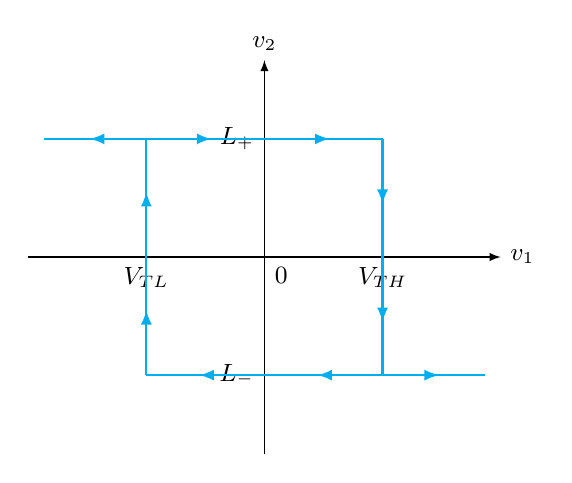
\begin{tikzpicture}[thick,>=latex, font=\small]

    % Custom style for placing arrows in the middle of a path segment
    \tikzset{
        midarrow/.style={
            decoration={markings, mark=at position 0.55 with {\arrow{latex}}},
            postaction={decorate}
        }
    }

    % ==========================================
    % Figure (i): Hysteresis Loop
    % ==========================================
    \begin{scope}[shift={(0,0)}]
        % Axes
        \draw[thin, ->] (-3,0) -- (3,0) node[right] {$v_1$};
        \draw[thin, ->] (0,-2.5) -- (0,2.5) node[above] {$v_2$};
        \node[below right] at (0,0) {$0$};
        
        % Axis Labels
        \node[below] at (-1.5,0) {$V_{TL}$};
        \node[below] at (1.5,0) {$V_{TH}$};
        \node[left] at (0, 1.5) {$L_+$};
        \node[left] at (0, -1.5) {$L_-$};
        
        % Characteristic Loop (Clockwise path)
        \draw[cyan, thick, midarrow] (-1.5, 1.5) -- (0, 1.5);
        \draw[cyan, thick, midarrow] (0, 1.5) -- (1.5, 1.5);
        \draw[cyan, thick, midarrow] (1.5, 1.5) -- (1.5, 0);
        \draw[cyan, thick, midarrow] (1.5, 0) -- (1.5, -1.5);
        \draw[cyan, thick, midarrow] (1.5, -1.5) -- (0, -1.5);
        \draw[cyan, thick, midarrow] (0, -1.5) -- (-1.5, -1.5);
        \draw[cyan, thick, midarrow] (-1.5, -1.5) -- (-1.5, 0);
        \draw[cyan, thick, midarrow] (-1.5, 0) -- (-1.5, 1.5);
        
        % Tails extending outwards
        \draw[cyan, thick, midarrow] (-1.5, 1.5) -- (-2.8, 1.5); % Extending left
        \draw[cyan, thick, midarrow] (1.5, -1.5) -- (2.8, -1.5); % Extending right
        
        % Caption
    \end{scope}

\end{tikzpicture}
\end{center}
\begin{center}
    
\begin{tikzpicture}[thick,>=latex, font=\small]

    % Custom style for placing arrows in the middle of a path segment
    \tikzset{
        midarrow/.style={
            decoration={markings, mark=at position 0.55 with {\arrow{latex}}},
            postaction={decorate}
        }
    }
    % ==========================================
    % Figure (ii): Square Waveform (Middle Plot)
    % ==========================================
    \begin{scope}[shift={(2.5,0)}]
        % Axes
        \draw[thin, ->] (-0.5,0) -- (4.5,0) node[right] {$t$};
        \draw[thin, ->] (0,-2.5) -- (0,2.5) node[above] {$v_2$};
        \node[below right] at (0,0) {$0$};
        
        % Y-axis Labels
        \node[left] at (0, 1.5) {$L_+$};
        \node[left] at (0, -1.5) {$L_-$};
        
        % Waveform path
        \draw[cyan, thick] (-0.5,-1.5) -- (0,-1.5) -- (0,1.5) -- (1.6,1.5) -- (1.6,-1.5) -- (3.6,-1.5) -- (3.6,1.5) -- (4.2,1.5);
        
        % Dimension arrows
        \draw[<->, thin] (0, 2.0) -- (1.6, 2.0) node[midway, fill=white, inner sep=1pt] {$T_1$};
        \draw[<->, thin] (1.6, 2.0) -- (3.6, 2.0) node[midway, fill=white, inner sep=1pt] {$T_2$};
        \draw[<->, thin] (0, -2.0) -- (3.6, -2.0) node[midway, fill=white, inner sep=1pt] {$T$};
        
        % Dashed reference lines
        \draw[dashed, thin] (1.6, 1.5) -- (1.6, 2.2);
        \draw[dashed, thin] (3.6, 1.5) -- (3.6, 2.2);
        \draw[dashed, thin] (0, 1.5) -- (0, 2.2);
        \draw[dashed, thin] (0, -1.5) -- (0, -2.2);
        \draw[dashed, thin] (3.6, -1.5) -- (3.6, -2.2);
    \end{scope}

    % ==========================================
    % Figure (ii): Triangular Waveform (Right Plot)
    % ==========================================
    \begin{scope}[shift={(12,0)}]
        % Axes
        \draw[thin, ->] (-0.5,0) -- (4.5,0) node[right] {$t$};
        \draw[thin, ->] (0,-2.5) -- (0,2.5) node[above] {$v_1$};
        \node[below right] at (0,0) {$0$};
        
        % Y-axis Labels
        \node[left] at (0, 1.5) {$V_{TH}$};
        \node[left] at (0, -1.5) {$V_{TL}$};
        
        % Waveform path (calculated slopes for precise geometric matching)
        \draw[cyan, thick] (-0.5, 0.75) -- (0, 1.5) -- (1.6, -1.5) -- (3.6, 1.5) -- (4.2, 0.375);
        
        % Dimension arrows
        \draw[<->, thin] (0, 2.0) -- (1.6, 2.0) node[midway, fill=white, inner sep=1pt] {$T_1$};
        \draw[<->, thin] (1.6, 2.0) -- (3.6, 2.0) node[midway, fill=white, inner sep=1pt] {$T_2$};
        
        % Dashed reference lines
        \draw[dashed, thin] (0, 1.5) -- (0, 2.2);
        \draw[dashed, thin] (1.6, -1.5) -- (1.6, 2.2);
        \draw[dashed, thin] (3.6, 1.5) -- (3.6, 2.2);
    \end{scope}
    

\end{tikzpicture}
\end{center}
\mk{18} \yr{EEE 263 | L-2/T-1 | Jan--2021}

\end{enumerate}


%% ══════════════════════════════════════════════════════════════════════
%%  PART VI
%% ══════════════════════════════════════════════════════════════════════
\secdivider{Part VI --- Digital Logic and Sequential Circuits}{CMOS logic design, flip-flops, counters, and digital circuit implementation}{cD}

%% ══════════════════════════════════════════════════════════════════════
%%  SECTION 9: DIGITAL LOGIC AND SEQUENTIAL CIRCUITS
%% ══════════════════════════════════════════════════════════════════════
\markboth{S9: Digital Logic \& Sequential Circuits}{S9: Digital Logic \& Sequential Circuits}
\label{sec:S9}
\titleformat{\section}{\large\bfseries\color{cD}}{}{0em}{}[\titlerule]
\section*{S9 \quad Digital Logic \& Sequential Circuits}
\addcontentsline{toc}{section}{S9: Digital Logic \& Sequential Circuits}

%%──────────────────────────────────────────────────────────────────────
\subtopic{cD}{CMOS Logic Design and Implementation}
\label{sub:s9-cmos}

\begin{enumerate}\item Discuss basic operational characteristics and parameters of CMOS and TTL logic families.
\mk{23} \yr{EEE 263 | L-2/T-1 | 2021--22}

\item Implement the function $f(A,B,C,D)=\sum m(0,4,8,9,10,11,12)$ using CMOS.
\mk{13} \yr{EEE 263 | L-2/T-1 | 2018--19}

\item Draw a CMOS complex gate for the logic function $f(a,b,c,d)=\sum m(0,1,2,4,6,8,10,12,14)$. Use as few transistors as possible.
\mk{15} \yr{EEE 263 | L-2/T-1 | 2017--18}

\item Derive complex gates for the following logic functions using as few transistors as possible:
\begin{enumerate}
  \item $f(X_1,X_2,X_3,X_4)=\sum m(0,4,6,8,9,15)+D(3,7,11,13)$
  \item $\bar{f}=(A+B)(C+D)(\bar{A}+B+D)$
\end{enumerate}
\mk{21} \yr{EEE 263 | L-2/T-1 | 2016--17}

\item Implement the function $f(A,B,C,D)=\sum m(1,2,4,7,14,15)$ using (i) CMOS circuit and (ii) pseudo NMOS circuit. Which circuit would you prefer between your two designed circuits and why?
\mk{25} \yr{EEE 263 | L-2/T-1 | Jan--2021}

\end{enumerate}

%%──────────────────────────────────────────────────────────────────────
\subtopic{cD}{CMOS Transistor Sizing}
\label{sub:s9-sizing}

\begin{enumerate}\item Calculate transistor $W/L$ ratios for the logic circuit shown. Assume that for the basic inverter $n=1.5$ and $P=5$ and the channel length is 0.25\,$\mu$m.
\begin{center}
    \begin{circuitikz}[thick,american, scale=1.3]

    % ==========================================
    % Power Supply (VDD)
    % ==========================================
    \draw[thick] (0, 4.6) -- (0, 5.0);
    \draw[->, thick] (0, 4.8) -- (0, 5.3) node[above] {$V_{DD}$};

    % ==========================================
    % Pull-Up Network (PMOS)
    % ==========================================
    % Transistor QPA
    \node[pmos] (QPA) at (0, 4.0) {};
    \node[right=0.3cm] at (QPA) {$Q_{PA}$};
    \draw (QPA.G) -- ++(-0.4, 0) node[ocirc] {} node[left] {A};

    % Split below QPA
    \coordinate (split_top) at (0, 3.2);
    \draw (QPA.D) -- (split_top);
    
    % Parallel branches for QPB and QPC
    \draw (split_top) -- (-1.2, 3.2);
    \draw (split_top) -- (1.2, 3.2);

    % Transistor QPB
    \node[pmos] (QPB) at (-1.2, 2.2) {};
    \node[right=0.3cm] at (QPB) {$Q_{PB}$};
    \draw (-1.2, 3.2) -- (QPB.S);
    \draw (QPB.G) -- ++(-0.4, 0) node[ocirc] {} node[left] {B};

    % Transistor QPC
    \node[pmos] (QPC) at (1.2, 2.2) {};
    \node[right=0.3cm] at (QPC) {$Q_{PC}$};
    \draw (1.2, 3.2) -- (QPC.S);
    \draw (QPC.G) -- ++(-0.4, 0) node[ocirc] {} node[left] {C};

    % Merge below QPB and QPC
    \coordinate (merge_p) at (0, 1.2);
    \draw (QPB.D) -- (-1.2, 1.2) -- (1.2, 1.2) -- (QPC.D);

    % ==========================================
    % Output Node Y
    % ==========================================
    \coordinate (out_node) at (0, 0.7);
    \draw (merge_p) -- (out_node);
    \node[circ] at (out_node) {};
    \draw (out_node) -- ++(2.0, 0) node[ocirc] {} node[right] {Y};

    % ==========================================
    % Pull-Down Network (NMOS)
    % ==========================================
    \coordinate (split_n) at (0, 0.2);
    \draw (out_node) -- (split_n);
    
    % Parallel branches for NMOS
    \draw (split_n) -- (-1.2, 0.2);
    \draw (split_n) -- (1.2, 0.2);

    % Transistor QNA (Left Branch)
    \node[nmos] (QNA) at (-1.2, -0.8) {};
    \node[right=0.3cm] at (QNA) {$Q_{NA}$};
    \draw (-1.2, 0.2) -- (QNA.D);
    \draw (QNA.G) -- ++(-0.4, 0) node[ocirc] {} node[left] {A};

    % Transistors QNB and QNC (Right Branch - Series)
    \node[nmos] (QNB) at (1.2, -0.4) {};
    \node[right=0.3cm] at (QNB) {$Q_{NB}$};
    \draw (1.2, 0.2) -- (QNB.D);
    \draw (QNB.G) -- ++(-0.4, 0) node[ocirc] {} node[left] {B};

    \node[nmos] (QNC) at (1.2, -1.6) {};
    \node[right=0.3cm] at (QNC) {$Q_{NC}$};
    \draw (QNB.S) -- (QNC.D);
    \draw (QNC.G) -- ++(-0.4, 0) node[ocirc] {} node[left] {C};

    % ==========================================
    % Ground Connection
    % ==========================================
    \coordinate (ground_rail) at (0, -2.4);
    \draw (QNA.S) -- (-1.2, -2.4) -- (1.2, -2.4) -- (QNC.S);
    \node[circ] at (ground_rail) {};
    \draw (ground_rail) node[ground] {};

    % ==========================================
    % Caption
    % ==========================================

\end{circuitikz}
\end{center}
\mk{16} \yr{EEE 263 | L-2/T-1 | 2018--19}

\item Design transistor $W/L$ ratios for the logic $Y=\overline{(AB+D)C}$ implemented using CMOS circuit. Assume that for the basic inverter $(W/L)_n=n=2$ and $(W/L)_p=p=7$ and the channel length is 0.15\,$\mu$m.
\mk{21} \yr{EEE 263 | L-2/T-1 | Jan--2021}

\end{enumerate}

%%──────────────────────────────────────────────────────────────────────
\subtopic{cD}{Inverter Propagation Delay}
\label{sub:s9-delay}

\begin{enumerate}\item For the inverter shown with a capacitor $C$ connected between the output node and ground: if at $t=0$ the input goes low to high, find the equation of time for $v_0$ to reach $\frac{1}{2}(V_{OL}+V_{OH})$. Also calculate the high-to-low propagation time for $R=25\,\text{k}\Omega$ and $C=20\,\text{pF}$.
\begin{center}
    \begin{circuitikz}[thick,american, scale=1.3]
                \ctikzset{tripoles/mos style/arrows}

    % ==========================================
    % NMOS Transistor & Input
    % ==========================================
    \node[nmos] (M1) at (0,0) {};
    \draw (M1.G) -- ++(-0.6, 0) node[ocirc] {} node[left] {$v_I$};
    
    % ==========================================
    % Source Connection (Ground)
    % ==========================================
    % Define a coordinate for the source ground to align the capacitor later
    \draw (M1.S) -- ++(0, -0.5) coordinate (gnd_s) node[ground] {};
    
    % ==========================================
    % Drain Connection (Pull-up Resistor & VDD)
    % ==========================================
    % l_=$R$ places the label on the right side of the upward drawing path
    \draw (M1.D) node[circ] {} to[R, l_=$R$] ++(0, 2.0) node[ocirc] {} node[right] {$V_{DD}=5\text{V}$};
    
    % ==========================================
    % Output Branch & Load Capacitor
    % ==========================================
    % Draw horizontal line from drain to the output junction
    \draw (M1.D) -- ++(1.5, 0) coordinate (out_junc);
    
    % Continue to the output terminal
    \draw (out_junc) node[circ] {} -- ++(0.6, 0) node[ocirc] {} node[right] {$v_o$};
    
    % Draw the capacitor down to ground, perfectly aligned horizontally with the source ground
    \draw (out_junc) to[C, l_=$C$] (out_junc |- gnd_s) node[ground] {};

\end{circuitikz}
\end{center}
\mk{10.67} \yr{EEE 263 | L-2/T-1 | 2018--19}

\end{enumerate}

%%──────────────────────────────────────────────────────────────────────
\subtopic{cD}{Transmission Gate Implementation}
\label{sub:s9-tg}

\begin{enumerate}\item Implement the following function $Y$ using CMOS transmission gate configuration:
\[
Y = AB + \bar{A}C
\]
\mk{7} \yr{EEE 263 | L-2/T-1 | 2018--19}

\end{enumerate}

%%──────────────────────────────────────────────────────────────────────
\subtopic{cD}{CMOS Flip-Flop Implementation}
\label{sub:s9-ff-cmos}

\begin{enumerate}\item Show a CMOS implementation of edge-triggered D flip-flops with asynchronous reset.
\mk{25} \yr{EEE 263 | L-2/T-1 | 2016--17}

\end{enumerate}

%%──────────────────────────────────────────────────────────────────────
\subtopic{cD}{Flip-Flop Construction}
\label{sub:s9-ff-construction}

\begin{enumerate}\item Show how D flip-flop and T flip-flop can be constructed from J-K flip-flops.
\mk{15} \yr{EEE 263 | L-2/T-1 | 2016--17}

\end{enumerate}

%%──────────────────────────────────────────────────────────────────────
\subtopic{cD}{Counter Design}
\label{sub:s9-counter}

\begin{enumerate}\item Design a MOD-3 counter using JK flip-flops and verify the design showing the truth table.
\mk{15} \yr{EEE 263 | L-2/T-1 | 2021--22}

\item Design a modulo-12 up counter with synchronous reset.
\mk{15} \yr{EEE 263 | L-2/T-1 | 2017--18}

\item Design a 4-bit up/down counter using T flip-flops. It should include a control pin $\overline{UP}/DOWN$. When $\overline{UP}/DOWN=0$ the circuit behaves as an up counter; when $\overline{UP}/DOWN=1$ it behaves as a down counter. The circuit should also have a synchronous active-low $\overline{RESET}$ pin.
\mk{20} \yr{EEE 263 | L-2/T-1 | 2016--17}

\end{enumerate}

%%──────────────────────────────────────────────────────────────────────
\subtopic{cD}{Combinational Logic Design}
\label{sub:s9-combo}

\begin{enumerate}\item Draw a PLA programmed to implement the following functions:
\begin{align*}
Y_1 &= A\bar{B}C + \bar{A}C + B \\
Y_2 &= \bar{B}AC + AB\bar{C} + \bar{B} \\
Y_3 &= \bar{A}C + B\bar{C}A
\end{align*}
\mk{15} \yr{EEE 263 | L-2/T-1 | 2017--18}

\item Implement the function $f(x_1,x_2,x_3)=\sum m(2,3,4,6,7)$ using two-input LUTs (Look Up Tables). You can use as many LUTs as needed.
\mk{16} \yr{EEE 263 | L-2/T-1 | 2017--18}

\item Triangular numbers are sequences formed by continuous summation of natural numbers (1, 3, 6, 10, \ldots). Design the simplest possible logic circuit that outputs 1 whenever it detects a 4-bit triangular number.

\begin{center}
        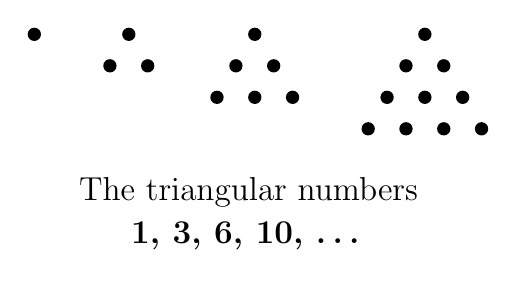
\begin{tikzpicture}[scale=0.8]
        
        % 1st triangular number (1)
        \fill (0,0) circle (3pt);
        
        % 2nd triangular number (3)
        \begin{scope}[xshift=1.5cm]
            \fill (0,0) circle (3pt);
            \fill (-0.3,-0.5) circle (3pt);
            \fill (0.3,-0.5) circle (3pt);
        \end{scope}
        
        % 3rd triangular number (6)
        \begin{scope}[xshift=3.5cm]
            \fill (0,0) circle (3pt);
            \fill (-0.3,-0.5) circle (3pt);
            \fill (0.3,-0.5) circle (3pt);
            \fill (-0.6,-1.0) circle (3pt);
            \fill (0,-1.0) circle (3pt);
            \fill (0.6,-1.0) circle (3pt);
        \end{scope}
        
        % 4th triangular number (10)
        \begin{scope}[xshift=6.2cm]
            \fill (0,0) circle (3pt);
            \fill (-0.3,-0.5) circle (3pt);
            \fill (0.3,-0.5) circle (3pt);
            \fill (-0.6,-1.0) circle (3pt);
            \fill (0,-1.0) circle (3pt);
            \fill (0.6,-1.0) circle (3pt);
            \fill (-0.9,-1.5) circle (3pt);
            \fill (-0.3,-1.5) circle (3pt);
            \fill (0.3,-1.5) circle (3pt);
            \fill (0.9,-1.5) circle (3pt);
        \end{scope}
        
        % Text elements
        \node at (3.4, -2.5) {\large The triangular numbers};
        \node at (3.4, -3.2) {\large \textbf{1, 3, 6, 10, \dots}};
        
    \end{tikzpicture}
\end{center}

\mk{11} \yr{EEE 263 | L-2/T-1 | 2016--17}

\end{enumerate}

%%──────────────────────────────────────────────────────────────────────
\subtopic{cD}{Priority Encoder}
\label{sub:s9-encoder}

\begin{enumerate}\item Design a four-line to two-line priority encoder circuit with active high inputs and outputs, with priority assigned to the higher-order data input line ($I_4 > I_3 > I_1$). Use NOR gates only for the circuit implementation.
\mk{16} \yr{EEE 263 | L-2/T-1 | 2017--18}

\end{enumerate}

%%──────────────────────────────────────────────────────────────────────
\subtopic{cD}{Shift Register Design}
\label{sub:s9-shift}

\begin{enumerate}\item Design a 4-bit shift register using D flip-flops and a four-to-one multiplexer with mode selection inputs $S_1$ and $S_0$. The register operates according to the following function table:
\begin{center}
\begin{tabular}{ccl}
\toprule
$S_1$ & $S_0$ & \textbf{Register Operation} \\
\midrule
0 & 0 & No change \\
0 & 1 & Complement the four outputs \\
1 & 0 & Clear register to 0 (synchronous with clock) \\
1 & 1 & Shift Right \\
\bottomrule
\end{tabular}
\end{center}
\mk{15} \yr{EEE 263 | L-2/T-1 | 2017--18}

\end{enumerate}

%% ══════════════════════════════════════════════════════════════════════
%%  PART VII
%% ══════════════════════════════════════════════════════════════════════
\secdivider{Part VII --- Data Converters, PLL \& Memory}{DAC, ADC, Phase-Locked Loop, DRAM, Flash Memory}{cH}

%% ══════════════════════════════════════════════════════════════════════
%%  SECTION 10: DATA CONVERTERS, PLL & MEMORY
%% ══════════════════════════════════════════════════════════════════════
\markboth{S10: Data Converters, PLL \& Memory}{S10: Data Converters, PLL \& Memory}
\label{sec:S10}
\titleformat{\section}{\large\bfseries\color{cH}}{}{0em}{}[\titlerule]
\section*{S10 \quad Data Converters, PLL \& Memory}
\addcontentsline{toc}{section}{S10: Data Converters, PLL \& Memory}

%%──────────────────────────────────────────────────────────────────────
\subtopic{cH}{Digital-to-Analog Converter (DAC)}
\label{sub:s10-dac}

\begin{enumerate}\item What are DAC circuits? How does an R-2R ladder DAC circuit operate? Explain using a circuit diagram and mathematical analysis.
\mk{17} \yr{EEE 263 | L-2/T-1 | 2021--22}

\end{enumerate}

%%──────────────────────────────────────────────────────────────────────
\subtopic{cH}{Analog-to-Digital Converter (ADC)}
\label{sub:s10-adc}

\begin{enumerate}\item A 6-bit A/D converter has reference voltage $V_{REF}=8\,\text{V}$ and reference count $n_{REF}=2^6$. Values of some consecutive analog sampled voltages $|V_A|$ are: 0\,V, 3\,V, 5.5\,V, 7.125\,V. If these voltages are given as inputs to the converter, find the corresponding digital outputs.
\mk{12} \yr{EEE 263 | L-2/T-1 | 2021--22}

\end{enumerate}

%%──────────────────────────────────────────────────────────────────────
\subtopic{cH}{Phase-Locked Loop (PLL)}
\label{sub:s10-pll}

\begin{enumerate}\item Draw a simplified block diagram of a PLL and briefly explain its operation.
\mk{17} \yr{EEE 263 | L-2/T-1 | 2021--22}

\end{enumerate}

%%──────────────────────────────────────────────────────────────────────
\subtopic{cH}{Memory: DRAM and Flash}
\label{sub:s10-memory}

\begin{enumerate}\item Explain the read and write operation in a DRAM cell.
\mk{16} \yr{EEE 263 | L-2/T-1 | 2021--22}

\item Explain briefly the programming and erase operation in a Flash Memory.
\mk{15} \yr{EEE 263 | L-2/T-1 | 2021--22}

\end{enumerate}

\end{document}